% Customizable fields and text areas start with % >> below.
% Lines starting with the comment character (%) are normally removed before release outside the collaboration, but not those comments ending lines

% svn info. These are modified by svn at checkout time.
% The last version of these macros found before the maketitle will be the one on the front page,
% so only the main file is tracked.
% Do not edit by hand!
\RCS$Revision: 274812 $
\RCS$HeadURL: svn+ssh://tahuang@svn.cern.ch/reps/tdr2/notes/DN-13-022/tags/1.0/DN-13-022.tex $
\RCS$Id: DN-13-022.tex 274812 2015-01-23 23:10:51Z pakhotin $
%%%%%%%%%%%%% local definitions %%%%%%%%%%%%%%%%%%%%%
% This allows for switching between one column and two column (cms@external) layouts
% The widths should  be modified for your particular figures. You'll need additional copies if you have more than one standard figure size.
\newlength\cmsFigWidth
\ifthenelse{\boolean{cms@external}}{\setlength\cmsFigWidth{0.85\columnwidth}}{\setlength\cmsFigWidth{0.4\textwidth}}
\ifthenelse{\boolean{cms@external}}{\providecommand{\cmsLeft}{top}}{\providecommand{\cmsLeft}{left}}
\ifthenelse{\boolean{cms@external}}{\providecommand{\cmsRight}{bottom}}{\providecommand{\cmsRight}{right}}
%%%%%%%%%%%%%%%  Title page %%%%%%%%%%%%%%%%%%%%%%%%
\cmsNoteHeader{DN-13-022} % This is over-written in the CMS environment: useful as preprint no. for export versions
% >> Title: please make sure that the non-TeX equivalent is in PDFTitle below
\title{Improvements to ME1/1 Trigger Motherboard Algorithm for Operation under High Pile-Up Running Conditions}

% >> Authors
%Author is always "The CMS Collaboration" for PAS and papers, so author, etc, below will be ignored in those cases
%For multiple affiliations, create an address entry for the combination
%To mark authors as primary, use the \author* form
\address[ghent]{Ghent University}
\address[tamu]{Texas A\&M University}
\address[ucla]{University of California, Los Angeles}
\address[osaka]{University of Seoul}
\address[ufl]{Univerosity of Florida}
\author[ghent]{Sven Dildick}
\author[tamu]{Jose Roberto Dimas Valle}
\author[ucla]{Jay Hauser}
\author[tamu]{Tao Huang}
\author[tamu]{Vadim Khotilovich}
\author[tamu]{Vyacheslav Krutelyov}
\author[osaka]{Jason Lee}
\author[ufl]{Alexander Madorsky}
\author[tamu]{Yuriy Pakhotin}
\author[ucla]{Andrew Peck}
\author[tamu]{Alexei Safonov}
\author[tamu]{Aysen Tatarinov}
\author[ucla]{Vyacheslav Valuev}

% >> Date
% The date is in yyyy/mm/dd format. Today has been
% redefined to match, but if the date needs to be fixed, please write it in this fashion.
% For papers and PAS, \today is taken as the date the head file (this one) was last modified according to svn: see the RCS Id string above.
% For the final version it is best to "touch" the head file to make sure it has the latest date.
\date{\today}

% >> Abstract
% Abstract processing:
% 1. **DO NOT use \include or \input** to include the abstract: our abstract extractor will not search through other files than this one.
% 2. **DO NOT use %**                  to comment out sections of the abstract: the extractor will still grab those lines (and they won't be comments any longer!).
% 3. For PASs: **DO NOT use tex macros**         in the abstract: CDS MathJax processor used on the abstract doesn't understand them _and_ will only look within $$. The abstracts for papers are hand formatted so macros are okay.
\abstract{
Improvements to ME1/1 trigger motherboard algorithm for operation under high pile-up conditions are described as well as details of their configuration in software. Individual effects of these improvements on ME1/1 trigger efficiency are quantified and ranked in terms of their importance in simulation studies.
}

% >> PDF Metadata
% Do not comment out the following hypersetup lines (metadata). They will disappear in NODRAFT mode and are needed by CDS.
% Also: make sure that the values of the metadata items are sensible and are in plain text:
% (1) no TeX! -- for \sqrt{s} use sqrt(s) -- this will show with extra quote marks in the draft version but is okay).
% (2) no %.
% (3) No curly braces {}.
\hypersetup{%
pdfauthor={Aysen Tatarinov},%
pdftitle={Improvements to ME1/1 Trigger Motherboard Algorithm for Operation under High Pile-Up Running Conditions},%
pdfsubject={CMS},%
pdfkeywords={LHC, CMS, Muons, CSC, Trigger}}

\maketitle %maketitle comes after all the front information has been supplied
% >> Text
%%%%%%%%%%%%%%%%%%%%%%%%%%%%%%%%  Begin text %%%%%%%%%%%%%%%%%%%%%%%%%%%%%
%% **DO NOT REMOVE THE BIBLIOGRAPHY** which is located before the appendix.
%% You can take the text between here and the bibiliography as an example which you should replace with the actual text of your document.
%% If you include other TeX files, be sure to use "\input{filename}" rather than "\input filename".
%% The latter works for you, but our parser looks for the braces and will break when uploading the document.

\tableofcontents

\newpage
\tracinginput{sections/introduction.tex}
%\section{Introduction}

The muon trigger is a tracking trigger that measures the momentum of muons using the magnetic field in the steel yoke of the CMS detector~\cite{Chatrchyan:2008zzk}; thus its resolution degrades with increasing momentum. This can be improved by maximizing the number of chamber hits along a muon trajectory and by improving the precision and number of position and angular measurements participating in the track fit applied in the trigger logic. The focus of the muon trigger upgrade is to improve its rate reduction capability without significantly affecting the efficiency.

The philosophy applied to the design of the present muon trigger was to preserve the complementarity and redundancy of the three separate muon detection systems until they are combined at the input to the Global Trigger. In contrast, the upgrade to the muon trigger will utilize the redundancy of the three muon detection systems earlier in the trigger processing chain so as to obtain a more performant trigger with higher efficiency and better rate reduction. Recognizing that every additional hit along a muon trajectory further improves the fake rejection and muon momentum measurement, the upgrade seeks to combine muon hits at the input stage to the Muon Track-Finder layer rather than at its output, given the successful operation of all three muon detection systems in the LHC Run 1. This new Muon Track-Finder will ultimately replace the separate track-finders for the Drift-Tube (DT) and Cathode Strip Chamber (CSC) muon triggers as well as the Resistive Plate Chamber (RPC) pattern comparator trigger. However, in addition to combining data from multiple muon systems in the same processors, more robust and sophisticated algorithms will be applied that are tolerant of the increased pile-up and make better use of the data from each muon system in the track-finding and $p_T$ measurement. Present and upgraded muon trigger algorithms in CSC are described in Section~\ref{sec:present_algo} and Section~\ref{sec:SLHC_algo}, correspondingly. Individual improvements of the upgraded algorithm are studied in Section~\ref{sec:SLHC_algo_results}.

The muon trigger upgrade is not expected to be completed before the LHC resumes operation after Long Shutdown I in 2015. Thus it is imperative to be able to commission the new muon trigger in parallel with the operation of the current trigger. For that reason, the trigger primitives from the CSC and RPC systems will be fully split into two paths, and those from the DT system will be split from a slice of the system. Data concentration into high bandwidth links for all three systems should be available for at least a slice of the detector as input to the new trigger in 2015. The goal is to have the entire muon trigger upgrade commissioned during the 2015-16 Year-End Technical Stop, so that the new trigger will be available in 2016. Recognizing the physics importance of the first year of LHC running at a higher center-of-mass energy ($\sqrt{s} = 13$~TeV) in 2015, a provision is foreseen to apply isolation criteria to the CSC muons in the forward region of the detector using the energy deposits in the calorimeter. This will allow to maintain relatively low $p_T$ thresholds reducing the rate of muons from heavy flavor jets despite the higher collision energy and higher luminosity.

As a part of future upgrade for Phase II of LHC running, the CMS will be equiped with Gas Electron Multiplier (GEM) detectors in the high pseudorapidity region ($1.5 < |\eta| < 2.2$). Pairs of triple-GEM chambers will be installed in the currently vacant position in front of the ME1/1 chambers and are dubbed GE1/1. The addition of such chambers allows to measure the bending angle of a track between GE1/1 and ME1/1. Usage of the bending angle at L1 can help to keep the rates down while keeping the efficiency high. In section \ref{sec:slhc_algorithm_with_gems} we investigate several implementation possibilities of the combined GEM-CSC trigger algorithm for the high luminosity run of SLHC.
\clearpage

\newpage
\tracinginput{sections/muon_trigger.tex}
%\section{Present Muon Trigger}

\subsection{Global Trigger Data-Flow}

Each of the three muon detector systems in CMS participates in the Level-1 (L1) muon trigger for coverage and redundancy. For the DT and CSC systems ($|\eta|$ $<$ 1.2 and $|\eta|$ $>$ 0.9, respectively), the front-end trigger primitive generator (TPG) electronics identify track segments from the hit information registered in multiple gas planes of a single measurement station. These segments are collected and then transmitted via optical fibres to regional Track-Finders in the electronics service cavern, which then apply pattern recognition algorithms in order to identify muon candidates and measure their momenta from the magnetic bending in the return yoke between several measurement stations. Information is shared between the DT Track-Finder (DTTF) and CSC Track-Finder (CSCTF) for efficient coverage in the region of overlap between the two systems at $|\eta|$ $\approx 1$. The hits from the RPC system ($|\eta|<1.6$) are directly sent from the front-end electronics to Pattern Comparator (PAC) logic boards that identify muon candidates.

The three regional track-finders sort the identified muon candidates and transmit to the Global Muon Trigger (GMT) up to 4 (CSCTF, DTTF) or 8 (RPC) candidates every bunch crossing. Each candidate has been assigned a $p_T$ and quality code as well as $\eta$ and $\phi$ positions in the muon system (with a granularity of $\approx 0.05$). The GMT then merges muon candidates found by more than one system to eliminate fake multi-muon triggers (with several options on how to select $p_T$ between the candidates), and can suppress muon candidates in some regions of the detector if their quality is low and they are unconfirmed by another muon detector system. The data flow of the present L1 muon trigger is shown in Fig.~\ref{fig:l1_muon_trig}.

\begin{figure}[b]
	\begin{center}
		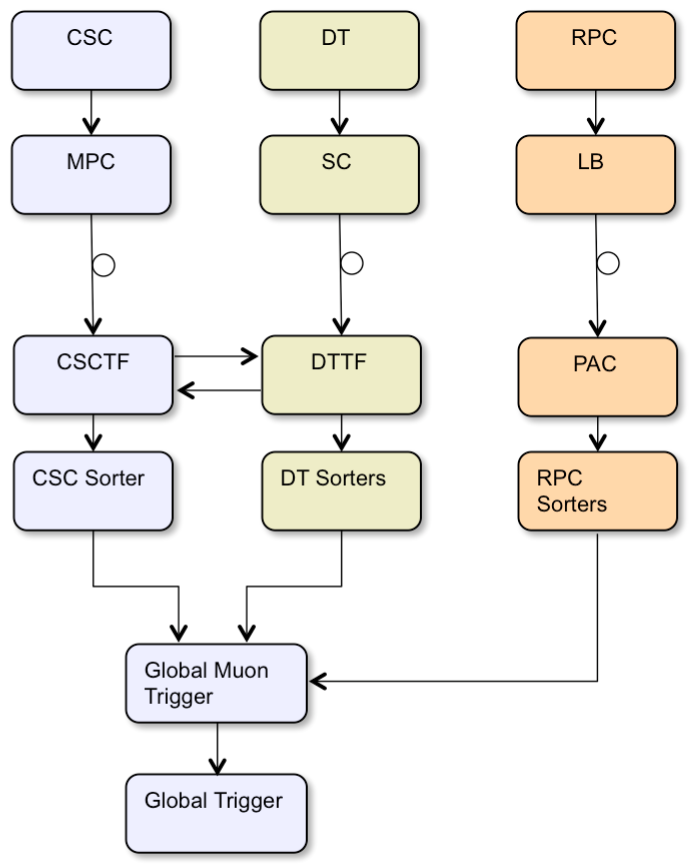
\includegraphics[width=0.48\linewidth]{figures/dataflow_current_L1_trigger.png}
	\end{center}
	\caption{Data-flow of the present L1 muon trigger. \label{fig:l1_muon_trig} }
\end{figure}

\subsection{Muon Trigger in Endcaps}

Each CSC can provide up to two local charged track (LCT) segments to the trigger logic per bunch crossing (BX, where 1 BX = 25 ns). These are formed in the trigger motherboard (TMB) combining cathode (CLCT) and anode (ALCT) segments. Present and improved logics of the algorithm which constructs LCTs are described in Section~\ref{sec:present_algo} and Section~\ref{sec:SLHC_algo}, respectively. The CLCT data contains information on the azimuthal position of the segment ($\phi$), the bend angle, and the pattern of cathode half-strips with hits in a chamber. The ALCT data contains information on the radial position from the beamline of the segment (equivalent to $\eta$), and the pattern of anode wires with hits in a chamber. The timing information from anodes is used to define the time of the combined LCT. There is one TMB per CSC, located in a crate on the periphery of the detector. The TMB sends up to two LCTs over a custom backplane to the muon port card (MPC), which is located in the same peripheral crate. One MPC can receive data from up to 9 TMBs, or equivalently, can receive up to 18 LCTs. The LCTs in a MPC are sorted by rank (see definition in MPC documentation). The best three LCTs are sent over optical fibers to the CSCTF. There are a total of sixty peripheral crates for the CSC system, each with one MPC.

The CSCTF system is partitioned into sectors, each of which corresponds to a $60^{o}$ azimuthal region of an endcap. Twelve ``sector processors'' are required for the entire endcap muon system, six per endcap. Each sector processor is a 9U VME card that is housed in a single crate. Three 1.6 Gb/s optical links from each of five MPCs are received by each sector processor, for a total of 180 optical links for the entire system. The CSCTF sectors are independent, since there is no sharing of data across boundaries of neighboring sectors, leading to slight inefficiencies.

There are several Field Programmable Gate Arrays (FPGAs) on each ``sector processor'', but the main FPGA for the track-finding algorithms is from the Xilinx Virtex-5 family. The conversion of strip and wire positions of each track segment to ($\eta, \phi$) coordinates is accomplished via a set of cascaded SRAM look-up tables (LUTs), each $512K\times16$ bits. These coordinates are then used for track-finding and momentum assignment.

The CSCTF track-finding logic consists of pairwise comparisons of track segments in different detector stations. These test for compatibility in $\phi$ and $\eta$ with a muon emanating from the collision vertex within certain tolerance windows. The comparisons are then analyzed and built into tracks consisting of possibly more than two segments from different stations. Possible duplicate (“ghost”) tracks are canceled. The track-finding logic has the ability to accept segments in different assigned bunch crossings by analyzing across a sliding time window of programmable length (nominally 2 BX) every bunch crossing. Duplicate tracks found on consecutive bunch crossings are canceled. The bunch crossing of a track is given by the second arriving track segment.

The $p_T$ of a muon candidate is calculated by using a large LUT implemented in SRAM. Information such as the track type, track $\eta$, the segment $\phi$ differences between a maximum of 3 stations, and the segment bend angle in the first measurement station are used to calculate the LUT address.

In addition to identifying muons from proton collisions, the CSCTF processors also simultaneously identifies any beam halo muons for monitoring and veto purposes by looking for trajectories approximately parallel to the beam line.

Each CSCTF sends up to three muon candidates per bunch crossing over a custom backplane to a muon sorter (MS). The MS then sorts the candidates by momentum and quality and selects the best 4 for the GMT. The CSCTF data are also sent to a DAQ card with SLINK interface which puts the trigger data into the event record.

\clearpage

\newpage
\tracinginput{sections/csc.tex}
%\section{CSC Upgrade During LS1}
\label{sec:csc}

During LS1, the outermost ring of the fourth disk of chambers of each endcap (ME4/2) will be installed. This will result in four measurement stations for muons in the region 1.25 $<$ $|\eta|$ $<$ 1.8 providing the additional redundancy needed in a high rate environment. For the L1 trigger, this coverage will improve the efficiency of the CSCTF, and improve the rate reduction since it will be more likely to have 3 or more hits used in the $p_T$ assignment logic. No additional hardware or reconfiguration of the present Level-1 trigger is required. The MPCs for the fourth
disk already are in place and the present CSCTF already has logic in place for these chambers. This redundancy will extend to the more powerful algorithms envisioned for the muon trigger upgrade as well.

The electronics for the CSC system are also under major revision. The innermost chambers of the first endcap disks (ME1/1) provide a key sagitta measurement for the L1 muon trigger in the region $1.6 < |\eta| < 2.4$. These chambers will receive new digital cathode front-end boards (DCFEB) as well as new trigger and data acquisition electronics that will significantly enhance their performance in the trigger and in offline reconstruction. The strips of the ME1/1 chambers are split into two regions at $|\eta|$ = 2.1. The bottom region $|\eta| > 2.1$ currently has strips triple-ganged in the electronics for both the trigger and readout, making it ambiguous as to which third of the chamber generated a particular hit (the ganging has every 16th strip ganged to each other, where there are 48 strips in total across a chamber layer). The ambiguity can be mitigated using measurements from the outer stations. The $p_T$ resolution using only the outer stations is quite coarse, leading to a significantly increased single muon trigger rate in the region $2.1<|\eta|<2.4$. This forward region currently generates a single muon trigger rate comparable to that of the entire
region $|\eta| < 2.1$. With the new digital front-end boards and Trigger Motherboards (TMBs), this triple-ganging will be removed, leading to much improved triggering for $2.1<|\eta|<2.4$. This should allow CMS to maintain full muon trigger coverage up to $|\eta| = 2.4$ after LS1. The recovered older electronics will be used to instrument the new ME4/2 chambers.

\begin{figure}[htb]
        \begin{center}
                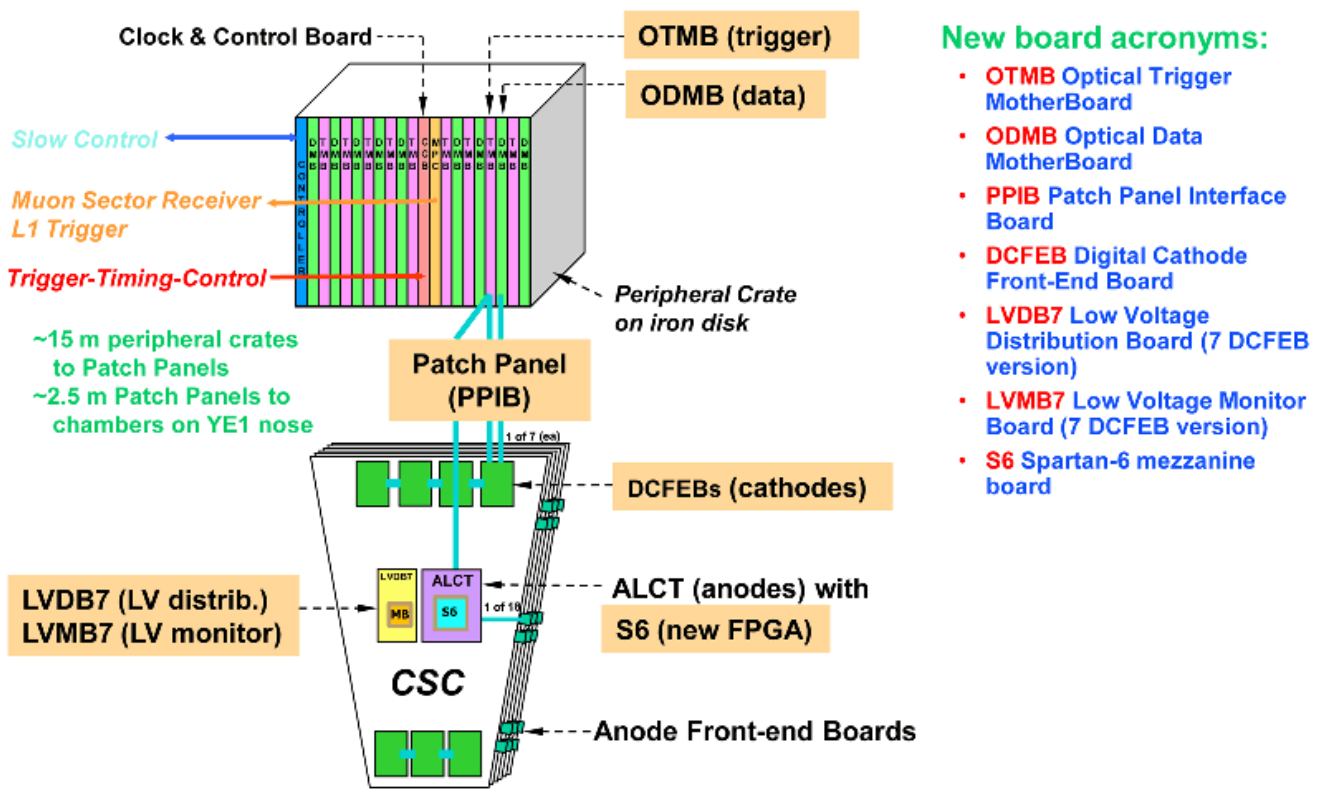
\includegraphics[width=0.90\linewidth]{figures/ME11_upgrade_overview.png}
                \caption{Schematic overview of the ME1/1 chambers upgrade.}
                \label{fig:me11_upgrade_overview}
        \end{center}
\end{figure}

\begin{figure}[htb]
        \begin{center}
                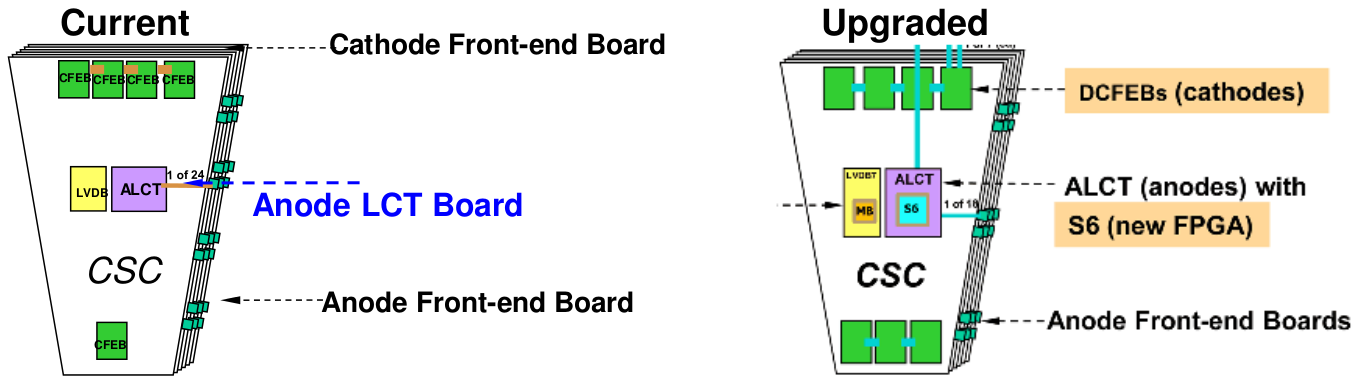
\includegraphics[width=0.90\linewidth]{figures/ME11_upgrade_electronics.png}
                \caption{Schematic overview of the ME1/1 electronics upgrade.}
                \label{fig:me11_upgrade_electronics}
        \end{center}
\end{figure}
\clearpage

\newpage
\tracinginput{sections/algorithm_2007.tex}
%\section{Present CSC Trigger Algorithm}
\label{sec:present_algo}

\subsection{ALCT Processing}

Anode wires in CSC are hardwired together at the readout end in groups of 10-15 wires in order to reduce channel count. The anode wire group (WG) signals are fed into the anode front-end boards (AFEBs), each of which contains a single 16-channel amplifier/constant-fraction discriminator chip. The output signals from the AFEBs are sent into the ALCT on-chamber board, which handles triggering and readout of the CSC anode information. Due to the various sizes of CSCs, there are 3 types of ALCT boards, handling 288, 384, and 672 anode wire group channels.

On the ALCT boards, the signals from each AFEB are first delayed by a programmable amount of time in order to perform an average time alignment of the anode signals across the chamber as well as chamber-to-chamber at a sub-bunch crossing level to about 2.2 ns precision. After the AFEB signals are received and time-aligned, then they are latched with bunch crossing frequency and fed to a FPGA (Xilinx Virtex family) mounted on a mezzanine card above the ALCT main board for pattern-finding and readout functions.

The algorithm used in the ALCT FPGA for determining muon segment position and bunch crossing is illustrated below. Since the drift time can be longer than 50 ns, the hits are first stretched by 'one-shots' to 6 BX (150 ns) length. Then, a multi-layer coincidence technique in the ALCT pattern circuitry is used to identify the bunch crossing. For each spatial pattern of anode hits, a low coincidence level, typically 2 or more layers, is used to establish timing, whereas a higher coincidence level, typically 4 layers, is used to establish the existence of a muon track. The general idea of a spatial pattern of CSC wire group hits is illustrated below in Fig.\ref{fig:anode_wire_group_hits}.

\begin{figure}[tbh]
        \begin{center}
                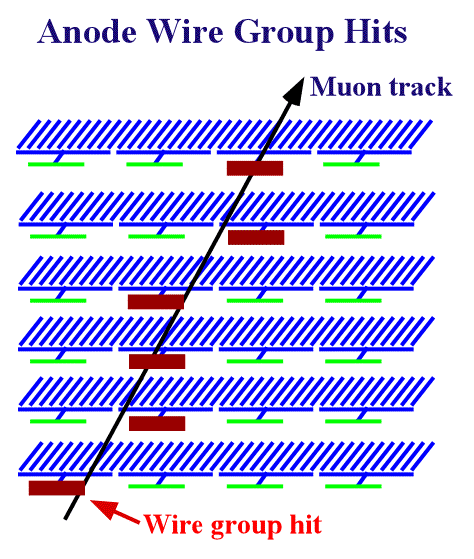
\includegraphics[width=0.48\linewidth]{figures/anode_wire_group_hits.png}
                \caption{CSC wire group patterns}
                \label{fig:anode_wire_group_hits}
        \end{center}
\end{figure}

while the general idea of the time stretching of hits, and pretrigger followed by a pattern trigger is shown in Fig.\ref{fig:anode_stretched_hits} (using an example in which one hit is actually missing due to some type of inefficiency).

\begin{figure}[tbh]
        \begin{center}
                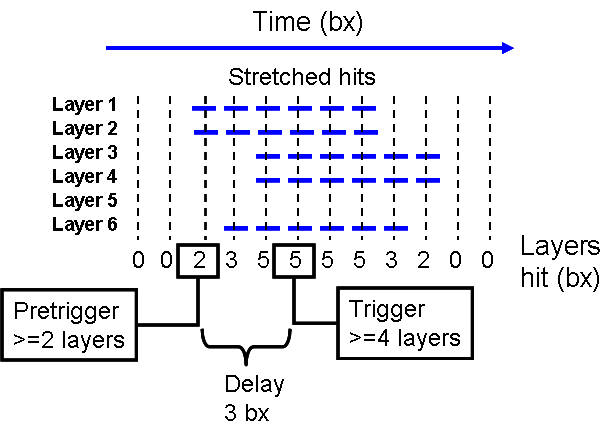
\includegraphics[width=0.73\linewidth]{figures/anode_stretched_hits.png}
                \caption{Anode stretched hits}
                \label{fig:anode_stretched_hits}
        \end{center}
\end{figure}

Each pattern detector can detect a programmable "collision" pattern as well as a fixed "accelerator" pattern. The input data for the collision pattern detector are selected as shown below:

\begin{center}
\begin{verbatim}
...n-2 n-1 n...........Layer 1
.......n-1 n...........Layer 2
...........n...........Layer 3
...........n n+1.......Layer 4
...........n n+1 n+2...Layer 5
...........n n+1 n+2...Layer 6
\end{verbatim}
\end{center}

where n in this diagram is the key wire group number, which this particular pattern detector is searching the patterns for. The programming of the programmable collision pattern is implemented as a simple masking-out of the bits that we do not want to include in the pattern. The accelerator pattern is a vertical pattern of 6 layers all with strip n only.

Each ALCT candidate is assigned a quality equal to number of layers with hits minus 3 and passes through a ghost cancellation procedure: it is cancelled if there is another ALCT candidate at the same bunch crossing in the previous wirewith the same or better quality or in the next wire with better quality, or if there is ALCT candidate up to 4 bunch crossing clocks earlier with any quality.

In each bunch crossing two ALCTs with highest quality are sent to the TMB (Trigger MotherBoard), which requires a coincidence between anode and cathode trigger information. In the case of a Level-1 Accept signal from the Global Trigger (distributed via the TTC system to the CCB in each peripheral crate), ALCT data are sequentially transmitted to the Trigger Mother Board and hence to the DAQ Motherboard. These data frames include a few words of ALCT trigger data and a much larger amount of ALCT raw hit data consisting of a time sequence of raw CSC anode wire-group hits that have been stored at the 40 MHz bunch crossing frequence by the ALCT2001. Typically 8 to 16 bunch crossings are read out for each wire group. FIFO data can also be read out much more slowly through VME access via the TMB board using a JTAG electrical interface to the ALCT, if necessary.

For self-monitoring and also for powering and controlling the AFEB cards, the ALCT contains a Slow Control section that supplies power to the AFEBs, controls AFEB thresholds, provides and controls the amplitude of test pulses to the AFEBs, and reads back power supply voltages and currents, as well as on-board temperature. 

\newpage
\subsection{Software Emulation of ALCT Processing}

ALCT processing includes the following five steps:

\begin{itemize}
    \item Pulse extension;
    \item Pretrigger;
    \item Trigger;
    \item Ghost cancellation;
    \item ALCT construction.
\end{itemize}

\subsubsection{Pulse Extension}

Sofware emulation provides information about all wire signals in DAQ readout window (16 BXs). A search for these signals is performed in a loop over all wire groups, all layers, and all 16 BXs; found signals are stretched over 6 BXs (see Fig.~\ref{fig:alct_pulse_extension}).

\begin{figure}[tbh]
        \begin{center}
                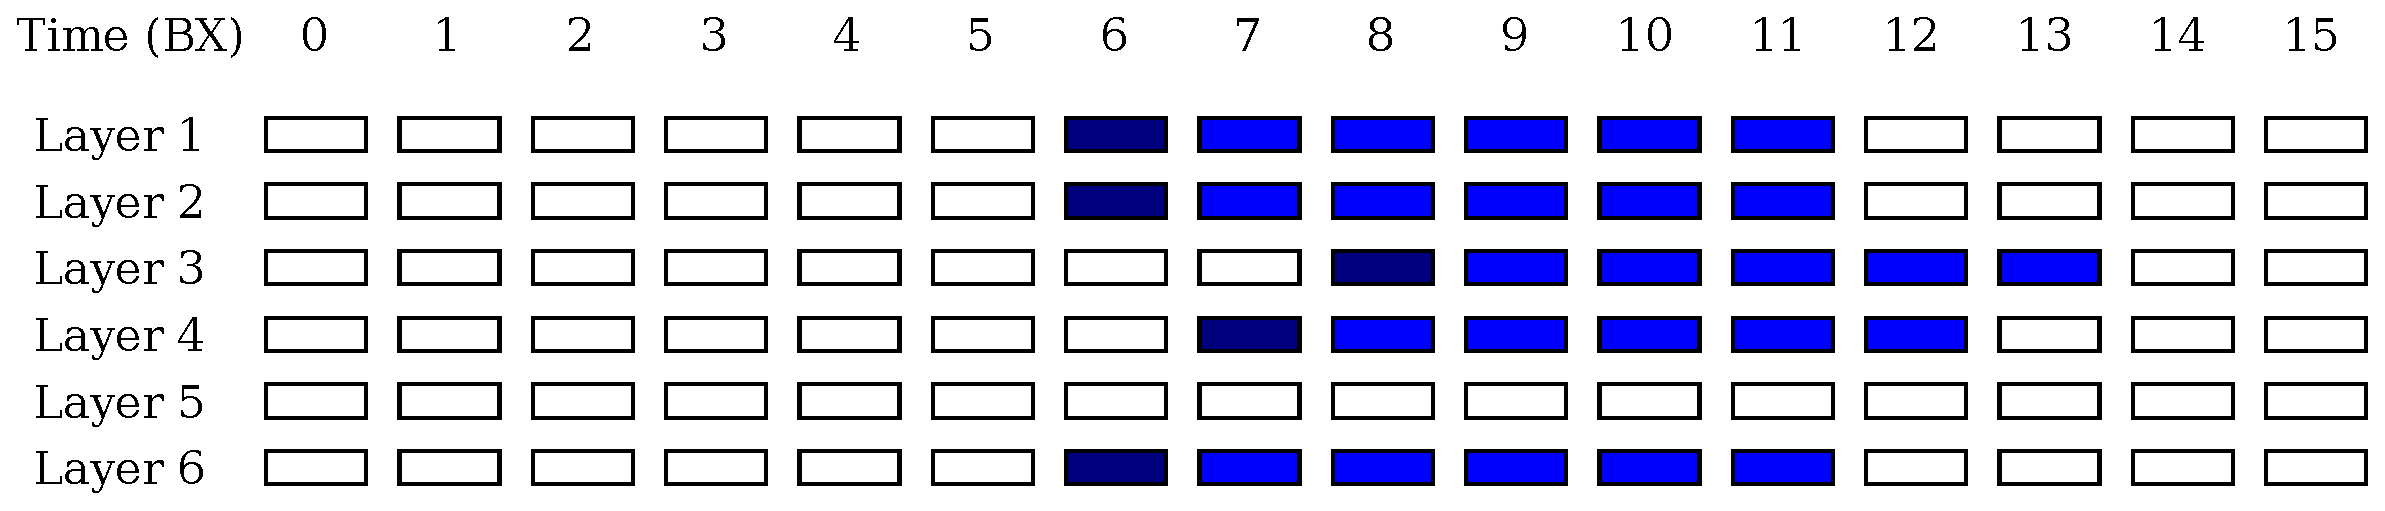
\includegraphics[width=0.9\linewidth]{figures/stretched_hits_alct.pdf}
                \caption{Illustration of ALCT pulse extension for one specific wire group.}
                \label{fig:alct_pulse_extension}
        \end{center}
\end{figure}

\subsubsection{Pretrigger}

After all available wire signals are stretched, a search for ALCT pretriggers is performed in all wire groups and all BXs. For any given wire group and BX, we count the number of layers with hits within the pattern mask shown on Fig.~\ref{fig:alct_pretrigger}, and if this number is greater than or equal to three, then we say that a pretrigger occured in this wire group and BX. The search for next ALCT pretrigger starts 6 BXs later.

\begin{figure}[tbh]
        \begin{center}
                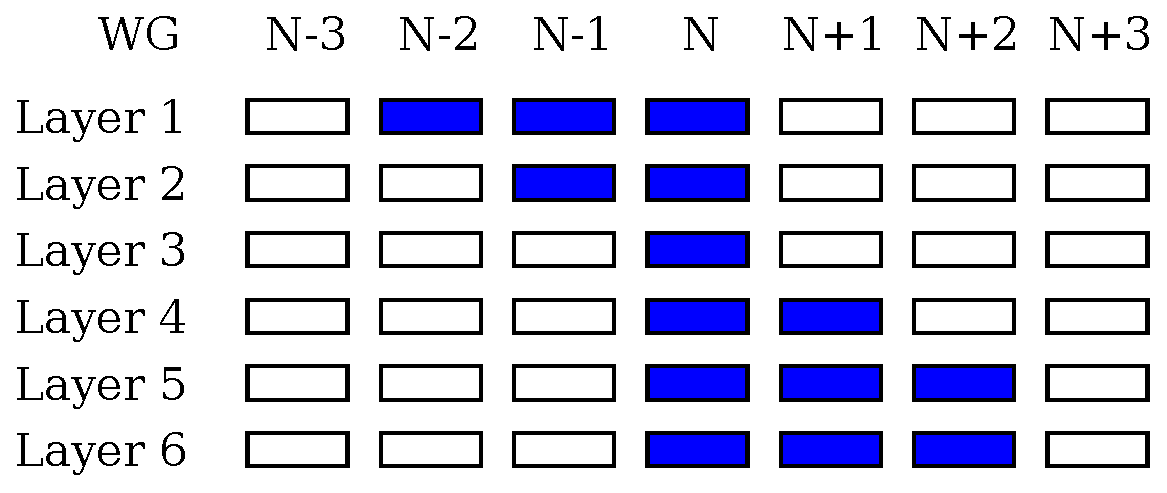
\includegraphics[width=0.45\linewidth]{figures/alct_pretrigger.pdf}
                \caption{ALCT pattern mask for pretriggering and triggering.}
                \label{fig:alct_pretrigger}
        \end{center}
\end{figure}

\subsubsection{Trigger}

After all ALCT pretriggers are found, for each pretrigger in BX = B we check for a trigger in BX = B+2. For any given wire group and BX = B+2, we count the number of layers with hits within the same pattern mask used for pretriggering, and if this number is greater than or equal to four, we say that a pretrigger occured in this wire group and BX, and assign it a quality Q = number of layers with hits-3. If in some wire group more than one trigger occured, we report only the one with the highest quality. If there are two triggers with the same quality, report the earlier one.

\subsubsection{Ghost Cancellation}

Not all triggers found in the previous step are used to construct ALCTs: before that all of them pass through so called ghost cancellation procedure.

A trigger in wire group = N and BX = B is cancelled if there is a trigger in wire group = N-1:
\begin{itemize}
    \item either in the same BX = B and with better or equal quality;
    \item or to 4 BXs earlier, with any quality.
\end{itemize}

In addition, a trigger in wire group = N and BX = B is cancelled if there is a trigger in wire group = N+1:
\begin{itemize}
    \item either in the same BX = B and with better quality;
    \item or to 4 BXs earlier, with any quality.
\end{itemize}

\subsubsection{ALCT Construction}

Construct ALCTs from triggers survived after the ghost cancellation procedure: encode quality, WG, BX (defined by pretrigger BX). In every BX choose best two ALCTs: two ALCTs with the highest quality. If we need to choose one ALCT from two ALCTs with the same quality: choose the one with larger wire group.

\newpage
\subsection{CLCT Processing}

[We need a good picture illustrating CLCT processing process like in the case of ALCT one]

A muon passing through a CSC chamber will produce distinctive patterns of half-strip
hits in the six-layer endcap muon CSC chambers. By identifying these patterns, the CSC Local
Trigger provides high rejection power against backgrounds. The largest background source,
neutron-induced gamma ray conversions, are generally low in energy, and produce mostly single-
layer or short multi-layer hits. Other backgrounds, such as low-momentum muons or punch-
through particles often do not point well enough to the primary interaction region to be considered
high-momentum muon candidates.

\begin{figure}[tbh]
        \begin{center}
                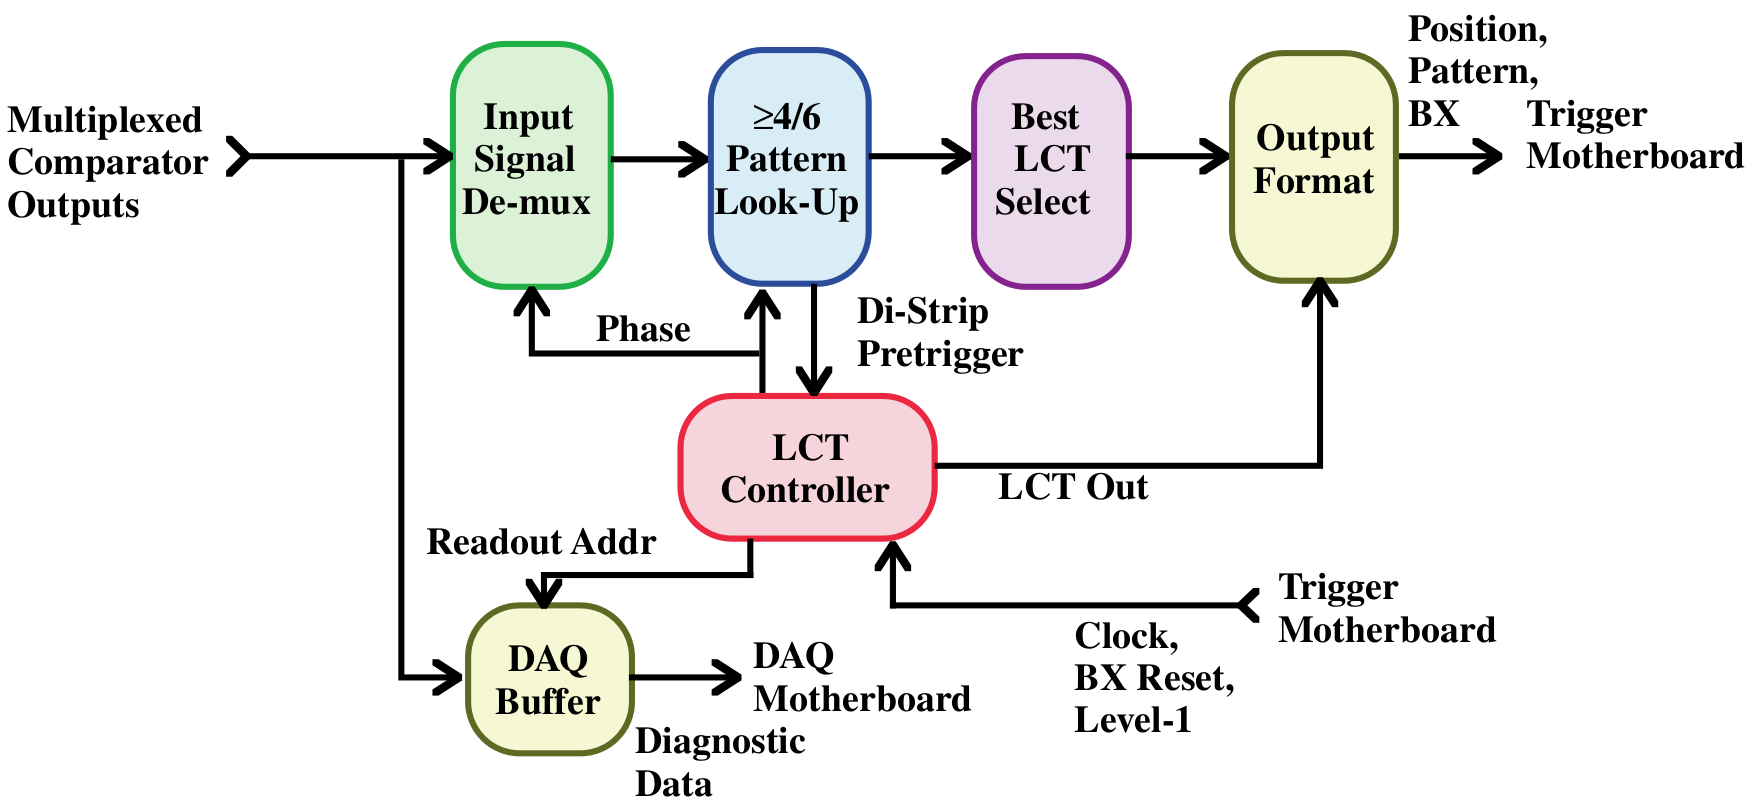
\includegraphics[width=0.73\linewidth]{figures/CLCT_block_diagram.png}
                \caption{CLCT block diagram}
                \label{fig:clct_block_diagram}
        \end{center}
\end{figure}

[Technical description from TMB manual below]

For each of 160 key half-strips consider the 42 neighboring half-strips (i.e. on key 5 use the following half-strips):

\begin{figure}[tbh]
        \begin{center}
                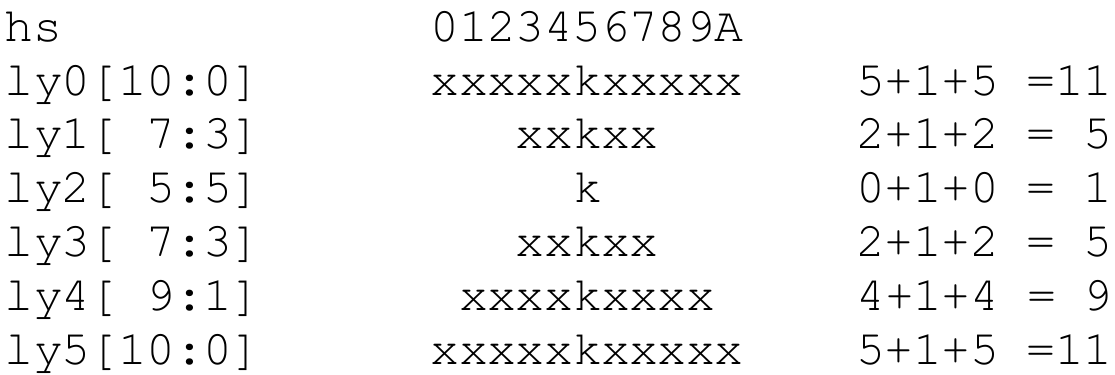
\includegraphics[width=0.48\linewidth]{figures/160_key_half_strips.png}
                \caption{160 key half-strips}
                \label{fig:160_key_half_strips}
        \end{center}
\end{figure}

For each of 160 key half-strips, count layers with hits matching the 9 pattern templates:

\begin{figure}[tbh]
        \begin{center}
                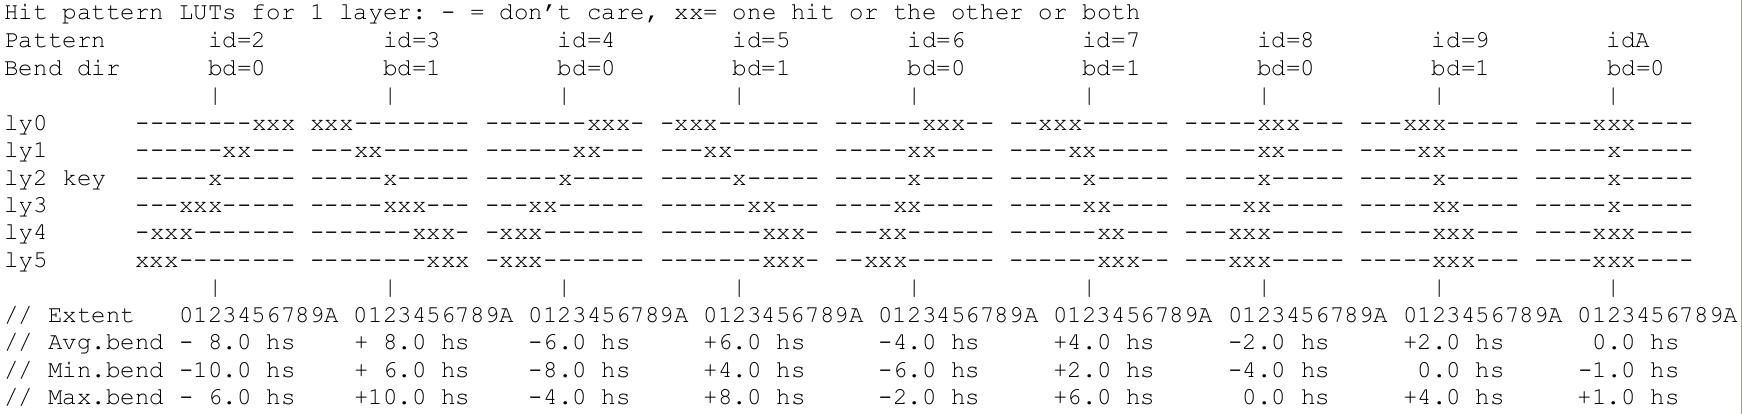
\includegraphics[width=0.98\linewidth]{figures/CLCT_patterns.png}
                \caption{CLCT patterns}
                \label{fig:clct_patterns}
        \end{center}
\end{figure}

Pattern ID=1 is a layer-OR trigger, Pattern ID=0 is no-pattern-found. Result for each of 160 keys is a list of 9 pattern-ID numbers (pid) [2 to A] and corresponding
number of layers [0 to 6] with matching hits (nhits). Find the best 1-of-9 pattern ID numbers for each key by comparing nhits. Ignore bend direction: left and right bends have equal priority (bit 0 of pid implies bend direction).
If two pattern IDs have the same nhits, take the higher pattern ID. A key with no matching hits, would always return pid=A and nhits=0.
Pre-trigger if any 1-of-160 keys have nhits $\geq$ hit\_thresh\_pretrig and pid $\geq$ pid\_thresh\_pretrig.

Construct 7-bit pattern quality pat[7:0] for sorting where pat[7:5]=nhits[2:0], pat[4:0]=pid[3:0]. Ignore the bend direction bit (pid[0]), left and right bends have equal priority. 
Store pat[7:0] for 160 keys for use later to find 2nd CLCT.
Find the best key out 1-of-160 keys by sorting on the 6-bit number pat[7:1]. Store 1st CLCT info: key, pattern ID, and number of hits.
For empty events, key=0, pid=A and nhits=0. If clct\_blanking=1, then key=pid=hits=0.

Mark keys near 1st CLCT as busy from 1st key-nspan to 1st key+pspan.
If clct\_sep\_src=1, pspan and nspan are set equal to clct\_sep\_vme, typically 10 half-strips.
If clct\_sep\_src=0, pspan and nspan are read from RAM and depend on the pattern ID number, this allows two less bending tracks to be closer than more bending tracks.

Find the best key out of 1-of-160 keys by sorting on the 6-bit number pat[7:1]: skip busy keys, if two keys have the same pat[7:1] take the lower key.
Store the same information for the 2nd CLCT as for the 1st one.

Wait for CSC drifting (drift delay of 2BXs) and perform matching to ALCTs.

\newpage
\subsection{Software Emulation of CLCT Processing}

CLCT processing includes the following four steps:

\begin{itemize}
    \item Pulse extension;
    \item Pretrigger;
    \item Trigger;
    \item CLCT construction and CLCT dead time.
\end{itemize}

In contrast to ALCT processing, where all steps are independent and performed one after another for all 16 BXs, during CLCT processing last three steps repeated in one global loop over BXs.

\subsubsection{Pulse Extension}

Sofware emulation provides information about all half-strip signals in DAQ readout window (16 BXs). A search for these signals is performed in a loop over all half-strips, all layers, and all 16 BXs; found signals are stretched over 6 BXs (see Fig.~\ref{fig:clct_pulse_extension}).

\begin{figure}[tbh]
        \begin{center}
                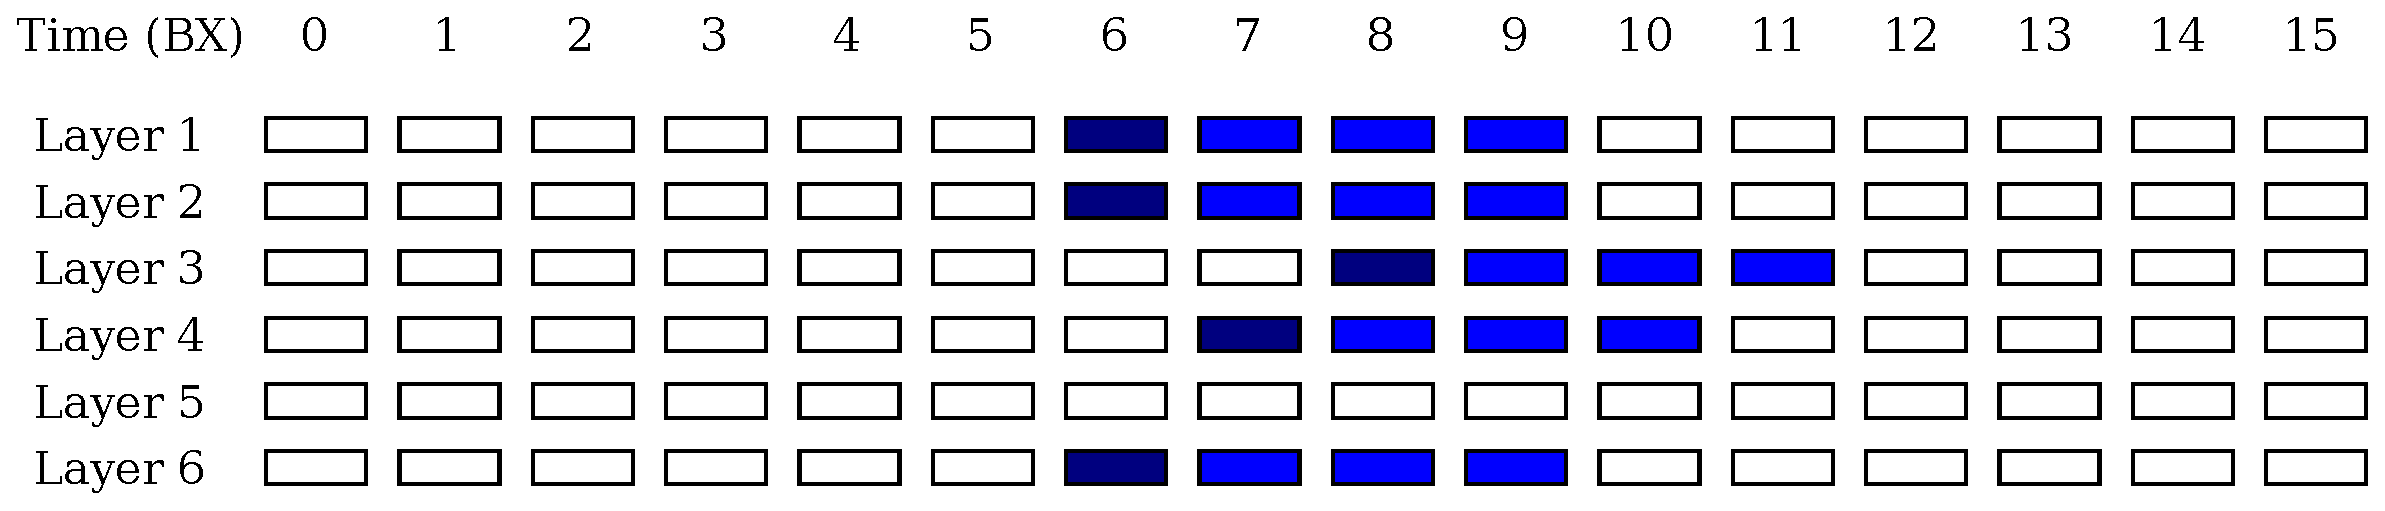
\includegraphics[width=0.9\linewidth]{figures/stretched_hits_clct.pdf}
                \caption{Illustration of ALCT pulse extension for one specific half-strip.}
                \label{fig:clct_pulse_extension}
        \end{center}
\end{figure}

\subsubsection{Pretrigger}

After all available half-strip signals are stretched, start a global loop over all BXs from BX = 0 and search for CLCT pretriggers in all half-strips. For any given BX and half-strip, count the number of layers with hits within the patterns shown on Fig.~\ref{fig:clct_pretrigger}, and if this number is greater than or equal to three, then we say that a pretrigger occured in this BX and this half-strip. This pretrigger is only accepted if its pattern id $\geq$ 2. If there were no CLCTs found in some BX = B, proceed to BX = B+1 and continue searching for pretriggers. If there are some CLCTs found in the current BX, proceed to next step.

\begin{figure}[tbh]
        \begin{center}
                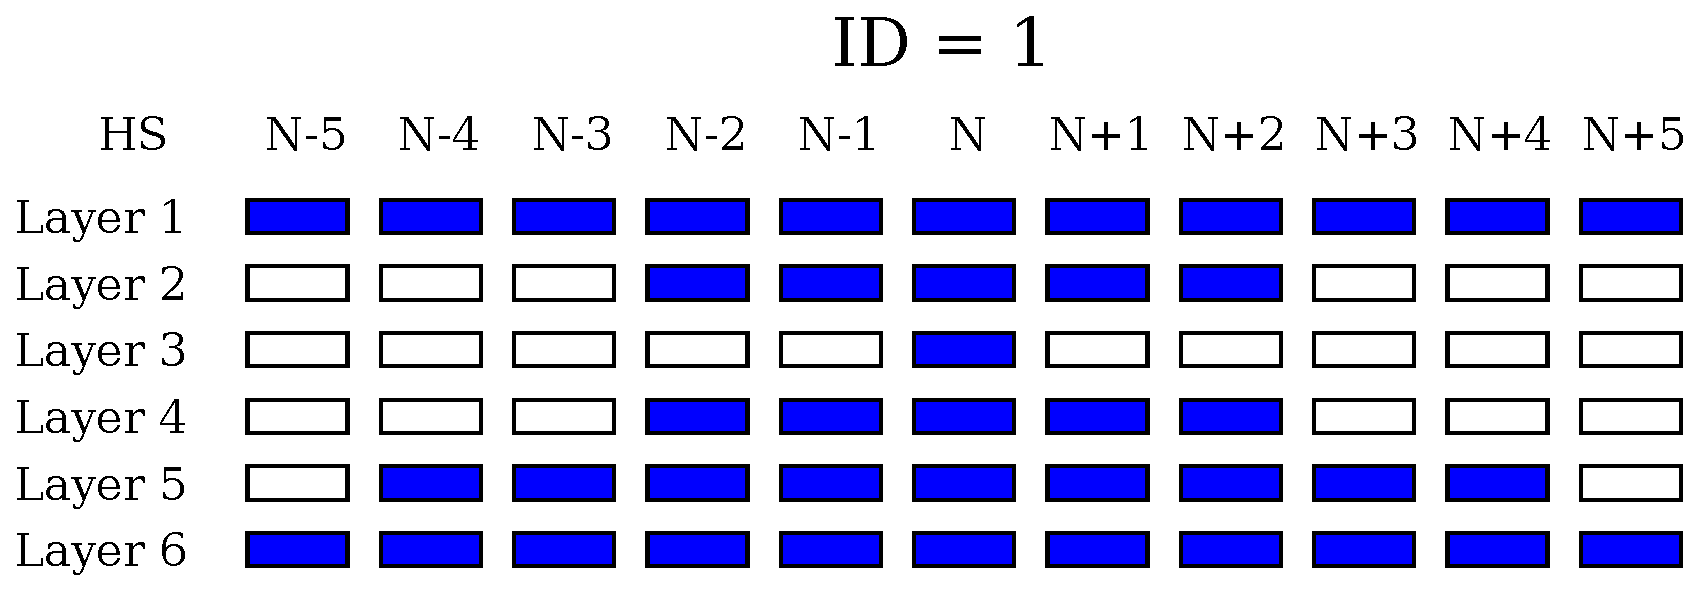
\includegraphics[width=0.48\linewidth]{figures/clct_pattern_01.pdf}
                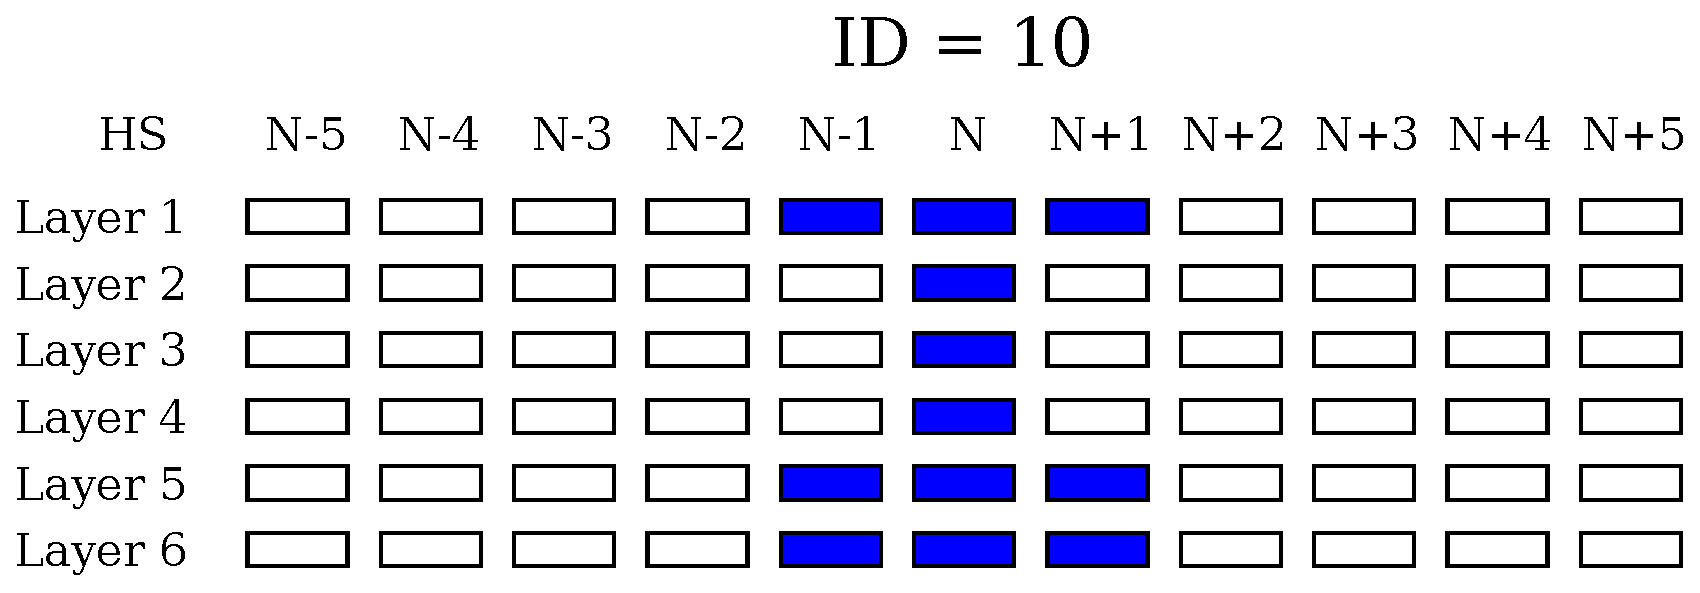
\includegraphics[width=0.48\linewidth]{figures/clct_pattern_10.pdf}\\
                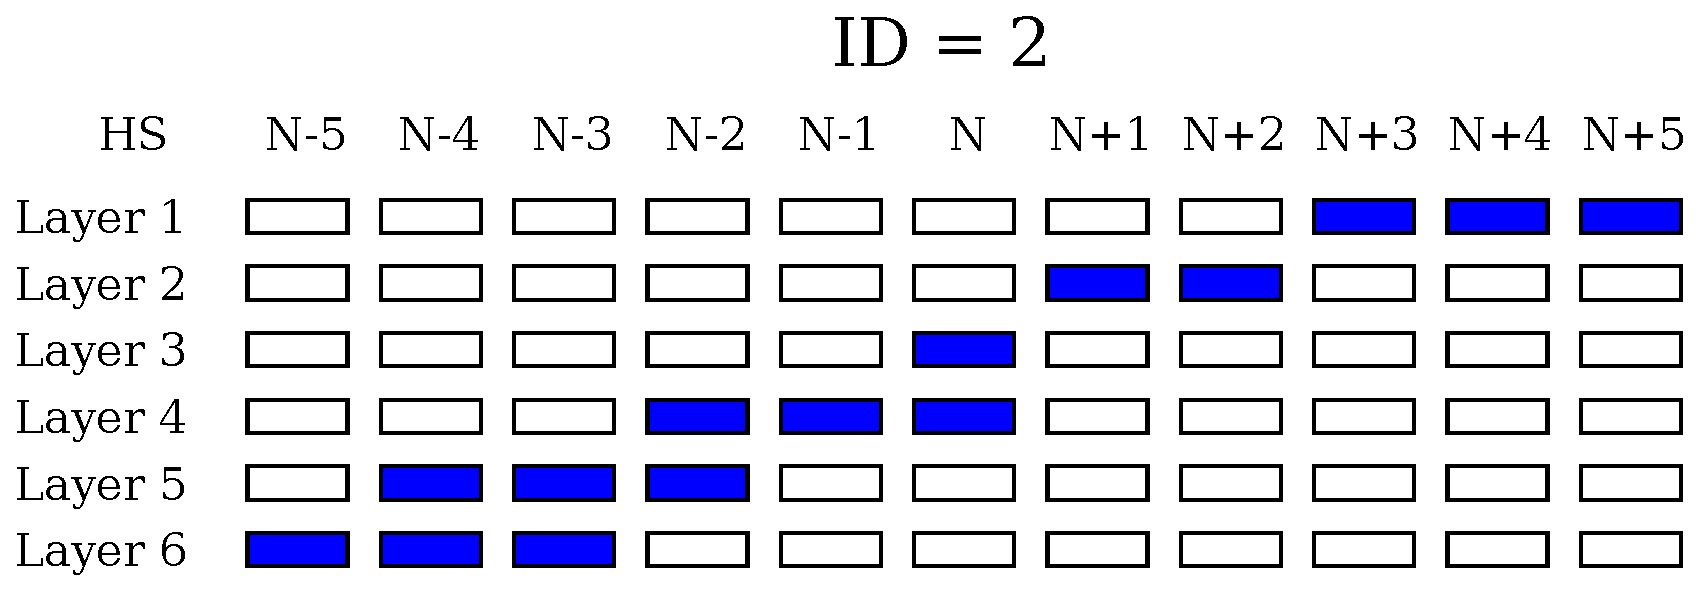
\includegraphics[width=0.48\linewidth]{figures/clct_pattern_02.pdf}
                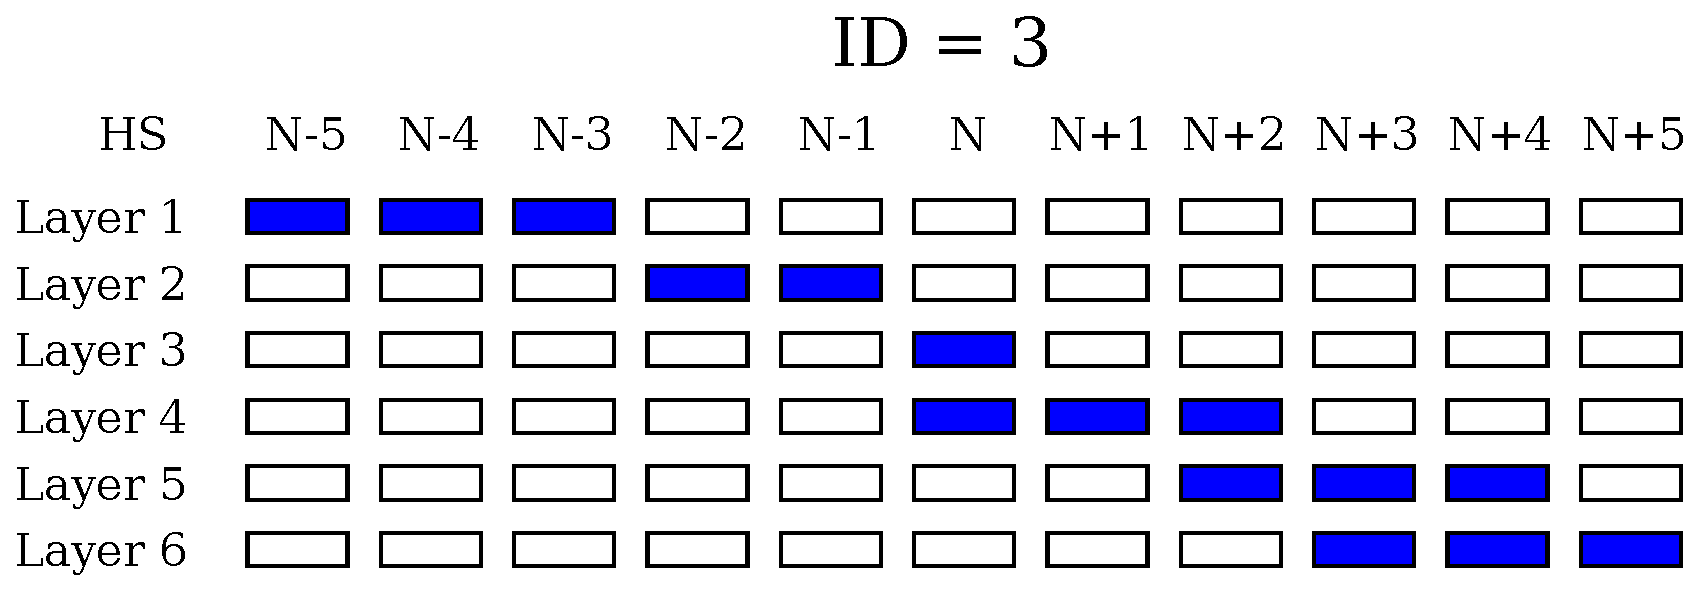
\includegraphics[width=0.48\linewidth]{figures/clct_pattern_03.pdf}\\
                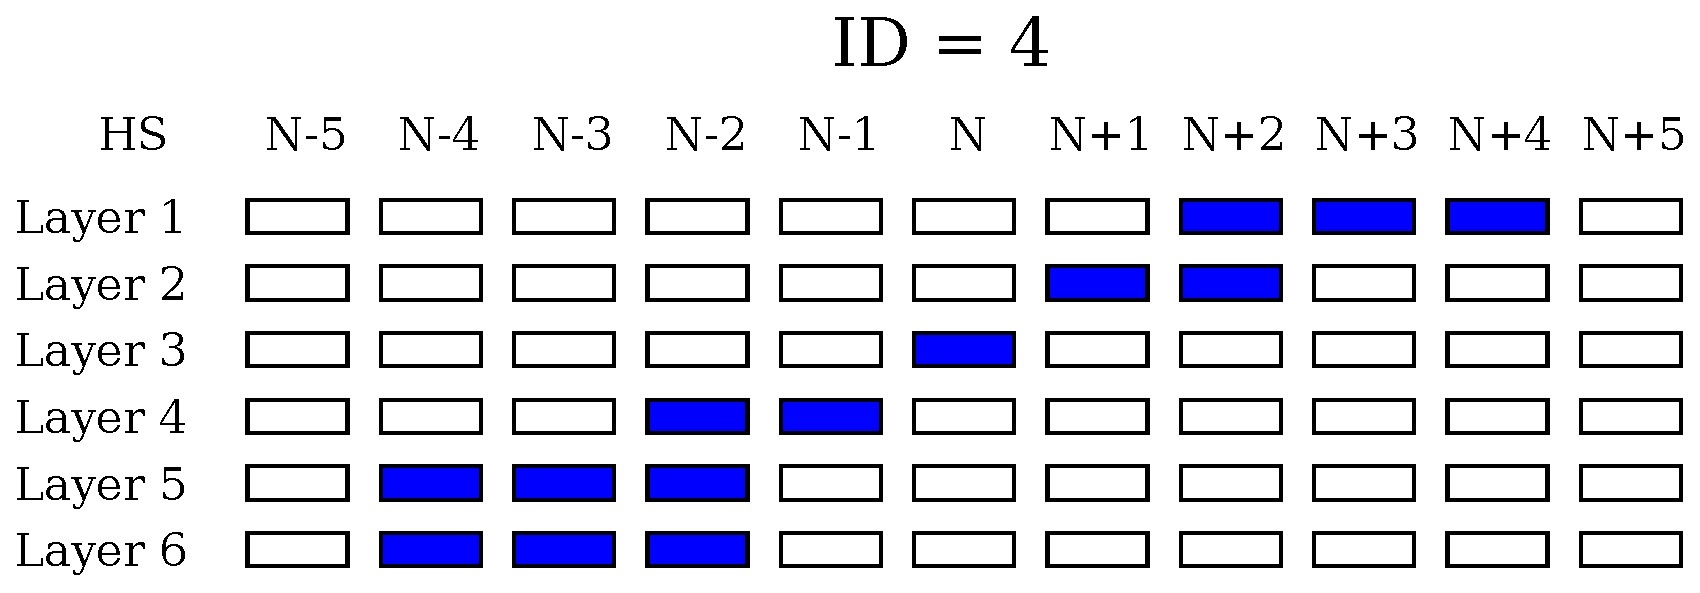
\includegraphics[width=0.48\linewidth]{figures/clct_pattern_04.pdf}
                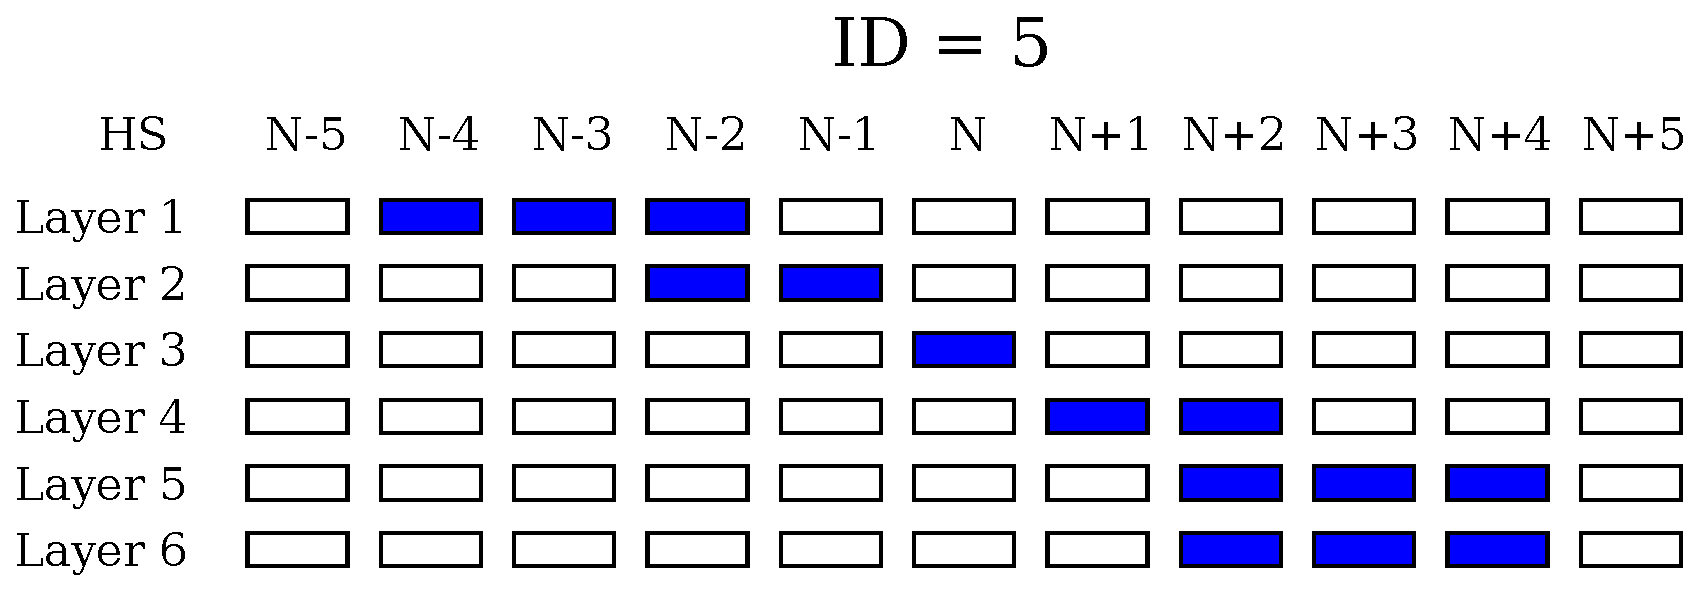
\includegraphics[width=0.48\linewidth]{figures/clct_pattern_05.pdf}\\
                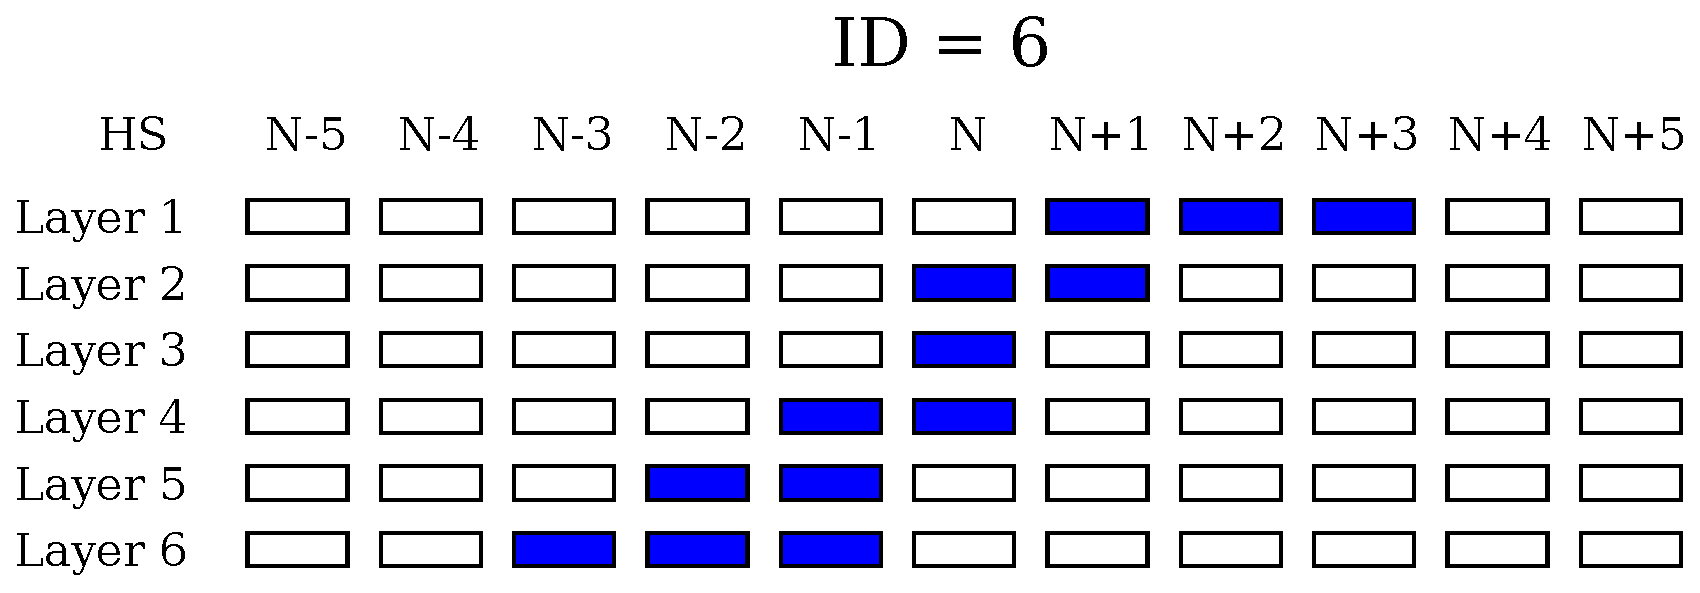
\includegraphics[width=0.48\linewidth]{figures/clct_pattern_06.pdf}
                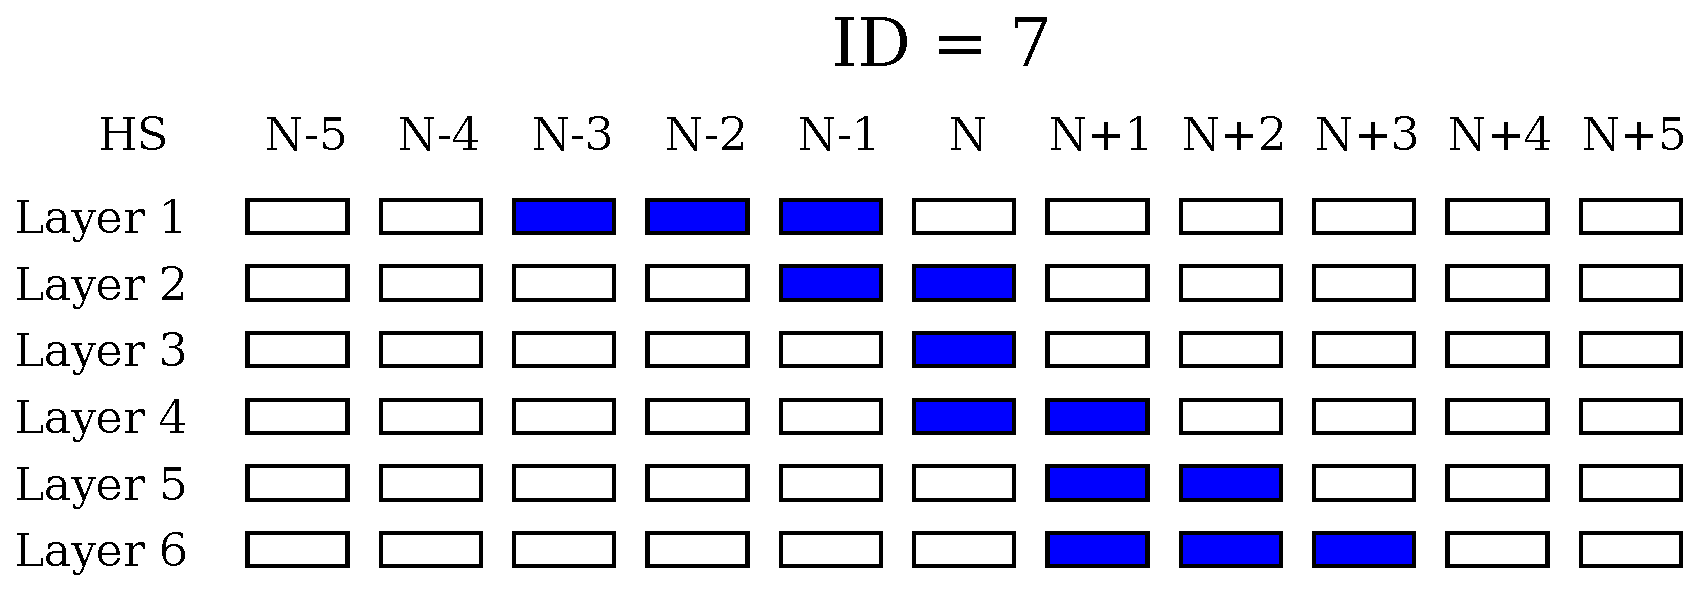
\includegraphics[width=0.48\linewidth]{figures/clct_pattern_07.pdf}\\
                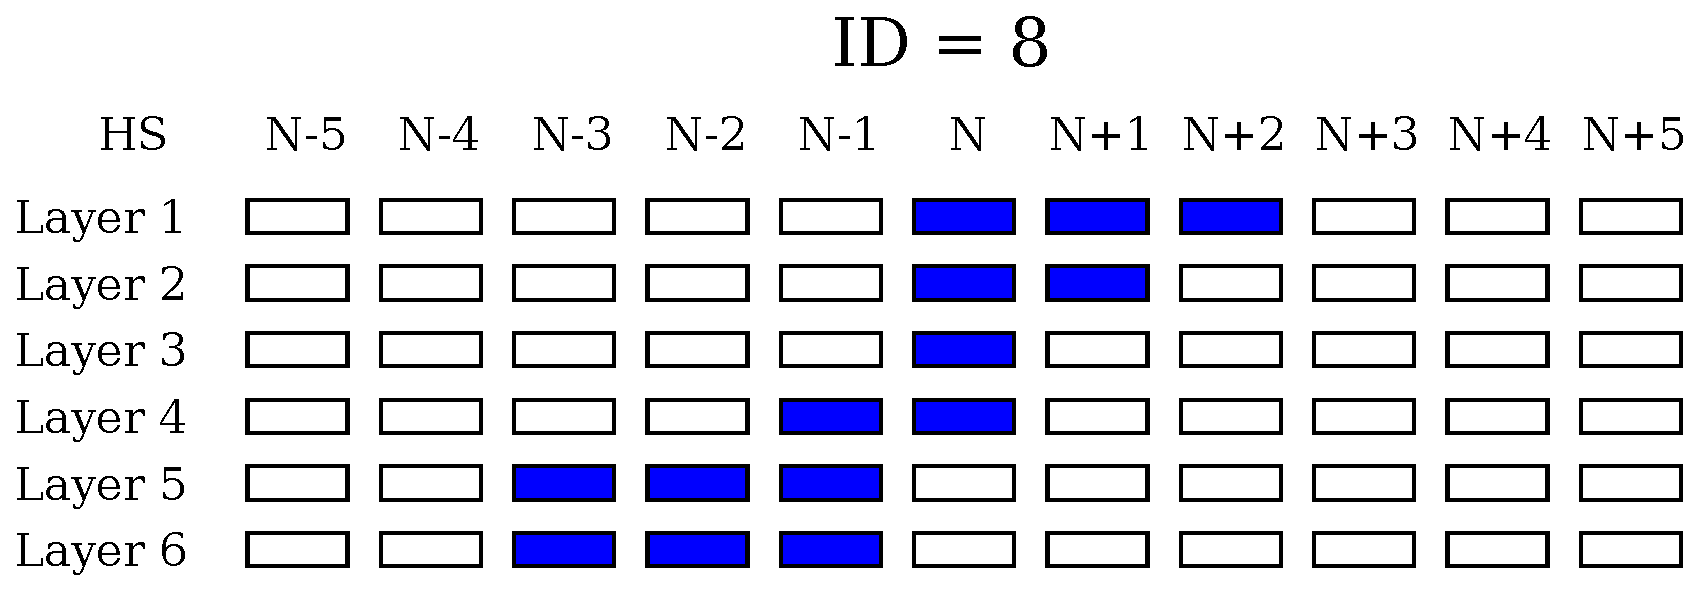
\includegraphics[width=0.48\linewidth]{figures/clct_pattern_08.pdf}
                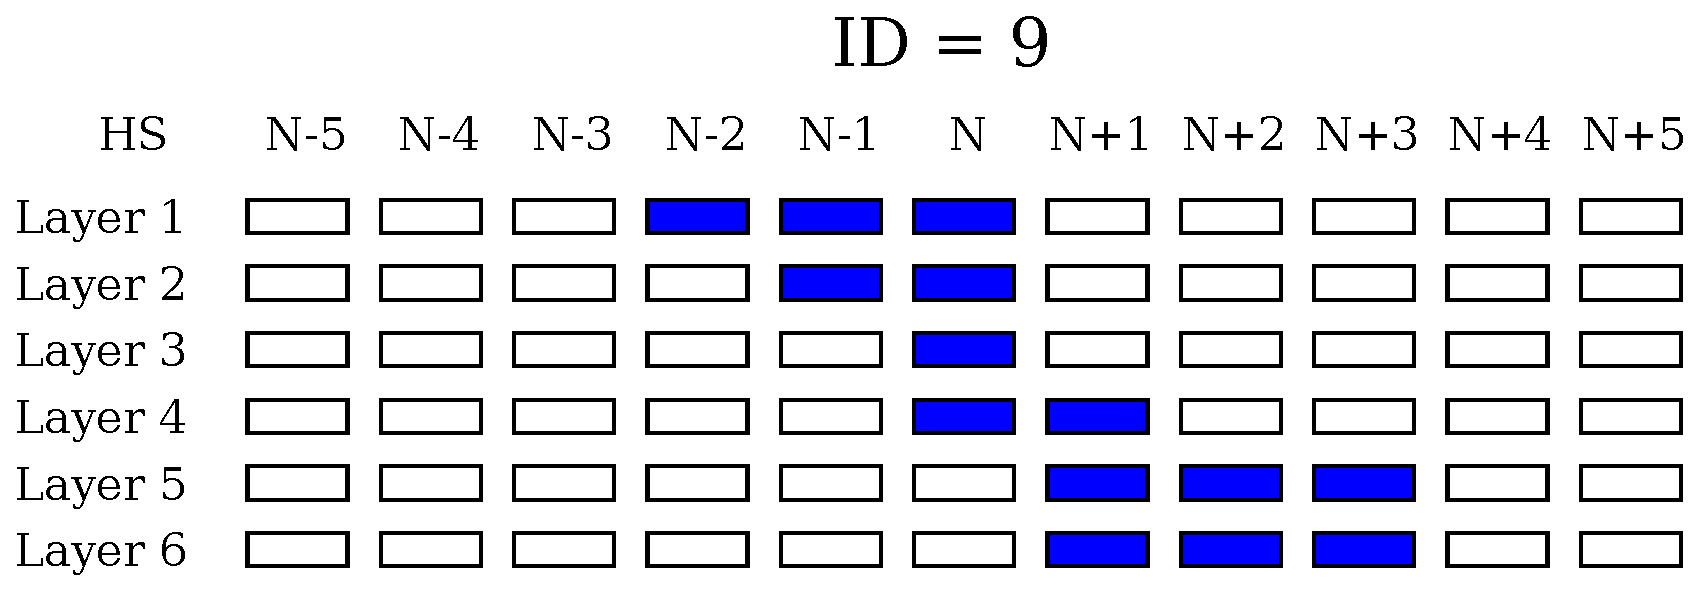
\includegraphics[width=0.48\linewidth]{figures/clct_pattern_09.pdf}
                \caption{CLCT patterns for pretriggering and triggering.}
                \label{fig:clct_pretrigger}
        \end{center}
\end{figure}

\subsubsection{Trigger}

As soon as a BX = B with CLCT pretrigger(s) is found, search for triggers in BX = B+2. For each half-strip, count the number of layers with hits within the same patterns used for pretriggering, and if this number is greater than or equal to four, we say that a trigger occured in this half-strip and BX, and remember:
\begin{itemize}
    \item pattern id with the highest number of hit layers (if there are two pattern ids with the same number of hit layers, choose smaller pattern id);
    \item number of hit layers in this pattern id.
\end{itemize}

Proceed to next step.

\subsubsection{CLCT Construction and CLCT Dead Time}

In a BX with CLCT triggers, find up to two best triggers to be used in CLCT construction.

Find the best trigger:
\begin{itemize}
    \item Find trigger with the highest number of hit layers;
    \item If there are two triggers with the same number of hit layers: choose the one with higher pattern id;
    \item If there are two triggers with the same number of hit layers and the same pattern id: choose the one with smaller half-strip.
\end{itemize}

Mark zone of 20 half-strips around the best trigger as used and find the second best trigger among not used half-strips.

Construct up to two best CLCTs from found best triggers: encode quality, pattern, bending direction, half-strip, cfeb, BX (defined by pretrigger BX).

After CLCT construction, keep CLCT "dead": continue the loop over all BXs until there is a BX with no triggers. When such a BX is found go back to pretriggering step.

\newpage
\subsection{CLCT and ALCT Correlation}

The Trigger Motherboard (TMB) portion of the CLCT/TMB card receives up to two
anode stubs from the ALCT board and two cathode stubs from the CLCT portion of the CLCT/
TMB card. The functions of the TMB circuitry are:

\begin{itemize}
	\item Bunch crossing alignment of the anode and cathode tags.
	\item Correlation of the Anode and Cathode LCT words and construction of two combined LCTs.
	\item Transmission of LCT data to the Muon Port Card (MPC) for triggering, and transmission of DAQ data to the DAQ Motherboard (DAQMB).
\end{itemize}

Incoming anode and cathode LCTs are not aligned in time. Anode LCTs are created
faster than cathode LCTs because of the slow development of the cathode preamp signal, and
because processing inside the ALCT card is faster than processing inside the CLCT logic. The
TMB contains input pipeline logic in order to delay anode LCTs for a programmable number of
bunch crossings up to 10.

The anode and cathode LCTs are matched according to the more precise ALCT bunch
crossing number (BXN). The Cathode LCT BXN can differ by at most $\pm$1 bunch crossing. For each
of the selected muons the TMB outputs a 2-bit bunch crossing match word as shown in
table below. These may be used by later boards in the trigger chain if additional quality information
is needed. They also allow the analysis of the bunch crossing matching in the TMB, since a large
number of bad matches could be an indication of a timing alignment problem.

The ideal case for a high-momentum muon is one anode and one cathode LCT pattern.
However, other cases may occur, which are distinguished by a 2-bit “STA” (Status type A) code:

\begin{itemize}
	\item The TMB may receive one or two anode LCTs and zero cathode LCT patterns. This
happens, for example, for very low-momentum muons. Although the non-zero data is
forwarded to the MPC, this case is flagged by STA=1, as is the similar case of one or two
cathode LCT and zero anode LCT patterns.
	\item If the TMB receives two anode LCTs and one cathode LCT, the TMB outputs two LCTs,
by copying the Cathode LCT bits into both muons. These, and the similar case of two
cathode LCTs and one anode LCT, are flagged by STA=2.
	\item If there are two anode LCTs and two cathode LCTs in one chamber, they are matched
according to their pattern numbers: the largest ALCT and CLCT pattern numbers are
paired, and the second largest ALCT and CLCT pattern numbers are paired. These, and
the ideal case of a single match, are flagged by STA=3.
\end{itemize}

TMBs maintain a local Bunch Crossing Number (BXN) using signals from the Clock
and Control Board. The internal BXN is compared to the BXN received from the ALCT module,
and the Sync Error bit is set if a mismatch is detected.

The TMB sends up to two anode LCT and two cathode LCT patterns for one CSC
chamber to the MPC every 25 ns.

\newpage
\subsection{Software Emulation of CLCT and ALCT Correlation}

Every BX OTMB receives up to 2 CLCTs and up to two ALCTs from CLCT and ALCT processors, Fig.~\ref{fig:clcts_alcts} shows an example which will be used throughout the subsection.

\begin{figure}[tbh]
        \begin{center}
                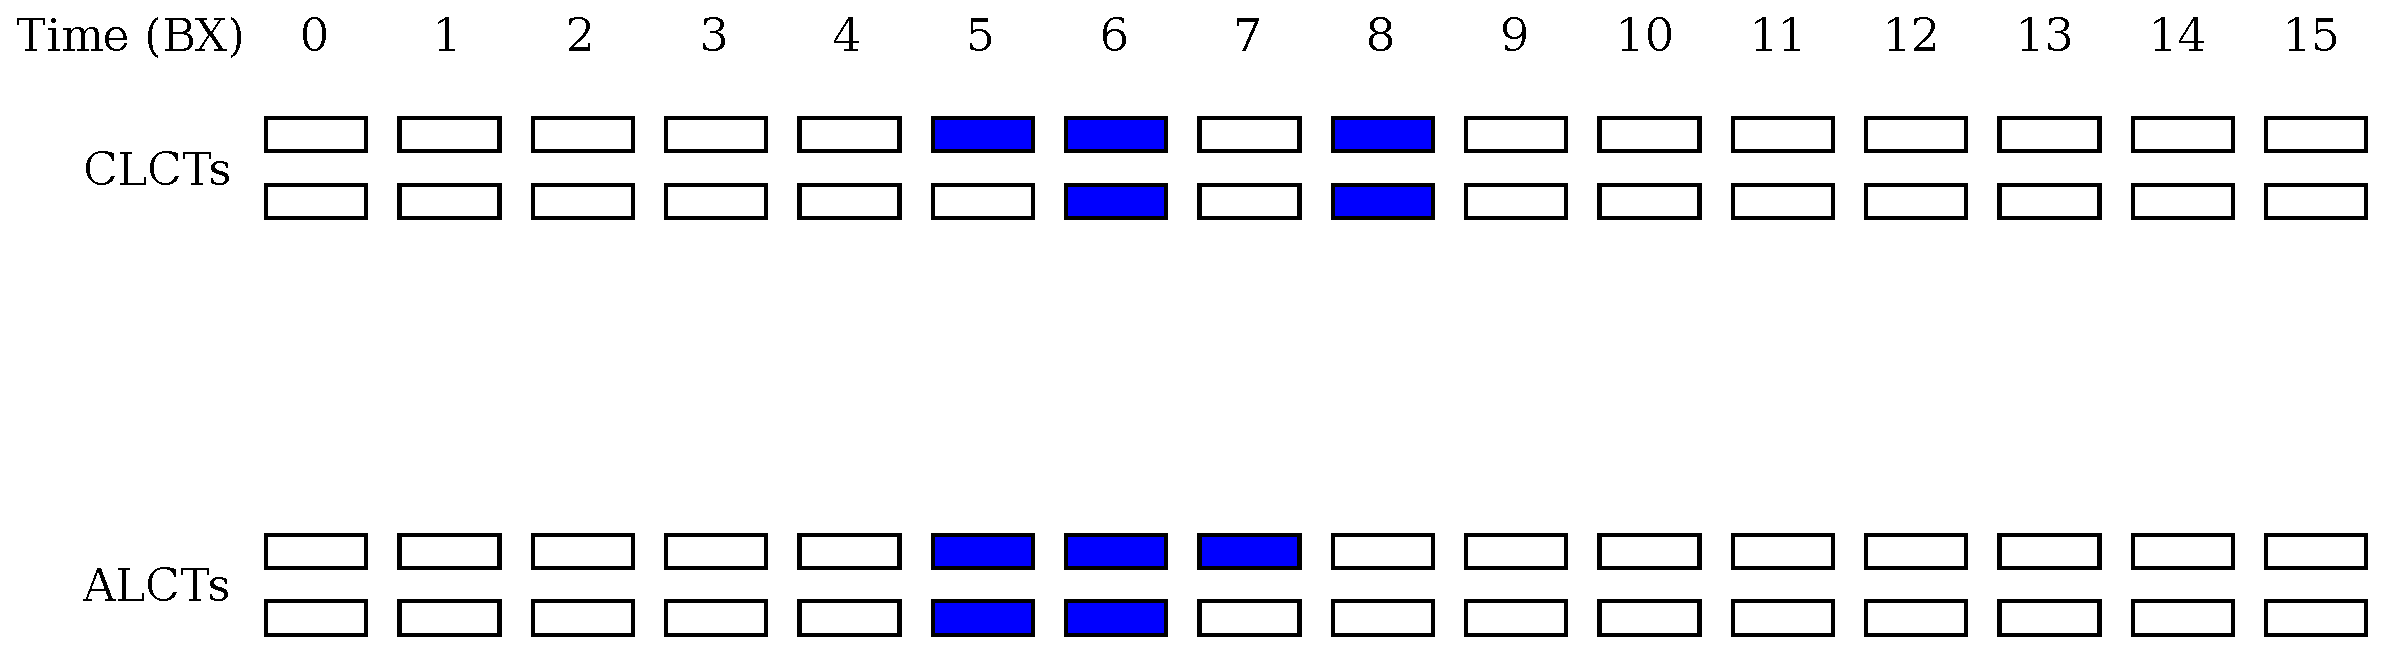
\includegraphics[width=0.7\linewidth]{figures/clcts_alcts.pdf}
                \caption{Example of CLCTs and ALCTs received by OTMB.}
                \label{fig:clcts_alcts}
        \end{center}
\end{figure}

There are two approaches to CLCT and ALCT correlation: CLCT-centric and ALCT-centric. We will introduce the former below and discuss the latter later among OTMB level improvements.

CLCT-centric CLCT and ALCT correlation (see Fig.~\ref{fig:clct_alcts}):
\begin{itemize}
    \item Loop over CLCT BXs from BX = 0 to BX = 15
    \item For CLCT BX = B with at least one valid CLCT:
    \begin{itemize}
        \item Loop over ALCT BXs from BX = B-3 to BX = B+3
        \item Find the first ALCT BX in the matching window with at least one valid ALCT and not marked as used before
        \begin{itemize}
            \item Correlate CLCTs and ALCTs in matching ALCT and CLCT BXs
            \item Mark ALCT BX as used
            \item Proceed to next CLCT BX
        \end{itemize}
    \end{itemize}
\end{itemize}

\begin{figure}[tbh]
        \begin{center}
                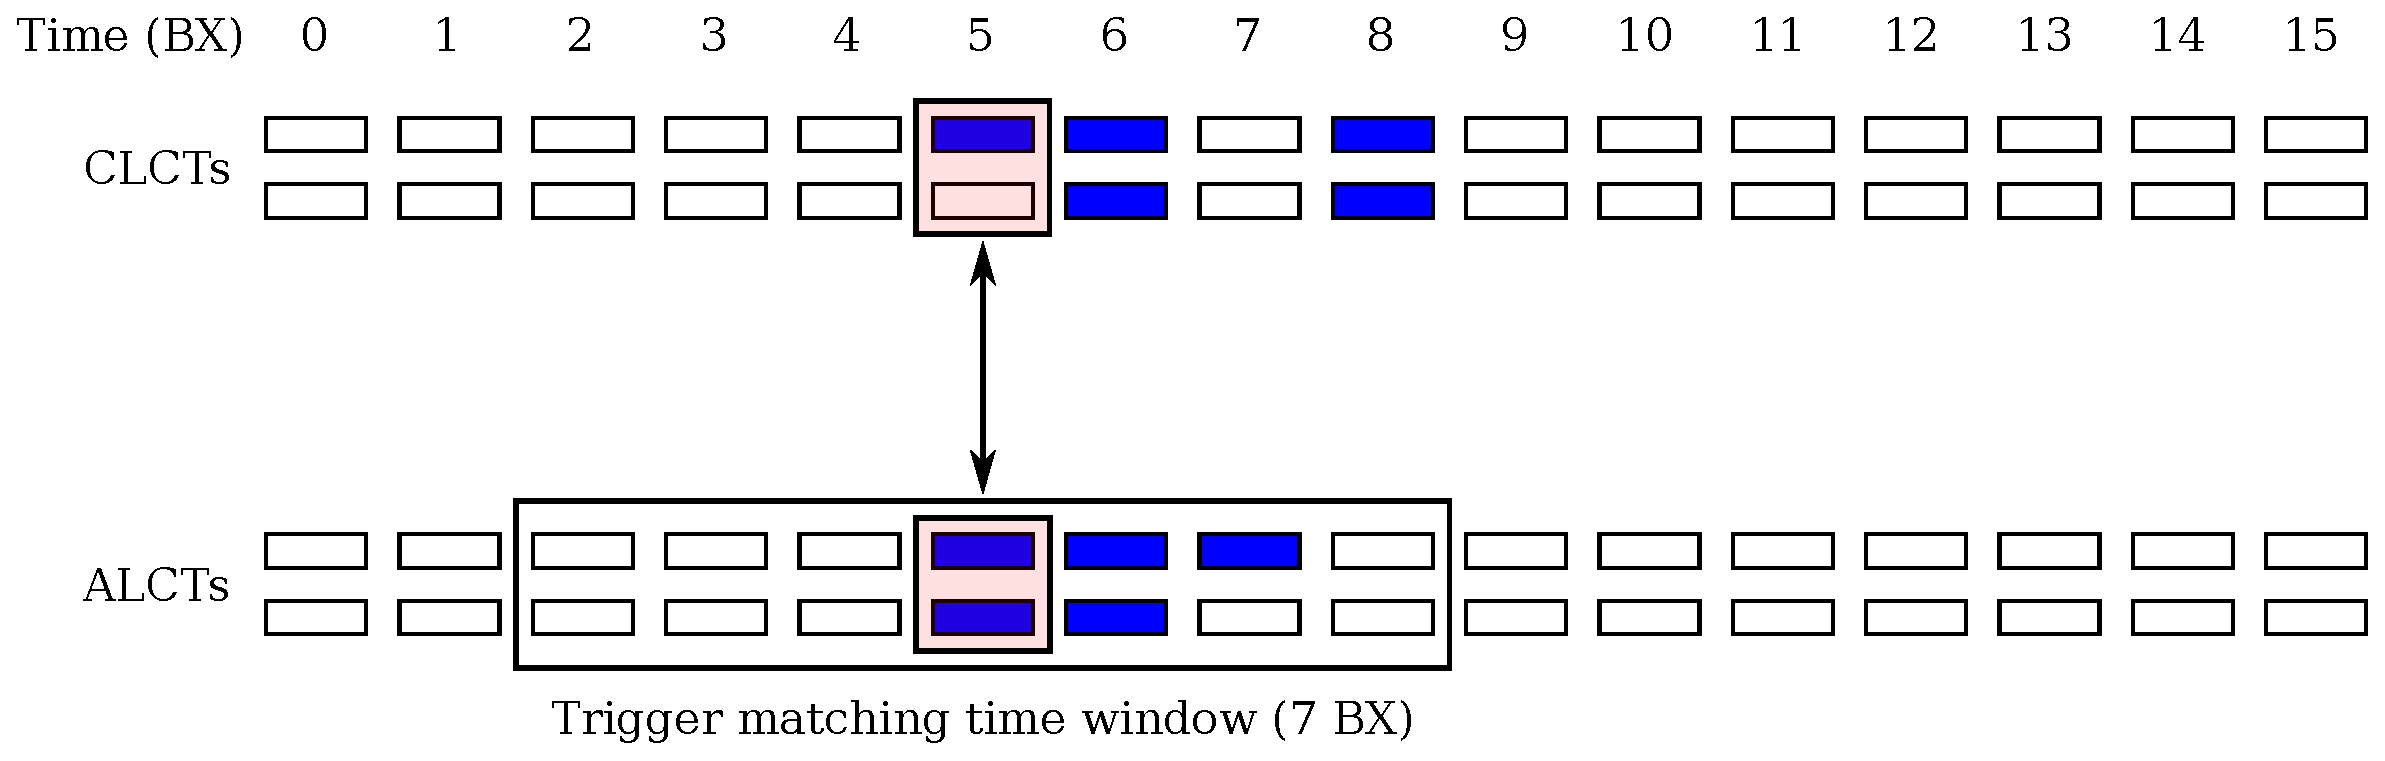
\includegraphics[width=0.7\linewidth]{figures/clct_alcts.pdf}
                \caption{CLCT-centric CLCT and ALCT correlation.}
                \label{fig:clct_alcts}
        \end{center}
\end{figure}

The results of such a correlation are shown on Fig.~\ref{fig:clct_alcts_end}.

\begin{figure}[tbh]
        \begin{center}
                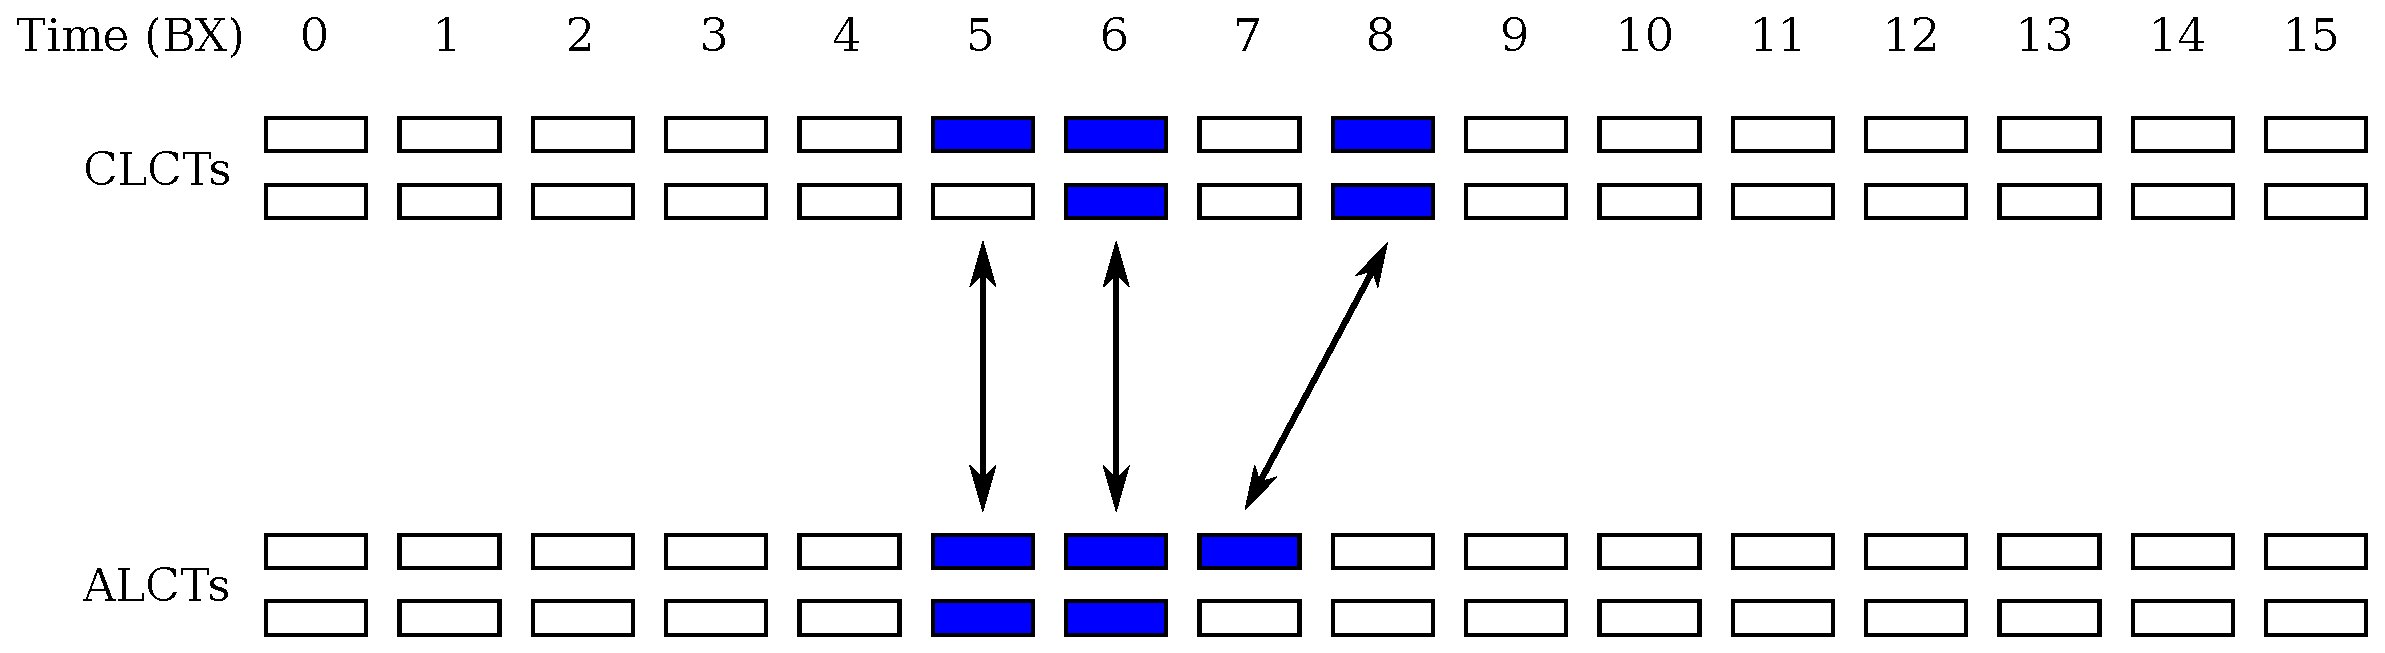
\includegraphics[width=0.7\linewidth]{figures/clct_alcts_end.pdf}
                \caption{Result of CLCT-centric CLCT and ALCT correlation.}
                \label{fig:clct_alcts_end}
        \end{center}
\end{figure}

By default, LCTs are constructed only from valid CLCTs and ALCTs, but we may optionally allow construction of ALCT-less or CLCT-less LCTs.

If there are no ALCT BXs with at least one valid ALCT in the watching window and ALCT-less LCTs are allowed, construct LCTs from valid CLCTs in the current CLCT BX (see example on Fig.~\ref{fig:clct_alcts_alctless} with results on Fig.~\ref{fig:clct_alcts_alctless_end}).

\begin{figure}[tbh]
        \begin{center}
                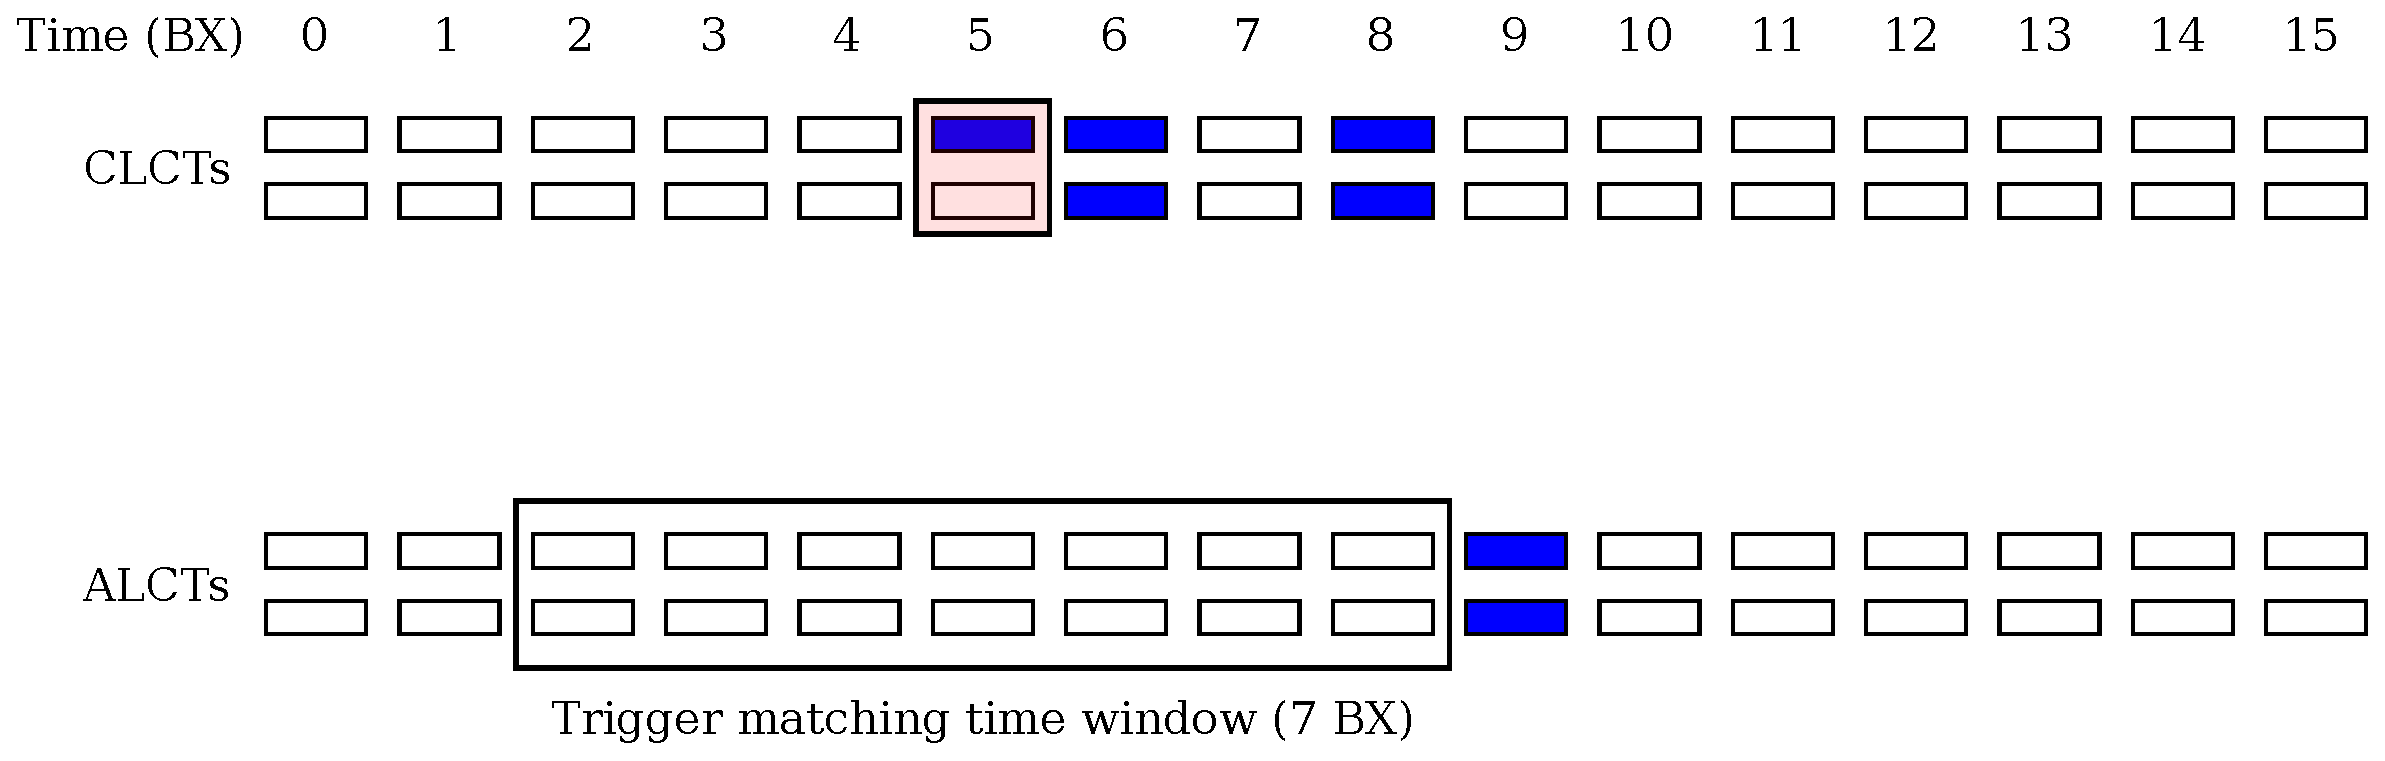
\includegraphics[width=0.7\linewidth]{figures/clct_alcts_alctless.pdf}
                \caption{Example of construction of ALCT-less LCTs.}
                \label{fig:clct_alcts_alctless}
        \end{center}
\end{figure}

\begin{figure}[tbh]
        \begin{center}
                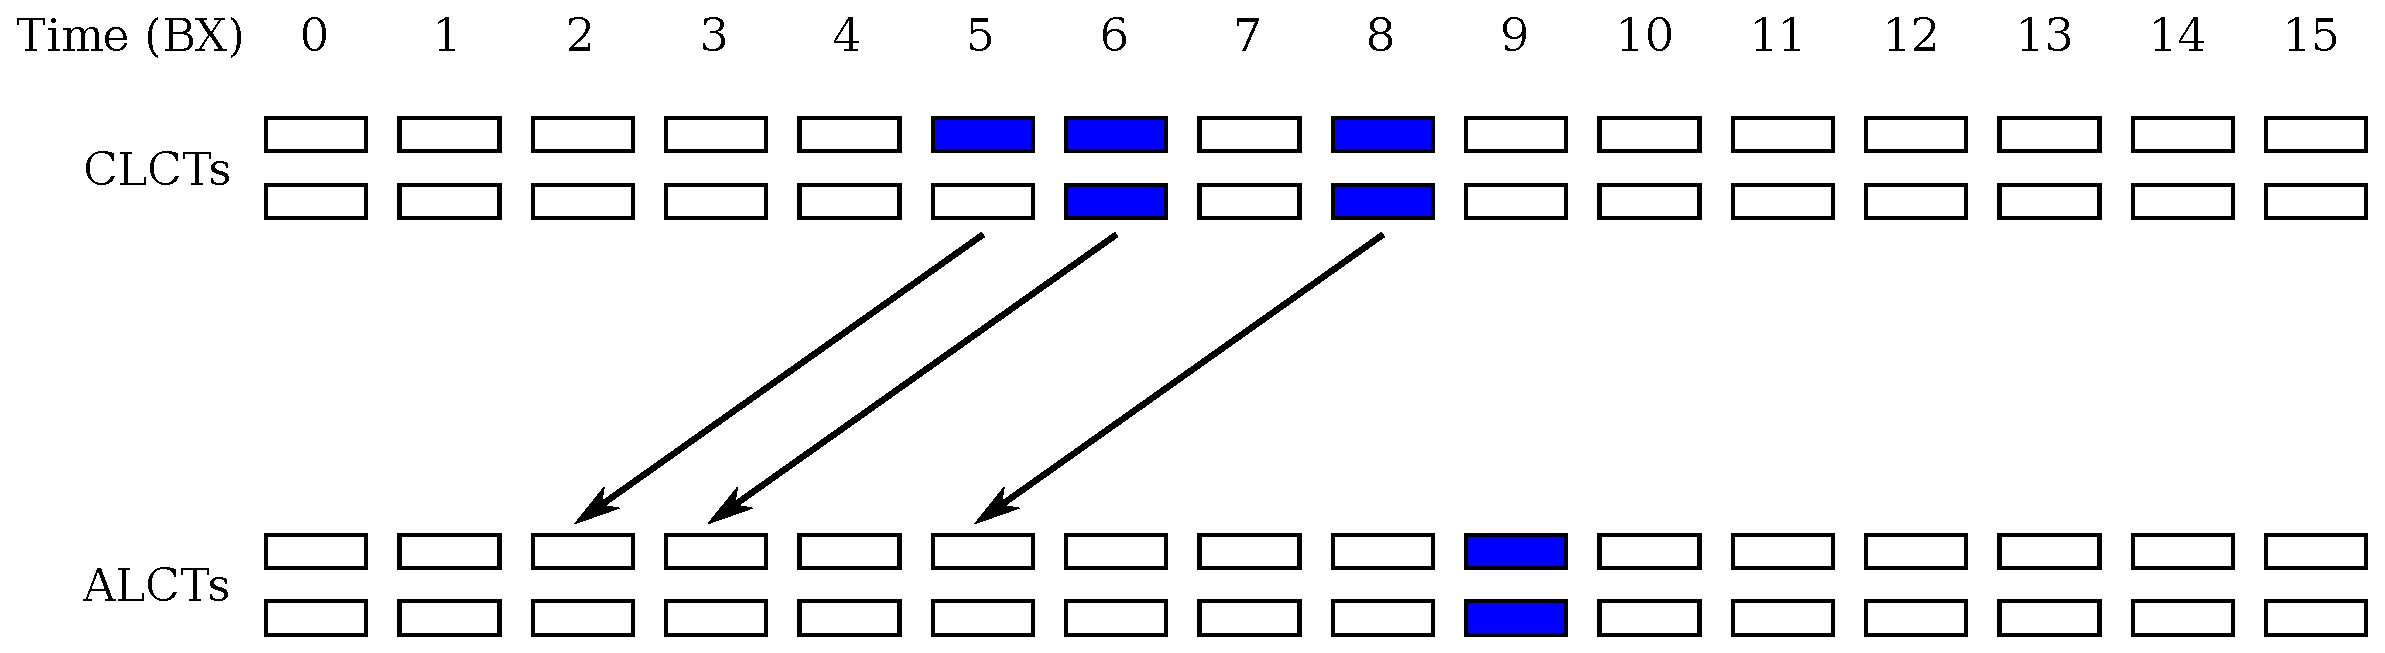
\includegraphics[width=0.7\linewidth]{figures/clct_alcts_alctless_end.pdf}
                \caption{Results of construction of ALCT-less LCTs.}
                \label{fig:clct_alcts_alctless_end}
        \end{center}
\end{figure}

If there are no valid CLCTs in the current CLCT BX and CLCT-less LCTs are allowed (see example on Fig.~\ref{fig:clct_alcts_clctless} with results on Fig.~\ref{fig:clct_alcts_clctless_end}):
\begin{itemize}
    \item Find first ALCT BX in the matching window with at least one valid ALCT and not marked as used before;
    \item Construct LCTs from valid ALCTs in that ALCT BX.
\end{itemize}

\begin{figure}[tbh]
        \begin{center}
                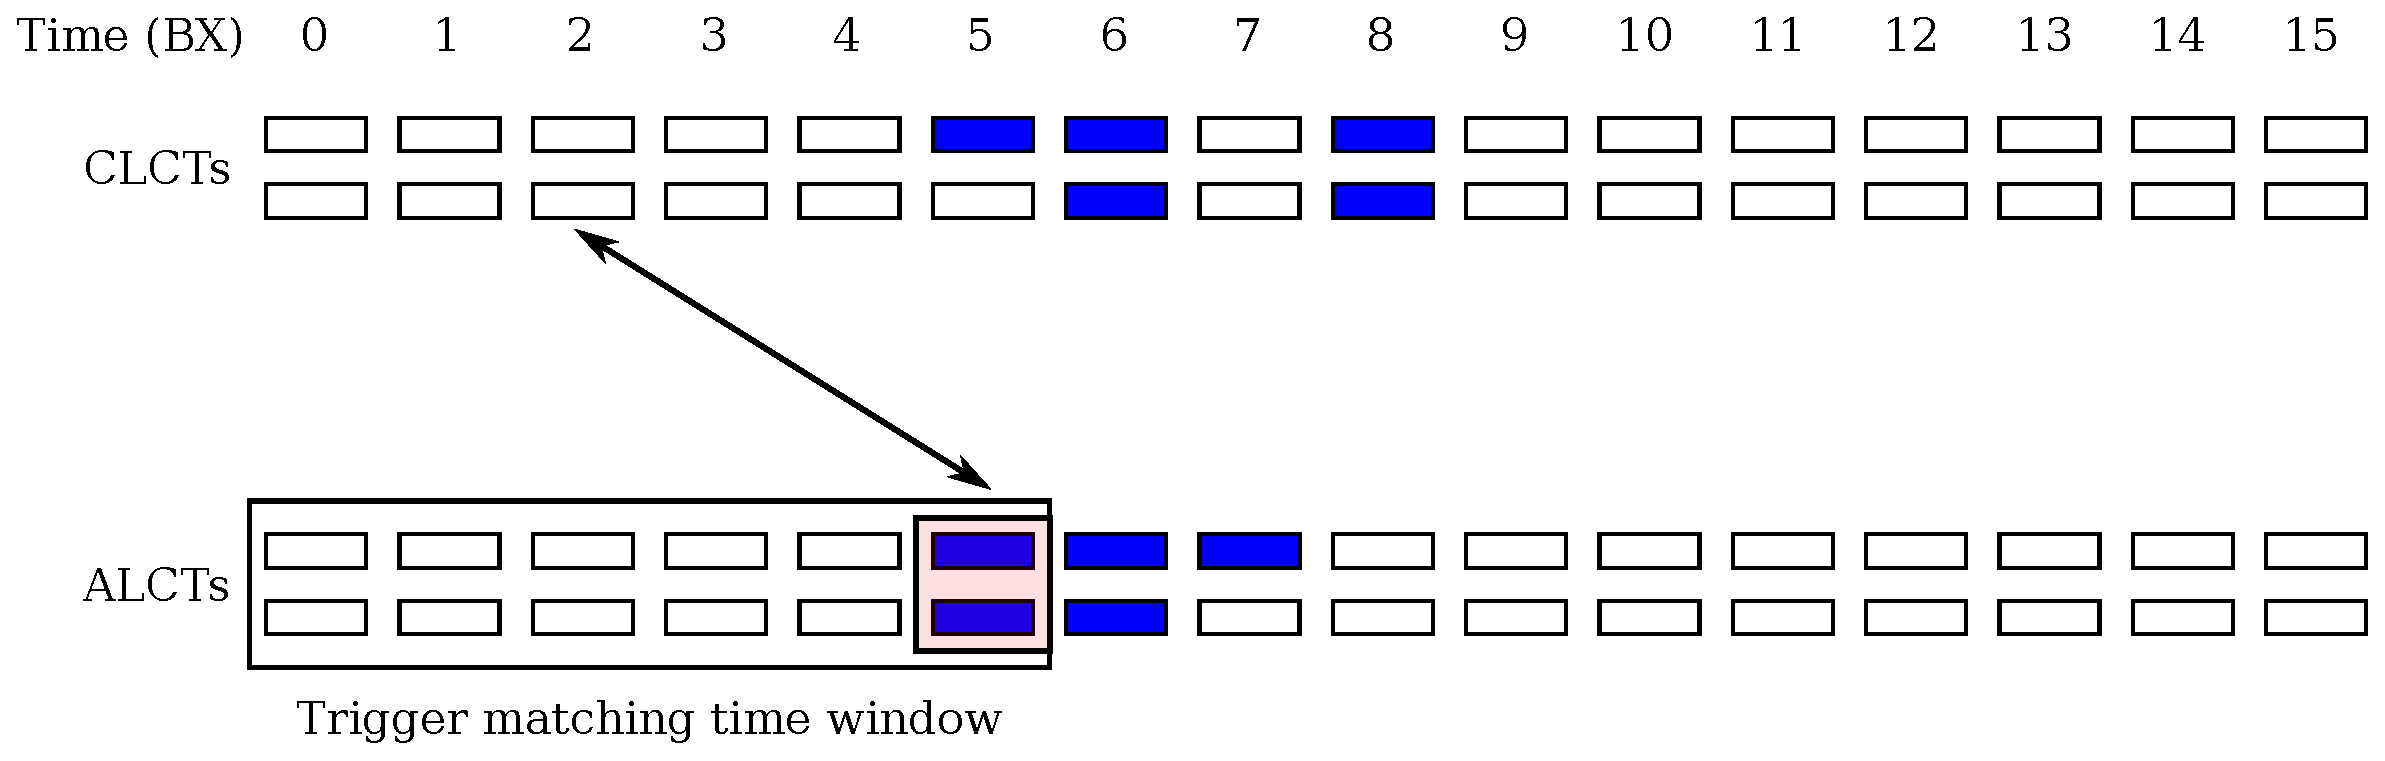
\includegraphics[width=0.7\linewidth]{figures/clct_alcts_clctless.pdf}
                \caption{Example of construction of CLCT-less LCTs.}
                \label{fig:clct_alcts_clctless}
        \end{center}
\end{figure}

\begin{figure}[tbh]
        \begin{center}
                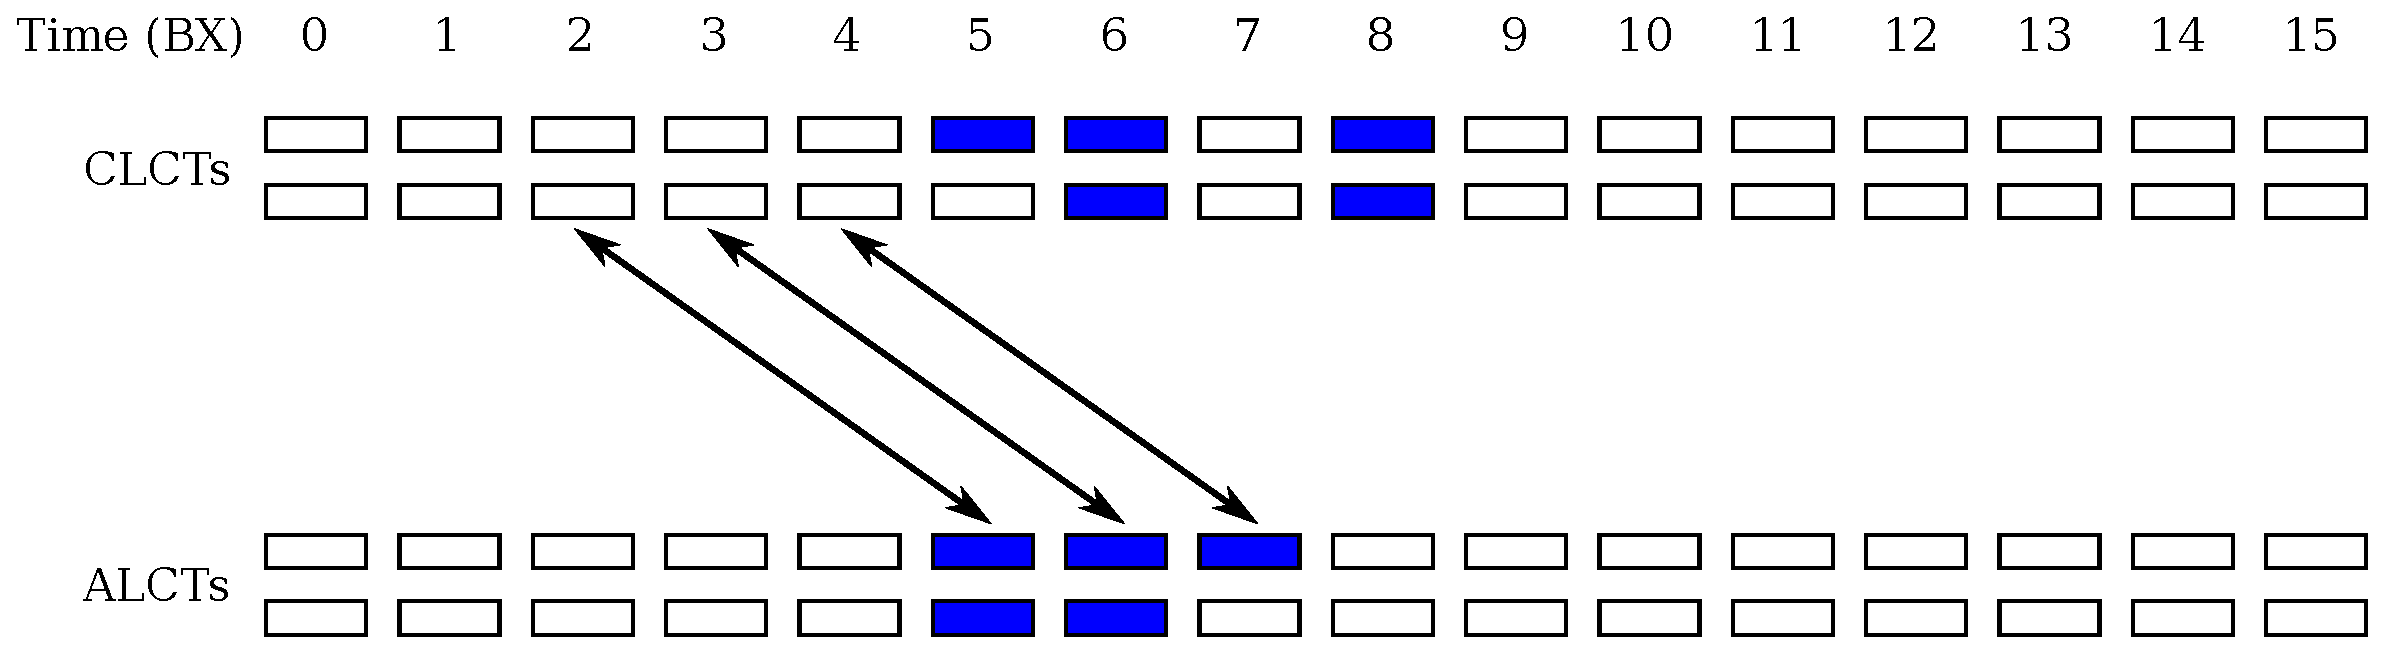
\includegraphics[width=0.7\linewidth]{figures/clct_alcts_clctless_end.pdf}
                \caption{Results of construction of CLCT-less LCTs.}
                \label{fig:clct_alcts_clctless_end}
        \end{center}
\end{figure}

When we use default behavior, where LCTs are constructed only from valid CLCTs and ALCTs, the ideal case is when in matching BXs number of valid CLCTs is equal to number of valid ALCTs (see top two examples on Fig.~\ref{fig:clct_alct_corr}).

\begin{figure}[tbh]
        \begin{center}
                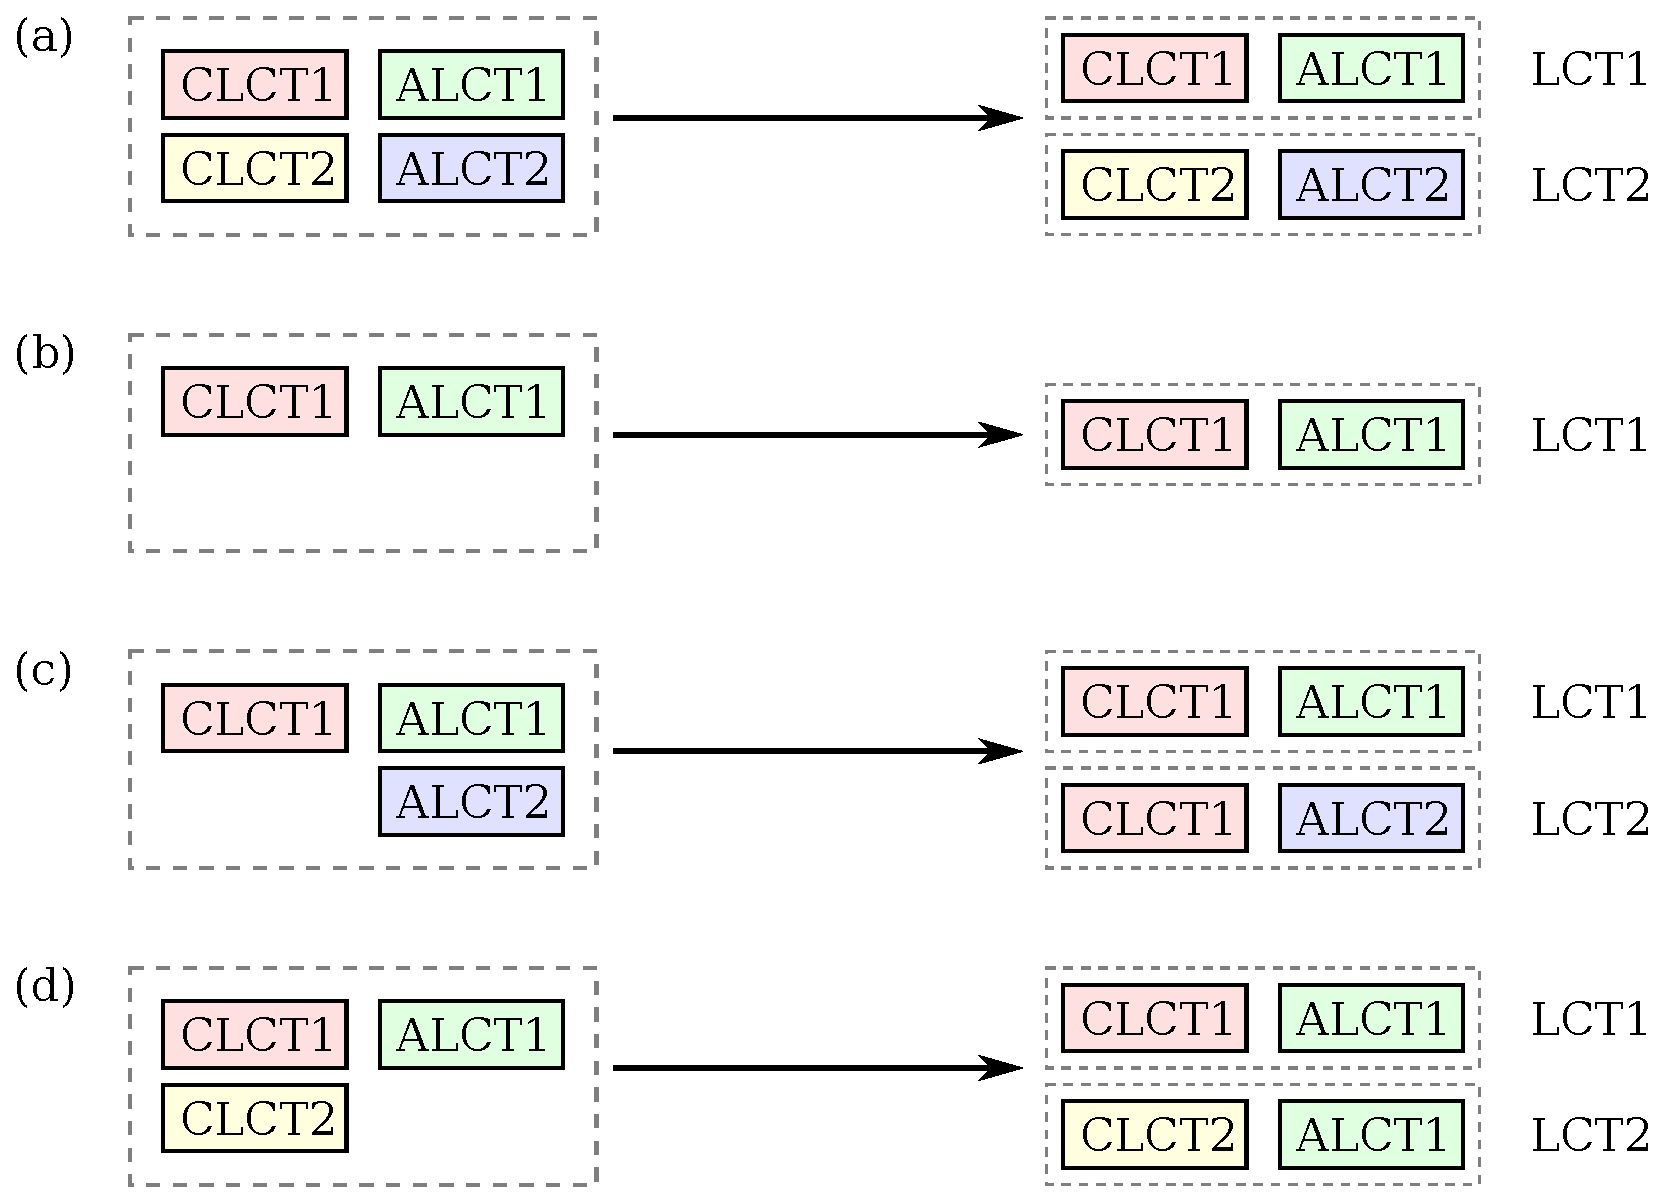
\includegraphics[width=0.7\linewidth]{figures/clct_alct_corr.pdf}
                \caption{Construction of LCTs.}
                \label{fig:clct_alct_corr}
        \end{center}
\end{figure}

But when, for example, there is only one valid CLCT and two valid ALCTs, we make the second valid CLCT from the first, analogously, when there are two valid CLCTs and only one valid ALCT (see bottom two examples on Fig.~\ref{fig:clct_alct_corr}).
\clearpage

\newpage
\tracinginput{sections/algorithm_SLHC.tex}
%\section{Improved CSC Trigger Algorithm for High Luminosity Running}
\label{sec:SLHC_algo}

\subsection{Separate finding of CLCTs in ME1/a and ME/1b}

 In the old TMB f/w, the 16 ganged strip channels from ME1/a are appended to the 64 ME/1b strip channels and the reconstruction of CLCTs is performend as if it's a single regular chamber with 80 channels (is there any treatment of the boundary, so that ME1/a strips are not combined with ME1/b strips?). The two rather separate and distinctive areas combined and treated like one uniform unit with the maximum of two CLCT stubs on the output.

With unganged ME1/a and higher pile-up such a simple approach becomes increaingly unnatural and ineffective. The ME1/a would have x3 more channels now, so it would deserve to be treated like a seperate chamber even more. And chances to get multiple stubs are increasing with higher luminosity, especially so in ME1/a. With multiple stubs, the stubs in ME1/a would start directly competing with those in ME1/b.

With a larger size FPGA, it would be beneficial to treat ME1/a and ME1/b as two separate chambers for the purpose of CLCT reconstruction, with each area having their own limit on the maximum of 2 CLCTs. Thus, the whole ME1/1 would be able to have maximum 4 CLCTs available for matching with ALCTs. It's important to keep more 2D stubs available so that at the stage of matching we can reduce the number of stubs following some better tuned criteria.

Finally, in the case if we would allow to read out the 2D CLCT stubs without an ALCT match, and we cannot read out more then 2 of them per BX per ME1/1, we can device a selection criteria when comparing stubs from ME1/a and 1/b as follows: e.g., if quality of an ME1b stub is the same or less by one then that of an MEr 1a stub, prefer the ME1b one. 

\subsection{Localizing the TMB dead time }

 The main source of the old TMB inefficiency in high pile-up is the dead time which happens for the whole ME1/1 chamber after there was a triggering CLCT. The TMB's state-machine freezes whole TMB for several BXs after a CLCT trigger while number of coincidence layers stays over the trigger threshold. If anywhere in a chamber there was an CLCT from PU a few BX earlier before a signal muon, it would be impossible to trigger on the signal.

While it's clear that with the comparator information which we recieve in TMB, it's not really possible to distinguish close in time signals in the same strip, there seem to be no apparent reason, other then the complexity of the algorithm, for this dead time to be present in strips that had no trigger.

Thus, the algorithm approach to deal with this issue for the upgrade could be as follows:
\begin{itemize}
    \item when a CLCT trigger happens, mark as busy only those strips within either a fixed dead time zone around CLCT (8 half-strips, see "useDeadTimeZoning" parameter in Sec.~\ref{sec:CLCT_conf}) or within the dead time zone, the width of which depends on the CLCT pattern (from 11 half-strips for the most bent patterns to 3 half-strips for the straightest one, see "useDynamicStateMachineZone" parameter in Sec.~\ref{sec:CLCT_conf}), and also mark the signal half-strip that specifies the triggered CLCT
    \item during the following bunch-crossings, check if the number of coincidence layers drops under the trigger threshold for the signal half-strip
    \begin{itemize}
	\item if it does, remove the "busy" mark from the corresponding strips 
    \end{itemize}
    \item if strips are marked as busy in a BX, they are excluded from pattern recognition 
\end{itemize}

\subsection{Restriction of CLCT pattern bend }

 The current set of CLCT patterns (e.g., see p5 of TMB2005\_spec\_v4p55) is largely geared towards low pt tracks. For tracks with pt>10, only the straighest and the next one bent patterns are significant. The restriction on allowed pattern bending would significantly help with many issues including multiplicity \& rate, ghosting, dead-time and corresponding loss of the efficiency (see "clctPidThreshPretrig" parameter in Sec.~\ref{sec:CLCT_conf}). Positive effect of it would increase with increasing luminosity. However, it would also somewhat reduce the efficiency because of not so good pt-threshold resolution from fairly narrow (11cm) CSC chambers, especially for medium to lower pt muons.

TODO: need a plot showing the efficiency vs pt for a simtrack to have a matching reconstricted CLCT stub for different maximum thresholds for the bend. GEMs could be helpful for improving the effectivenes and the efficiency of the bend restriction. 

\subsection{Improving CLCT timing }

 Currently, the BX time of a CLCT stub is defined as the BX of its pretrigger. Or, in other words, it's first BX when at least three layers fit one of the CLCT patterns. Note that an attempt to latch a trigger pattern is performed after the number of BX after the pretrigger defined by the clctDriftDelay parameter (=2BX). And also note that a CLCT pattern during the pretrigger could be different then the one that happen to match during the trigger.

With higher luminosity there are increasingly larger chances for some strips in some of the layers to be hit by earlier background hit. And that has chances to affect the time when a pretrigger might be detected. A more robust solution would be to define stub's time using the times of its strips, where stub's strips are defined as strips that were matched within a CLCT pattern during the trigger. As for a specific procedure, a median time over those strips' times or some sort of a truncated average could be used (see "clctUseCorrectedBx" parameter in Sec.~\ref{sec:CLCT_conf}, analogously for "alctUseCorrectedBx" parameter in Sec.~\ref{sec:ALCT_conf}).

\subsection{ALCT Handling }

 It should be possible to improve the efficiency, rate and timing precision of ALCT stubs by, e.g.
\begin{itemize}
    \item tuning of the ghost cancellation logic (ALCTs in neighboring wiregroups, see "alctGhostCancellationBxDepth" and "alctGhostCancellationSideQuality" parameters in Sec.~\ref{sec:ALCT_conf}) and removing pre-trigger deadtime (see "alctPretrigDeadtime" parameter in Sec.~\ref{sec:ALCT_conf});
    \item using more narrow ALCT pattern in ring 1 chambers (see "alctNarrowMaskForR1" parameter in Sec.~\ref{sec:ALCT_conf});
    \item using more precise algorithm (e.g., running median or truncated average) for BX assignment (see "alctUseCorrectedBx"  parameter in Sec.~\ref{sec:ALCT_conf}).
\end{itemize}

However, here we would only like to focus on how the ALCT stubs would be used by TMB.

ALCTs are reconstructed from the signals in layers of anode wires which are ganged into wiregroups and are continuously covering the whole ME1/1 chamber. Most of the wiregroups can only physically cross only strips either in ME1/a or only in ME1/b. A complication specific to ME1/1 is that wires here are not perpendicular to strips, but are slanted at 29 degrees from the straight angle. Thus, some wiregroups are crossing the border between ME1/a and ME1/b. If signal is detercted in such a wiregroup, there is an ambiguity about which part of ME1/1 it might belong to.

For the ALCTs received by TMB we propose to split the incoming stubs into two parts, ME1/a and ME1/b, that would be used further for LCT matching separately in ME1/a and ME1/b. 

\subsection{Narrowing the matching time window }

 The current TMB uses a rather wide time matching window (7BX) that is centered on a CLCT's BX, and is used to look for an ALCT match within it. A wide matching window is not good in high pileup, as propability of incorrect matching with background 2D stubs is higher, resulting in inefficiency.

For the SLHC, we can probably assume that the system is well timed and that we can use the narrowest reasonable matching window of 3BX wide (see "matchTrigWindowSize" parameter in Sec.~\ref{sec:TMB_conf}). 

\subsection{Modification of the stub timing logic in matching }

 In the old TMB algorithm, the stub timing logic works during the 2D stubs matching as follows:
\begin{itemize}
    \item CLCT-centric approach: CLCTs and their BX are taken as reference points, while ALCTs are waiting in a queue
    \item for a BX with CLCTs we look for a first BX in the matching window that has ALCTs
    \item after matching is dome in this BX, the ALCTs from there are taken off the queue, and cannot be matched with any later CLCT (see "tmbDropUsedClcts" and "matchEarliestClctME11Only" parameters in Sec.~\ref{sec:TMB_conf})
\end{itemize}

The main issues with this approach at high luminosity is that when there is an ALCT from a good signal muon, early CLCTs from background might steal it and form wrong match, and this correct ALCT then would not be available anymore for matching with a later correct CLCT.

Proposal to improve the situation:
\begin{itemize}
    \item ALCT-centric approach: ALCTs and their BXs are taken as reference points, while reconstructed CLCTs are waiting in a matching window-wide queue (see "clctToAlct" parameter in Sec.~\ref{sec:TMB_conf})
    \begin{itemize}
        \item ALCT's BX and the middle BX in the matching window-wide queue are expected to be synchronized 
    \end{itemize}
    \item for an ALCT's BX we look for CLCTs within the queue in the order of arrival try to find maximum 2 LCT matches as follows (see "tmbCrossBxAlgorithm" parameter in Sec.~\ref{sec:TMB_conf}):
    \begin{itemize}
        \item first look for CLCTs in the same BX 2) if we didn't get 2 LCT matches yet, look for CLCTs in BX-1
        \item if we didn't get 2 LCT matches yet, look for CLCTs in BX+1
        \item etc... depending on how wide the matching window is 
    \end{itemize}
    \item can optionally either remove CLCTs from the queue after there was an LCT match, or can keep them for reuse possibilities to be matched with later ALCTs (see "tmbDropUsedClcts" parameter in Sec.~\ref{sec:TMB_conf})
    \item NOTE: all this is supposed to be done separately in ME1a and in ME1b 
\end{itemize}

\subsection{Selecting up to two the best LCTs per ME1/1}

With the backplane limitations, we can read out only up to two trigger stubs per BX from the whole ME1/1.

Since ME1/a and ME1/b now can each have up to two stubs, we need an extra step of selecting the best two ME1/1 stubs out of possible 4. If ME1/a + ME1/b has more then two LCTs:
\begin{itemize}
    \item The simplest solution:
    \begin{itemize}
	\item drop the highest eta ones until we have just two. 
    \end{itemize}
    \item Possible improvement:
    \begin{itemize}
        \item rank stubs by special quality value which is the same as stub quality for ME1/b and is stub quality-1 for ME1/a stubs
        \item if special quality is the same, rank by eta 
    \end{itemize}
\end{itemize}

\newpage
\subsection{Sofware Emulation of ALCT Level Improvements}

\subsubsection{Tuning of Ghost Cancellation Procedure}

\textcolor{red}{Current} ghost cancellation:
\begin{itemize}
    \item Loop over wire groups:
    \begin{itemize}
        \item Consider WG = N
        \item Cancel trigger in this wire group if there is trigger in WG = N-1 and:
        \begin{itemize}
            \item with the same BX and with \textcolor{red}{better or equal} quality
            \item up to \textcolor{red}{4} BXs earlier, with \textcolor{red}{any} quality
        \end{itemize}
        \item Cancel trigger in this wire group if there is trigger in WG = N+1 and:
        \begin{itemize}
            \item with the same BX and with \textcolor{red}{better} quality
            \item up to \textcolor{red}{4} BXs earlier, with \textcolor{red}{any} quality
        \end{itemize}
    \end{itemize}
\end{itemize}
\textcolor{blue}{New} ghost cancellation:
\begin{itemize}
    \item Loop over wire groups:
    \begin{itemize}
        \item Consider WG = N
        \item Cancel trigger in this wire group if there is trigger in WG = N-1 and:
        \begin{itemize}
            \item with the same BX and with \textcolor{blue}{better} quality
            \item up to \textcolor{blue}{1} BX earlier, with \textcolor{blue}{better} quality
        \end{itemize}
        \item Cancel trigger in this wire group if there is trigger in WG = N+1 and:
        \begin{itemize}
            \item with the same BX and with \textcolor{blue}{better or equal} quality
            \item up to \textcolor{blue}{1} BX earlier, with \textcolor{blue}{better and equal} quality
        \end{itemize}
    \end{itemize}
\end{itemize}

The following modifications in configuration are related to this improvement:
\begin{itemize}
    \item alctGhostCancellationBxDepth: 4BX to 1BX
    \item alctGhostCancellationSideQuality: False to True
\end{itemize}

\subsubsection{Narrow ALCT Pattern Mask}

Use more narrow ALCT pattern mask for stations in Ring 1 (see Fig.~\ref{fig:narrow_alct_pattern_mask}).

\begin{figure}[tbh]
        \begin{center}
                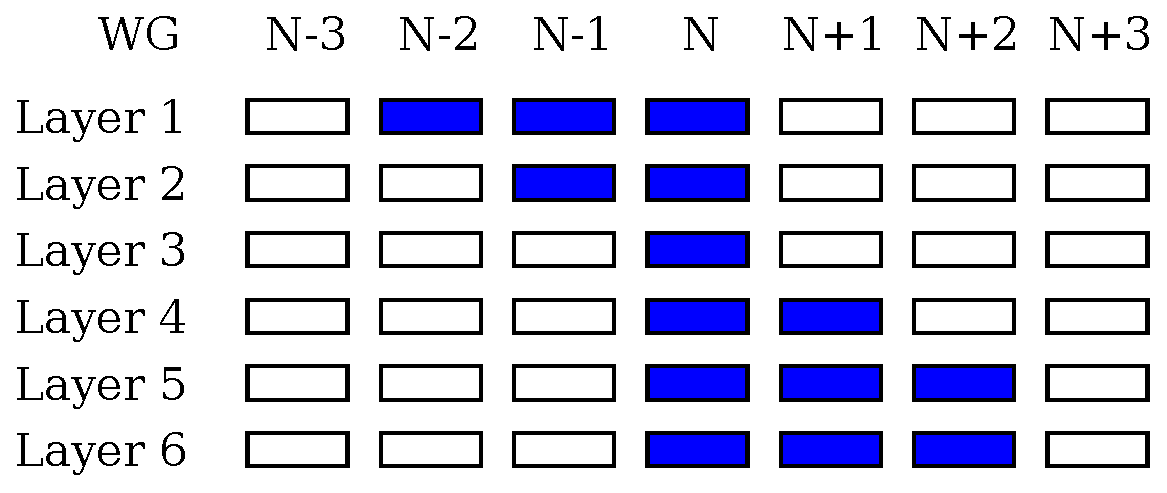
\includegraphics[width=0.49\linewidth]{figures/alct_pretrigger.pdf}\\
                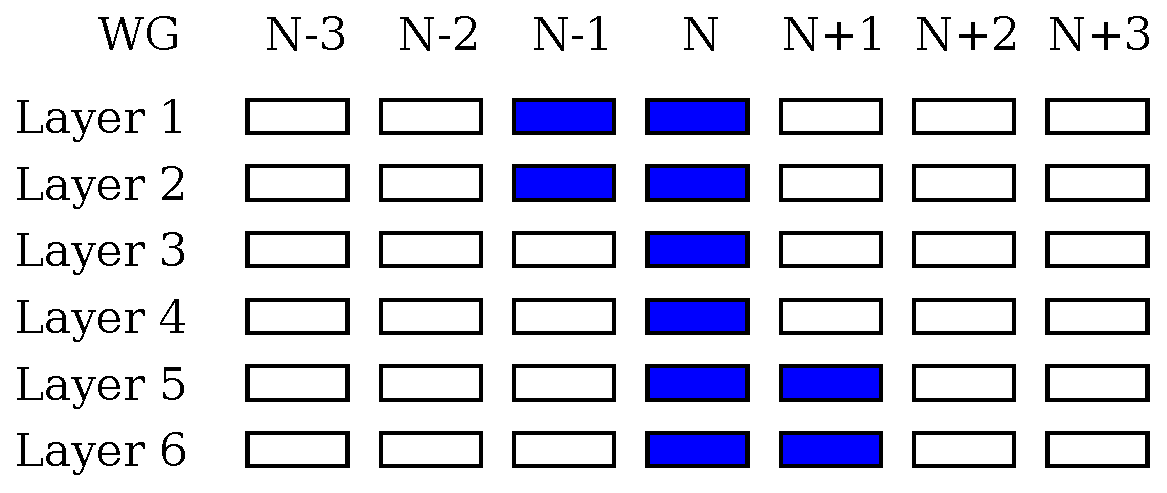
\includegraphics[width=0.49\linewidth]{figures/alct_pretrigger_r1.pdf}
                \caption{Top: default ALCT pattern mask, bottom: narrow ALCT pattern mask.}
                \label{fig:narrow_alct_pattern_mask}
        \end{center}
\end{figure}

The following modifications in configuration are related to this improvement:
\begin{itemize}
    \item alctNarrowMaskForR1: False to True
\end{itemize}

\subsubsection{Reduced ALCT Dead Time}

Currently, if there is pretrigger in BX = B (see Fig.~\ref{fig:alct_deadtime}):
\begin{itemize}
    \item Check for trigger in BX = B + drift time = B+2
    \item Search for next pretrigger starting from BX = B + drift time + extra deadtime = B+6
\end{itemize}

Suggested improvement: decrease extra deadtime from 4 BX to 0 BX.

\begin{figure}[tbh]
        \begin{center}
                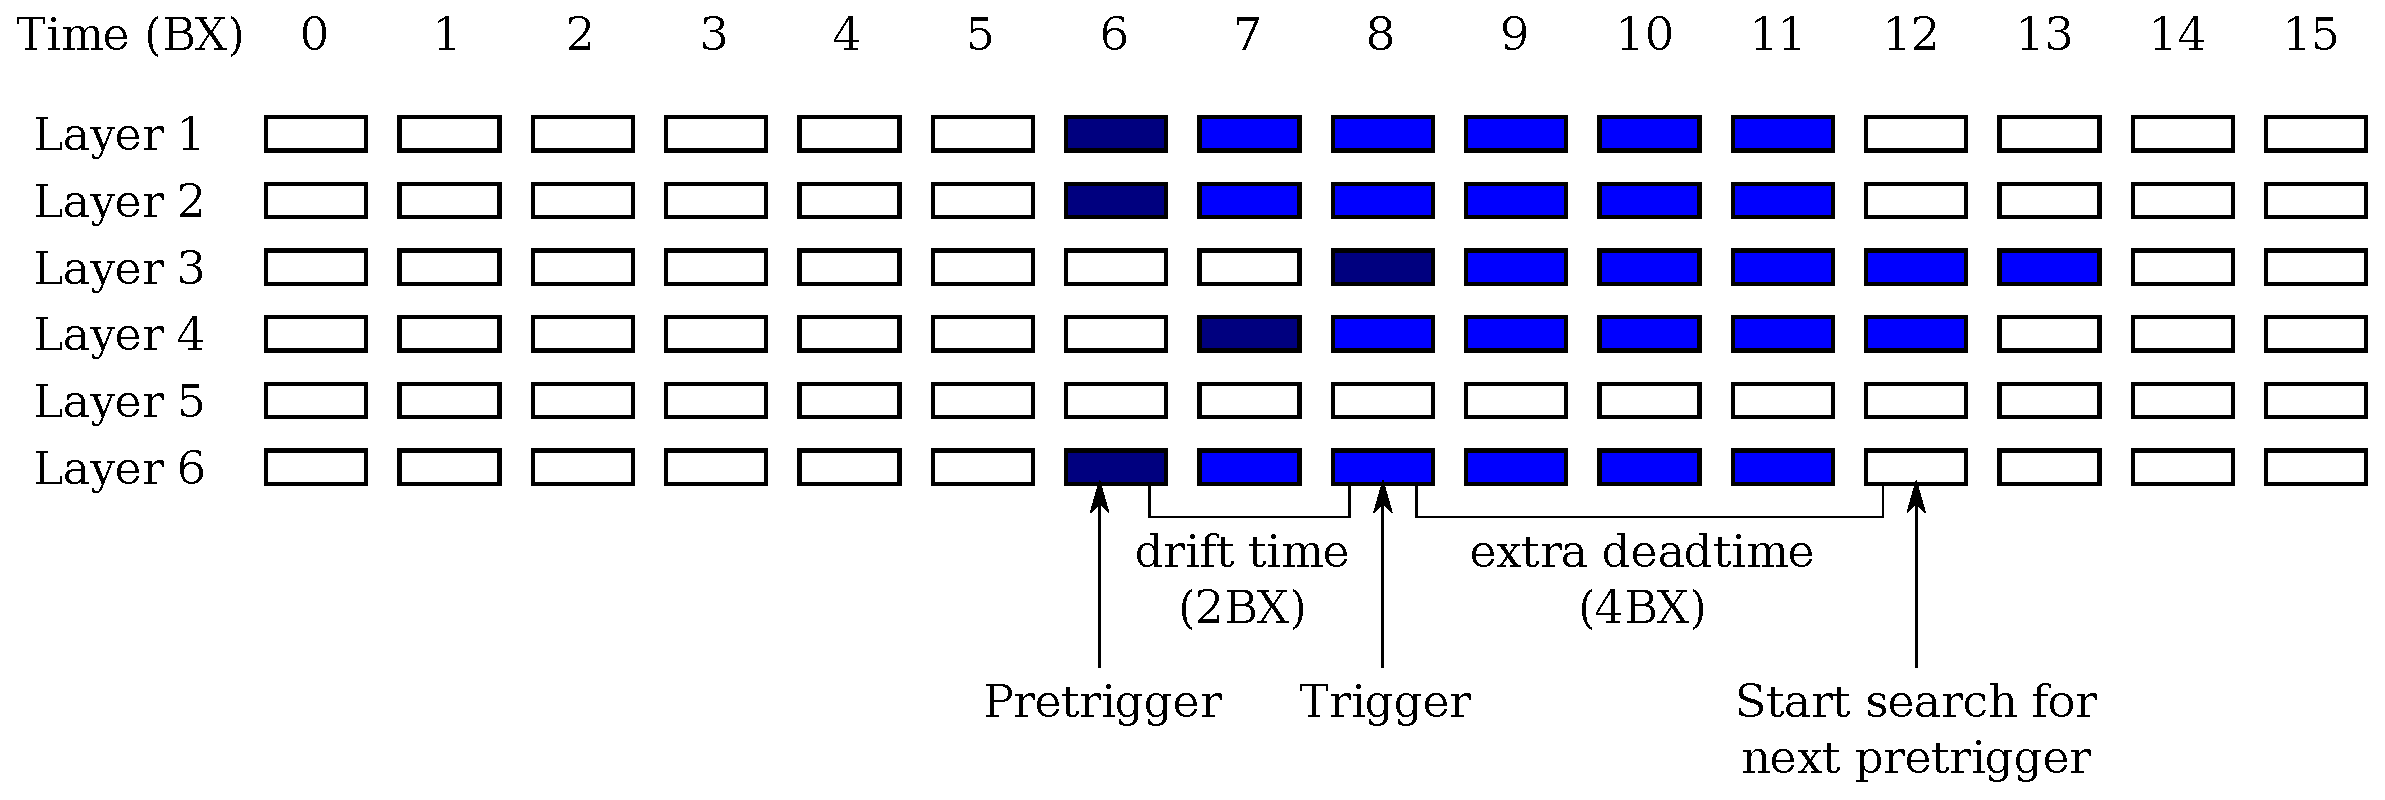
\includegraphics[width=0.98\linewidth]{figures/stretched_hits_alct_deadtime.pdf}
                \caption{Top: Dead Time between ALCT pretriggers.}
                \label{fig:alct_deadtime}
        \end{center}
\end{figure}

The following modifications in configuration are related to this improvement:
\begin{itemize}
    \item alctPretrigDeadtime: 4BX to 0BX
\end{itemize}

\newpage
\subsection{Sofware Emulation of CLCT Level Improvements}

\subsubsection{Localizing Dead Zone}

\textcolor{red}{Current implementation of dead time}:
\begin{itemize}
    \item After constructing up to two CLCTs, \textcolor{red}{continue the loop over all BXs until there is a BX with no triggers}
    \\...
    \item In the BX with trigger, construct up to two CLCTs from two best triggers \textcolor{red}{in all half-strips}
    
\end{itemize}
\textcolor{blue}{New implementation of dead time}:
\begin{itemize}
    \item After constructing up to two CLCTs, \textcolor{blue}{mark 16 half-strips around half-strips of these CLCTs as busy while number of hit layers in half-strips of these CLCTs $\geq$ 4}
    \item \textcolor{blue}{After trigger in BX = B, keep searching for pretrigger in strating from BX = B+1}
    \\...
    \item In the BX with trigger, construct up to two CLCTs from two best triggers \textcolor{blue}{in half-strips}
    \begin{itemize}
        \item \textcolor{blue}{within 5 half-strips from pretrigger half-strips}
        \item \textcolor{blue}{which are not marked as busy from previous trigger}
    \end{itemize}
\end{itemize}

The following modifications in configuration are related to this improvement:
\begin{itemize}
    \item useDeadTimeZoning: False to True
\end{itemize}

\subsubsection{Dynamic Dead Zone Width}

\textcolor{red}{Fixed dead time zone}:
\begin{itemize}
    \item After constructing up to two CLCTs, mark \textcolor{red}{16} half-strips around half-strips of these CLCTs as busy while number of hit layers in half-strips of these CLCTs $\geq$ 4
\end{itemize}
\textcolor{blue}{Dynamic dead time zone}:
\begin{itemize}
    \item After constructing up to two CLCTs, mark \textcolor{blue}{K(pid)} half-strips around half-strips of these CLCTs as busy while number of hit layers in half-strips of these CLCTs $\geq$ 4
\end{itemize}
\vskip3mm
K(pid) --- function of pattern id:
\begin{itemize}
    \item K(1,2,3) = 22 half-strips
    \item K(4,5) = 18 half-strips
    \item K(6,7) = 14 half-strips
    \item K(8,9) = 10 half-strips
    \item K(10) = 6 halt-strips
\end{itemize}

The following modifications in configuration are related to this improvement:
\begin{itemize}
    \item useDynamicStateMachineZone: False to True
\end{itemize}

\newpage

\subsubsection{Minimal Pattern ID for Pretriggering}

\textcolor{red}{Current CLCT pretrigger}:
\begin{itemize}
    \item Loop over all BXs (starting from BX = 0) and all half-strips:
    \begin{itemize}
        \item Count number of layers with hits in the following patterns
        \item If this number $\geq$ 3: pretrigger occurs
        \item Accept this pretrigger if its pattern id $\geq$ \textcolor{red}{2}
    \end{itemize}
\end{itemize}
\textcolor{blue}{New CLCT pretrigger}:
\begin{itemize}
    \item Loop over all BXs (starting from BX = 0) and all half-strips:
    \begin{itemize}
        \item Count number of layers with hits in the following patterns
        \item If this number $\geq$ 3: pretrigger occurs
        \item Accept this pretrigger if its pattern id $\geq$ \textcolor{blue}{4}
    \end{itemize}
\end{itemize}

The following modifications in configuration are related to this improvement:
\begin{itemize}
    \item clctPidThreshPretrig: 2 to 4
\end{itemize}

\subsubsection{Minimal Separation Between Two Best CLCTs}

\textcolor{red}{Current construction of up to two CLCTs}:
\begin{itemize}
    \item Search for the best trigger in this BX
    \item Mark \textcolor{red}{20} half-strips around the best trigger as busy
    \item Find the second best trigger among non-busy half-strips
\end{itemize}
\textcolor{blue}{New construction of up to two CLCTs}:
\begin{itemize}
    \item Search for the best trigger in this BX
    \item Mark \textcolor{blue}{10} half-strips around the best trigger as busy
    \item Find the second best trigger among non-busy half-strips
\end{itemize}

The following modifications in configuration are related to this improvement:
\begin{itemize}
    \item clctMinSeparation: 10 to 5 cathode strips
\end{itemize}

\newpage
\subsection{Sofware Emulation of TMB Level Improvements}

\subsubsection{Decreased Trigger Matching Window}

Decrease size of trigger matching time window from 7 BXs to 3 BXs (see Fig.~\ref{fig:clct_alcts_short_window}).

\begin{figure}[tbh]
        \begin{center}
                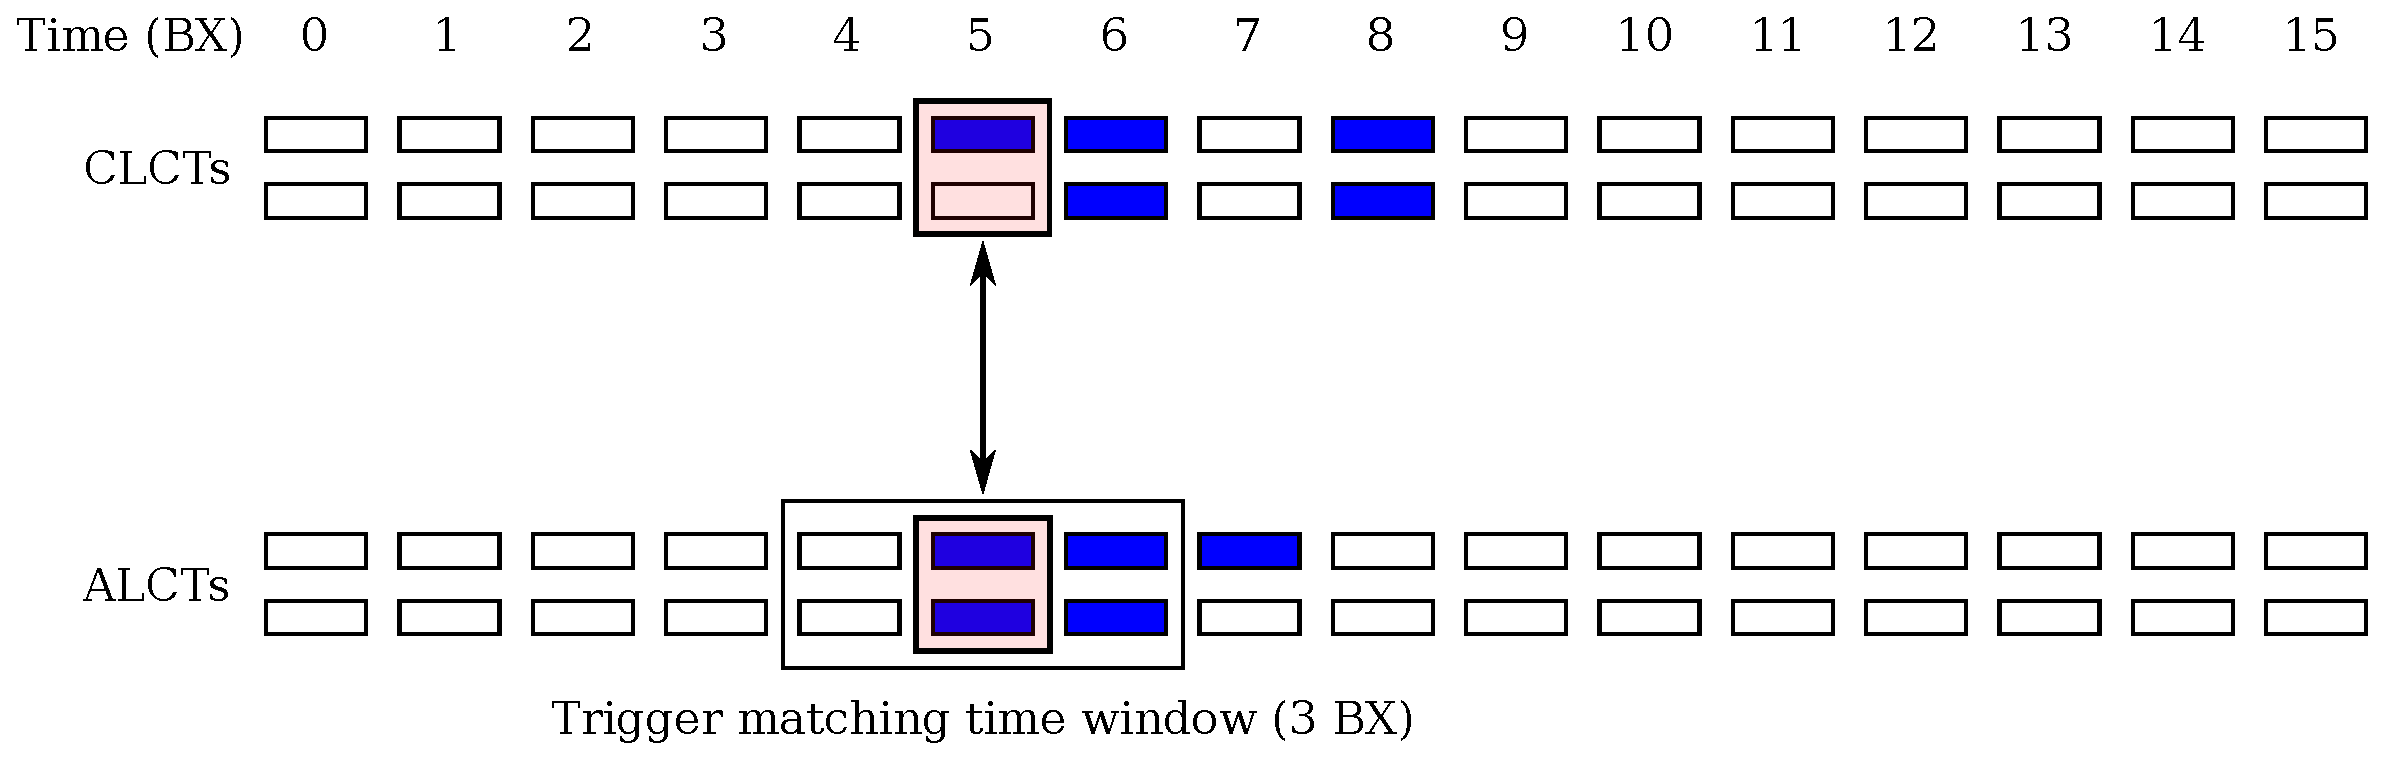
\includegraphics[width=0.98\linewidth]{figures/clct_alcts_short_window.pdf}
                \caption{Decreased trigger matching window.}
                \label{fig:clct_alcts_short_window}
        \end{center}
\end{figure}

The following modifications in configuration are related to this improvement:
\begin{itemize}
    \item matchTrigWindowSize: 7BX to 3BX
\end{itemize}

\subsubsection{ALCT-centric ALCT and CLCT Correlation}

Switch from CLCT-centric matching to ALCT-centric matching (see Fig.~\ref{fig:alct_clcts}).

\textcolor{red}{CLCT-centric matching}
\begin{itemize}
    \item Loop over CLCT BXs from BX = 0 to BX = 15
    \item For CLCT BX = B with at least one valid CLCT:
    \begin{itemize}
        \item Loop over ALCT BXs from BX = B-3 to BX = B+3
    \end{itemize}
\end{itemize}
\textcolor{blue}{ALCT-centric matching}
\begin{itemize}
    \item Loop over ALCT BXs from BX = 0 to BX = 15
    \item For ALCT BX = B with at least one valid ALCT:
    \begin{itemize}
        \item Loop over CLCT BXs from BX = B-3 to BX = B+3
    \end{itemize}
\end{itemize}

\begin{figure}[tbh]
        \begin{center}
                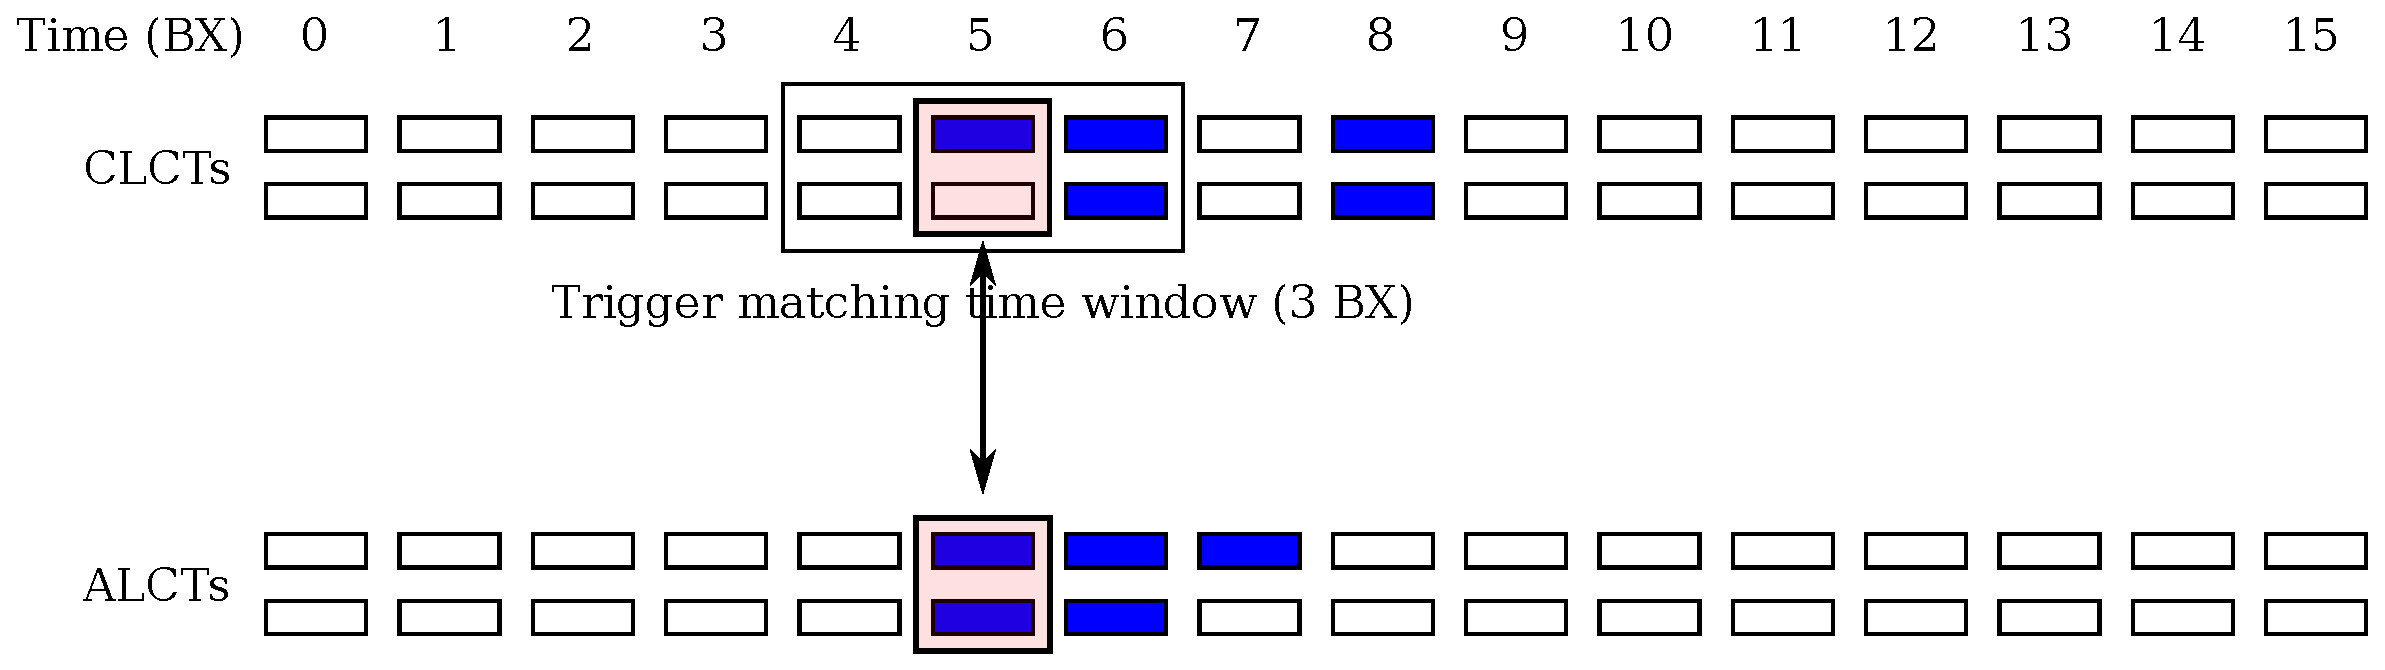
\includegraphics[width=0.98\linewidth]{figures/alct_clcts.pdf}
                \caption{ALCT-centric ALCT anc CLCT correlation.}
                \label{fig:alct_clcts}
        \end{center}
\end{figure}

The following modifications in configuration are related to this improvement:
\begin{itemize}
    \item clctToAlct: True to False
\end{itemize}

\subsubsection{Reusage of Used ALCTs and CLCTs}

Allow reusage of ALCTs and CLCTs already used during ALCT and CLCT correlation (see Fig.~\ref{fig:reuse_alct_clct}).

\textcolor{red}{Current behavior}:
\begin{itemize}
    \item Drop used CLCTs: do not use them with ALCTs in other ALCT BXs;
    \item Proceed to next ALCT BX after matching ALCTs with earliest CLCT BX with at least one valid CLCT.
\end{itemize}
\textcolor{blue}{New behavior}:
\begin{itemize}
    \item Do not drop used CLCTs: reuse them with ALCTs in other ALCT BXs;
    \item Match ALCTs to CLCTs in all CLCT BXs within matching window.
\end{itemize}

\begin{figure}[tbh]
        \begin{center}
                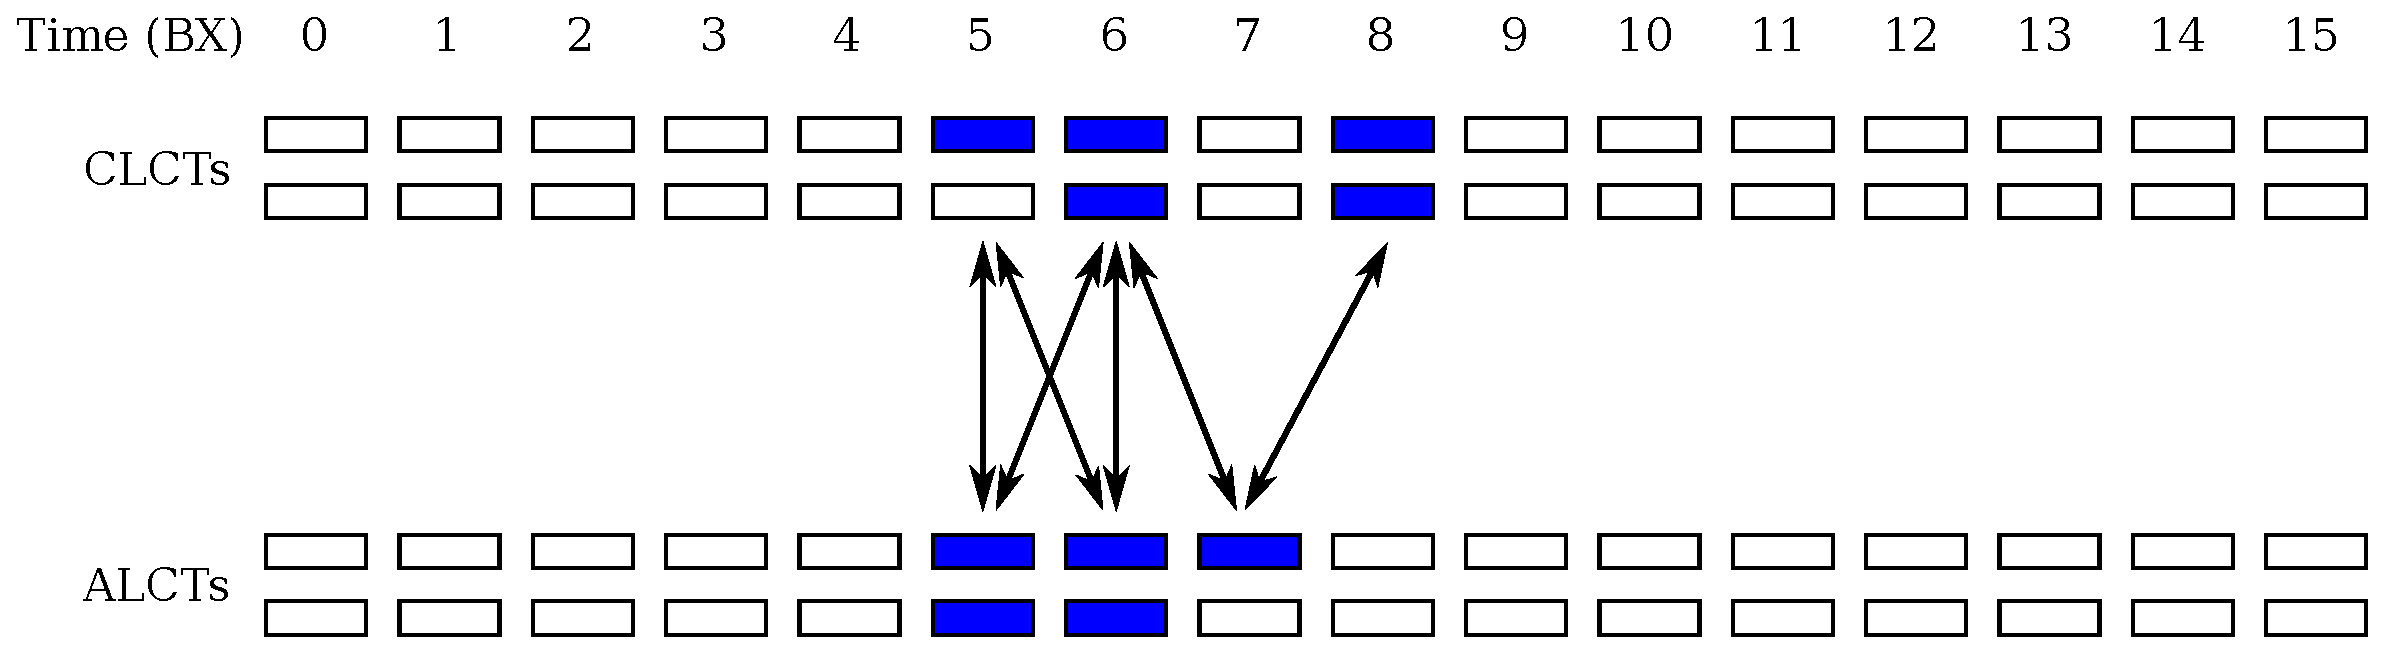
\includegraphics[width=0.98\linewidth]{figures/clct_alcts_end_2.pdf}
                \caption{Reusage of already used ALCTs and CLCTs.}
                \label{fig:reuse_alct_clct}
        \end{center}
\end{figure}

The following modifications in configuration are related to this improvement:
\begin{itemize}
    \item tmbDropUsedClcts: True to False
    \item matchEarliestClctME11Only: True to False
\end{itemize}

\subsubsection{Cross BX Algorithm}

In the situation shown on Fig.~\ref{fig:reuse_alct_clct}, in some given BX = B we can end up having with up to 6 LCTs (made from ALCTs in BX = B and CLCTs in BX = B-1, B, B+2. How do we choose two LCTs to be reported for BX = B?

\textcolor{red}{Current behavior: "cross bx" algorithm is turned off}
\begin{itemize}
    \item Choose two best LCTs with the highest quality
\end{itemize}
\textcolor{blue}{New behavior: "cross bx algorithm"}
\begin{itemize}
    \item Take LCTs with ALCT BX = B and CLCT BX = B
    \item If we still don't have two LCTs, take best ones with ALCT BX = B-1
    \item If we still don't have two LCTs, take best ones with ALCT BX = B+1
\end{itemize}

The following modifications in configuration are related to this improvement:
\begin{itemize}
    \item tmbCrossBxAlgorithm: 0 to 1
\end{itemize}

\newpage

\subsubsection{Corrected ALCT and CLCT Timing}

Use more robust procedure for assignment of ALCT BX and CLCT BX.

\textcolor{red}{Current behavior}:
\begin{itemize}
    \item Use ALCT and CLCT pretrigger BXs to assign ALCT BX and CLCT BX.
\end{itemize}
\textcolor{blue}{New behavior}:
\begin{itemize}
    \item For each hit in ALCT and CLCT trigger patterns, determine "first BX": BX of original hit before hit stretching over 6 BXs;
    \item For ALCTs, consider hits in key WG = N and two neighbouring WGs: WG = N-1 and WG = N+1;
    \item For CLCTs, consider all hits in the pattern;
    \item Store "first BXs" of these hits in two sorted sets (one for ALCT times and another for CLCT times);
    \item Use median elements in these sets to assign ALCT BX and CLCT BX.
\end{itemize}

The following modifications in configuration are related to this improvement:
\begin{itemize}
    \item alctUseCorrectedBx: False to True
    \item clctUseCorrectedBx: False to True
\end{itemize}

\subsubsection{Reading out more LCTs}

[I'm not sure I completely understand the meaning of this improvement]

\textcolor{red}{Current behavior}
\begin{itemize}
    \item In digi$\rightarrow$raw step, LCTs have to be packed into the TMB header, and currently there is room just for two
    \item Take LCTs only from earliest BX in L1A readout with at least one LCT
\end{itemize}
\textcolor{blue}{New behavior}
\begin{itemize}
    \item Take LCTs from the whole L1A readout (from BX = 5 to BX = 11)
\end{itemize}

The following modifications in configuration are related to this improvement:
\begin{itemize}
    \item tmbReadoutEarliest2: True to False
\end{itemize}

\newpage


\clearpage

\newpage
\tracinginput{sections/algorithm_SLHC_results.tex}
%\section{Study of Individual Improvements in the CSC Trigger Algorithm}
\label{sec:SLHC_algo_results}

This chapter presents results of the study of effects of individual improvements described in Sec.~\ref{sec:SLHC_algo} on the ALCT, CLCT, and LCT reconstruction efficiencies.

The study is performed with Monte Carlo simulation of double muon events mixed with PU400 events, where the simulation includes GEN, SIM, DIGI, L1 steps.

Three are three baseline configurations of L1 step used in this study:
\begin{itemize}
	\item Baseline 1: SLHC configuration, where the maximum set of improvements is turned off bringing it to 2007 configuration as close as possible. 
	There are only two differences between Baseline 1 and 2007 configurations: separate treatments of ME1a and ME1b, and unganging cathode strips in ME1a;
	\item Baseline 2: Baseline 1 configuration with all improvements on the ALCT and CLCT processors level turned on;
	\item SLHC configuration itself.
\end{itemize}

All algorithm improvements devided into three groups and studied with improvements in the given group turned on one by one on top of each other
\begin{itemize}
	\item ALCT processor level
	\item CLCT processor level
	\item TMB level
\end{itemize}

In the first two groups the L1 step configuration gradually changes from Baseline 1 to Baseline 2 configuration, in the last one --- from Baseline 2 to SLHC configuration.

\newpage

\subsection{ALCT Processor Level Improvements}

\begin{figure}[htb]
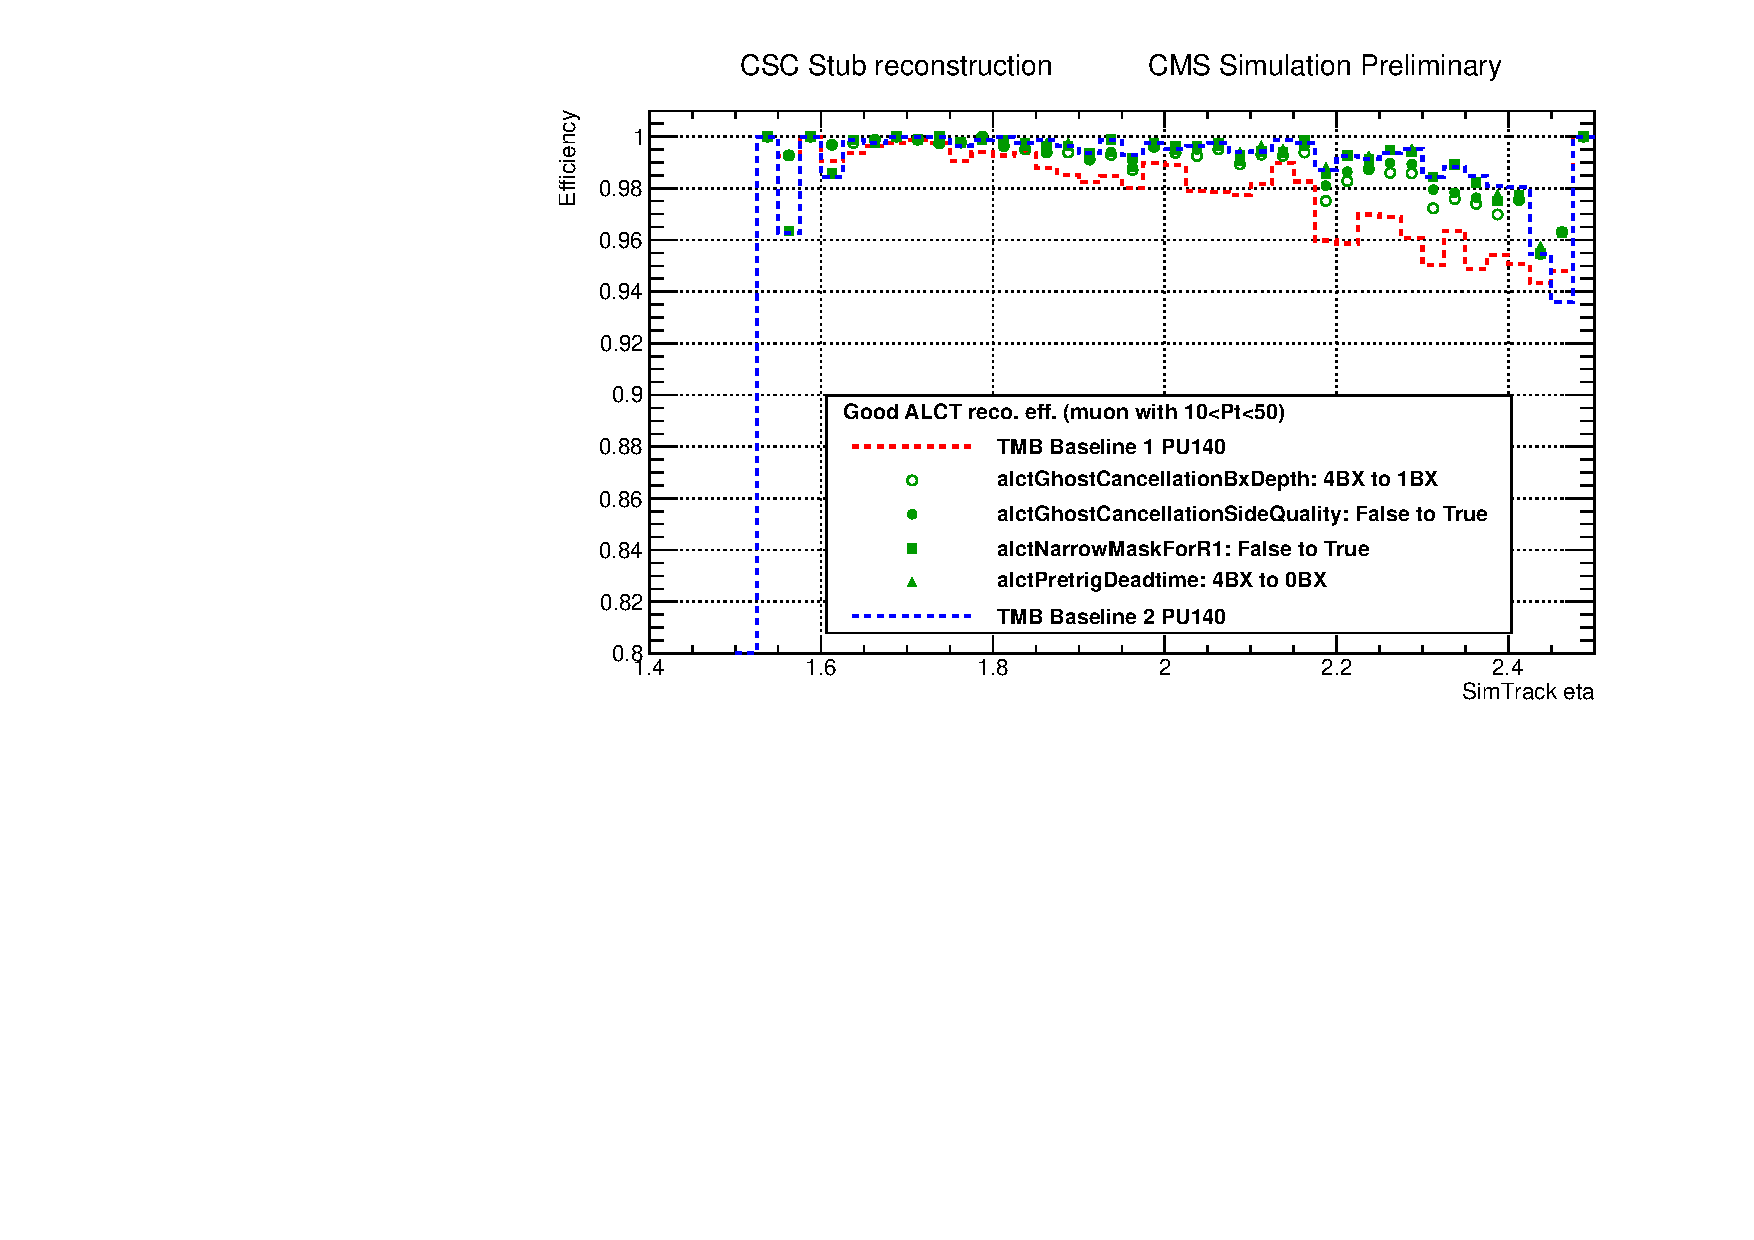
\includegraphics[width=0.98\textwidth]{figures/ALCT_improvements_ALCT_recoEff.pdf}
\caption{Reconstruction efficiency of a good ALCT in ME1 station}
\label{fig:ALCT_improvements_ALCT_recoEff}
\end{figure}

Improvements on the level of ALCT processor are related to the following configuration parameters (see Sec.~\ref{sec:ALCT_conf}):
\begin{itemize}
	\item alctGhostCancellationBxDepth: 4BX to 1BX;
	\item alctGhostCancellationSideQuality: False to True;
	\item alctNarrowMaskForR1: False to True;
	\item alctPretrigDeadtime: 4BX to 0BX.
\end{itemize}

Fig.~\ref{fig:ALCT_improvements_ALCT_recoEff} shows reconstruction efficiency of a good ALCT in ME1 station versus pseudorapidity of the simulated muon for different L1 configurations. The good ALCT is defined as ALCT:
\begin{itemize}
	\item read out in the window of 3BX around the central BX (BX6);
	\item reconstructed within 2 anode wire groups from the key wire group.
	\item has hits at least on three layers
\end{itemize}

The major improvement in ALCT reconstruction efficiency comes from the changes in ALCT ghost cancellation procedure.

\newpage

\subsection{CLCT Processor Level Improvements}

\begin{figure}[htb]
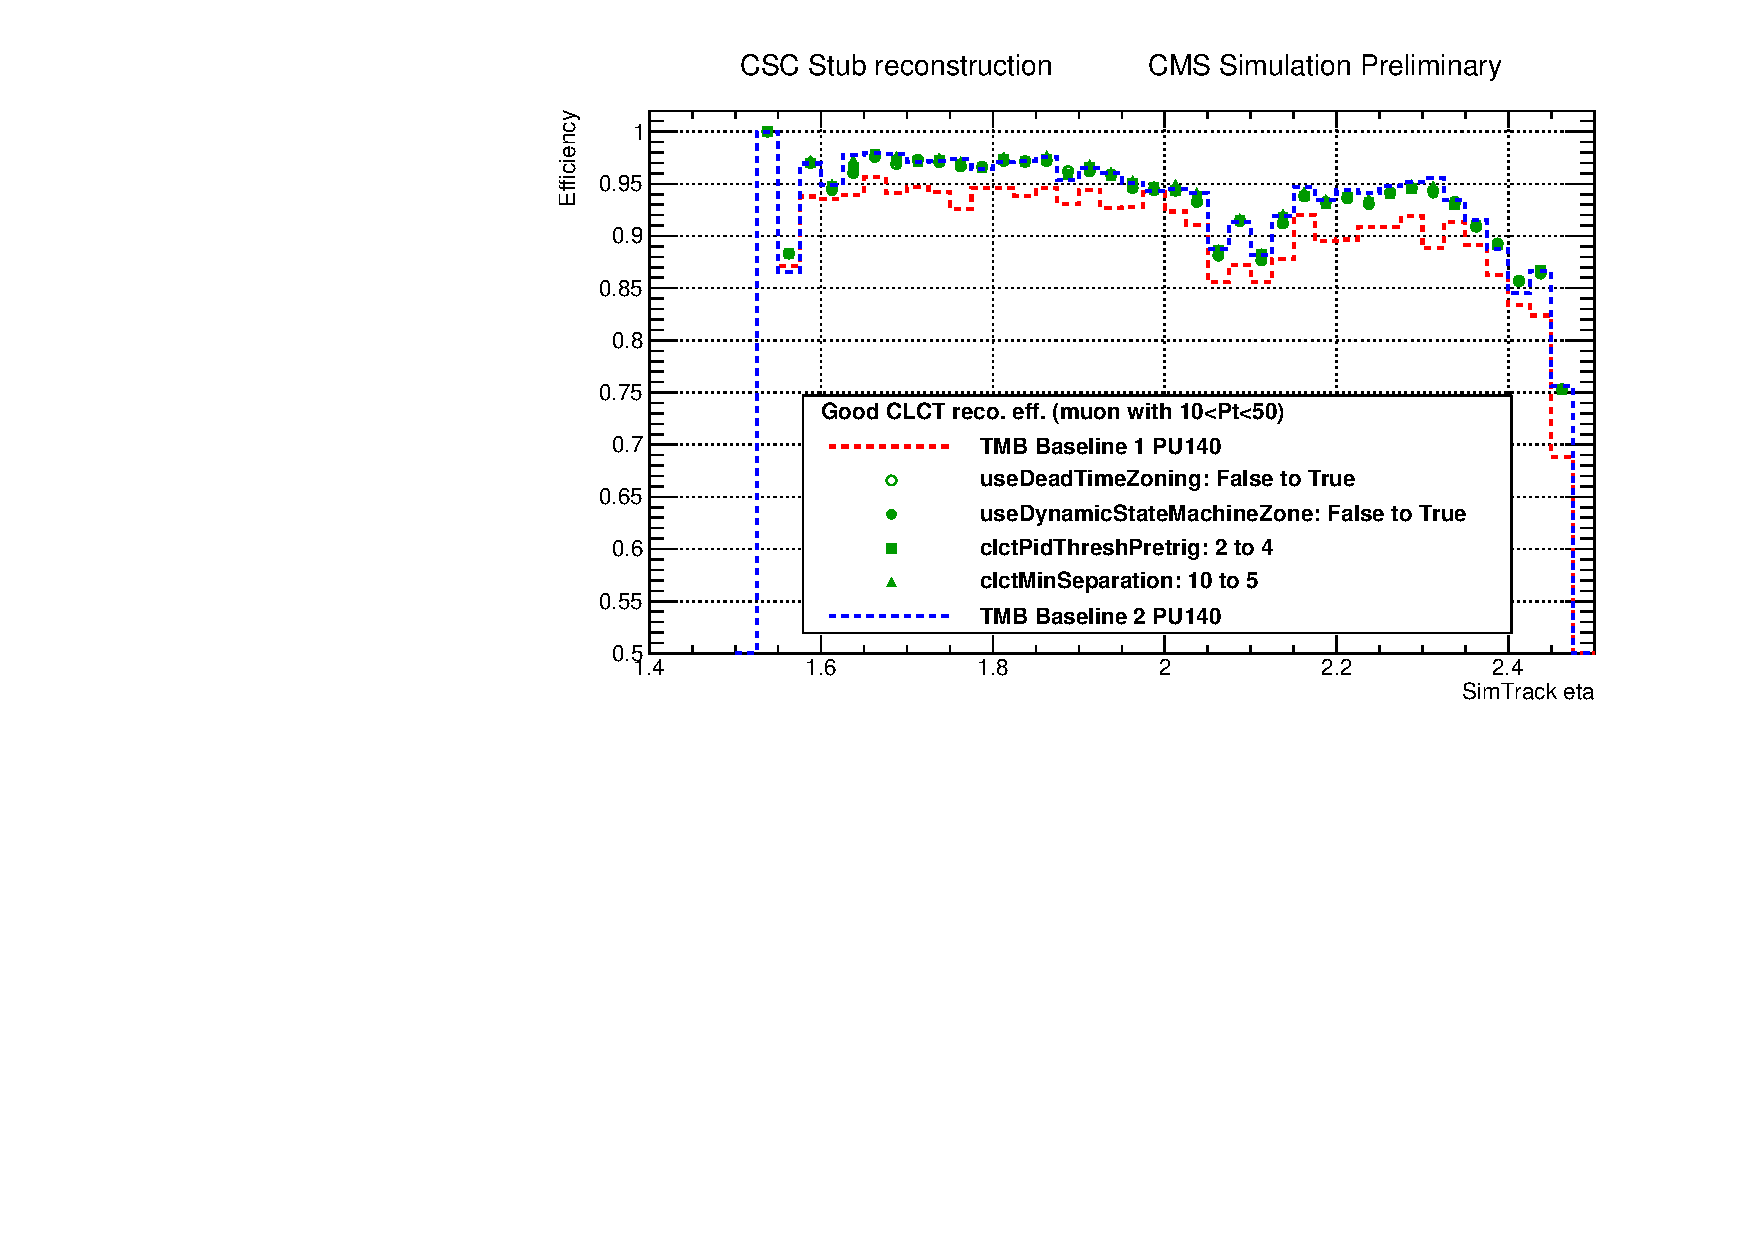
\includegraphics[width=0.98\textwidth]{figures/CLCT_improvements_CLCT_recoEff.pdf}
\caption{Reconstruction efficiency of a good CLCT in ME1 station}
\label{fig:CLCT_improvements_CLCT_recoEff}
\end{figure}

Improvements on the level of CLCT processor are related to the following configuration parameters (see Sec.~\ref{sec:CLCT_conf}):
\begin{itemize}
	\item useDeadTimeZoning: False to True;
	\item useDynamicStateMachineZone: False to True;
	\item clctPidThreshPretrig: 2 to 4;
	\item clctMinSeparation: 10 to 5 cathode strips.
\end{itemize}

Fig.~\ref{fig:CLCT_improvements_CLCT_recoEff} shows reconstruction efficiency of a good CLCT in ME1 station versus pseudorapidity of the simulated muon for different L1 configurations. The good CLCT is defined as CLCT:
\begin{itemize}
        \item read out in the window of 3BX around the central BX (BX6);
        \item reconstructed within 2 cathode strips from the key strip.
	\item has hits at least on three layers
\end{itemize}

The major improvement in CLCT reconstruction efficiency comes from localization of the deadtime zone.

\newpage

\subsection{TMB Level Improvements}

\begin{figure}[htb]
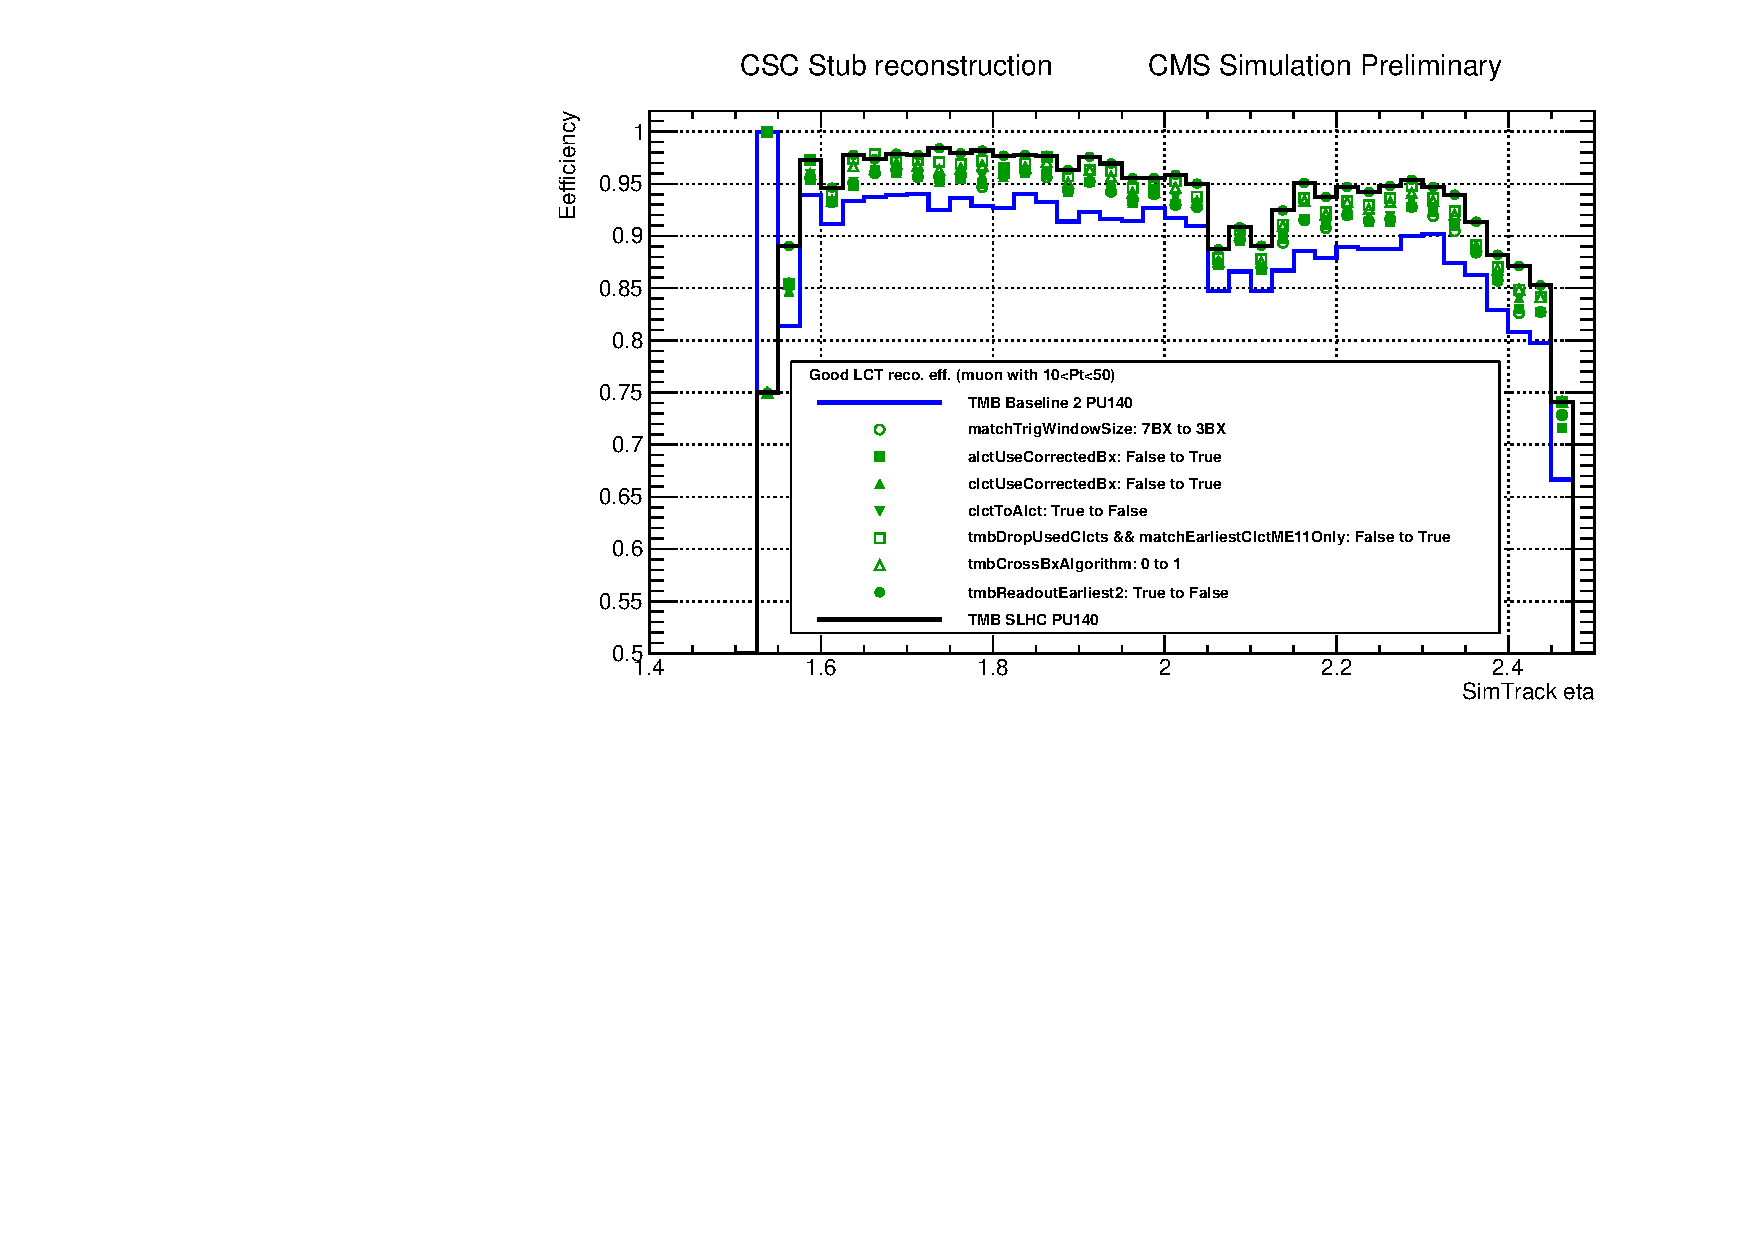
\includegraphics[width=0.98\textwidth]{figures/TMB_improvements_LCT_recoEff.pdf}
\caption{Reconstruction efficiency of a good LCT in ME1 station}
\label{fig:TMB_improvements_LCT_recoEff}
\end{figure}

Improvements on the level of TMB are related to the following configuration parameters (see Sec.~\ref{sec:TMB_conf}):
\begin{itemize}
	\item matchTrigWindowSize: 7BX to 3BX;
	\item tmbReadoutEarliest2: True to False;
	\item alctUseCorrectedBx: False to True
	\item clctUseCorrectedBx: False to True;
	\item clctToAlct: True to False;
	\item tmbDropUsedClcts and matchEarliestClctME11Only: True to False;
	\item tmbCrossBxAlgorithm: 0 to 1.
\end{itemize}

Fig.~\ref{fig:TMB_improvements_LCT_recoEff} shows reconstruction efficiency of a good LCT in ME1 station versus pseudorapidity of the simulated muon for different L1 configurations. The good LCT is defined as LCT consisted of a good ALCT and a good CLCT.

The major improvement in LCT reconstruction efficiency comes from:
\begin{itemize}
	\item changing the size of a window where ALCTs and CLCTs are read out for further correlation betweeb each other;
	\item stopping to read out only the first two CLCTs;
	\item stopping to drop used CLCTs;
	\item stopping to match only to the earliest CLCT.
\end{itemize}

\newpage

\clearpage

\newpage
\tracinginput{sections/algorithm_SLHC_GEM.tex}
%\section{Implementation of a Local Integrated GEM-CSC Trigger for Phase-II Running}
\label{sec:slhc_algorithm_with_gems}

\subsection{The GEM proposal}

\textit{This text here is largely based on Michael Tytgat's introduction of the Conference Proceeding for his contribution in Zaragoza. It's fairly complete, but still too long. Aim for max 20 lines.}

Gas Electron Multipliers (GEMs) are gaseous, position sensitive devices featured by with extraordinary properties: spatial resolutions of order 100 $\mu$m, time resolutions of a few ns, detection efficiencies above 98\% and rate capabilities up to 10 MHz/cm$^2$. They can be operated in a stable manner in high radiation environments, at high gains exceeding $10^4$. %This makes GEMs very suitable detectors for a wide range of applications in many different fields including high energy particle physics. 

The present Muon System contains three different types of detectors for muon tracking and triggering CSCs, RPCs, and DTs. At present, the forward region with 1.6 $<|\eta|<$ 2.4 is only instrumented with CSCs, leaving this part of the detector less robust, with low redundancy for muon tracking and reconstruction. Furthermore, in the foward region one has a relatively high track density, and track projections in the bending plane are relatively short, which hampers the muon momentum determination and makes this area the most challenging region for muon detection. The main issue with respect to muon triggering in this region is the high background rate stemming from low-$p_T$ tracks that are misidentified as high-$p_T$ muons. Adding more detection layers with high granularity at high $|\eta|$ will yield additional space points for track reconstruction to be combined with the information from the CSCs. 

Triple-GEM based detectors are foreseen to be installed in the forward region (1.5 $<|\eta|<$ 2.4) of the muon system. This will improve both the muon momentum resolution and the background rejection at the trigger level, especially in the inner endcap stations where the muon track bending angle due to the magnetic field from the solenoid is largest. Pairs of triple-GEM chambers combined, or super-chambers, will be installed in the two inner endcap stations of the Muon System, as indicated in Fig.~\ref{fig:cms_upg_o_g_b_ni_gem_r_grid_130919}. In the current schedule, the inner endcap stations will be equiped with GEMs (GE1/1) during the second LHC Long Shutdown in 2017-2018, while the installation in the second endcap stations (GE2/1) will be done during the third LHC Long Shutdown scheduled beyond 2020. 

\begin{figure}[tb]
\begin{center}
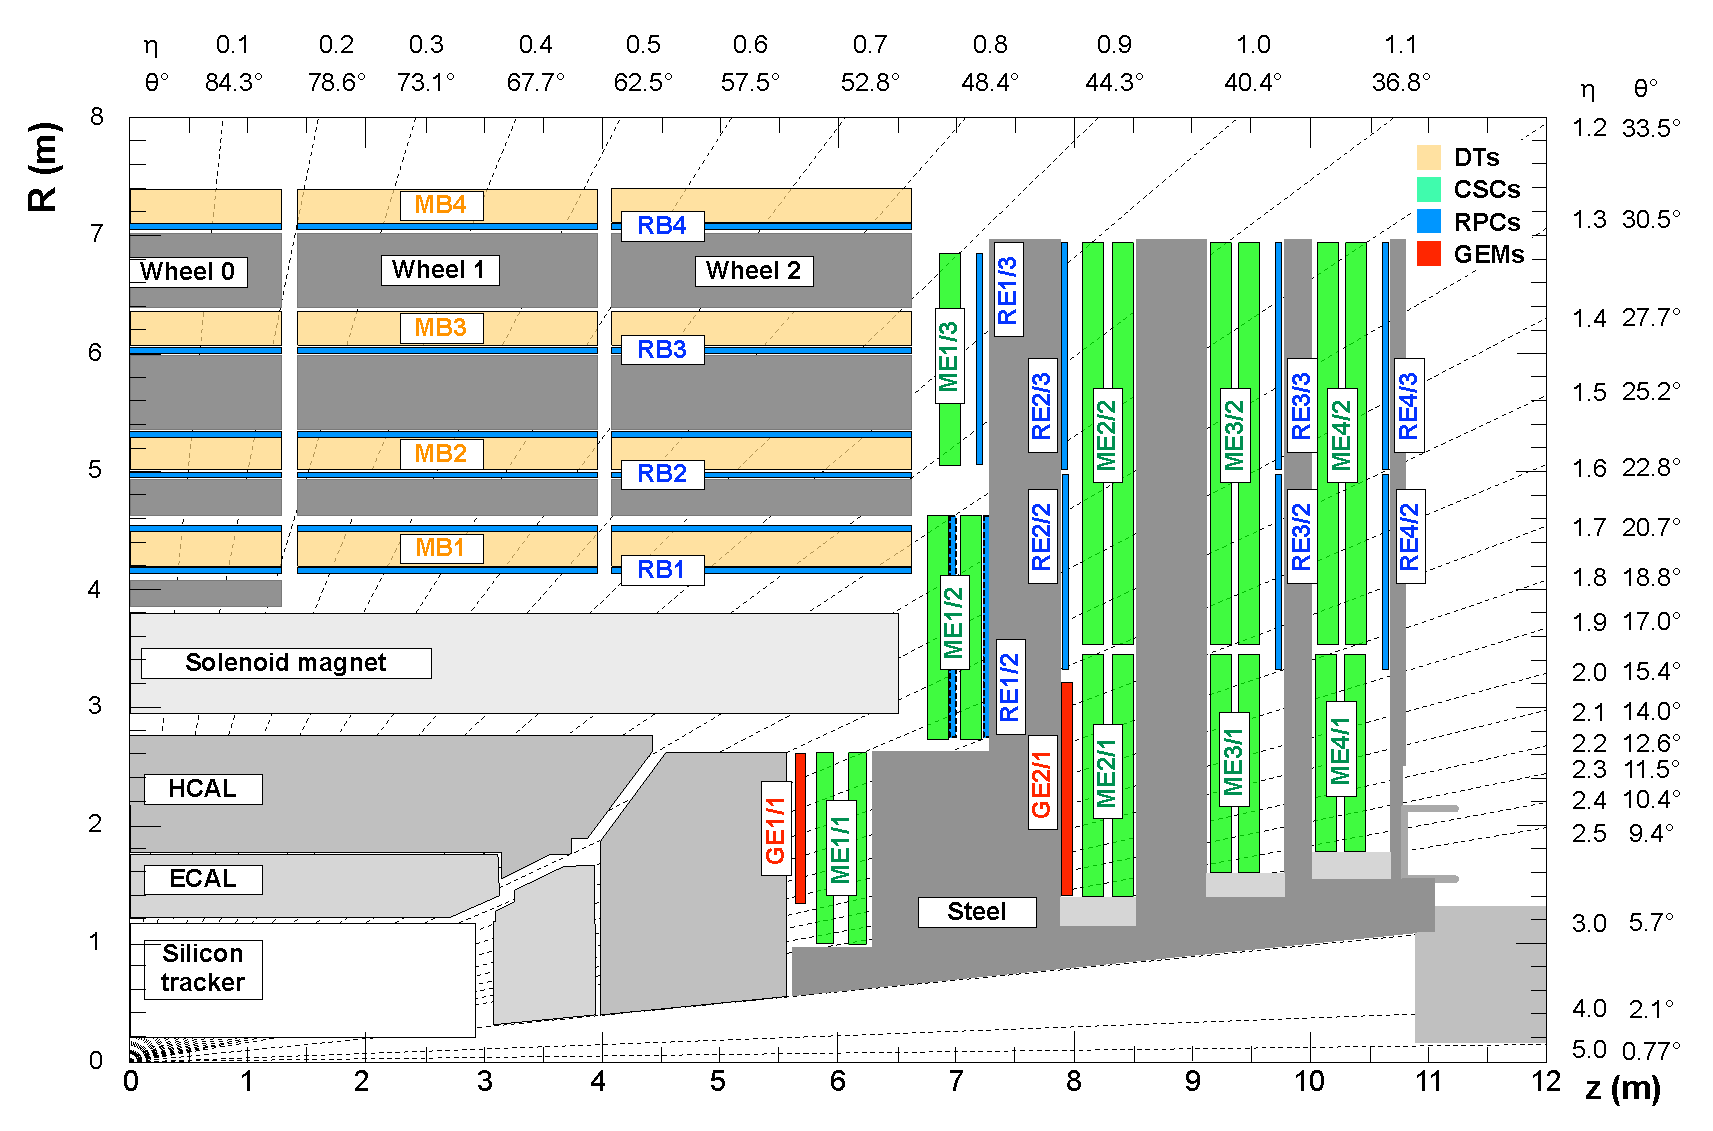
\includegraphics[width=0.9\textwidth]{figures/cms_upg_o_g_b_ni_gem_r_grid_130919.pdf}
\caption{Transverse section of the CMS detector with the foreseen locations of the GE1/1 and GE2/1 station.}
\label{fig:cms_upg_o_g_b_ni_gem_r_grid_130919}
\end{center}
\end{figure}

\subsection{Usage of GEM trigger primitives in the L1 CSC trigger}

\textit{This section is to show that we can use GEMs in the L1 CSC trigger and explain the options to modify the algorithm.}

GEM chambers have 384 strips. GEM digis will be combined in \textsc{OR}'ed combinations of $4$ strips, called GEM-CSC trigger GEM pads or simply pads. The very high efficiency ($>98\%$) results in a nearly $100\%$ efficiency to reconstruct a GEM pad in the first or second layer. This is clearly seen in Fig.~\ref{fig:gem_pad_eff_for_LCT_vs_phi_pt20_overlap}. 

\begin{figure}[htb]
\begin{center}
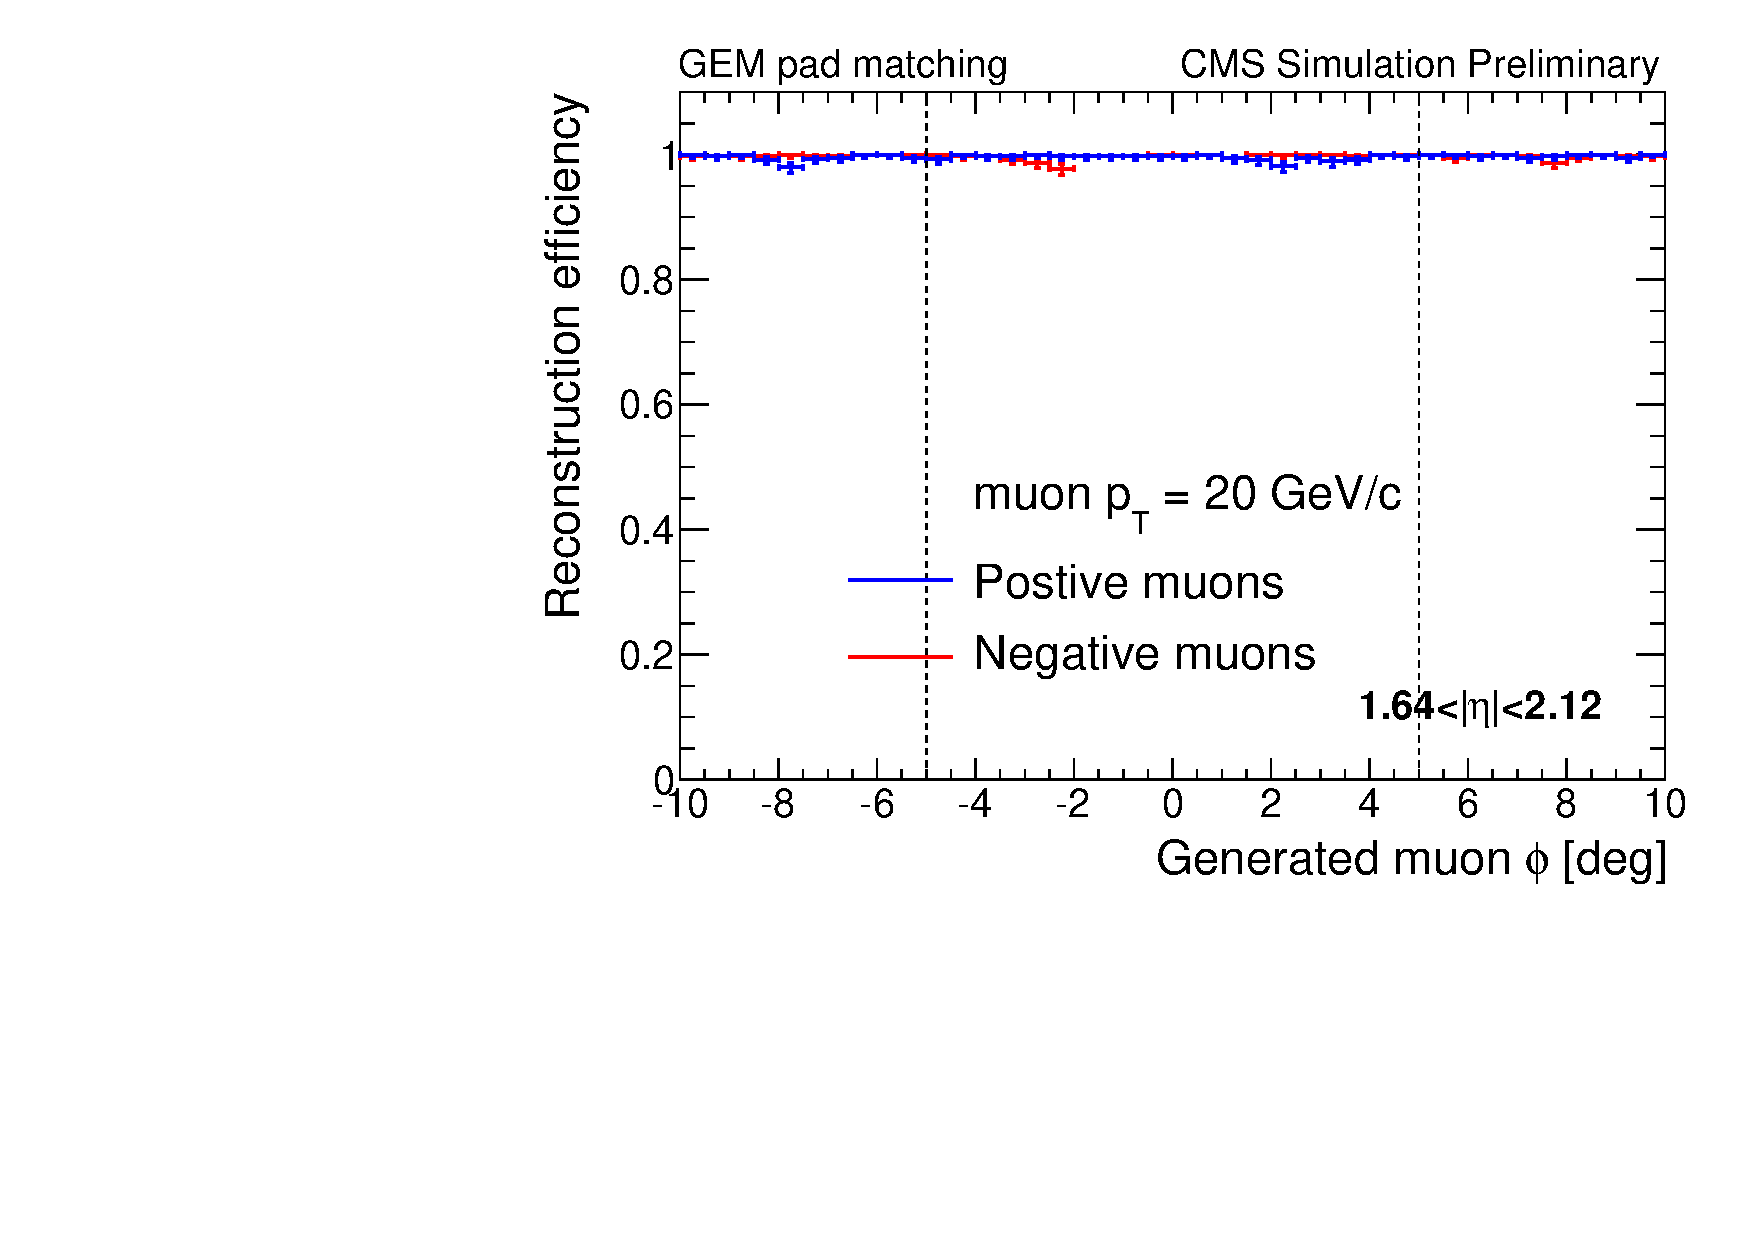
\includegraphics[width=0.5\textwidth]{figures/gem_pad_eff_for_LCT_vs_phi_pt20_overlap.pdf}
\caption{GEM pad reconstruction efficiency versus generated muon phi. The small dips are due to metal spacers in the GE1/1 prototype geometry. These spacers will not be present in the final geometry.}
\label{fig:gem_pad_eff_for_LCT_vs_phi_pt20_overlap}
\end{center}
\end{figure}

In what follows we will investigate several options to reduce the rate and increase the efficiency of the L1 CSC trigger. The first approach is to use the additional GEM information wherever possible in the present CSC trigger algorithm, e.g. to recover misreconstructed ALCTs or CLCTs, to improve the timing, to remove ghost stubs etc. This will be explained in \ref{subsec:slhc_algorithm_with_gems}. The second approach goes much beyond simlpy \textit{patching} up the CSC trigger. It includes reconstructing an LCT from a pair or triplet of ALCT, CLCT and GEM. In that sense a generalization of the definition of a stub in station 1 will be necessary. This will be explained in \ref{subsec:gem_csc_tmb_algorithm}.  
%\textit{Write down where pads are constructed in the hardware and how they are sent to the CSC TMB. Ask Gilles about the details}

\subsection{Factorized GEM-CSC TMB algorithm}
\label{subsec:slhc_algorithm_with_gems}

The factorized GEM-CSC TMB algorithm is aimed to improve the ALCT-to-CLCT matching algorithm and assign the bending angle to be used in the CSC Track Finder. 

The additional information can aid to reduce the rate and improve the efficiency in many ways. A frequent source of ineffiency is the loss of a low-hit ALCT(CLCT) in the CLCT-ALCT(ACLT-CLCT) matching. Whenever there is a GEM coincidence pad the timing of a CLCT(ALCT) can be corrected if necessary. In case a CLCT was missing, a GEM coincidence pad can be used to construct an LCT. In what follows we will investigate the possibility to patch up the CSC ME1/1 algorithm where it is necessary, so called the factorized GEM-CSC TMB algorithm. The other approach is to redesign the algorithm completely. 

\subsubsection{Reduction of soft stubs}
\label{subsubsec:reduction_of_soft_stubs}

As mentioned already in the introduction, a big issue to the present L1 CSC trigger is the flattening of the trigger rate at high $p_T^{cut}$. Low-$p_T$ muons are known to undergo multiple scattering in the iron yoke of the CMS endcap. This scattering causes the stubs to become aligned. As a result, the CSC Track-Finder will see a straight track for the low-$p_T$ muon and will assign a much higher transverse momumentum. If one is able to prevent the soft stubs in station 1 to be used in the track-fit, it will be less likely that a soft muon is given a high $p_T$. 

With the installation of double-layered GEM chambers in station 1, measurement of the bending angle becomes possible. \textit{Add a figure here about the geometrical setup of the bending angle.} Fig.~\ref{fig:GEMCSCdPhi_chambers_reverse} shows the GE1/1-ME1/1 bending angle of 5 GeV and 20 GeV muons in even and odd chambers. The odd chambers show a larger separation of the muons since they are spaced farther apart along the beamline.

\begin{figure}[htb]
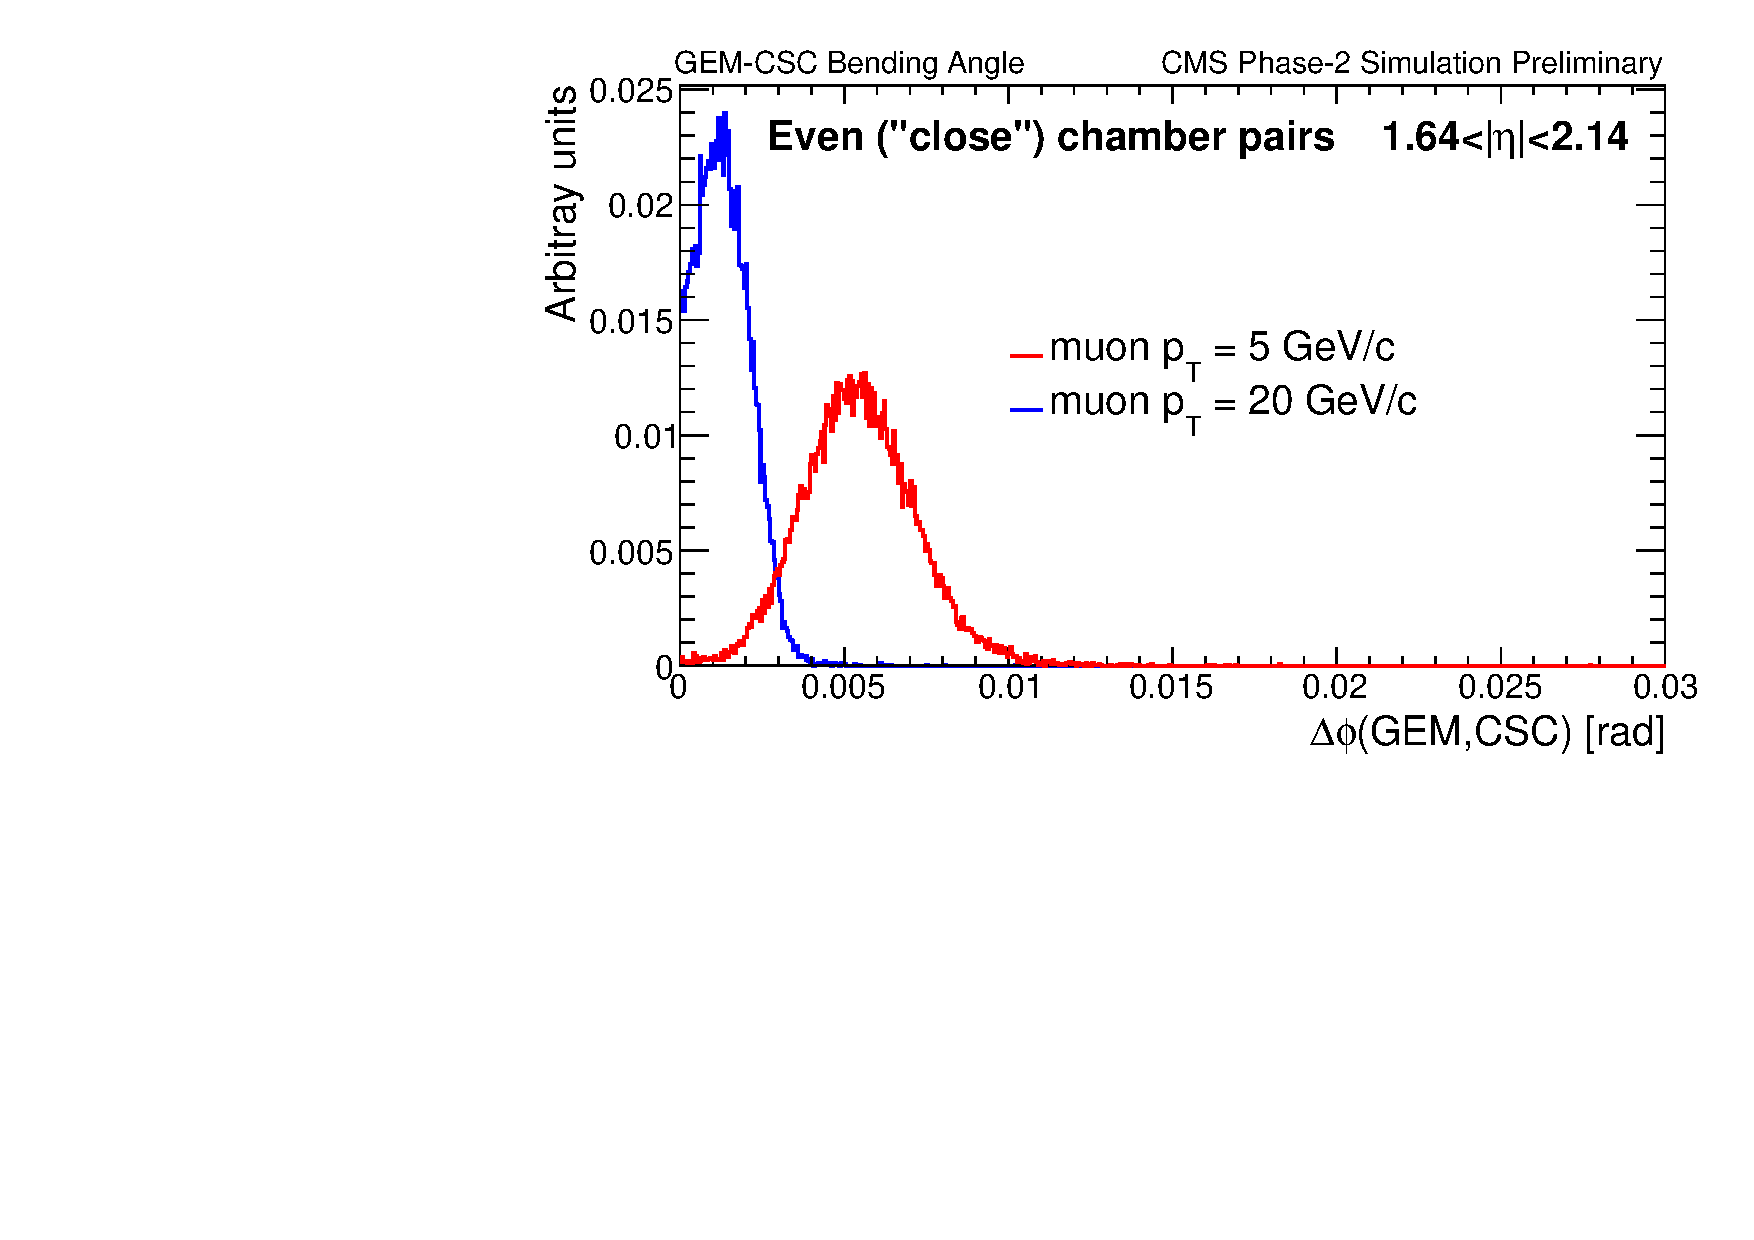
\includegraphics[width=0.5\textwidth]{figures/GEMCSCdPhi_even_chambers_reverse.pdf}
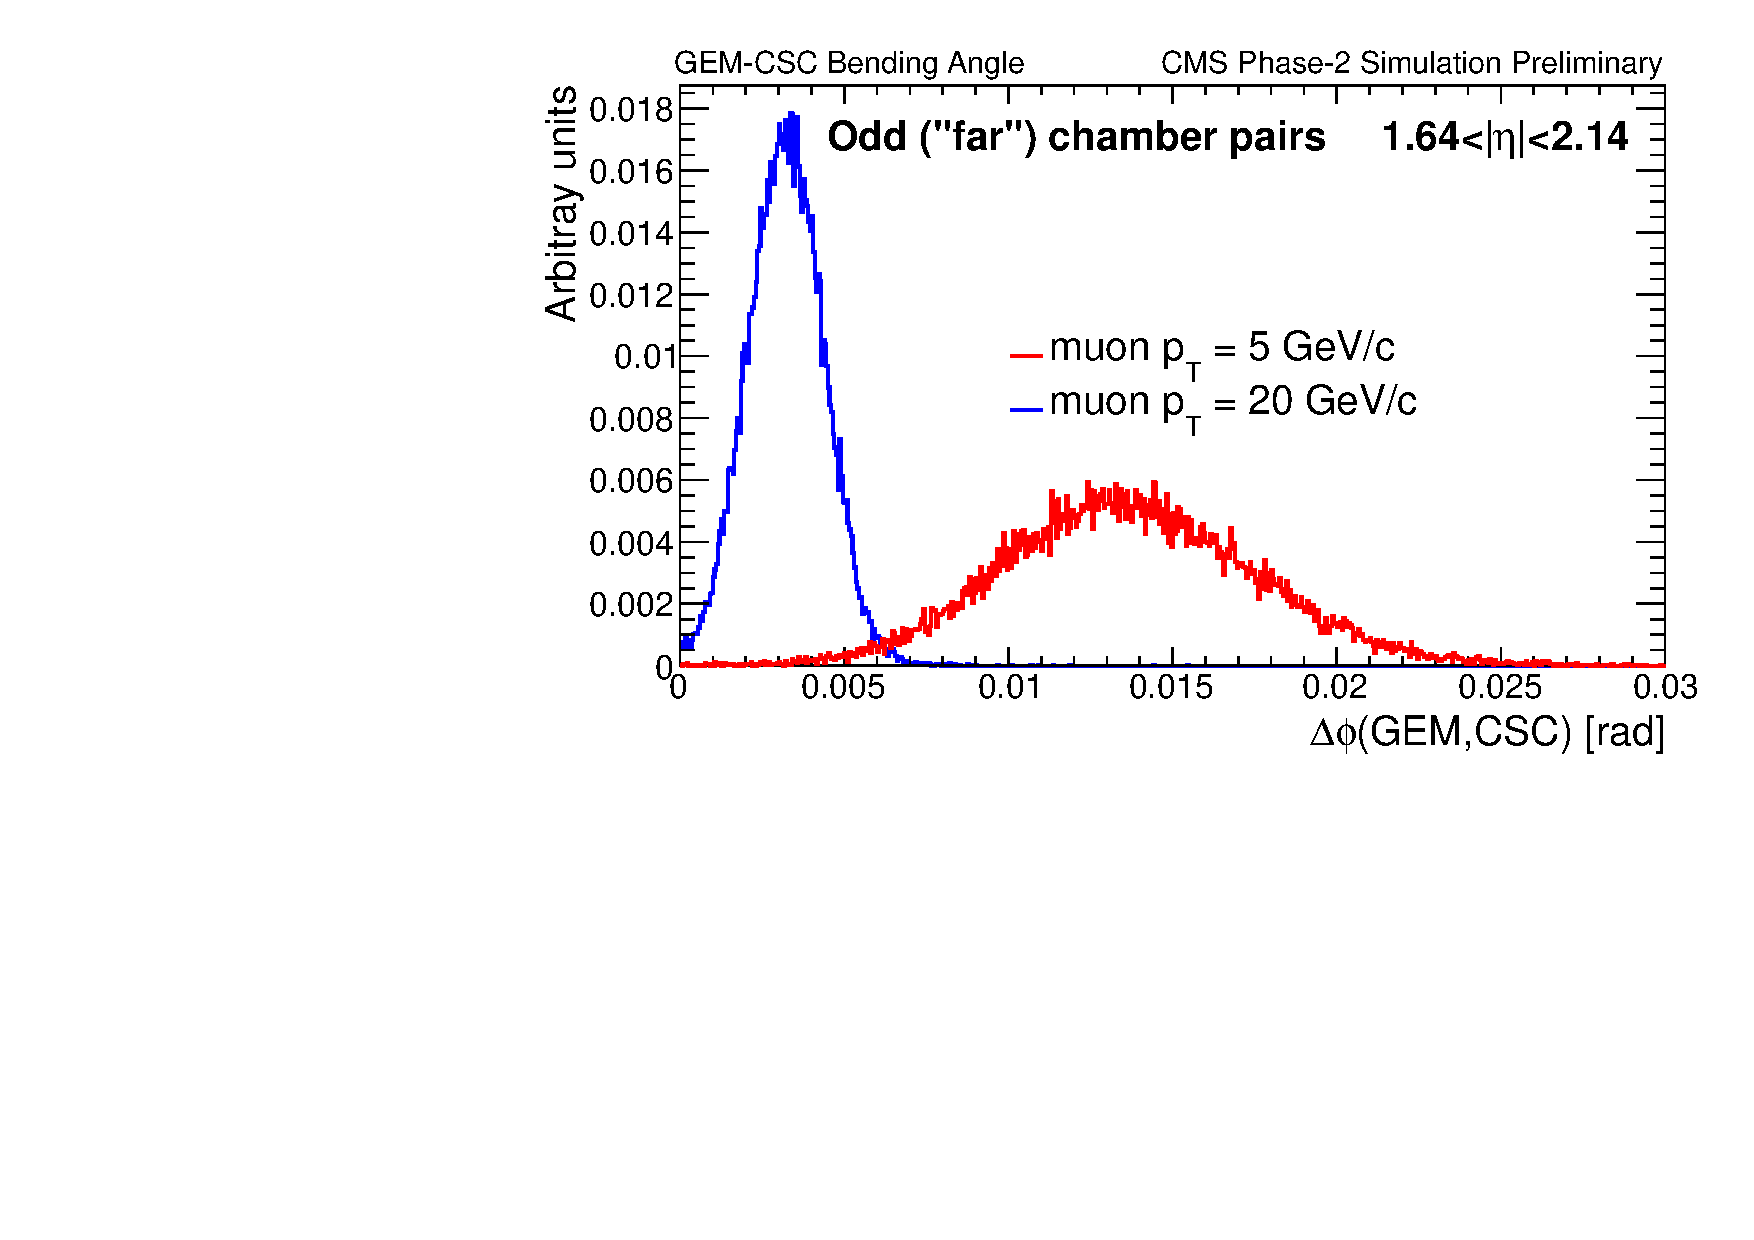
\includegraphics[width=0.5\textwidth]{figures/GEMCSCdPhi_odd_chambers_reverse.pdf}
\caption{Comparison of GEM-CSC bending angle for muons with low pt and high pt for even (left) and odd (right) numbered chambers.}
\label{fig:GEMCSCdPhi_chambers_reverse}
\end{figure}

The discrimination power can now applied in the L1 CSC trigger algorithm. Once the LCTs are reconstructed from an ALCT-CLCT pair via ALCT or CLCT-centric matching, we can try to assign a GEM bending angle to it. First, all GEM trigger pads are collected within the bunch crossing range [5,7], or +1/-1 about the central bunch crossing for a particular LCT. The default value for GEM-CSC bending angle is $-99$. If at least 1 GEM trigger pad is available (SPECFICY), the bending angle is assigned $+99$. To consider a GEM pad as \textit{matched} it has to be within specified \texttt{delta\_eta} and \texttt{delta\_phi} ranges. If there are multiple ones, only the $\min|delta_phi|$ is considered as matched. The unmatched LCTs can be kept or removed. 

To illustrate the effect of this simple pad matching procedure, we ran the modified L1 CSC trigger algorithm for various bending angles corresponding with muon transverse momenta of 5, 6, 10, 15, 20, 30 and 40 GeV. Unmatched LCTs were removed from the event and were not used in the track-fit and Global Muon Trigger. The resulting trigger rate vs $p_T^\text{cut}$ and $\eta$ was calculated by combining the samples. The result is shown in in Fig.~\ref{fig:l1_trigger_rate_csc_gem}. 

\begin{figure}[htb]
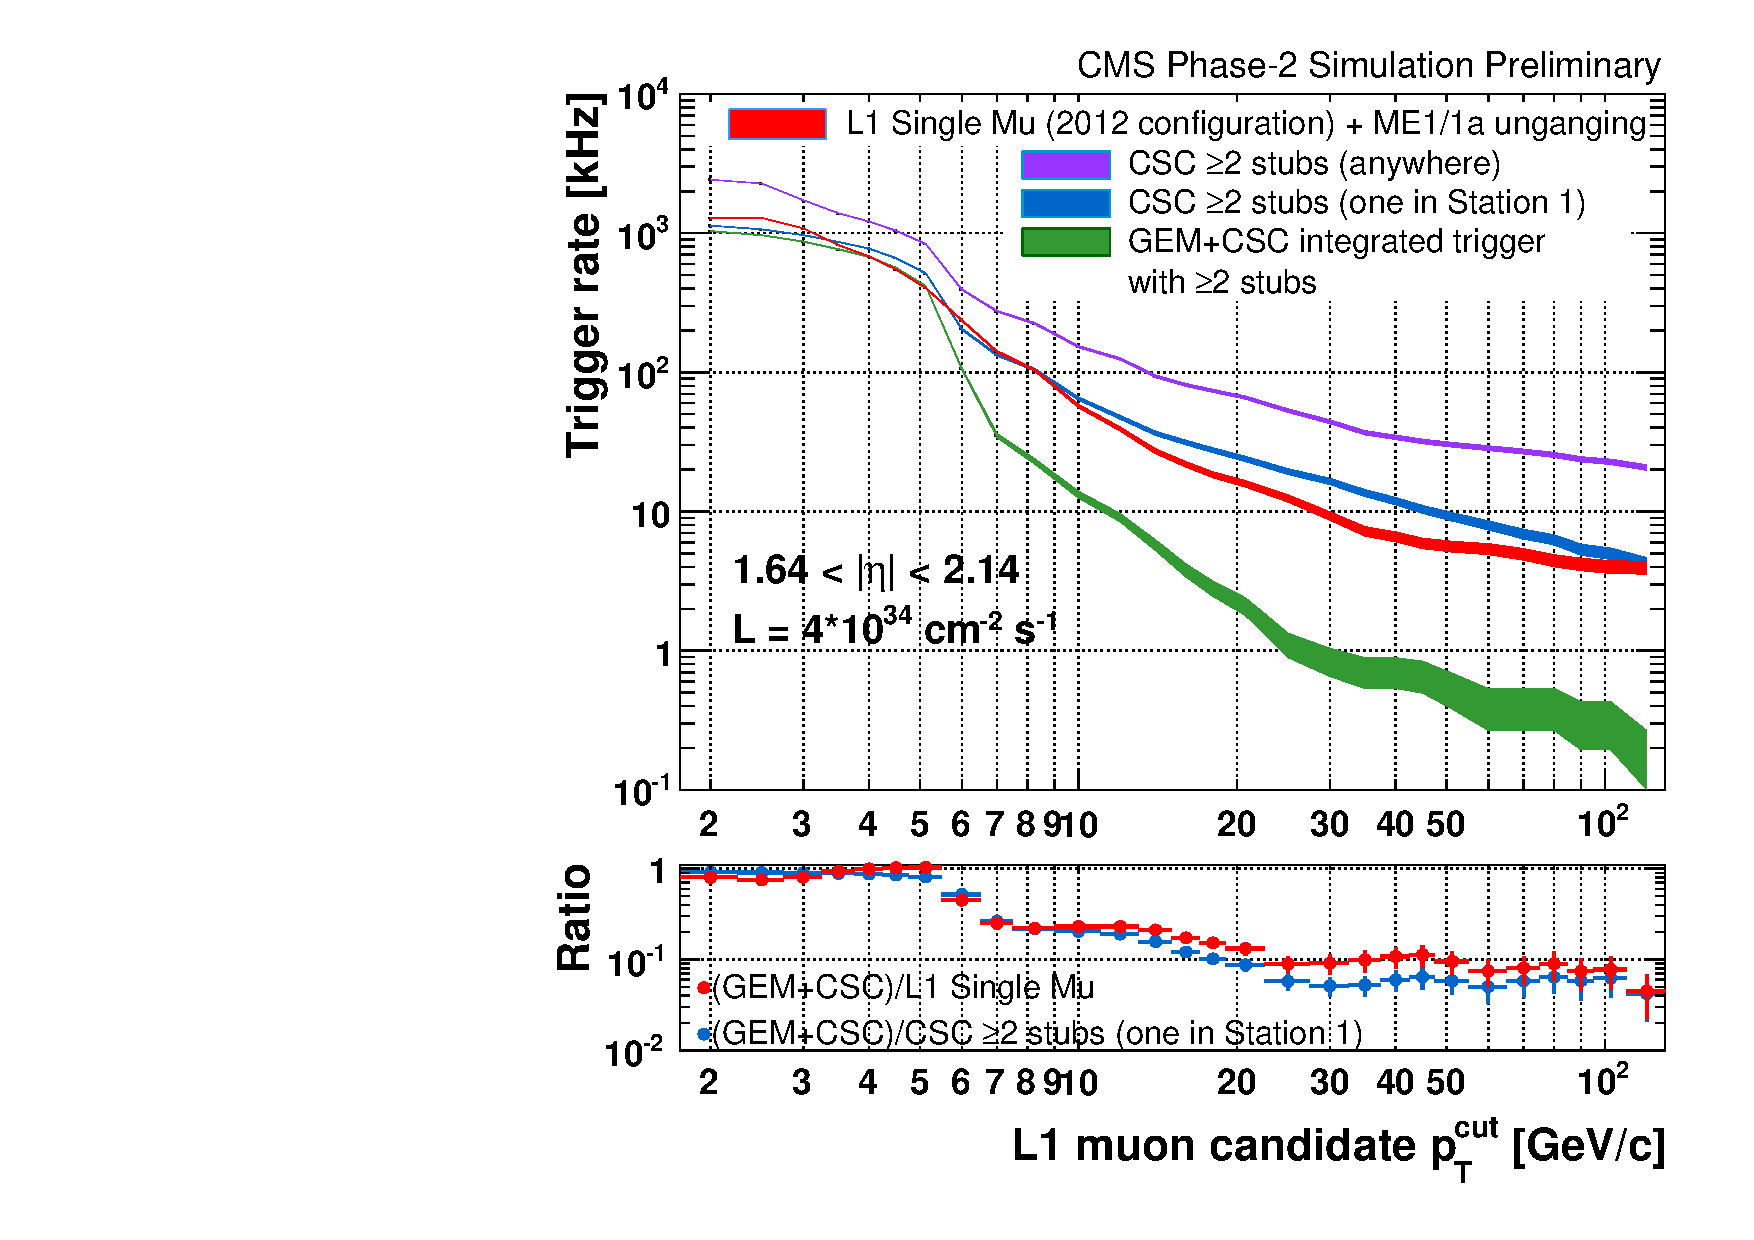
\includegraphics[width=0.5\textwidth]{figures/rates_vs_pt__PU100__def_2s_2s1b_2s1bgem__loose.pdf}
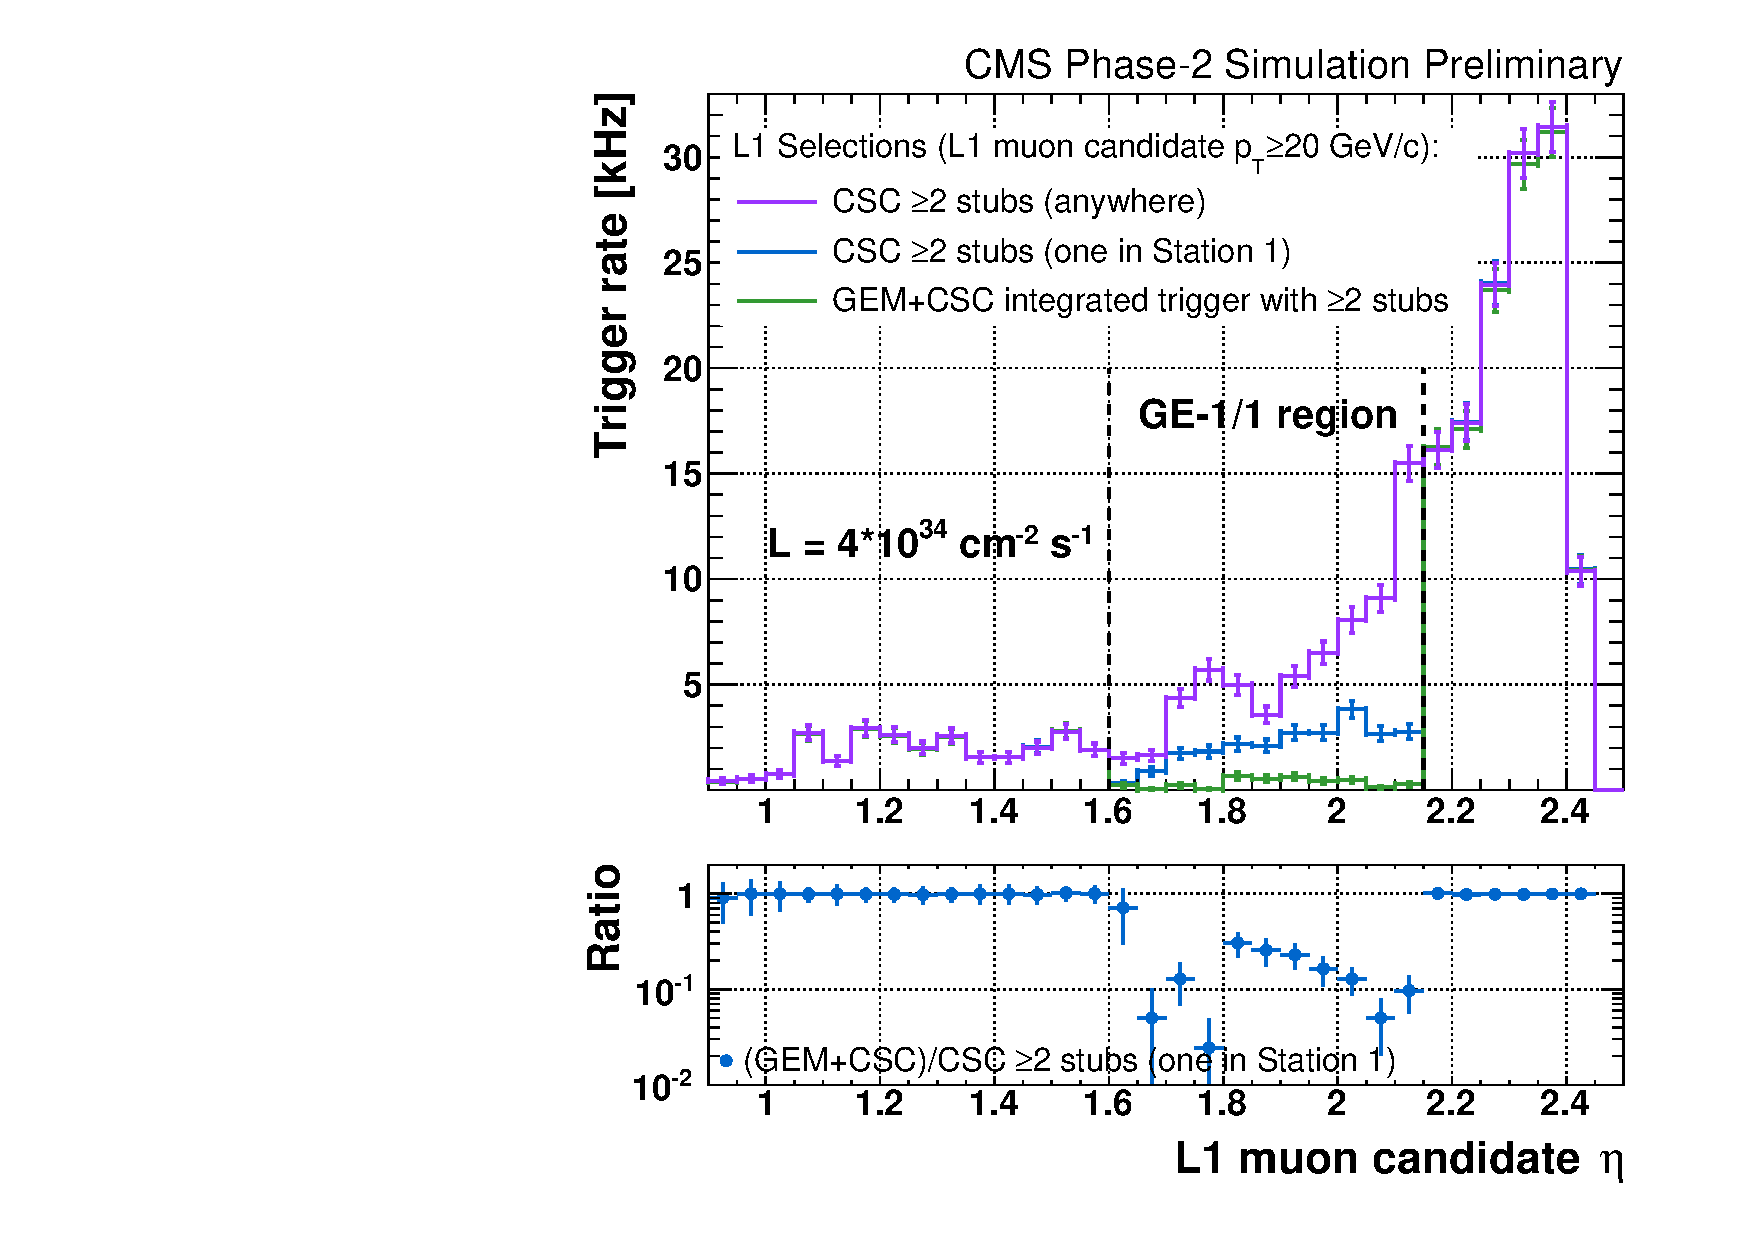
\includegraphics[width=0.5\textwidth]{figures/rates_vs_eta__minpt20__PU100__def_2s_2s1b_2s1bgem.pdf}
\caption{Comparison of the trigger rates (left vs $p_T^\text{cut}$, right vs muon  $\eta$) for the Global Muon Trigger in the 2012 configuration with the CSC Track-Finder track rates for at least 2 stubs (loose), at least 2 stubs with at least one 1 stub from ME1/b (medium), and at least one 2 stubs with at least one 1 stub from ME1/b and a GEM pad (tight). The CSC TF used all patterns. The bottom plot shows the ratio of tight/GMT and tight/medium.}
\label{fig:l1_trigger_rate_csc_gem}
\end{figure}

%\subsubsection{Assignment of the bending angle}
%
%\textit{This is the algorithm as it is currently in software. In firmware there will be no simtrack information and it will be somewhat simpler.}
%
%After the LCTs are reconstructed in the matching step, they can be matched to LCTs. First a check is done if there are any good LCTs at all in the bunch crossing window that is considered. If there are no valid LCTs, no assignment is done. The algorithm will then proceed with a triple-nested loop: on all bunch crossings, on all potential LCT pairs in this bunch crossing, and both LCTs in the pair. 
%
%For each LCT it will start by setting the bending angle to the value $-99$, which is the default value. The CSC trigger geometry is enabled to calculate the position of the LCT int the first CSC layer in the global CMS coordinate system. If the global $\eta$ does not pass the GEM fiduciality requirement, no matching is done. If it does pass the requirement, the bending angle is set to $+99$. The algorithm then proceeds with looping on all trigger pads. For each trigger pad, the global position in the CMS coordinate system is calculated. The bending angle, $\Delta\phi_\text{GEM,CSC}$, is then calculated as $\text{abs}(\phi_\text{GEM}-\phi_\text{CSC})$. The $\Delta\eta$ is calculated from the global position as $\text{abs}(\eta_\text{GEM}-\eta_\text{CSC})$. If $\Delta\eta$ is smaller than the currently fixed value of $0.08$, if  $\Delta\phi_\text{GEM,CSC}$ value is smaller than the $\Delta\phi_\text{GEM,CSC}$ expected for this muon track, and the to now calculated minimum the bending angle is stored in the dataformat. Using a look-up-table the bending angle is converted to a bit-wise value. 

\subsubsection{Low-hit stub recovery in ALCT-CLCT matching}

\textit{First part of this subsection is about ALCT-CLCT. Second part are the results for CLCT-ALCT.}

A frequent source of inefficiency is when insufficient strip layers were hit within 4 BX to form a CLCT. The current conditions for a CLCT to pass the pre-trigger and trigger requirement are 3/6 and 4/6 respectively. On the one hand, one can reduce the trigger requirement of 4/6 to 3/6 layers. One the other hand, the introduction of a double-layered GEM system effectively increases the number of layers from 6 to 8. The CLCT reconstruction efficiency should go up if we require 4/8 instead of 4/6 layers. The results of this are show in Fig. for two different high pile-up scenarios.

\textit{Make two plots: PU140 and PU400 for fixed pre-trigger of 3 and trigger of 3/6, 4/6 and 4/8} 

\begin{figure}[htb]
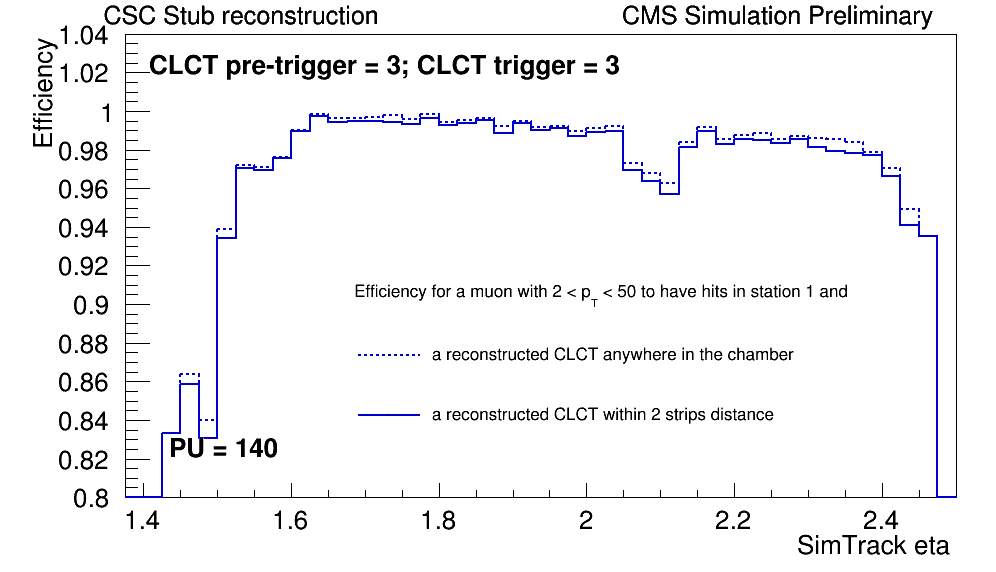
\includegraphics[width=0.5\textwidth]{figures/simTrackToClctMatchingEfficiencyVsEtaME1_pu140_preTrig33.png}
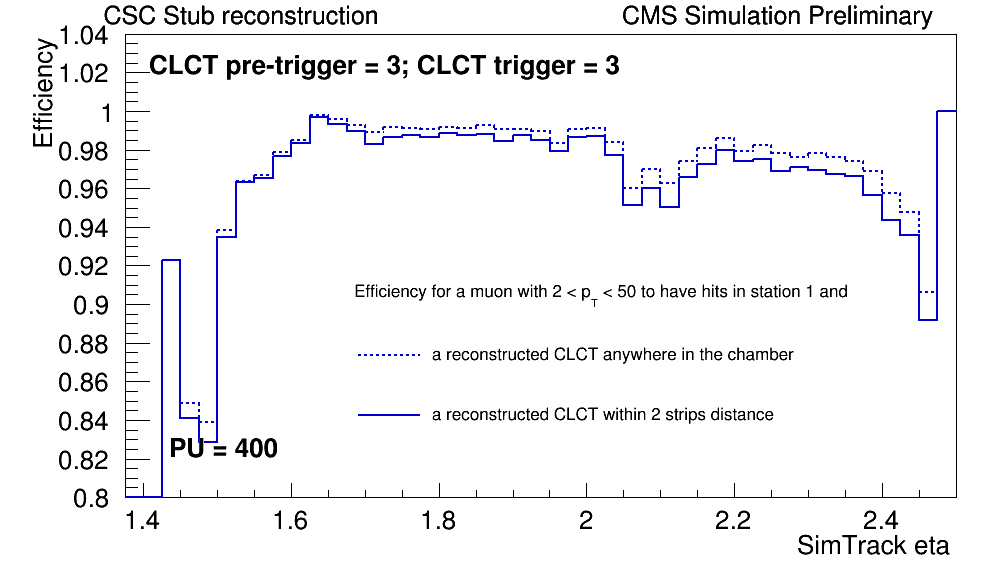
\includegraphics[width=0.5\textwidth]{figures/simTrackToClctMatchingEfficiencyVsEtaME1_pu400_preTrig33.png}
\caption{CLCT reconstruction efficiency for a pre-trigger and trigger requirement of 3 for several pile-up scenarios.}
\label{fig:clct_reconstruction_efficiency_eta_trig_pu}
\end{figure}

\textit{Add here the plots for CLCT-ALCT matching.}

\subsubsection{Disambiguation of best and second best stub}

\subsubsection{Substitution of a GEM for an ALCT/CLCT in the matching}

As explained in section (REFERENCE) the upper and lower part of the ME1/1 chamber, called ME1/b and ME1/a respectively have a separate CFEBs to process the comparator digis. This has far-reaching consequences, in particular for muons going through the overlap region or through the edges of the chamber. If a muon goes through the overlap region, it may have hit at least 4 layers hit in the whole ME1/1 chamber, but may not have enough hits in either sub-chamber to pass the pre-trigger and trigger requirement. An example is the case: 3 layers hit in ME1/b and 2 layers hit in ME1/a. 

In case the other ME1/1 stub was not reconstructed, one can make an attempt to form an LCT out of the available ME1/1 stub and a GEM coincidence pad.

\textit{Construction of coincidence pads in the TMB. Make a separate section or not?}

%\subsubsection{Construction of GEM coincidence pads}

T
After the ALCTs and CLCTs are retrieved from the corresponding processors, the GEM pads from the neighbouring GE1/1 chambers are collected. The GEM pads will be assigned a chamber number, a roll number, a pad number and a bunch crossing. The current definition of a coincidence pad is as follows:
\begin{itemize}
\item Pad 1 comes from chamber 1
\item Pad 2 comes from chamber 2
\item Both pads have the same pad number
\item Both pads have the same eta partition number
\item The time of pad 1 and pad2 can differ by at most 1 bunch crossing
\end{itemize}


Suppose that in the ALCT centric matching no good CLCT was found within the bunch crossing window, one can use substitute a GEM coincidence pad, provided it was found, for a CLCT. This requires a more general definition of an LCT.  

%\textit{Go in more details about the definition of a GEM pad}
%
%Of course, the current definition is subject to improvement to allow for various cases that can still be regarded as a coincidence pad. For instance, a muon hitting a GEM on the edge of two eta partitions in the first chamber could hit the eta partition above below (depending how it was going. A second case is where a muon hit a GEM chamber on the edge of certain pad in the first chamber. In this case it could go through a pad with a pad higher or lower number in the second chamber. In the future one could go for an extended definition more extended version of a GEM pad to allow for such cases.  

%\subsubsection{Wrapping of pads and co-pads}
%
%\textit{Figure out how the GEM pads are encoded in the data. Maybe it does not have to be done in firmware.}



\subsubsection{Correction of stub timing}





\subsection{Future algorithm with additional improvements}

The following is an overview of the algorithm 

\begin{enumerate}
\item Retrieve the ALCTs from the ALCT processor board
\item Reconstruct the CLCTs in the CLCT processor board for ME1/b
\item Reconstruct the CLCTs in the CLCT processor board for ME1/a
\item Stub matching procedure.
\begin{itemize}
\item CLCT-to-ALCT matching
\item ALCT-to-CLCT matching
\begin{enumerate}
\item For each bunch crossing in the maximum number of ALCT BXs check if the ALCT has a valid pattern
\item Check if there are any trigger pads and co-pads
\item For each CLCT in the CLCT matching BX window, check if the CLCT has a valid pattern
\item If the CLCT has less than 4 layers hit and if there was no trigger pad, continue with the next CLCT. 
\item Correlate the best CLCT with the best ALCT and the second best CLCT with the second best ALCT.
\end{enumerate}
\end{itemize}
\item Assignment of the GEM-CSC bending angle. 
\item Reduction of the number of LCTs 
\end{enumerate}

\subsubsection{GEM-CSC TMB algorithm}
\label{subsec:gem_csc_tmb_algorithm}

The second option goes beyond patching up the existing improved ME1/1 algorithm. In this algorithm we consider the ALCT, CLCT and GEM and perform a sort of voting to construct a more general LCT with 3 different LCT classes
\begin{itemize}
\item ALCT and CLCT
\item ALCT and GEM
\item CLCT and GEM
\end{itemize}
In case one has ALCT, CLCT and GEM, only the two highest quality stubs are chosen to reconstruct the LCT. Evidently, this change in object definition goes together with a change in dataformat. 

\subsubsection{Future possibilities for GEM-CSC triggering}
\label{subsec:future_possibilities_for_gem_csc_triggering}

\textit{Write something here about GE2/1-ME2/1 trigger options}

\textit{Write something here about ME0 trigger options}

\newpage

\clearpage

% >> acknowledgements (for journal papers)
% Please include the latest version from https://twiki.cern.ch/twiki/bin/viewauth/CMS/Internal/PubAcknow.
%\section*{Acknowledgements}
% ack-text

%% **DO NOT REMOVE BIBLIOGRAPHY**
\bibliography{auto_generated}   % will be created by the tdr script.
%% Customizable fields and text areas start with % >> below.
% Lines starting with the comment character (%) are normally removed before release outside the collaboration, but not those comments ending lines

% svn info. These are modified by svn at checkout time.
% The last version of these macros found before the maketitle will be the one on the front page,
% so only the main file is tracked.
% Do not edit by hand!
\RCS$Revision: 274820 $
\RCS$HeadURL: svn+ssh://tahuang@svn.cern.ch/reps/tdr2/notes/DN-13-022/trunk/DN-13-022.tex $
\RCS$Id: DN-13-022.tex 274820 2015-01-24 00:27:49Z pakhotin $
%%%%%%%%%%%%% local definitions %%%%%%%%%%%%%%%%%%%%%
% This allows for switching between one column and two column (cms@external) layouts
% The widths should  be modified for your particular figures. You'll need additional copies if you have more than one standard figure size.
\newlength\cmsFigWidth
\ifthenelse{\boolean{cms@external}}{\setlength\cmsFigWidth{0.85\columnwidth}}{\setlength\cmsFigWidth{0.4\textwidth}}
\ifthenelse{\boolean{cms@external}}{\providecommand{\cmsLeft}{top}}{\providecommand{\cmsLeft}{left}}
\ifthenelse{\boolean{cms@external}}{\providecommand{\cmsRight}{bottom}}{\providecommand{\cmsRight}{right}}
%%%%%%%%%%%%%%%  Title page %%%%%%%%%%%%%%%%%%%%%%%%
\cmsNoteHeader{DN-13-022} % This is over-written in the CMS environment: useful as preprint no. for export versions
% >> Title: please make sure that the non-TeX equivalent is in PDFTitle below
\title{Improvements to ME1/1 Trigger Motherboard Algorithm for Operation under High Pile-Up Running Conditions}

% >> Authors
%Author is always "The CMS Collaboration" for PAS and papers, so author, etc, below will be ignored in those cases
%For multiple affiliations, create an address entry for the combination
%To mark authors as primary, use the \author* form
\address[ghent]{Ghent University}
\address[tamu]{Texas A\&M University}
\address[ucla]{University of California, Los Angeles}
\address[osaka]{University of Seoul}
\address[ufl]{Univerosity of Florida}
\author[ghent]{Sven Dildick}
\author[tamu]{Jose Roberto Dimas Valle}
\author[ucla]{Jay Hauser}
\author[tamu]{Tao Huang}
\author[tamu]{Vadim Khotilovich}
\author[tamu]{Vyacheslav Krutelyov}
\author[osaka]{Jason Lee}
\author[ufl]{Alexander Madorsky}
\author[tamu]{Yuriy Pakhotin}
\author[ucla]{Andrew Peck}
\author[tamu]{Alexei Safonov}
\author[tamu]{Aysen Tatarinov}
\author[ucla]{Vyacheslav Valuev}

% >> Date
% The date is in yyyy/mm/dd format. Today has been
% redefined to match, but if the date needs to be fixed, please write it in this fashion.
% For papers and PAS, \today is taken as the date the head file (this one) was last modified according to svn: see the RCS Id string above.
% For the final version it is best to "touch" the head file to make sure it has the latest date.
\date{\today}

% >> Abstract
% Abstract processing:
% 1. **DO NOT use \include or \input** to include the abstract: our abstract extractor will not search through other files than this one.
% 2. **DO NOT use %**                  to comment out sections of the abstract: the extractor will still grab those lines (and they won't be comments any longer!).
% 3. For PASs: **DO NOT use tex macros**         in the abstract: CDS MathJax processor used on the abstract doesn't understand them _and_ will only look within $$. The abstracts for papers are hand formatted so macros are okay.
\abstract{
Improvements to ME1/1 trigger motherboard algorithm for operation under high pile-up conditions are described as well as details of their configuration in software. Individual effects of these improvements on ME1/1 trigger efficiency are quantified and ranked in terms of their importance in simulation studies.
}

% >> PDF Metadata
% Do not comment out the following hypersetup lines (metadata). They will disappear in NODRAFT mode and are needed by CDS.
% Also: make sure that the values of the metadata items are sensible and are in plain text:
% (1) no TeX! -- for \sqrt{s} use sqrt(s) -- this will show with extra quote marks in the draft version but is okay).
% (2) no %.
% (3) No curly braces {}.
\hypersetup{%
pdfauthor={Aysen Tatarinov},%
pdftitle={Improvements to ME1/1 Trigger Motherboard Algorithm for Operation under High Pile-Up Running Conditions},%
pdfsubject={CMS},%
pdfkeywords={LHC, CMS, Muons, CSC, Trigger}}

\maketitle %maketitle comes after all the front information has been supplied
% >> Text
%%%%%%%%%%%%%%%%%%%%%%%%%%%%%%%%  Begin text %%%%%%%%%%%%%%%%%%%%%%%%%%%%%
%% **DO NOT REMOVE THE BIBLIOGRAPHY** which is located before the appendix.
%% You can take the text between here and the bibiliography as an example which you should replace with the actual text of your document.
%% If you include other TeX files, be sure to use "\input{filename}" rather than "\input filename".
%% The latter works for you, but our parser looks for the braces and will break when uploading the document.

\tableofcontents

\newpage
\tracinginput{sections/introduction.tex}
%\section{Introduction}

The muon trigger is a tracking trigger that measures the momentum of muons using the magnetic field in the steel yoke of the CMS detector~\cite{Chatrchyan:2008zzk}; thus its resolution degrades with increasing momentum. This can be improved by maximizing the number of chamber hits along a muon trajectory and by improving the precision and number of position and angular measurements participating in the track fit applied in the trigger logic. The focus of the muon trigger upgrade is to improve its rate reduction capability without significantly affecting the efficiency.

The philosophy applied to the design of the present muon trigger was to preserve the complementarity and redundancy of the three separate muon detection systems until they are combined at the input to the Global Trigger. In contrast, the upgrade to the muon trigger will utilize the redundancy of the three muon detection systems earlier in the trigger processing chain so as to obtain a more performant trigger with higher efficiency and better rate reduction. Recognizing that every additional hit along a muon trajectory further improves the fake rejection and muon momentum measurement, the upgrade seeks to combine muon hits at the input stage to the Muon Track-Finder layer rather than at its output, given the successful operation of all three muon detection systems in the LHC Run 1. This new Muon Track-Finder will ultimately replace the separate track-finders for the Drift-Tube (DT) and Cathode Strip Chamber (CSC) muon triggers as well as the Resistive Plate Chamber (RPC) pattern comparator trigger. However, in addition to combining data from multiple muon systems in the same processors, more robust and sophisticated algorithms will be applied that are tolerant of the increased pile-up and make better use of the data from each muon system in the track-finding and $p_T$ measurement. Present and upgraded muon trigger algorithms in CSC are described in Section~\ref{sec:present_algo} and Section~\ref{sec:SLHC_algo}, correspondingly. Individual improvements of the upgraded algorithm are studied in Section~\ref{sec:SLHC_algo_results}.

The muon trigger upgrade is not expected to be completed before the LHC resumes operation after Long Shutdown I in 2015. Thus it is imperative to be able to commission the new muon trigger in parallel with the operation of the current trigger. For that reason, the trigger primitives from the CSC and RPC systems will be fully split into two paths, and those from the DT system will be split from a slice of the system. Data concentration into high bandwidth links for all three systems should be available for at least a slice of the detector as input to the new trigger in 2015. The goal is to have the entire muon trigger upgrade commissioned during the 2015-16 Year-End Technical Stop, so that the new trigger will be available in 2016. Recognizing the physics importance of the first year of LHC running at a higher center-of-mass energy ($\sqrt{s} = 13$~TeV) in 2015, a provision is foreseen to apply isolation criteria to the CSC muons in the forward region of the detector using the energy deposits in the calorimeter. This will allow to maintain relatively low $p_T$ thresholds reducing the rate of muons from heavy flavor jets despite the higher collision energy and higher luminosity.

As a part of future upgrade for Phase II of LHC running, the CMS will be equiped with Gas Electron Multiplier (GEM) detectors in the high pseudorapidity region ($1.5 < |\eta| < 2.2$). Pairs of triple-GEM chambers will be installed in the currently vacant position in front of the ME1/1 chambers and are dubbed GE1/1. The addition of such chambers allows to measure the bending angle of a track between GE1/1 and ME1/1. Usage of the bending angle at L1 can help to keep the rates down while keeping the efficiency high. In section \ref{sec:slhc_algorithm_with_gems} we investigate several implementation possibilities of the combined GEM-CSC trigger algorithm for the high luminosity run of SLHC.
\clearpage

\newpage
\tracinginput{sections/muon_trigger.tex}
%\section{Present Muon Trigger}

\subsection{Global Trigger Data-Flow}

Each of the three muon detector systems in CMS participates in the Level-1 (L1) muon trigger for coverage and redundancy. For the DT and CSC systems ($|\eta|$ $<$ 1.2 and $|\eta|$ $>$ 0.9, respectively), the front-end trigger primitive generator (TPG) electronics identify track segments from the hit information registered in multiple gas planes of a single measurement station. These segments are collected and then transmitted via optical fibres to regional Track-Finders in the electronics service cavern, which then apply pattern recognition algorithms in order to identify muon candidates and measure their momenta from the magnetic bending in the return yoke between several measurement stations. Information is shared between the DT Track-Finder (DTTF) and CSC Track-Finder (CSCTF) for efficient coverage in the region of overlap between the two systems at $|\eta|$ $\approx 1$. The hits from the RPC system ($|\eta|<1.6$) are directly sent from the front-end electronics to Pattern Comparator (PAC) logic boards that identify muon candidates.

The three regional track-finders sort the identified muon candidates and transmit to the Global Muon Trigger (GMT) up to 4 (CSCTF, DTTF) or 8 (RPC) candidates every bunch crossing. Each candidate has been assigned a $p_T$ and quality code as well as $\eta$ and $\phi$ positions in the muon system (with a granularity of $\approx 0.05$). The GMT then merges muon candidates found by more than one system to eliminate fake multi-muon triggers (with several options on how to select $p_T$ between the candidates), and can suppress muon candidates in some regions of the detector if their quality is low and they are unconfirmed by another muon detector system. The data flow of the present L1 muon trigger is shown in Fig.~\ref{fig:l1_muon_trig}.

\begin{figure}[b]
	\begin{center}
		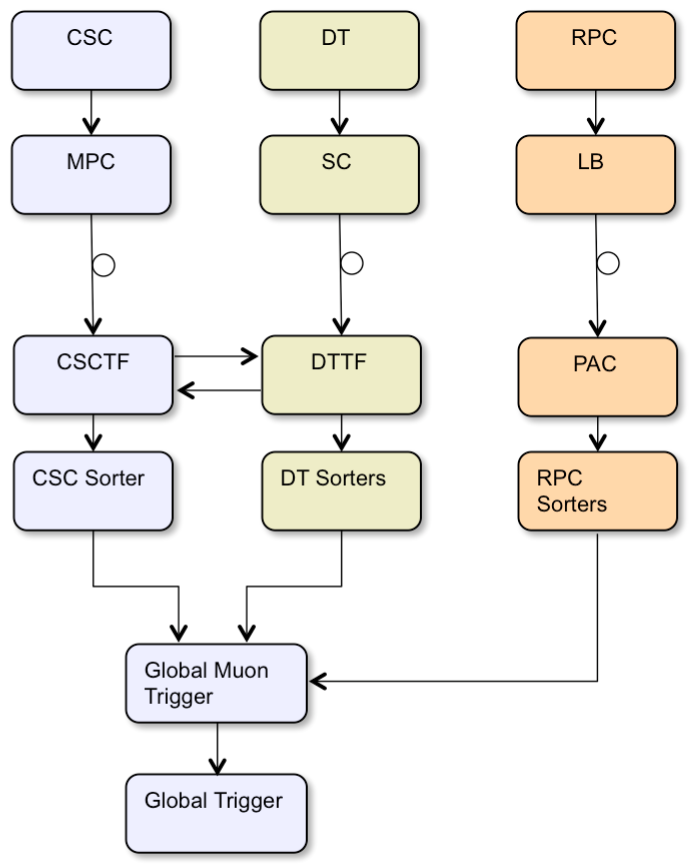
\includegraphics[width=0.48\linewidth]{figures/dataflow_current_L1_trigger.png}
	\end{center}
	\caption{Data-flow of the present L1 muon trigger. \label{fig:l1_muon_trig} }
\end{figure}

\subsection{Muon Trigger in Endcaps}

Each CSC can provide up to two local charged track (LCT) segments to the trigger logic per bunch crossing (BX, where 1 BX = 25 ns). These are formed in the trigger motherboard (TMB) combining cathode (CLCT) and anode (ALCT) segments. Present and improved logics of the algorithm which constructs LCTs are described in Section~\ref{sec:present_algo} and Section~\ref{sec:SLHC_algo}, respectively. The CLCT data contains information on the azimuthal position of the segment ($\phi$), the bend angle, and the pattern of cathode half-strips with hits in a chamber. The ALCT data contains information on the radial position from the beamline of the segment (equivalent to $\eta$), and the pattern of anode wires with hits in a chamber. The timing information from anodes is used to define the time of the combined LCT. There is one TMB per CSC, located in a crate on the periphery of the detector. The TMB sends up to two LCTs over a custom backplane to the muon port card (MPC), which is located in the same peripheral crate. One MPC can receive data from up to 9 TMBs, or equivalently, can receive up to 18 LCTs. The LCTs in a MPC are sorted by rank (see definition in MPC documentation). The best three LCTs are sent over optical fibers to the CSCTF. There are a total of sixty peripheral crates for the CSC system, each with one MPC.

The CSCTF system is partitioned into sectors, each of which corresponds to a $60^{o}$ azimuthal region of an endcap. Twelve ``sector processors'' are required for the entire endcap muon system, six per endcap. Each sector processor is a 9U VME card that is housed in a single crate. Three 1.6 Gb/s optical links from each of five MPCs are received by each sector processor, for a total of 180 optical links for the entire system. The CSCTF sectors are independent, since there is no sharing of data across boundaries of neighboring sectors, leading to slight inefficiencies.

There are several Field Programmable Gate Arrays (FPGAs) on each ``sector processor'', but the main FPGA for the track-finding algorithms is from the Xilinx Virtex-5 family. The conversion of strip and wire positions of each track segment to ($\eta, \phi$) coordinates is accomplished via a set of cascaded SRAM look-up tables (LUTs), each $512K\times16$ bits. These coordinates are then used for track-finding and momentum assignment.

The CSCTF track-finding logic consists of pairwise comparisons of track segments in different detector stations. These test for compatibility in $\phi$ and $\eta$ with a muon emanating from the collision vertex within certain tolerance windows. The comparisons are then analyzed and built into tracks consisting of possibly more than two segments from different stations. Possible duplicate (“ghost”) tracks are canceled. The track-finding logic has the ability to accept segments in different assigned bunch crossings by analyzing across a sliding time window of programmable length (nominally 2 BX) every bunch crossing. Duplicate tracks found on consecutive bunch crossings are canceled. The bunch crossing of a track is given by the second arriving track segment.

The $p_T$ of a muon candidate is calculated by using a large LUT implemented in SRAM. Information such as the track type, track $\eta$, the segment $\phi$ differences between a maximum of 3 stations, and the segment bend angle in the first measurement station are used to calculate the LUT address.

In addition to identifying muons from proton collisions, the CSCTF processors also simultaneously identifies any beam halo muons for monitoring and veto purposes by looking for trajectories approximately parallel to the beam line.

Each CSCTF sends up to three muon candidates per bunch crossing over a custom backplane to a muon sorter (MS). The MS then sorts the candidates by momentum and quality and selects the best 4 for the GMT. The CSCTF data are also sent to a DAQ card with SLINK interface which puts the trigger data into the event record.

\clearpage

\newpage
\tracinginput{sections/csc.tex}
%\section{CSC Upgrade During LS1}
\label{sec:csc}

During LS1, the outermost ring of the fourth disk of chambers of each endcap (ME4/2) will be installed. This will result in four measurement stations for muons in the region 1.25 $<$ $|\eta|$ $<$ 1.8 providing the additional redundancy needed in a high rate environment. For the L1 trigger, this coverage will improve the efficiency of the CSCTF, and improve the rate reduction since it will be more likely to have 3 or more hits used in the $p_T$ assignment logic. No additional hardware or reconfiguration of the present Level-1 trigger is required. The MPCs for the fourth
disk already are in place and the present CSCTF already has logic in place for these chambers. This redundancy will extend to the more powerful algorithms envisioned for the muon trigger upgrade as well.

The electronics for the CSC system are also under major revision. The innermost chambers of the first endcap disks (ME1/1) provide a key sagitta measurement for the L1 muon trigger in the region $1.6 < |\eta| < 2.4$. These chambers will receive new digital cathode front-end boards (DCFEB) as well as new trigger and data acquisition electronics that will significantly enhance their performance in the trigger and in offline reconstruction. The strips of the ME1/1 chambers are split into two regions at $|\eta|$ = 2.1. The bottom region $|\eta| > 2.1$ currently has strips triple-ganged in the electronics for both the trigger and readout, making it ambiguous as to which third of the chamber generated a particular hit (the ganging has every 16th strip ganged to each other, where there are 48 strips in total across a chamber layer). The ambiguity can be mitigated using measurements from the outer stations. The $p_T$ resolution using only the outer stations is quite coarse, leading to a significantly increased single muon trigger rate in the region $2.1<|\eta|<2.4$. This forward region currently generates a single muon trigger rate comparable to that of the entire
region $|\eta| < 2.1$. With the new digital front-end boards and Trigger Motherboards (TMBs), this triple-ganging will be removed, leading to much improved triggering for $2.1<|\eta|<2.4$. This should allow CMS to maintain full muon trigger coverage up to $|\eta| = 2.4$ after LS1. The recovered older electronics will be used to instrument the new ME4/2 chambers.

\begin{figure}[htb]
        \begin{center}
                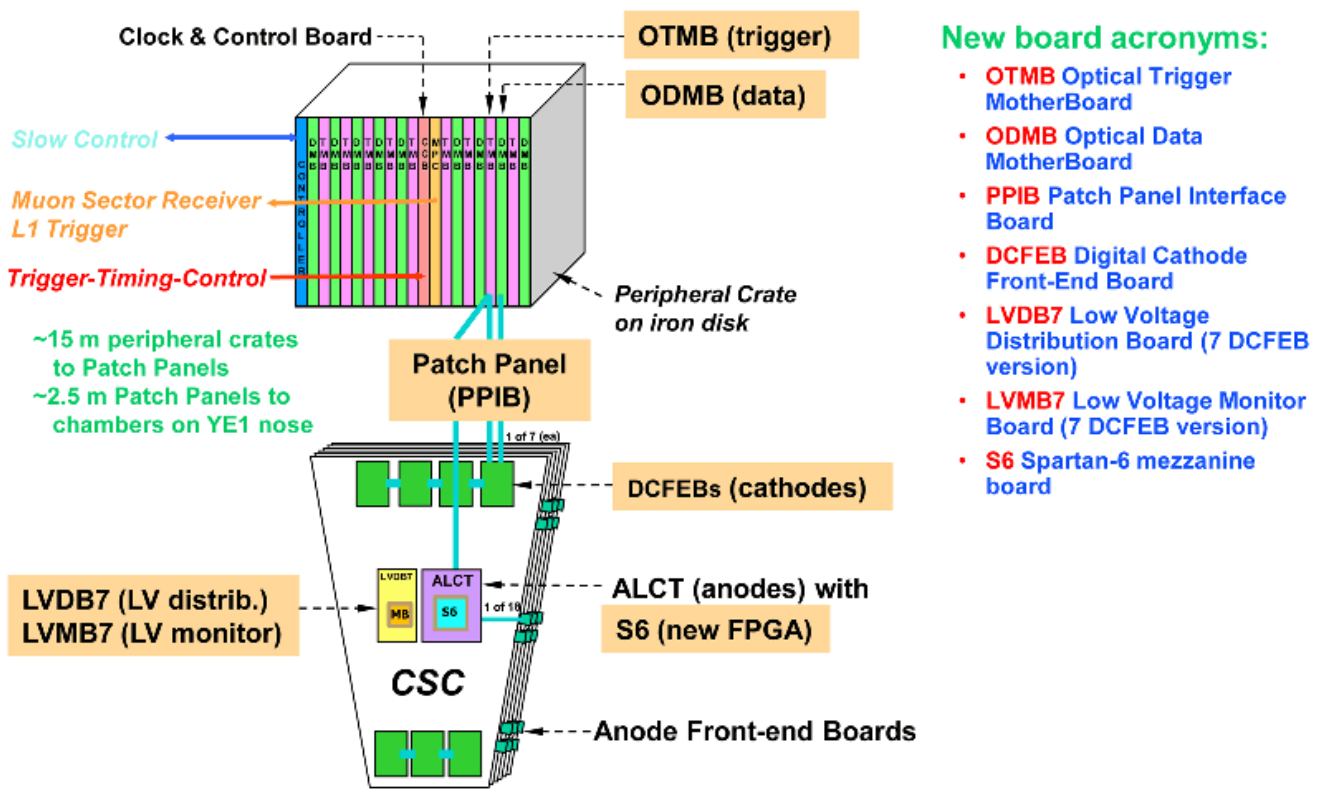
\includegraphics[width=0.90\linewidth]{figures/ME11_upgrade_overview.png}
                \caption{Schematic overview of the ME1/1 chambers upgrade.}
                \label{fig:me11_upgrade_overview}
        \end{center}
\end{figure}

\begin{figure}[htb]
        \begin{center}
                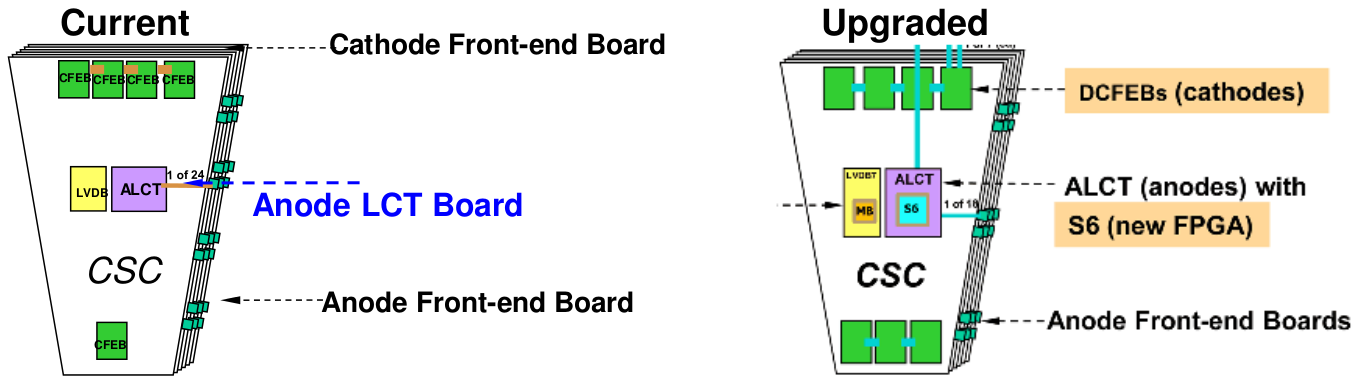
\includegraphics[width=0.90\linewidth]{figures/ME11_upgrade_electronics.png}
                \caption{Schematic overview of the ME1/1 electronics upgrade.}
                \label{fig:me11_upgrade_electronics}
        \end{center}
\end{figure}
\clearpage

\newpage
\tracinginput{sections/algorithm_2007.tex}
%\section{Present CSC Trigger Algorithm}
\label{sec:present_algo}

\subsection{ALCT Processing}

Anode wires in CSC are hardwired together at the readout end in groups of 10-15 wires in order to reduce channel count. The anode wire group (WG) signals are fed into the anode front-end boards (AFEBs), each of which contains a single 16-channel amplifier/constant-fraction discriminator chip. The output signals from the AFEBs are sent into the ALCT on-chamber board, which handles triggering and readout of the CSC anode information. Due to the various sizes of CSCs, there are 3 types of ALCT boards, handling 288, 384, and 672 anode wire group channels.

On the ALCT boards, the signals from each AFEB are first delayed by a programmable amount of time in order to perform an average time alignment of the anode signals across the chamber as well as chamber-to-chamber at a sub-bunch crossing level to about 2.2 ns precision. After the AFEB signals are received and time-aligned, then they are latched with bunch crossing frequency and fed to a FPGA (Xilinx Virtex family) mounted on a mezzanine card above the ALCT main board for pattern-finding and readout functions.

The algorithm used in the ALCT FPGA for determining muon segment position and bunch crossing is illustrated below. Since the drift time can be longer than 50 ns, the hits are first stretched by 'one-shots' to 6 BX (150 ns) length. Then, a multi-layer coincidence technique in the ALCT pattern circuitry is used to identify the bunch crossing. For each spatial pattern of anode hits, a low coincidence level, typically 2 or more layers, is used to establish timing, whereas a higher coincidence level, typically 4 layers, is used to establish the existence of a muon track. The general idea of a spatial pattern of CSC wire group hits is illustrated below in Fig.\ref{fig:anode_wire_group_hits}.

\begin{figure}[tbh]
        \begin{center}
                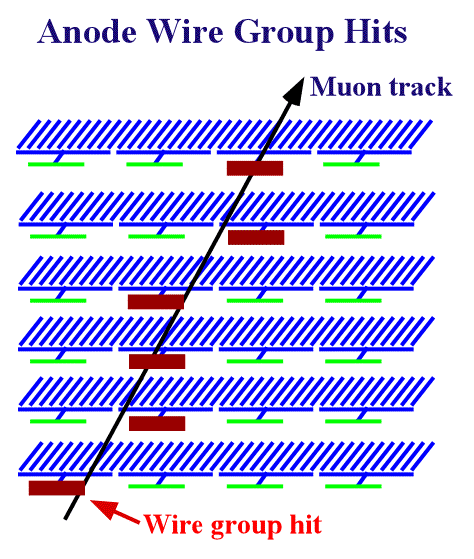
\includegraphics[width=0.48\linewidth]{figures/anode_wire_group_hits.png}
                \caption{CSC wire group patterns}
                \label{fig:anode_wire_group_hits}
        \end{center}
\end{figure}

while the general idea of the time stretching of hits, and pretrigger followed by a pattern trigger is shown in Fig.\ref{fig:anode_stretched_hits} (using an example in which one hit is actually missing due to some type of inefficiency).

\begin{figure}[tbh]
        \begin{center}
                \includegraphics[width=0.73\linewidth]{figures/anode_stretched_hits.png}
                \caption{Anode stretched hits}
                \label{fig:anode_stretched_hits}
        \end{center}
\end{figure}

Each pattern detector can detect a programmable "collision" pattern as well as a fixed "accelerator" pattern. The input data for the collision pattern detector are selected as shown below:

\begin{center}
\begin{verbatim}
...n-2 n-1 n...........Layer 1
.......n-1 n...........Layer 2
...........n...........Layer 3
...........n n+1.......Layer 4
...........n n+1 n+2...Layer 5
...........n n+1 n+2...Layer 6
\end{verbatim}
\end{center}

where n in this diagram is the key wire group number, which this particular pattern detector is searching the patterns for. The programming of the programmable collision pattern is implemented as a simple masking-out of the bits that we do not want to include in the pattern. The accelerator pattern is a vertical pattern of 6 layers all with strip n only.

Each ALCT candidate is assigned a quality equal to number of layers with hits minus 3 and passes through a ghost cancellation procedure: it is cancelled if there is another ALCT candidate at the same bunch crossing in the previous wirewith the same or better quality or in the next wire with better quality, or if there is ALCT candidate up to 4 bunch crossing clocks earlier with any quality.

In each bunch crossing two ALCTs with highest quality are sent to the TMB (Trigger MotherBoard), which requires a coincidence between anode and cathode trigger information. In the case of a Level-1 Accept signal from the Global Trigger (distributed via the TTC system to the CCB in each peripheral crate), ALCT data are sequentially transmitted to the Trigger Mother Board and hence to the DAQ Motherboard. These data frames include a few words of ALCT trigger data and a much larger amount of ALCT raw hit data consisting of a time sequence of raw CSC anode wire-group hits that have been stored at the 40 MHz bunch crossing frequence by the ALCT2001. Typically 8 to 16 bunch crossings are read out for each wire group. FIFO data can also be read out much more slowly through VME access via the TMB board using a JTAG electrical interface to the ALCT, if necessary.

For self-monitoring and also for powering and controlling the AFEB cards, the ALCT contains a Slow Control section that supplies power to the AFEBs, controls AFEB thresholds, provides and controls the amplitude of test pulses to the AFEBs, and reads back power supply voltages and currents, as well as on-board temperature. 

\newpage
\subsection{Software Emulation of ALCT Processing}

ALCT processing includes the following five steps:

\begin{itemize}
    \item Pulse extension;
    \item Pretrigger;
    \item Trigger;
    \item Ghost cancellation;
    \item ALCT construction.
\end{itemize}

\subsubsection{Pulse Extension}

Sofware emulation provides information about all wire signals in DAQ readout window (16 BXs). A search for these signals is performed in a loop over all wire groups, all layers, and all 16 BXs; found signals are stretched over 6 BXs (see Fig.~\ref{fig:alct_pulse_extension}).

\begin{figure}[tbh]
        \begin{center}
                \includegraphics[width=0.9\linewidth]{figures/stretched_hits_alct.pdf}
                \caption{Illustration of ALCT pulse extension for one specific wire group.}
                \label{fig:alct_pulse_extension}
        \end{center}
\end{figure}

\subsubsection{Pretrigger}

After all available wire signals are stretched, a search for ALCT pretriggers is performed in all wire groups and all BXs. For any given wire group and BX, we count the number of layers with hits within the pattern mask shown on Fig.~\ref{fig:alct_pretrigger}, and if this number is greater than or equal to three, then we say that a pretrigger occured in this wire group and BX. The search for next ALCT pretrigger starts 6 BXs later.

\begin{figure}[tbh]
        \begin{center}
                \includegraphics[width=0.45\linewidth]{figures/alct_pretrigger.pdf}
                \caption{ALCT pattern mask for pretriggering and triggering.}
                \label{fig:alct_pretrigger}
        \end{center}
\end{figure}

\subsubsection{Trigger}

After all ALCT pretriggers are found, for each pretrigger in BX = B we check for a trigger in BX = B+2. For any given wire group and BX = B+2, we count the number of layers with hits within the same pattern mask used for pretriggering, and if this number is greater than or equal to four, we say that a pretrigger occured in this wire group and BX, and assign it a quality Q = number of layers with hits-3. If in some wire group more than one trigger occured, we report only the one with the highest quality. If there are two triggers with the same quality, report the earlier one.

\subsubsection{Ghost Cancellation}

Not all triggers found in the previous step are used to construct ALCTs: before that all of them pass through so called ghost cancellation procedure.

A trigger in wire group = N and BX = B is cancelled if there is a trigger in wire group = N-1:
\begin{itemize}
    \item either in the same BX = B and with better or equal quality;
    \item or to 4 BXs earlier, with any quality.
\end{itemize}

In addition, a trigger in wire group = N and BX = B is cancelled if there is a trigger in wire group = N+1:
\begin{itemize}
    \item either in the same BX = B and with better quality;
    \item or to 4 BXs earlier, with any quality.
\end{itemize}

\subsubsection{ALCT Construction}

Construct ALCTs from triggers survived after the ghost cancellation procedure: encode quality, WG, BX (defined by pretrigger BX). In every BX choose best two ALCTs: two ALCTs with the highest quality. If we need to choose one ALCT from two ALCTs with the same quality: choose the one with larger wire group.

\newpage
\subsection{CLCT Processing}

[We need a good picture illustrating CLCT processing process like in the case of ALCT one]

A muon passing through a CSC chamber will produce distinctive patterns of half-strip
hits in the six-layer endcap muon CSC chambers. By identifying these patterns, the CSC Local
Trigger provides high rejection power against backgrounds. The largest background source,
neutron-induced gamma ray conversions, are generally low in energy, and produce mostly single-
layer or short multi-layer hits. Other backgrounds, such as low-momentum muons or punch-
through particles often do not point well enough to the primary interaction region to be considered
high-momentum muon candidates.

\begin{figure}[tbh]
        \begin{center}
                \includegraphics[width=0.73\linewidth]{figures/CLCT_block_diagram.png}
                \caption{CLCT block diagram}
                \label{fig:clct_block_diagram}
        \end{center}
\end{figure}

[Technical description from TMB manual below]

For each of 160 key half-strips consider the 42 neighboring half-strips (i.e. on key 5 use the following half-strips):

\begin{figure}[tbh]
        \begin{center}
                \includegraphics[width=0.48\linewidth]{figures/160_key_half_strips.png}
                \caption{160 key half-strips}
                \label{fig:160_key_half_strips}
        \end{center}
\end{figure}

For each of 160 key half-strips, count layers with hits matching the 9 pattern templates:

\begin{figure}[tbh]
        \begin{center}
                \includegraphics[width=0.98\linewidth]{figures/CLCT_patterns.png}
                \caption{CLCT patterns}
                \label{fig:clct_patterns}
        \end{center}
\end{figure}

Pattern ID=1 is a layer-OR trigger, Pattern ID=0 is no-pattern-found. Result for each of 160 keys is a list of 9 pattern-ID numbers (pid) [2 to A] and corresponding
number of layers [0 to 6] with matching hits (nhits). Find the best 1-of-9 pattern ID numbers for each key by comparing nhits. Ignore bend direction: left and right bends have equal priority (bit 0 of pid implies bend direction).
If two pattern IDs have the same nhits, take the higher pattern ID. A key with no matching hits, would always return pid=A and nhits=0.
Pre-trigger if any 1-of-160 keys have nhits $\geq$ hit\_thresh\_pretrig and pid $\geq$ pid\_thresh\_pretrig.

Construct 7-bit pattern quality pat[7:0] for sorting where pat[7:5]=nhits[2:0], pat[4:0]=pid[3:0]. Ignore the bend direction bit (pid[0]), left and right bends have equal priority. 
Store pat[7:0] for 160 keys for use later to find 2nd CLCT.
Find the best key out 1-of-160 keys by sorting on the 6-bit number pat[7:1]. Store 1st CLCT info: key, pattern ID, and number of hits.
For empty events, key=0, pid=A and nhits=0. If clct\_blanking=1, then key=pid=hits=0.

Mark keys near 1st CLCT as busy from 1st key-nspan to 1st key+pspan.
If clct\_sep\_src=1, pspan and nspan are set equal to clct\_sep\_vme, typically 10 half-strips.
If clct\_sep\_src=0, pspan and nspan are read from RAM and depend on the pattern ID number, this allows two less bending tracks to be closer than more bending tracks.

Find the best key out of 1-of-160 keys by sorting on the 6-bit number pat[7:1]: skip busy keys, if two keys have the same pat[7:1] take the lower key.
Store the same information for the 2nd CLCT as for the 1st one.

Wait for CSC drifting (drift delay of 2BXs) and perform matching to ALCTs.

\newpage
\subsection{Software Emulation of CLCT Processing}

CLCT processing includes the following four steps:

\begin{itemize}
    \item Pulse extension;
    \item Pretrigger;
    \item Trigger;
    \item CLCT construction and CLCT dead time.
\end{itemize}

In contrast to ALCT processing, where all steps are independent and performed one after another for all 16 BXs, during CLCT processing last three steps repeated in one global loop over BXs.

\subsubsection{Pulse Extension}

Sofware emulation provides information about all half-strip signals in DAQ readout window (16 BXs). A search for these signals is performed in a loop over all half-strips, all layers, and all 16 BXs; found signals are stretched over 6 BXs (see Fig.~\ref{fig:clct_pulse_extension}).

\begin{figure}[tbh]
        \begin{center}
                \includegraphics[width=0.9\linewidth]{figures/stretched_hits_clct.pdf}
                \caption{Illustration of ALCT pulse extension for one specific half-strip.}
                \label{fig:clct_pulse_extension}
        \end{center}
\end{figure}

\subsubsection{Pretrigger}

After all available half-strip signals are stretched, start a global loop over all BXs from BX = 0 and search for CLCT pretriggers in all half-strips. For any given BX and half-strip, count the number of layers with hits within the patterns shown on Fig.~\ref{fig:clct_pretrigger}, and if this number is greater than or equal to three, then we say that a pretrigger occured in this BX and this half-strip. This pretrigger is only accepted if its pattern id $\geq$ 2. If there were no CLCTs found in some BX = B, proceed to BX = B+1 and continue searching for pretriggers. If there are some CLCTs found in the current BX, proceed to next step.

\begin{figure}[tbh]
        \begin{center}
                \includegraphics[width=0.48\linewidth]{figures/clct_pattern_01.pdf}
                \includegraphics[width=0.48\linewidth]{figures/clct_pattern_10.pdf}\\
                \includegraphics[width=0.48\linewidth]{figures/clct_pattern_02.pdf}
                \includegraphics[width=0.48\linewidth]{figures/clct_pattern_03.pdf}\\
                \includegraphics[width=0.48\linewidth]{figures/clct_pattern_04.pdf}
                \includegraphics[width=0.48\linewidth]{figures/clct_pattern_05.pdf}\\
                \includegraphics[width=0.48\linewidth]{figures/clct_pattern_06.pdf}
                \includegraphics[width=0.48\linewidth]{figures/clct_pattern_07.pdf}\\
                \includegraphics[width=0.48\linewidth]{figures/clct_pattern_08.pdf}
                \includegraphics[width=0.48\linewidth]{figures/clct_pattern_09.pdf}
                \caption{CLCT patterns for pretriggering and triggering.}
                \label{fig:clct_pretrigger}
        \end{center}
\end{figure}

\subsubsection{Trigger}

As soon as a BX = B with CLCT pretrigger(s) is found, search for triggers in BX = B+2. For each half-strip, count the number of layers with hits within the same patterns used for pretriggering, and if this number is greater than or equal to four, we say that a trigger occured in this half-strip and BX, and remember:
\begin{itemize}
    \item pattern id with the highest number of hit layers (if there are two pattern ids with the same number of hit layers, choose smaller pattern id);
    \item number of hit layers in this pattern id.
\end{itemize}

Proceed to next step.

\subsubsection{CLCT Construction and CLCT Dead Time}

In a BX with CLCT triggers, find up to two best triggers to be used in CLCT construction.

Find the best trigger:
\begin{itemize}
    \item Find trigger with the highest number of hit layers;
    \item If there are two triggers with the same number of hit layers: choose the one with higher pattern id;
    \item If there are two triggers with the same number of hit layers and the same pattern id: choose the one with smaller half-strip.
\end{itemize}

Mark zone of 20 half-strips around the best trigger as used and find the second best trigger among not used half-strips.

Construct up to two best CLCTs from found best triggers: encode quality, pattern, bending direction, half-strip, cfeb, BX (defined by pretrigger BX).

After CLCT construction, keep CLCT "dead": continue the loop over all BXs until there is a BX with no triggers. When such a BX is found go back to pretriggering step.

\newpage
\subsection{CLCT and ALCT Correlation}

The Trigger Motherboard (TMB) portion of the CLCT/TMB card receives up to two
anode stubs from the ALCT board and two cathode stubs from the CLCT portion of the CLCT/
TMB card. The functions of the TMB circuitry are:

\begin{itemize}
	\item Bunch crossing alignment of the anode and cathode tags.
	\item Correlation of the Anode and Cathode LCT words and construction of two combined LCTs.
	\item Transmission of LCT data to the Muon Port Card (MPC) for triggering, and transmission of DAQ data to the DAQ Motherboard (DAQMB).
\end{itemize}

Incoming anode and cathode LCTs are not aligned in time. Anode LCTs are created
faster than cathode LCTs because of the slow development of the cathode preamp signal, and
because processing inside the ALCT card is faster than processing inside the CLCT logic. The
TMB contains input pipeline logic in order to delay anode LCTs for a programmable number of
bunch crossings up to 10.

The anode and cathode LCTs are matched according to the more precise ALCT bunch
crossing number (BXN). The Cathode LCT BXN can differ by at most $\pm$1 bunch crossing. For each
of the selected muons the TMB outputs a 2-bit bunch crossing match word as shown in
table below. These may be used by later boards in the trigger chain if additional quality information
is needed. They also allow the analysis of the bunch crossing matching in the TMB, since a large
number of bad matches could be an indication of a timing alignment problem.

The ideal case for a high-momentum muon is one anode and one cathode LCT pattern.
However, other cases may occur, which are distinguished by a 2-bit “STA” (Status type A) code:

\begin{itemize}
	\item The TMB may receive one or two anode LCTs and zero cathode LCT patterns. This
happens, for example, for very low-momentum muons. Although the non-zero data is
forwarded to the MPC, this case is flagged by STA=1, as is the similar case of one or two
cathode LCT and zero anode LCT patterns.
	\item If the TMB receives two anode LCTs and one cathode LCT, the TMB outputs two LCTs,
by copying the Cathode LCT bits into both muons. These, and the similar case of two
cathode LCTs and one anode LCT, are flagged by STA=2.
	\item If there are two anode LCTs and two cathode LCTs in one chamber, they are matched
according to their pattern numbers: the largest ALCT and CLCT pattern numbers are
paired, and the second largest ALCT and CLCT pattern numbers are paired. These, and
the ideal case of a single match, are flagged by STA=3.
\end{itemize}

TMBs maintain a local Bunch Crossing Number (BXN) using signals from the Clock
and Control Board. The internal BXN is compared to the BXN received from the ALCT module,
and the Sync Error bit is set if a mismatch is detected.

The TMB sends up to two anode LCT and two cathode LCT patterns for one CSC
chamber to the MPC every 25 ns.

\newpage
\subsection{Software Emulation of CLCT and ALCT Correlation}

Every BX OTMB receives up to 2 CLCTs and up to two ALCTs from CLCT and ALCT processors, Fig.~\ref{fig:clcts_alcts} shows an example which will be used throughout the subsection.

\begin{figure}[tbh]
        \begin{center}
                \includegraphics[width=0.7\linewidth]{figures/clcts_alcts.pdf}
                \caption{Example of CLCTs and ALCTs received by OTMB.}
                \label{fig:clcts_alcts}
        \end{center}
\end{figure}

There are two approaches to CLCT and ALCT correlation: CLCT-centric and ALCT-centric. We will introduce the former below and discuss the latter later among OTMB level improvements.

CLCT-centric CLCT and ALCT correlation (see Fig.~\ref{fig:clct_alcts}):
\begin{itemize}
    \item Loop over CLCT BXs from BX = 0 to BX = 15
    \item For CLCT BX = B with at least one valid CLCT:
    \begin{itemize}
        \item Loop over ALCT BXs from BX = B-3 to BX = B+3
        \item Find the first ALCT BX in the matching window with at least one valid ALCT and not marked as used before
        \begin{itemize}
            \item Correlate CLCTs and ALCTs in matching ALCT and CLCT BXs
            \item Mark ALCT BX as used
            \item Proceed to next CLCT BX
        \end{itemize}
    \end{itemize}
\end{itemize}

\begin{figure}[tbh]
        \begin{center}
                \includegraphics[width=0.7\linewidth]{figures/clct_alcts.pdf}
                \caption{CLCT-centric CLCT and ALCT correlation.}
                \label{fig:clct_alcts}
        \end{center}
\end{figure}

The results of such a correlation are shown on Fig.~\ref{fig:clct_alcts_end}.

\begin{figure}[tbh]
        \begin{center}
                \includegraphics[width=0.7\linewidth]{figures/clct_alcts_end.pdf}
                \caption{Result of CLCT-centric CLCT and ALCT correlation.}
                \label{fig:clct_alcts_end}
        \end{center}
\end{figure}

By default, LCTs are constructed only from valid CLCTs and ALCTs, but we may optionally allow construction of ALCT-less or CLCT-less LCTs.

If there are no ALCT BXs with at least one valid ALCT in the watching window and ALCT-less LCTs are allowed, construct LCTs from valid CLCTs in the current CLCT BX (see example on Fig.~\ref{fig:clct_alcts_alctless} with results on Fig.~\ref{fig:clct_alcts_alctless_end}).

\begin{figure}[tbh]
        \begin{center}
                \includegraphics[width=0.7\linewidth]{figures/clct_alcts_alctless.pdf}
                \caption{Example of construction of ALCT-less LCTs.}
                \label{fig:clct_alcts_alctless}
        \end{center}
\end{figure}

\begin{figure}[tbh]
        \begin{center}
                \includegraphics[width=0.7\linewidth]{figures/clct_alcts_alctless_end.pdf}
                \caption{Results of construction of ALCT-less LCTs.}
                \label{fig:clct_alcts_alctless_end}
        \end{center}
\end{figure}

If there are no valid CLCTs in the current CLCT BX and CLCT-less LCTs are allowed (see example on Fig.~\ref{fig:clct_alcts_clctless} with results on Fig.~\ref{fig:clct_alcts_clctless_end}):
\begin{itemize}
    \item Find first ALCT BX in the matching window with at least one valid ALCT and not marked as used before;
    \item Construct LCTs from valid ALCTs in that ALCT BX.
\end{itemize}

\begin{figure}[tbh]
        \begin{center}
                \includegraphics[width=0.7\linewidth]{figures/clct_alcts_clctless.pdf}
                \caption{Example of construction of CLCT-less LCTs.}
                \label{fig:clct_alcts_clctless}
        \end{center}
\end{figure}

\begin{figure}[tbh]
        \begin{center}
                \includegraphics[width=0.7\linewidth]{figures/clct_alcts_clctless_end.pdf}
                \caption{Results of construction of CLCT-less LCTs.}
                \label{fig:clct_alcts_clctless_end}
        \end{center}
\end{figure}

When we use default behavior, where LCTs are constructed only from valid CLCTs and ALCTs, the ideal case is when in matching BXs number of valid CLCTs is equal to number of valid ALCTs (see top two examples on Fig.~\ref{fig:clct_alct_corr}).

\begin{figure}[tbh]
        \begin{center}
                \includegraphics[width=0.7\linewidth]{figures/clct_alct_corr.pdf}
                \caption{Construction of LCTs.}
                \label{fig:clct_alct_corr}
        \end{center}
\end{figure}

But when, for example, there is only one valid CLCT and two valid ALCTs, we make the second valid CLCT from the first, analogously, when there are two valid CLCTs and only one valid ALCT (see bottom two examples on Fig.~\ref{fig:clct_alct_corr}).
\clearpage

\newpage
\tracinginput{sections/algorithm_SLHC.tex}
%\section{Improved CSC Trigger Algorithm for High Luminosity Running}
\label{sec:SLHC_algo}

\subsection{Separate finding of CLCTs in ME1/a and ME/1b}

 In the old TMB f/w, the 16 ganged strip channels from ME1/a are appended to the 64 ME/1b strip channels and the reconstruction of CLCTs is performend as if it's a single regular chamber with 80 channels (is there any treatment of the boundary, so that ME1/a strips are not combined with ME1/b strips?). The two rather separate and distinctive areas combined and treated like one uniform unit with the maximum of two CLCT stubs on the output.

With unganged ME1/a and higher pile-up such a simple approach becomes increaingly unnatural and ineffective. The ME1/a would have x3 more channels now, so it would deserve to be treated like a seperate chamber even more. And chances to get multiple stubs are increasing with higher luminosity, especially so in ME1/a. With multiple stubs, the stubs in ME1/a would start directly competing with those in ME1/b.

With a larger size FPGA, it would be beneficial to treat ME1/a and ME1/b as two separate chambers for the purpose of CLCT reconstruction, with each area having their own limit on the maximum of 2 CLCTs. Thus, the whole ME1/1 would be able to have maximum 4 CLCTs available for matching with ALCTs. It's important to keep more 2D stubs available so that at the stage of matching we can reduce the number of stubs following some better tuned criteria.

Finally, in the case if we would allow to read out the 2D CLCT stubs without an ALCT match, and we cannot read out more then 2 of them per BX per ME1/1, we can device a selection criteria when comparing stubs from ME1/a and 1/b as follows: e.g., if quality of an ME1b stub is the same or less by one then that of an MEr 1a stub, prefer the ME1b one. 

\subsection{Localizing the TMB dead time }

 The main source of the old TMB inefficiency in high pile-up is the dead time which happens for the whole ME1/1 chamber after there was a triggering CLCT. The TMB's state-machine freezes whole TMB for several BXs after a CLCT trigger while number of coincidence layers stays over the trigger threshold. If anywhere in a chamber there was an CLCT from PU a few BX earlier before a signal muon, it would be impossible to trigger on the signal.

While it's clear that with the comparator information which we recieve in TMB, it's not really possible to distinguish close in time signals in the same strip, there seem to be no apparent reason, other then the complexity of the algorithm, for this dead time to be present in strips that had no trigger.

Thus, the algorithm approach to deal with this issue for the upgrade could be as follows:
\begin{itemize}
    \item when a CLCT trigger happens, mark as busy only those strips within either a fixed dead time zone around CLCT (8 half-strips, see "useDeadTimeZoning" parameter in Sec.~\ref{sec:CLCT_conf}) or within the dead time zone, the width of which depends on the CLCT pattern (from 11 half-strips for the most bent patterns to 3 half-strips for the straightest one, see "useDynamicStateMachineZone" parameter in Sec.~\ref{sec:CLCT_conf}), and also mark the signal half-strip that specifies the triggered CLCT
    \item during the following bunch-crossings, check if the number of coincidence layers drops under the trigger threshold for the signal half-strip
    \begin{itemize}
	\item if it does, remove the "busy" mark from the corresponding strips 
    \end{itemize}
    \item if strips are marked as busy in a BX, they are excluded from pattern recognition 
\end{itemize}

\subsection{Restriction of CLCT pattern bend }

 The current set of CLCT patterns (e.g., see p5 of TMB2005\_spec\_v4p55) is largely geared towards low pt tracks. For tracks with pt>10, only the straighest and the next one bent patterns are significant. The restriction on allowed pattern bending would significantly help with many issues including multiplicity \& rate, ghosting, dead-time and corresponding loss of the efficiency (see "clctPidThreshPretrig" parameter in Sec.~\ref{sec:CLCT_conf}). Positive effect of it would increase with increasing luminosity. However, it would also somewhat reduce the efficiency because of not so good pt-threshold resolution from fairly narrow (11cm) CSC chambers, especially for medium to lower pt muons.

TODO: need a plot showing the efficiency vs pt for a simtrack to have a matching reconstricted CLCT stub for different maximum thresholds for the bend. GEMs could be helpful for improving the effectivenes and the efficiency of the bend restriction. 

\subsection{Improving CLCT timing }

 Currently, the BX time of a CLCT stub is defined as the BX of its pretrigger. Or, in other words, it's first BX when at least three layers fit one of the CLCT patterns. Note that an attempt to latch a trigger pattern is performed after the number of BX after the pretrigger defined by the clctDriftDelay parameter (=2BX). And also note that a CLCT pattern during the pretrigger could be different then the one that happen to match during the trigger.

With higher luminosity there are increasingly larger chances for some strips in some of the layers to be hit by earlier background hit. And that has chances to affect the time when a pretrigger might be detected. A more robust solution would be to define stub's time using the times of its strips, where stub's strips are defined as strips that were matched within a CLCT pattern during the trigger. As for a specific procedure, a median time over those strips' times or some sort of a truncated average could be used (see "clctUseCorrectedBx" parameter in Sec.~\ref{sec:CLCT_conf}, analogously for "alctUseCorrectedBx" parameter in Sec.~\ref{sec:ALCT_conf}).

\subsection{ALCT Handling }

 It should be possible to improve the efficiency, rate and timing precision of ALCT stubs by, e.g.
\begin{itemize}
    \item tuning of the ghost cancellation logic (ALCTs in neighboring wiregroups, see "alctGhostCancellationBxDepth" and "alctGhostCancellationSideQuality" parameters in Sec.~\ref{sec:ALCT_conf}) and removing pre-trigger deadtime (see "alctPretrigDeadtime" parameter in Sec.~\ref{sec:ALCT_conf});
    \item using more narrow ALCT pattern in ring 1 chambers (see "alctNarrowMaskForR1" parameter in Sec.~\ref{sec:ALCT_conf});
    \item using more precise algorithm (e.g., running median or truncated average) for BX assignment (see "alctUseCorrectedBx"  parameter in Sec.~\ref{sec:ALCT_conf}).
\end{itemize}

However, here we would only like to focus on how the ALCT stubs would be used by TMB.

ALCTs are reconstructed from the signals in layers of anode wires which are ganged into wiregroups and are continuously covering the whole ME1/1 chamber. Most of the wiregroups can only physically cross only strips either in ME1/a or only in ME1/b. A complication specific to ME1/1 is that wires here are not perpendicular to strips, but are slanted at 29 degrees from the straight angle. Thus, some wiregroups are crossing the border between ME1/a and ME1/b. If signal is detercted in such a wiregroup, there is an ambiguity about which part of ME1/1 it might belong to.

For the ALCTs received by TMB we propose to split the incoming stubs into two parts, ME1/a and ME1/b, that would be used further for LCT matching separately in ME1/a and ME1/b. 

\subsection{Narrowing the matching time window }

 The current TMB uses a rather wide time matching window (7BX) that is centered on a CLCT's BX, and is used to look for an ALCT match within it. A wide matching window is not good in high pileup, as propability of incorrect matching with background 2D stubs is higher, resulting in inefficiency.

For the SLHC, we can probably assume that the system is well timed and that we can use the narrowest reasonable matching window of 3BX wide (see "matchTrigWindowSize" parameter in Sec.~\ref{sec:TMB_conf}). 

\subsection{Modification of the stub timing logic in matching }

 In the old TMB algorithm, the stub timing logic works during the 2D stubs matching as follows:
\begin{itemize}
    \item CLCT-centric approach: CLCTs and their BX are taken as reference points, while ALCTs are waiting in a queue
    \item for a BX with CLCTs we look for a first BX in the matching window that has ALCTs
    \item after matching is dome in this BX, the ALCTs from there are taken off the queue, and cannot be matched with any later CLCT (see "tmbDropUsedClcts" and "matchEarliestClctME11Only" parameters in Sec.~\ref{sec:TMB_conf})
\end{itemize}

The main issues with this approach at high luminosity is that when there is an ALCT from a good signal muon, early CLCTs from background might steal it and form wrong match, and this correct ALCT then would not be available anymore for matching with a later correct CLCT.

Proposal to improve the situation:
\begin{itemize}
    \item ALCT-centric approach: ALCTs and their BXs are taken as reference points, while reconstructed CLCTs are waiting in a matching window-wide queue (see "clctToAlct" parameter in Sec.~\ref{sec:TMB_conf})
    \begin{itemize}
        \item ALCT's BX and the middle BX in the matching window-wide queue are expected to be synchronized 
    \end{itemize}
    \item for an ALCT's BX we look for CLCTs within the queue in the order of arrival try to find maximum 2 LCT matches as follows (see "tmbCrossBxAlgorithm" parameter in Sec.~\ref{sec:TMB_conf}):
    \begin{itemize}
        \item first look for CLCTs in the same BX 2) if we didn't get 2 LCT matches yet, look for CLCTs in BX-1
        \item if we didn't get 2 LCT matches yet, look for CLCTs in BX+1
        \item etc... depending on how wide the matching window is 
    \end{itemize}
    \item can optionally either remove CLCTs from the queue after there was an LCT match, or can keep them for reuse possibilities to be matched with later ALCTs (see "tmbDropUsedClcts" parameter in Sec.~\ref{sec:TMB_conf})
    \item NOTE: all this is supposed to be done separately in ME1a and in ME1b 
\end{itemize}

\subsection{Selecting up to two the best LCTs per ME1/1}

With the backplane limitations, we can read out only up to two trigger stubs per BX from the whole ME1/1.

Since ME1/a and ME1/b now can each have up to two stubs, we need an extra step of selecting the best two ME1/1 stubs out of possible 4. If ME1/a + ME1/b has more then two LCTs:
\begin{itemize}
    \item The simplest solution:
    \begin{itemize}
	\item drop the highest eta ones until we have just two. 
    \end{itemize}
    \item Possible improvement:
    \begin{itemize}
        \item rank stubs by special quality value which is the same as stub quality for ME1/b and is stub quality-1 for ME1/a stubs
        \item if special quality is the same, rank by eta 
    \end{itemize}
\end{itemize}

\newpage
\subsection{Sofware Emulation of ALCT Level Improvements}

\subsubsection{Tuning of Ghost Cancellation Procedure}

\textcolor{red}{Current} ghost cancellation:
\begin{itemize}
    \item Loop over wire groups:
    \begin{itemize}
        \item Consider WG = N
        \item Cancel trigger in this wire group if there is trigger in WG = N-1 and:
        \begin{itemize}
            \item with the same BX and with \textcolor{red}{better or equal} quality
            \item up to \textcolor{red}{4} BXs earlier, with \textcolor{red}{any} quality
        \end{itemize}
        \item Cancel trigger in this wire group if there is trigger in WG = N+1 and:
        \begin{itemize}
            \item with the same BX and with \textcolor{red}{better} quality
            \item up to \textcolor{red}{4} BXs earlier, with \textcolor{red}{any} quality
        \end{itemize}
    \end{itemize}
\end{itemize}
\textcolor{blue}{New} ghost cancellation:
\begin{itemize}
    \item Loop over wire groups:
    \begin{itemize}
        \item Consider WG = N
        \item Cancel trigger in this wire group if there is trigger in WG = N-1 and:
        \begin{itemize}
            \item with the same BX and with \textcolor{blue}{better} quality
            \item up to \textcolor{blue}{1} BX earlier, with \textcolor{blue}{better} quality
        \end{itemize}
        \item Cancel trigger in this wire group if there is trigger in WG = N+1 and:
        \begin{itemize}
            \item with the same BX and with \textcolor{blue}{better or equal} quality
            \item up to \textcolor{blue}{1} BX earlier, with \textcolor{blue}{better and equal} quality
        \end{itemize}
    \end{itemize}
\end{itemize}

The following modifications in configuration are related to this improvement:
\begin{itemize}
    \item alctGhostCancellationBxDepth: 4BX to 1BX
    \item alctGhostCancellationSideQuality: False to True
\end{itemize}

\subsubsection{Narrow ALCT Pattern Mask}

Use more narrow ALCT pattern mask for stations in Ring 1 (see Fig.~\ref{fig:narrow_alct_pattern_mask}).

\begin{figure}[tbh]
        \begin{center}
                \includegraphics[width=0.49\linewidth]{figures/alct_pretrigger.pdf}\\
                \includegraphics[width=0.49\linewidth]{figures/alct_pretrigger_r1.pdf}
                \caption{Top: default ALCT pattern mask, bottom: narrow ALCT pattern mask.}
                \label{fig:narrow_alct_pattern_mask}
        \end{center}
\end{figure}

The following modifications in configuration are related to this improvement:
\begin{itemize}
    \item alctNarrowMaskForR1: False to True
\end{itemize}

\subsubsection{Reduced ALCT Dead Time}

Currently, if there is pretrigger in BX = B (see Fig.~\ref{fig:alct_deadtime}):
\begin{itemize}
    \item Check for trigger in BX = B + drift time = B+2
    \item Search for next pretrigger starting from BX = B + drift time + extra deadtime = B+6
\end{itemize}

Suggested improvement: decrease extra deadtime from 4 BX to 0 BX.

\begin{figure}[tbh]
        \begin{center}
                \includegraphics[width=0.98\linewidth]{figures/stretched_hits_alct_deadtime.pdf}
                \caption{Top: Dead Time between ALCT pretriggers.}
                \label{fig:alct_deadtime}
        \end{center}
\end{figure}

The following modifications in configuration are related to this improvement:
\begin{itemize}
    \item alctPretrigDeadtime: 4BX to 0BX
\end{itemize}

\newpage
\subsection{Sofware Emulation of CLCT Level Improvements}

\subsubsection{Localizing Dead Zone}

\textcolor{red}{Current implementation of dead time}:
\begin{itemize}
    \item After constructing up to two CLCTs, \textcolor{red}{continue the loop over all BXs until there is a BX with no triggers}
    \\...
    \item In the BX with trigger, construct up to two CLCTs from two best triggers \textcolor{red}{in all half-strips}
    
\end{itemize}
\textcolor{blue}{New implementation of dead time}:
\begin{itemize}
    \item After constructing up to two CLCTs, \textcolor{blue}{mark 16 half-strips around half-strips of these CLCTs as busy while number of hit layers in half-strips of these CLCTs $\geq$ 4}
    \item \textcolor{blue}{After trigger in BX = B, keep searching for pretrigger in strating from BX = B+1}
    \\...
    \item In the BX with trigger, construct up to two CLCTs from two best triggers \textcolor{blue}{in half-strips}
    \begin{itemize}
        \item \textcolor{blue}{within 5 half-strips from pretrigger half-strips}
        \item \textcolor{blue}{which are not marked as busy from previous trigger}
    \end{itemize}
\end{itemize}

The following modifications in configuration are related to this improvement:
\begin{itemize}
    \item useDeadTimeZoning: False to True
\end{itemize}

\subsubsection{Dynamic Dead Zone Width}

\textcolor{red}{Fixed dead time zone}:
\begin{itemize}
    \item After constructing up to two CLCTs, mark \textcolor{red}{16} half-strips around half-strips of these CLCTs as busy while number of hit layers in half-strips of these CLCTs $\geq$ 4
\end{itemize}
\textcolor{blue}{Dynamic dead time zone}:
\begin{itemize}
    \item After constructing up to two CLCTs, mark \textcolor{blue}{K(pid)} half-strips around half-strips of these CLCTs as busy while number of hit layers in half-strips of these CLCTs $\geq$ 4
\end{itemize}
\vskip3mm
K(pid) --- function of pattern id:
\begin{itemize}
    \item K(1,2,3) = 22 half-strips
    \item K(4,5) = 18 half-strips
    \item K(6,7) = 14 half-strips
    \item K(8,9) = 10 half-strips
    \item K(10) = 6 halt-strips
\end{itemize}

The following modifications in configuration are related to this improvement:
\begin{itemize}
    \item useDynamicStateMachineZone: False to True
\end{itemize}

\newpage

\subsubsection{Minimal Pattern ID for Pretriggering}

\textcolor{red}{Current CLCT pretrigger}:
\begin{itemize}
    \item Loop over all BXs (starting from BX = 0) and all half-strips:
    \begin{itemize}
        \item Count number of layers with hits in the following patterns
        \item If this number $\geq$ 3: pretrigger occurs
        \item Accept this pretrigger if its pattern id $\geq$ \textcolor{red}{2}
    \end{itemize}
\end{itemize}
\textcolor{blue}{New CLCT pretrigger}:
\begin{itemize}
    \item Loop over all BXs (starting from BX = 0) and all half-strips:
    \begin{itemize}
        \item Count number of layers with hits in the following patterns
        \item If this number $\geq$ 3: pretrigger occurs
        \item Accept this pretrigger if its pattern id $\geq$ \textcolor{blue}{4}
    \end{itemize}
\end{itemize}

The following modifications in configuration are related to this improvement:
\begin{itemize}
    \item clctPidThreshPretrig: 2 to 4
\end{itemize}

\subsubsection{Minimal Separation Between Two Best CLCTs}

\textcolor{red}{Current construction of up to two CLCTs}:
\begin{itemize}
    \item Search for the best trigger in this BX
    \item Mark \textcolor{red}{20} half-strips around the best trigger as busy
    \item Find the second best trigger among non-busy half-strips
\end{itemize}
\textcolor{blue}{New construction of up to two CLCTs}:
\begin{itemize}
    \item Search for the best trigger in this BX
    \item Mark \textcolor{blue}{10} half-strips around the best trigger as busy
    \item Find the second best trigger among non-busy half-strips
\end{itemize}

The following modifications in configuration are related to this improvement:
\begin{itemize}
    \item clctMinSeparation: 10 to 5 cathode strips
\end{itemize}

\newpage
\subsection{Sofware Emulation of TMB Level Improvements}

\subsubsection{Decreased Trigger Matching Window}

Decrease size of trigger matching time window from 7 BXs to 3 BXs (see Fig.~\ref{fig:clct_alcts_short_window}).

\begin{figure}[tbh]
        \begin{center}
                \includegraphics[width=0.98\linewidth]{figures/clct_alcts_short_window.pdf}
                \caption{Decreased trigger matching window.}
                \label{fig:clct_alcts_short_window}
        \end{center}
\end{figure}

The following modifications in configuration are related to this improvement:
\begin{itemize}
    \item matchTrigWindowSize: 7BX to 3BX
\end{itemize}

\subsubsection{ALCT-centric ALCT and CLCT Correlation}

Switch from CLCT-centric matching to ALCT-centric matching (see Fig.~\ref{fig:alct_clcts}).

\textcolor{red}{CLCT-centric matching}
\begin{itemize}
    \item Loop over CLCT BXs from BX = 0 to BX = 15
    \item For CLCT BX = B with at least one valid CLCT:
    \begin{itemize}
        \item Loop over ALCT BXs from BX = B-3 to BX = B+3
    \end{itemize}
\end{itemize}
\textcolor{blue}{ALCT-centric matching}
\begin{itemize}
    \item Loop over ALCT BXs from BX = 0 to BX = 15
    \item For ALCT BX = B with at least one valid ALCT:
    \begin{itemize}
        \item Loop over CLCT BXs from BX = B-3 to BX = B+3
    \end{itemize}
\end{itemize}

\begin{figure}[tbh]
        \begin{center}
                \includegraphics[width=0.98\linewidth]{figures/alct_clcts.pdf}
                \caption{ALCT-centric ALCT anc CLCT correlation.}
                \label{fig:alct_clcts}
        \end{center}
\end{figure}

The following modifications in configuration are related to this improvement:
\begin{itemize}
    \item clctToAlct: True to False
\end{itemize}

\subsubsection{Reusage of Used ALCTs and CLCTs}

Allow reusage of ALCTs and CLCTs already used during ALCT and CLCT correlation (see Fig.~\ref{fig:reuse_alct_clct}).

\textcolor{red}{Current behavior}:
\begin{itemize}
    \item Drop used CLCTs: do not use them with ALCTs in other ALCT BXs;
    \item Proceed to next ALCT BX after matching ALCTs with earliest CLCT BX with at least one valid CLCT.
\end{itemize}
\textcolor{blue}{New behavior}:
\begin{itemize}
    \item Do not drop used CLCTs: reuse them with ALCTs in other ALCT BXs;
    \item Match ALCTs to CLCTs in all CLCT BXs within matching window.
\end{itemize}

\begin{figure}[tbh]
        \begin{center}
                \includegraphics[width=0.98\linewidth]{figures/clct_alcts_end_2.pdf}
                \caption{Reusage of already used ALCTs and CLCTs.}
                \label{fig:reuse_alct_clct}
        \end{center}
\end{figure}

The following modifications in configuration are related to this improvement:
\begin{itemize}
    \item tmbDropUsedClcts: True to False
    \item matchEarliestClctME11Only: True to False
\end{itemize}

\subsubsection{Cross BX Algorithm}

In the situation shown on Fig.~\ref{fig:reuse_alct_clct}, in some given BX = B we can end up having with up to 6 LCTs (made from ALCTs in BX = B and CLCTs in BX = B-1, B, B+2. How do we choose two LCTs to be reported for BX = B?

\textcolor{red}{Current behavior: "cross bx" algorithm is turned off}
\begin{itemize}
    \item Choose two best LCTs with the highest quality
\end{itemize}
\textcolor{blue}{New behavior: "cross bx algorithm"}
\begin{itemize}
    \item Take LCTs with ALCT BX = B and CLCT BX = B
    \item If we still don't have two LCTs, take best ones with ALCT BX = B-1
    \item If we still don't have two LCTs, take best ones with ALCT BX = B+1
\end{itemize}

The following modifications in configuration are related to this improvement:
\begin{itemize}
    \item tmbCrossBxAlgorithm: 0 to 1
\end{itemize}

\newpage

\subsubsection{Corrected ALCT and CLCT Timing}

Use more robust procedure for assignment of ALCT BX and CLCT BX.

\textcolor{red}{Current behavior}:
\begin{itemize}
    \item Use ALCT and CLCT pretrigger BXs to assign ALCT BX and CLCT BX.
\end{itemize}
\textcolor{blue}{New behavior}:
\begin{itemize}
    \item For each hit in ALCT and CLCT trigger patterns, determine "first BX": BX of original hit before hit stretching over 6 BXs;
    \item For ALCTs, consider hits in key WG = N and two neighbouring WGs: WG = N-1 and WG = N+1;
    \item For CLCTs, consider all hits in the pattern;
    \item Store "first BXs" of these hits in two sorted sets (one for ALCT times and another for CLCT times);
    \item Use median elements in these sets to assign ALCT BX and CLCT BX.
\end{itemize}

The following modifications in configuration are related to this improvement:
\begin{itemize}
    \item alctUseCorrectedBx: False to True
    \item clctUseCorrectedBx: False to True
\end{itemize}

\subsubsection{Reading out more LCTs}

[I'm not sure I completely understand the meaning of this improvement]

\textcolor{red}{Current behavior}
\begin{itemize}
    \item In digi$\rightarrow$raw step, LCTs have to be packed into the TMB header, and currently there is room just for two
    \item Take LCTs only from earliest BX in L1A readout with at least one LCT
\end{itemize}
\textcolor{blue}{New behavior}
\begin{itemize}
    \item Take LCTs from the whole L1A readout (from BX = 5 to BX = 11)
\end{itemize}

The following modifications in configuration are related to this improvement:
\begin{itemize}
    \item tmbReadoutEarliest2: True to False
\end{itemize}

\newpage


\clearpage

\newpage
\tracinginput{sections/algorithm_SLHC_results.tex}
%\section{Study of Individual Improvements in the CSC Trigger Algorithm}
\label{sec:SLHC_algo_results}

This chapter presents results of the study of effects of individual improvements described in Sec.~\ref{sec:SLHC_algo} on the ALCT, CLCT, and LCT reconstruction efficiencies.

The study is performed with Monte Carlo simulation of double muon events mixed with PU400 events, where the simulation includes GEN, SIM, DIGI, L1 steps.

Three are three baseline configurations of L1 step used in this study:
\begin{itemize}
	\item Baseline 1: SLHC configuration, where the maximum set of improvements is turned off bringing it to 2007 configuration as close as possible. 
	There are only two differences between Baseline 1 and 2007 configurations: separate treatments of ME1a and ME1b, and unganging cathode strips in ME1a;
	\item Baseline 2: Baseline 1 configuration with all improvements on the ALCT and CLCT processors level turned on;
	\item SLHC configuration itself.
\end{itemize}

All algorithm improvements devided into three groups and studied with improvements in the given group turned on one by one on top of each other
\begin{itemize}
	\item ALCT processor level
	\item CLCT processor level
	\item TMB level
\end{itemize}

In the first two groups the L1 step configuration gradually changes from Baseline 1 to Baseline 2 configuration, in the last one --- from Baseline 2 to SLHC configuration.

\newpage

\subsection{ALCT Processor Level Improvements}

\begin{figure}[htb]
\includegraphics[width=0.98\textwidth]{figures/ALCT_improvements_ALCT_recoEff.pdf}
\caption{Reconstruction efficiency of a good ALCT in ME1 station}
\label{fig:ALCT_improvements_ALCT_recoEff}
\end{figure}

Improvements on the level of ALCT processor are related to the following configuration parameters (see Sec.~\ref{sec:ALCT_conf}):
\begin{itemize}
	\item alctGhostCancellationBxDepth: 4BX to 1BX;
	\item alctGhostCancellationSideQuality: False to True;
	\item alctNarrowMaskForR1: False to True;
	\item alctPretrigDeadtime: 4BX to 0BX.
\end{itemize}

Fig.~\ref{fig:ALCT_improvements_ALCT_recoEff} shows reconstruction efficiency of a good ALCT in ME1 station versus pseudorapidity of the simulated muon for different L1 configurations. The good ALCT is defined as ALCT:
\begin{itemize}
	\item read out in the window of 3BX around the central BX (BX6);
	\item reconstructed within 2 anode wire groups from the key wire group.
	\item has hits at least on three layers
\end{itemize}

The major improvement in ALCT reconstruction efficiency comes from the changes in ALCT ghost cancellation procedure.

\newpage

\subsection{CLCT Processor Level Improvements}

\begin{figure}[htb]
\includegraphics[width=0.98\textwidth]{figures/CLCT_improvements_CLCT_recoEff.pdf}
\caption{Reconstruction efficiency of a good CLCT in ME1 station}
\label{fig:CLCT_improvements_CLCT_recoEff}
\end{figure}

Improvements on the level of CLCT processor are related to the following configuration parameters (see Sec.~\ref{sec:CLCT_conf}):
\begin{itemize}
	\item useDeadTimeZoning: False to True;
	\item useDynamicStateMachineZone: False to True;
	\item clctPidThreshPretrig: 2 to 4;
	\item clctMinSeparation: 10 to 5 cathode strips.
\end{itemize}

Fig.~\ref{fig:CLCT_improvements_CLCT_recoEff} shows reconstruction efficiency of a good CLCT in ME1 station versus pseudorapidity of the simulated muon for different L1 configurations. The good CLCT is defined as CLCT:
\begin{itemize}
        \item read out in the window of 3BX around the central BX (BX6);
        \item reconstructed within 2 cathode strips from the key strip.
	\item has hits at least on three layers
\end{itemize}

The major improvement in CLCT reconstruction efficiency comes from localization of the deadtime zone.

\newpage

\subsection{TMB Level Improvements}

\begin{figure}[htb]
\includegraphics[width=0.98\textwidth]{figures/TMB_improvements_LCT_recoEff.pdf}
\caption{Reconstruction efficiency of a good LCT in ME1 station}
\label{fig:TMB_improvements_LCT_recoEff}
\end{figure}

Improvements on the level of TMB are related to the following configuration parameters (see Sec.~\ref{sec:TMB_conf}):
\begin{itemize}
	\item matchTrigWindowSize: 7BX to 3BX;
	\item tmbReadoutEarliest2: True to False;
	\item alctUseCorrectedBx: False to True
	\item clctUseCorrectedBx: False to True;
	\item clctToAlct: True to False;
	\item tmbDropUsedClcts and matchEarliestClctME11Only: True to False;
	\item tmbCrossBxAlgorithm: 0 to 1.
\end{itemize}

Fig.~\ref{fig:TMB_improvements_LCT_recoEff} shows reconstruction efficiency of a good LCT in ME1 station versus pseudorapidity of the simulated muon for different L1 configurations. The good LCT is defined as LCT consisted of a good ALCT and a good CLCT.

The major improvement in LCT reconstruction efficiency comes from:
\begin{itemize}
	\item changing the size of a window where ALCTs and CLCTs are read out for further correlation betweeb each other;
	\item stopping to read out only the first two CLCTs;
	\item stopping to drop used CLCTs;
	\item stopping to match only to the earliest CLCT.
\end{itemize}

\newpage

\clearpage

%\newpage
%\tracinginput{sections/algorithm_SLHC_GEM.tex}
%\section{Implementation of a Local Integrated GEM-CSC Trigger for Phase-II Running}
\label{sec:slhc_algorithm_with_gems}

\subsection{The GEM proposal}

\textit{This text here is largely based on Michael Tytgat's introduction of the Conference Proceeding for his contribution in Zaragoza. It's fairly complete, but still too long. Aim for max 20 lines.}

Gas Electron Multipliers (GEMs) are gaseous, position sensitive devices featured by with extraordinary properties: spatial resolutions of order 100 $\mu$m, time resolutions of a few ns, detection efficiencies above 98\% and rate capabilities up to 10 MHz/cm$^2$. They can be operated in a stable manner in high radiation environments, at high gains exceeding $10^4$. %This makes GEMs very suitable detectors for a wide range of applications in many different fields including high energy particle physics. 

The present Muon System contains three different types of detectors for muon tracking and triggering CSCs, RPCs, and DTs. At present, the forward region with 1.6 $<|\eta|<$ 2.4 is only instrumented with CSCs, leaving this part of the detector less robust, with low redundancy for muon tracking and reconstruction. Furthermore, in the foward region one has a relatively high track density, and track projections in the bending plane are relatively short, which hampers the muon momentum determination and makes this area the most challenging region for muon detection. The main issue with respect to muon triggering in this region is the high background rate stemming from low-$p_T$ tracks that are misidentified as high-$p_T$ muons. Adding more detection layers with high granularity at high $|\eta|$ will yield additional space points for track reconstruction to be combined with the information from the CSCs. 

Triple-GEM based detectors are foreseen to be installed in the forward region (1.5 $<|\eta|<$ 2.4) of the muon system. This will improve both the muon momentum resolution and the background rejection at the trigger level, especially in the inner endcap stations where the muon track bending angle due to the magnetic field from the solenoid is largest. Pairs of triple-GEM chambers combined, or super-chambers, will be installed in the two inner endcap stations of the Muon System, as indicated in Fig.~\ref{fig:cms_upg_o_g_b_ni_gem_r_grid_130919}. In the current schedule, the inner endcap stations will be equiped with GEMs (GE1/1) during the second LHC Long Shutdown in 2017-2018, while the installation in the second endcap stations (GE2/1) will be done during the third LHC Long Shutdown scheduled beyond 2020. 

\begin{figure}[tb]
\begin{center}
\includegraphics[width=0.9\textwidth]{figures/cms_upg_o_g_b_ni_gem_r_grid_130919.pdf}
\caption{Transverse section of the CMS detector with the foreseen locations of the GE1/1 and GE2/1 station.}
\label{fig:cms_upg_o_g_b_ni_gem_r_grid_130919}
\end{center}
\end{figure}

\subsection{Usage of GEM trigger primitives in the L1 CSC trigger}

\textit{This section is to show that we can use GEMs in the L1 CSC trigger and explain the options to modify the algorithm.}

GEM chambers have 384 strips. GEM digis will be combined in \textsc{OR}'ed combinations of $4$ strips, called GEM-CSC trigger GEM pads or simply pads. The very high efficiency ($>98\%$) results in a nearly $100\%$ efficiency to reconstruct a GEM pad in the first or second layer. This is clearly seen in Fig.~\ref{fig:gem_pad_eff_for_LCT_vs_phi_pt20_overlap}. 

\begin{figure}[htb]
\begin{center}
\includegraphics[width=0.5\textwidth]{figures/gem_pad_eff_for_LCT_vs_phi_pt20_overlap.pdf}
\caption{GEM pad reconstruction efficiency versus generated muon phi. The small dips are due to metal spacers in the GE1/1 prototype geometry. These spacers will not be present in the final geometry.}
\label{fig:gem_pad_eff_for_LCT_vs_phi_pt20_overlap}
\end{center}
\end{figure}

In what follows we will investigate several options to reduce the rate and increase the efficiency of the L1 CSC trigger. The first approach is to use the additional GEM information wherever possible in the present CSC trigger algorithm, e.g. to recover misreconstructed ALCTs or CLCTs, to improve the timing, to remove ghost stubs etc. This will be explained in \ref{subsec:slhc_algorithm_with_gems}. The second approach goes much beyond simlpy \textit{patching} up the CSC trigger. It includes reconstructing an LCT from a pair or triplet of ALCT, CLCT and GEM. In that sense a generalization of the definition of a stub in station 1 will be necessary. This will be explained in \ref{subsec:gem_csc_tmb_algorithm}.  
%\textit{Write down where pads are constructed in the hardware and how they are sent to the CSC TMB. Ask Gilles about the details}

\subsection{Factorized GEM-CSC TMB algorithm}
\label{subsec:slhc_algorithm_with_gems}

The factorized GEM-CSC TMB algorithm is aimed to improve the ALCT-to-CLCT matching algorithm and assign the bending angle to be used in the CSC Track Finder. 

The additional information can aid to reduce the rate and improve the efficiency in many ways. A frequent source of ineffiency is the loss of a low-hit ALCT(CLCT) in the CLCT-ALCT(ACLT-CLCT) matching. Whenever there is a GEM coincidence pad the timing of a CLCT(ALCT) can be corrected if necessary. In case a CLCT was missing, a GEM coincidence pad can be used to construct an LCT. In what follows we will investigate the possibility to patch up the CSC ME1/1 algorithm where it is necessary, so called the factorized GEM-CSC TMB algorithm. The other approach is to redesign the algorithm completely. 

\subsubsection{Reduction of soft stubs}
\label{subsubsec:reduction_of_soft_stubs}

As mentioned already in the introduction, a big issue to the present L1 CSC trigger is the flattening of the trigger rate at high $p_T^{cut}$. Low-$p_T$ muons are known to undergo multiple scattering in the iron yoke of the CMS endcap. This scattering causes the stubs to become aligned. As a result, the CSC Track-Finder will see a straight track for the low-$p_T$ muon and will assign a much higher transverse momumentum. If one is able to prevent the soft stubs in station 1 to be used in the track-fit, it will be less likely that a soft muon is given a high $p_T$. 

With the installation of double-layered GEM chambers in station 1, measurement of the bending angle becomes possible. \textit{Add a figure here about the geometrical setup of the bending angle.} Fig.~\ref{fig:GEMCSCdPhi_chambers_reverse} shows the GE1/1-ME1/1 bending angle of 5 GeV and 20 GeV muons in even and odd chambers. The odd chambers show a larger separation of the muons since they are spaced farther apart along the beamline.

\begin{figure}[htb]
\includegraphics[width=0.5\textwidth]{figures/GEMCSCdPhi_even_chambers_reverse.pdf}
\includegraphics[width=0.5\textwidth]{figures/GEMCSCdPhi_odd_chambers_reverse.pdf}
\caption{Comparison of GEM-CSC bending angle for muons with low pt and high pt for even (left) and odd (right) numbered chambers.}
\label{fig:GEMCSCdPhi_chambers_reverse}
\end{figure}

The discrimination power can now applied in the L1 CSC trigger algorithm. Once the LCTs are reconstructed from an ALCT-CLCT pair via ALCT or CLCT-centric matching, we can try to assign a GEM bending angle to it. First, all GEM trigger pads are collected within the bunch crossing range [5,7], or +1/-1 about the central bunch crossing for a particular LCT. The default value for GEM-CSC bending angle is $-99$. If at least 1 GEM trigger pad is available (SPECFICY), the bending angle is assigned $+99$. To consider a GEM pad as \textit{matched} it has to be within specified \texttt{delta\_eta} and \texttt{delta\_phi} ranges. If there are multiple ones, only the $\min|delta_phi|$ is considered as matched. The unmatched LCTs can be kept or removed. 

To illustrate the effect of this simple pad matching procedure, we ran the modified L1 CSC trigger algorithm for various bending angles corresponding with muon transverse momenta of 5, 6, 10, 15, 20, 30 and 40 GeV. Unmatched LCTs were removed from the event and were not used in the track-fit and Global Muon Trigger. The resulting trigger rate vs $p_T^\text{cut}$ and $\eta$ was calculated by combining the samples. The result is shown in in Fig.~\ref{fig:l1_trigger_rate_csc_gem}. 

\begin{figure}[htb]
\includegraphics[width=0.5\textwidth]{figures/rates_vs_pt__PU100__def_2s_2s1b_2s1bgem__loose.pdf}
\includegraphics[width=0.5\textwidth]{figures/rates_vs_eta__minpt20__PU100__def_2s_2s1b_2s1bgem.pdf}
\caption{Comparison of the trigger rates (left vs $p_T^\text{cut}$, right vs muon  $\eta$) for the Global Muon Trigger in the 2012 configuration with the CSC Track-Finder track rates for at least 2 stubs (loose), at least 2 stubs with at least one 1 stub from ME1/b (medium), and at least one 2 stubs with at least one 1 stub from ME1/b and a GEM pad (tight). The CSC TF used all patterns. The bottom plot shows the ratio of tight/GMT and tight/medium.}
\label{fig:l1_trigger_rate_csc_gem}
\end{figure}

%\subsubsection{Assignment of the bending angle}
%
%\textit{This is the algorithm as it is currently in software. In firmware there will be no simtrack information and it will be somewhat simpler.}
%
%After the LCTs are reconstructed in the matching step, they can be matched to LCTs. First a check is done if there are any good LCTs at all in the bunch crossing window that is considered. If there are no valid LCTs, no assignment is done. The algorithm will then proceed with a triple-nested loop: on all bunch crossings, on all potential LCT pairs in this bunch crossing, and both LCTs in the pair. 
%
%For each LCT it will start by setting the bending angle to the value $-99$, which is the default value. The CSC trigger geometry is enabled to calculate the position of the LCT int the first CSC layer in the global CMS coordinate system. If the global $\eta$ does not pass the GEM fiduciality requirement, no matching is done. If it does pass the requirement, the bending angle is set to $+99$. The algorithm then proceeds with looping on all trigger pads. For each trigger pad, the global position in the CMS coordinate system is calculated. The bending angle, $\Delta\phi_\text{GEM,CSC}$, is then calculated as $\text{abs}(\phi_\text{GEM}-\phi_\text{CSC})$. The $\Delta\eta$ is calculated from the global position as $\text{abs}(\eta_\text{GEM}-\eta_\text{CSC})$. If $\Delta\eta$ is smaller than the currently fixed value of $0.08$, if  $\Delta\phi_\text{GEM,CSC}$ value is smaller than the $\Delta\phi_\text{GEM,CSC}$ expected for this muon track, and the to now calculated minimum the bending angle is stored in the dataformat. Using a look-up-table the bending angle is converted to a bit-wise value. 

\subsubsection{Low-hit stub recovery in ALCT-CLCT matching}

\textit{First part of this subsection is about ALCT-CLCT. Second part are the results for CLCT-ALCT.}

A frequent source of inefficiency is when insufficient strip layers were hit within 4 BX to form a CLCT. The current conditions for a CLCT to pass the pre-trigger and trigger requirement are 3/6 and 4/6 respectively. On the one hand, one can reduce the trigger requirement of 4/6 to 3/6 layers. One the other hand, the introduction of a double-layered GEM system effectively increases the number of layers from 6 to 8. The CLCT reconstruction efficiency should go up if we require 4/8 instead of 4/6 layers. The results of this are show in Fig. for two different high pile-up scenarios.

\textit{Make two plots: PU140 and PU400 for fixed pre-trigger of 3 and trigger of 3/6, 4/6 and 4/8} 

\begin{figure}[htb]
\includegraphics[width=0.5\textwidth]{figures/simTrackToClctMatchingEfficiencyVsEtaME1_pu140_preTrig33.png}
\includegraphics[width=0.5\textwidth]{figures/simTrackToClctMatchingEfficiencyVsEtaME1_pu400_preTrig33.png}
\caption{CLCT reconstruction efficiency for a pre-trigger and trigger requirement of 3 for several pile-up scenarios.}
\label{fig:clct_reconstruction_efficiency_eta_trig_pu}
\end{figure}

\textit{Add here the plots for CLCT-ALCT matching.}

\subsubsection{Disambiguation of best and second best stub}

\subsubsection{Substitution of a GEM for an ALCT/CLCT in the matching}

As explained in section (REFERENCE) the upper and lower part of the ME1/1 chamber, called ME1/b and ME1/a respectively have a separate CFEBs to process the comparator digis. This has far-reaching consequences, in particular for muons going through the overlap region or through the edges of the chamber. If a muon goes through the overlap region, it may have hit at least 4 layers hit in the whole ME1/1 chamber, but may not have enough hits in either sub-chamber to pass the pre-trigger and trigger requirement. An example is the case: 3 layers hit in ME1/b and 2 layers hit in ME1/a. 

In case the other ME1/1 stub was not reconstructed, one can make an attempt to form an LCT out of the available ME1/1 stub and a GEM coincidence pad.

\textit{Construction of coincidence pads in the TMB. Make a separate section or not?}

%\subsubsection{Construction of GEM coincidence pads}

T
After the ALCTs and CLCTs are retrieved from the corresponding processors, the GEM pads from the neighbouring GE1/1 chambers are collected. The GEM pads will be assigned a chamber number, a roll number, a pad number and a bunch crossing. The current definition of a coincidence pad is as follows:
\begin{itemize}
\item Pad 1 comes from chamber 1
\item Pad 2 comes from chamber 2
\item Both pads have the same pad number
\item Both pads have the same eta partition number
\item The time of pad 1 and pad2 can differ by at most 1 bunch crossing
\end{itemize}


Suppose that in the ALCT centric matching no good CLCT was found within the bunch crossing window, one can use substitute a GEM coincidence pad, provided it was found, for a CLCT. This requires a more general definition of an LCT.  

%\textit{Go in more details about the definition of a GEM pad}
%
%Of course, the current definition is subject to improvement to allow for various cases that can still be regarded as a coincidence pad. For instance, a muon hitting a GEM on the edge of two eta partitions in the first chamber could hit the eta partition above below (depending how it was going. A second case is where a muon hit a GEM chamber on the edge of certain pad in the first chamber. In this case it could go through a pad with a pad higher or lower number in the second chamber. In the future one could go for an extended definition more extended version of a GEM pad to allow for such cases.  

%\subsubsection{Wrapping of pads and co-pads}
%
%\textit{Figure out how the GEM pads are encoded in the data. Maybe it does not have to be done in firmware.}



\subsubsection{Correction of stub timing}





\subsection{Future algorithm with additional improvements}

The following is an overview of the algorithm 

\begin{enumerate}
\item Retrieve the ALCTs from the ALCT processor board
\item Reconstruct the CLCTs in the CLCT processor board for ME1/b
\item Reconstruct the CLCTs in the CLCT processor board for ME1/a
\item Stub matching procedure.
\begin{itemize}
\item CLCT-to-ALCT matching
\item ALCT-to-CLCT matching
\begin{enumerate}
\item For each bunch crossing in the maximum number of ALCT BXs check if the ALCT has a valid pattern
\item Check if there are any trigger pads and co-pads
\item For each CLCT in the CLCT matching BX window, check if the CLCT has a valid pattern
\item If the CLCT has less than 4 layers hit and if there was no trigger pad, continue with the next CLCT. 
\item Correlate the best CLCT with the best ALCT and the second best CLCT with the second best ALCT.
\end{enumerate}
\end{itemize}
\item Assignment of the GEM-CSC bending angle. 
\item Reduction of the number of LCTs 
\end{enumerate}

\subsubsection{GEM-CSC TMB algorithm}
\label{subsec:gem_csc_tmb_algorithm}

The second option goes beyond patching up the existing improved ME1/1 algorithm. In this algorithm we consider the ALCT, CLCT and GEM and perform a sort of voting to construct a more general LCT with 3 different LCT classes
\begin{itemize}
\item ALCT and CLCT
\item ALCT and GEM
\item CLCT and GEM
\end{itemize}
In case one has ALCT, CLCT and GEM, only the two highest quality stubs are chosen to reconstruct the LCT. Evidently, this change in object definition goes together with a change in dataformat. 

\subsubsection{Future possibilities for GEM-CSC triggering}
\label{subsec:future_possibilities_for_gem_csc_triggering}

\textit{Write something here about GE2/1-ME2/1 trigger options}

\textit{Write something here about ME0 trigger options}

\newpage

%\clearpage

% >> acknowledgements (for journal papers)
% Please include the latest version from https://twiki.cern.ch/twiki/bin/viewauth/CMS/Internal/PubAcknow.
%\section*{Acknowledgements}
% ack-text

%% **DO NOT REMOVE BIBLIOGRAPHY**
\bibliography{auto_generated}   % will be created by the tdr script.
%% Customizable fields and text areas start with % >> below.
% Lines starting with the comment character (%) are normally removed before release outside the collaboration, but not those comments ending lines

% svn info. These are modified by svn at checkout time.
% The last version of these macros found before the maketitle will be the one on the front page,
% so only the main file is tracked.
% Do not edit by hand!
\RCS$Revision: 274820 $
\RCS$HeadURL: svn+ssh://tahuang@svn.cern.ch/reps/tdr2/notes/DN-13-022/trunk/DN-13-022.tex $
\RCS$Id: DN-13-022.tex 274820 2015-01-24 00:27:49Z pakhotin $
%%%%%%%%%%%%% local definitions %%%%%%%%%%%%%%%%%%%%%
% This allows for switching between one column and two column (cms@external) layouts
% The widths should  be modified for your particular figures. You'll need additional copies if you have more than one standard figure size.
\newlength\cmsFigWidth
\ifthenelse{\boolean{cms@external}}{\setlength\cmsFigWidth{0.85\columnwidth}}{\setlength\cmsFigWidth{0.4\textwidth}}
\ifthenelse{\boolean{cms@external}}{\providecommand{\cmsLeft}{top}}{\providecommand{\cmsLeft}{left}}
\ifthenelse{\boolean{cms@external}}{\providecommand{\cmsRight}{bottom}}{\providecommand{\cmsRight}{right}}
%%%%%%%%%%%%%%%  Title page %%%%%%%%%%%%%%%%%%%%%%%%
\cmsNoteHeader{DN-13-022} % This is over-written in the CMS environment: useful as preprint no. for export versions
% >> Title: please make sure that the non-TeX equivalent is in PDFTitle below
\title{Improvements to ME1/1 Trigger Motherboard Algorithm for Operation under High Pile-Up Running Conditions}

% >> Authors
%Author is always "The CMS Collaboration" for PAS and papers, so author, etc, below will be ignored in those cases
%For multiple affiliations, create an address entry for the combination
%To mark authors as primary, use the \author* form
\address[ghent]{Ghent University}
\address[tamu]{Texas A\&M University}
\address[ucla]{University of California, Los Angeles}
\address[osaka]{University of Seoul}
\address[ufl]{Univerosity of Florida}
\author[ghent]{Sven Dildick}
\author[tamu]{Jose Roberto Dimas Valle}
\author[ucla]{Jay Hauser}
\author[tamu]{Tao Huang}
\author[tamu]{Vadim Khotilovich}
\author[tamu]{Vyacheslav Krutelyov}
\author[osaka]{Jason Lee}
\author[ufl]{Alexander Madorsky}
\author[tamu]{Yuriy Pakhotin}
\author[ucla]{Andrew Peck}
\author[tamu]{Alexei Safonov}
\author[tamu]{Aysen Tatarinov}
\author[ucla]{Vyacheslav Valuev}

% >> Date
% The date is in yyyy/mm/dd format. Today has been
% redefined to match, but if the date needs to be fixed, please write it in this fashion.
% For papers and PAS, \today is taken as the date the head file (this one) was last modified according to svn: see the RCS Id string above.
% For the final version it is best to "touch" the head file to make sure it has the latest date.
\date{\today}

% >> Abstract
% Abstract processing:
% 1. **DO NOT use \include or \input** to include the abstract: our abstract extractor will not search through other files than this one.
% 2. **DO NOT use %**                  to comment out sections of the abstract: the extractor will still grab those lines (and they won't be comments any longer!).
% 3. For PASs: **DO NOT use tex macros**         in the abstract: CDS MathJax processor used on the abstract doesn't understand them _and_ will only look within $$. The abstracts for papers are hand formatted so macros are okay.
\abstract{
Improvements to ME1/1 trigger motherboard algorithm for operation under high pile-up conditions are described as well as details of their configuration in software. Individual effects of these improvements on ME1/1 trigger efficiency are quantified and ranked in terms of their importance in simulation studies.
}

% >> PDF Metadata
% Do not comment out the following hypersetup lines (metadata). They will disappear in NODRAFT mode and are needed by CDS.
% Also: make sure that the values of the metadata items are sensible and are in plain text:
% (1) no TeX! -- for \sqrt{s} use sqrt(s) -- this will show with extra quote marks in the draft version but is okay).
% (2) no %.
% (3) No curly braces {}.
\hypersetup{%
pdfauthor={Aysen Tatarinov},%
pdftitle={Improvements to ME1/1 Trigger Motherboard Algorithm for Operation under High Pile-Up Running Conditions},%
pdfsubject={CMS},%
pdfkeywords={LHC, CMS, Muons, CSC, Trigger}}

\maketitle %maketitle comes after all the front information has been supplied
% >> Text
%%%%%%%%%%%%%%%%%%%%%%%%%%%%%%%%  Begin text %%%%%%%%%%%%%%%%%%%%%%%%%%%%%
%% **DO NOT REMOVE THE BIBLIOGRAPHY** which is located before the appendix.
%% You can take the text between here and the bibiliography as an example which you should replace with the actual text of your document.
%% If you include other TeX files, be sure to use "\input{filename}" rather than "\input filename".
%% The latter works for you, but our parser looks for the braces and will break when uploading the document.

\tableofcontents

\newpage
\tracinginput{sections/introduction.tex}
%\section{Introduction}

The muon trigger is a tracking trigger that measures the momentum of muons using the magnetic field in the steel yoke of the CMS detector~\cite{Chatrchyan:2008zzk}; thus its resolution degrades with increasing momentum. This can be improved by maximizing the number of chamber hits along a muon trajectory and by improving the precision and number of position and angular measurements participating in the track fit applied in the trigger logic. The focus of the muon trigger upgrade is to improve its rate reduction capability without significantly affecting the efficiency.

The philosophy applied to the design of the present muon trigger was to preserve the complementarity and redundancy of the three separate muon detection systems until they are combined at the input to the Global Trigger. In contrast, the upgrade to the muon trigger will utilize the redundancy of the three muon detection systems earlier in the trigger processing chain so as to obtain a more performant trigger with higher efficiency and better rate reduction. Recognizing that every additional hit along a muon trajectory further improves the fake rejection and muon momentum measurement, the upgrade seeks to combine muon hits at the input stage to the Muon Track-Finder layer rather than at its output, given the successful operation of all three muon detection systems in the LHC Run 1. This new Muon Track-Finder will ultimately replace the separate track-finders for the Drift-Tube (DT) and Cathode Strip Chamber (CSC) muon triggers as well as the Resistive Plate Chamber (RPC) pattern comparator trigger. However, in addition to combining data from multiple muon systems in the same processors, more robust and sophisticated algorithms will be applied that are tolerant of the increased pile-up and make better use of the data from each muon system in the track-finding and $p_T$ measurement. Present and upgraded muon trigger algorithms in CSC are described in Section~\ref{sec:present_algo} and Section~\ref{sec:SLHC_algo}, correspondingly. Individual improvements of the upgraded algorithm are studied in Section~\ref{sec:SLHC_algo_results}.

The muon trigger upgrade is not expected to be completed before the LHC resumes operation after Long Shutdown I in 2015. Thus it is imperative to be able to commission the new muon trigger in parallel with the operation of the current trigger. For that reason, the trigger primitives from the CSC and RPC systems will be fully split into two paths, and those from the DT system will be split from a slice of the system. Data concentration into high bandwidth links for all three systems should be available for at least a slice of the detector as input to the new trigger in 2015. The goal is to have the entire muon trigger upgrade commissioned during the 2015-16 Year-End Technical Stop, so that the new trigger will be available in 2016. Recognizing the physics importance of the first year of LHC running at a higher center-of-mass energy ($\sqrt{s} = 13$~TeV) in 2015, a provision is foreseen to apply isolation criteria to the CSC muons in the forward region of the detector using the energy deposits in the calorimeter. This will allow to maintain relatively low $p_T$ thresholds reducing the rate of muons from heavy flavor jets despite the higher collision energy and higher luminosity.

As a part of future upgrade for Phase II of LHC running, the CMS will be equiped with Gas Electron Multiplier (GEM) detectors in the high pseudorapidity region ($1.5 < |\eta| < 2.2$). Pairs of triple-GEM chambers will be installed in the currently vacant position in front of the ME1/1 chambers and are dubbed GE1/1. The addition of such chambers allows to measure the bending angle of a track between GE1/1 and ME1/1. Usage of the bending angle at L1 can help to keep the rates down while keeping the efficiency high. In section \ref{sec:slhc_algorithm_with_gems} we investigate several implementation possibilities of the combined GEM-CSC trigger algorithm for the high luminosity run of SLHC.
\clearpage

\newpage
\tracinginput{sections/muon_trigger.tex}
%\section{Present Muon Trigger}

\subsection{Global Trigger Data-Flow}

Each of the three muon detector systems in CMS participates in the Level-1 (L1) muon trigger for coverage and redundancy. For the DT and CSC systems ($|\eta|$ $<$ 1.2 and $|\eta|$ $>$ 0.9, respectively), the front-end trigger primitive generator (TPG) electronics identify track segments from the hit information registered in multiple gas planes of a single measurement station. These segments are collected and then transmitted via optical fibres to regional Track-Finders in the electronics service cavern, which then apply pattern recognition algorithms in order to identify muon candidates and measure their momenta from the magnetic bending in the return yoke between several measurement stations. Information is shared between the DT Track-Finder (DTTF) and CSC Track-Finder (CSCTF) for efficient coverage in the region of overlap between the two systems at $|\eta|$ $\approx 1$. The hits from the RPC system ($|\eta|<1.6$) are directly sent from the front-end electronics to Pattern Comparator (PAC) logic boards that identify muon candidates.

The three regional track-finders sort the identified muon candidates and transmit to the Global Muon Trigger (GMT) up to 4 (CSCTF, DTTF) or 8 (RPC) candidates every bunch crossing. Each candidate has been assigned a $p_T$ and quality code as well as $\eta$ and $\phi$ positions in the muon system (with a granularity of $\approx 0.05$). The GMT then merges muon candidates found by more than one system to eliminate fake multi-muon triggers (with several options on how to select $p_T$ between the candidates), and can suppress muon candidates in some regions of the detector if their quality is low and they are unconfirmed by another muon detector system. The data flow of the present L1 muon trigger is shown in Fig.~\ref{fig:l1_muon_trig}.

\begin{figure}[b]
	\begin{center}
		\includegraphics[width=0.48\linewidth]{figures/dataflow_current_L1_trigger.png}
	\end{center}
	\caption{Data-flow of the present L1 muon trigger. \label{fig:l1_muon_trig} }
\end{figure}

\subsection{Muon Trigger in Endcaps}

Each CSC can provide up to two local charged track (LCT) segments to the trigger logic per bunch crossing (BX, where 1 BX = 25 ns). These are formed in the trigger motherboard (TMB) combining cathode (CLCT) and anode (ALCT) segments. Present and improved logics of the algorithm which constructs LCTs are described in Section~\ref{sec:present_algo} and Section~\ref{sec:SLHC_algo}, respectively. The CLCT data contains information on the azimuthal position of the segment ($\phi$), the bend angle, and the pattern of cathode half-strips with hits in a chamber. The ALCT data contains information on the radial position from the beamline of the segment (equivalent to $\eta$), and the pattern of anode wires with hits in a chamber. The timing information from anodes is used to define the time of the combined LCT. There is one TMB per CSC, located in a crate on the periphery of the detector. The TMB sends up to two LCTs over a custom backplane to the muon port card (MPC), which is located in the same peripheral crate. One MPC can receive data from up to 9 TMBs, or equivalently, can receive up to 18 LCTs. The LCTs in a MPC are sorted by rank (see definition in MPC documentation). The best three LCTs are sent over optical fibers to the CSCTF. There are a total of sixty peripheral crates for the CSC system, each with one MPC.

The CSCTF system is partitioned into sectors, each of which corresponds to a $60^{o}$ azimuthal region of an endcap. Twelve ``sector processors'' are required for the entire endcap muon system, six per endcap. Each sector processor is a 9U VME card that is housed in a single crate. Three 1.6 Gb/s optical links from each of five MPCs are received by each sector processor, for a total of 180 optical links for the entire system. The CSCTF sectors are independent, since there is no sharing of data across boundaries of neighboring sectors, leading to slight inefficiencies.

There are several Field Programmable Gate Arrays (FPGAs) on each ``sector processor'', but the main FPGA for the track-finding algorithms is from the Xilinx Virtex-5 family. The conversion of strip and wire positions of each track segment to ($\eta, \phi$) coordinates is accomplished via a set of cascaded SRAM look-up tables (LUTs), each $512K\times16$ bits. These coordinates are then used for track-finding and momentum assignment.

The CSCTF track-finding logic consists of pairwise comparisons of track segments in different detector stations. These test for compatibility in $\phi$ and $\eta$ with a muon emanating from the collision vertex within certain tolerance windows. The comparisons are then analyzed and built into tracks consisting of possibly more than two segments from different stations. Possible duplicate (“ghost”) tracks are canceled. The track-finding logic has the ability to accept segments in different assigned bunch crossings by analyzing across a sliding time window of programmable length (nominally 2 BX) every bunch crossing. Duplicate tracks found on consecutive bunch crossings are canceled. The bunch crossing of a track is given by the second arriving track segment.

The $p_T$ of a muon candidate is calculated by using a large LUT implemented in SRAM. Information such as the track type, track $\eta$, the segment $\phi$ differences between a maximum of 3 stations, and the segment bend angle in the first measurement station are used to calculate the LUT address.

In addition to identifying muons from proton collisions, the CSCTF processors also simultaneously identifies any beam halo muons for monitoring and veto purposes by looking for trajectories approximately parallel to the beam line.

Each CSCTF sends up to three muon candidates per bunch crossing over a custom backplane to a muon sorter (MS). The MS then sorts the candidates by momentum and quality and selects the best 4 for the GMT. The CSCTF data are also sent to a DAQ card with SLINK interface which puts the trigger data into the event record.

\clearpage

\newpage
\tracinginput{sections/csc.tex}
%\section{CSC Upgrade During LS1}
\label{sec:csc}

During LS1, the outermost ring of the fourth disk of chambers of each endcap (ME4/2) will be installed. This will result in four measurement stations for muons in the region 1.25 $<$ $|\eta|$ $<$ 1.8 providing the additional redundancy needed in a high rate environment. For the L1 trigger, this coverage will improve the efficiency of the CSCTF, and improve the rate reduction since it will be more likely to have 3 or more hits used in the $p_T$ assignment logic. No additional hardware or reconfiguration of the present Level-1 trigger is required. The MPCs for the fourth
disk already are in place and the present CSCTF already has logic in place for these chambers. This redundancy will extend to the more powerful algorithms envisioned for the muon trigger upgrade as well.

The electronics for the CSC system are also under major revision. The innermost chambers of the first endcap disks (ME1/1) provide a key sagitta measurement for the L1 muon trigger in the region $1.6 < |\eta| < 2.4$. These chambers will receive new digital cathode front-end boards (DCFEB) as well as new trigger and data acquisition electronics that will significantly enhance their performance in the trigger and in offline reconstruction. The strips of the ME1/1 chambers are split into two regions at $|\eta|$ = 2.1. The bottom region $|\eta| > 2.1$ currently has strips triple-ganged in the electronics for both the trigger and readout, making it ambiguous as to which third of the chamber generated a particular hit (the ganging has every 16th strip ganged to each other, where there are 48 strips in total across a chamber layer). The ambiguity can be mitigated using measurements from the outer stations. The $p_T$ resolution using only the outer stations is quite coarse, leading to a significantly increased single muon trigger rate in the region $2.1<|\eta|<2.4$. This forward region currently generates a single muon trigger rate comparable to that of the entire
region $|\eta| < 2.1$. With the new digital front-end boards and Trigger Motherboards (TMBs), this triple-ganging will be removed, leading to much improved triggering for $2.1<|\eta|<2.4$. This should allow CMS to maintain full muon trigger coverage up to $|\eta| = 2.4$ after LS1. The recovered older electronics will be used to instrument the new ME4/2 chambers.

\begin{figure}[htb]
        \begin{center}
                \includegraphics[width=0.90\linewidth]{figures/ME11_upgrade_overview.png}
                \caption{Schematic overview of the ME1/1 chambers upgrade.}
                \label{fig:me11_upgrade_overview}
        \end{center}
\end{figure}

\begin{figure}[htb]
        \begin{center}
                \includegraphics[width=0.90\linewidth]{figures/ME11_upgrade_electronics.png}
                \caption{Schematic overview of the ME1/1 electronics upgrade.}
                \label{fig:me11_upgrade_electronics}
        \end{center}
\end{figure}
\clearpage

\newpage
\tracinginput{sections/algorithm_2007.tex}
%\section{Present CSC Trigger Algorithm}
\label{sec:present_algo}

\subsection{ALCT Processing}

Anode wires in CSC are hardwired together at the readout end in groups of 10-15 wires in order to reduce channel count. The anode wire group (WG) signals are fed into the anode front-end boards (AFEBs), each of which contains a single 16-channel amplifier/constant-fraction discriminator chip. The output signals from the AFEBs are sent into the ALCT on-chamber board, which handles triggering and readout of the CSC anode information. Due to the various sizes of CSCs, there are 3 types of ALCT boards, handling 288, 384, and 672 anode wire group channels.

On the ALCT boards, the signals from each AFEB are first delayed by a programmable amount of time in order to perform an average time alignment of the anode signals across the chamber as well as chamber-to-chamber at a sub-bunch crossing level to about 2.2 ns precision. After the AFEB signals are received and time-aligned, then they are latched with bunch crossing frequency and fed to a FPGA (Xilinx Virtex family) mounted on a mezzanine card above the ALCT main board for pattern-finding and readout functions.

The algorithm used in the ALCT FPGA for determining muon segment position and bunch crossing is illustrated below. Since the drift time can be longer than 50 ns, the hits are first stretched by 'one-shots' to 6 BX (150 ns) length. Then, a multi-layer coincidence technique in the ALCT pattern circuitry is used to identify the bunch crossing. For each spatial pattern of anode hits, a low coincidence level, typically 2 or more layers, is used to establish timing, whereas a higher coincidence level, typically 4 layers, is used to establish the existence of a muon track. The general idea of a spatial pattern of CSC wire group hits is illustrated below in Fig.\ref{fig:anode_wire_group_hits}.

\begin{figure}[tbh]
        \begin{center}
                \includegraphics[width=0.48\linewidth]{figures/anode_wire_group_hits.png}
                \caption{CSC wire group patterns}
                \label{fig:anode_wire_group_hits}
        \end{center}
\end{figure}

while the general idea of the time stretching of hits, and pretrigger followed by a pattern trigger is shown in Fig.\ref{fig:anode_stretched_hits} (using an example in which one hit is actually missing due to some type of inefficiency).

\begin{figure}[tbh]
        \begin{center}
                \includegraphics[width=0.73\linewidth]{figures/anode_stretched_hits.png}
                \caption{Anode stretched hits}
                \label{fig:anode_stretched_hits}
        \end{center}
\end{figure}

Each pattern detector can detect a programmable "collision" pattern as well as a fixed "accelerator" pattern. The input data for the collision pattern detector are selected as shown below:

\begin{center}
\begin{verbatim}
...n-2 n-1 n...........Layer 1
.......n-1 n...........Layer 2
...........n...........Layer 3
...........n n+1.......Layer 4
...........n n+1 n+2...Layer 5
...........n n+1 n+2...Layer 6
\end{verbatim}
\end{center}

where n in this diagram is the key wire group number, which this particular pattern detector is searching the patterns for. The programming of the programmable collision pattern is implemented as a simple masking-out of the bits that we do not want to include in the pattern. The accelerator pattern is a vertical pattern of 6 layers all with strip n only.

Each ALCT candidate is assigned a quality equal to number of layers with hits minus 3 and passes through a ghost cancellation procedure: it is cancelled if there is another ALCT candidate at the same bunch crossing in the previous wirewith the same or better quality or in the next wire with better quality, or if there is ALCT candidate up to 4 bunch crossing clocks earlier with any quality.

In each bunch crossing two ALCTs with highest quality are sent to the TMB (Trigger MotherBoard), which requires a coincidence between anode and cathode trigger information. In the case of a Level-1 Accept signal from the Global Trigger (distributed via the TTC system to the CCB in each peripheral crate), ALCT data are sequentially transmitted to the Trigger Mother Board and hence to the DAQ Motherboard. These data frames include a few words of ALCT trigger data and a much larger amount of ALCT raw hit data consisting of a time sequence of raw CSC anode wire-group hits that have been stored at the 40 MHz bunch crossing frequence by the ALCT2001. Typically 8 to 16 bunch crossings are read out for each wire group. FIFO data can also be read out much more slowly through VME access via the TMB board using a JTAG electrical interface to the ALCT, if necessary.

For self-monitoring and also for powering and controlling the AFEB cards, the ALCT contains a Slow Control section that supplies power to the AFEBs, controls AFEB thresholds, provides and controls the amplitude of test pulses to the AFEBs, and reads back power supply voltages and currents, as well as on-board temperature. 

\newpage
\subsection{Software Emulation of ALCT Processing}

ALCT processing includes the following five steps:

\begin{itemize}
    \item Pulse extension;
    \item Pretrigger;
    \item Trigger;
    \item Ghost cancellation;
    \item ALCT construction.
\end{itemize}

\subsubsection{Pulse Extension}

Sofware emulation provides information about all wire signals in DAQ readout window (16 BXs). A search for these signals is performed in a loop over all wire groups, all layers, and all 16 BXs; found signals are stretched over 6 BXs (see Fig.~\ref{fig:alct_pulse_extension}).

\begin{figure}[tbh]
        \begin{center}
                \includegraphics[width=0.9\linewidth]{figures/stretched_hits_alct.pdf}
                \caption{Illustration of ALCT pulse extension for one specific wire group.}
                \label{fig:alct_pulse_extension}
        \end{center}
\end{figure}

\subsubsection{Pretrigger}

After all available wire signals are stretched, a search for ALCT pretriggers is performed in all wire groups and all BXs. For any given wire group and BX, we count the number of layers with hits within the pattern mask shown on Fig.~\ref{fig:alct_pretrigger}, and if this number is greater than or equal to three, then we say that a pretrigger occured in this wire group and BX. The search for next ALCT pretrigger starts 6 BXs later.

\begin{figure}[tbh]
        \begin{center}
                \includegraphics[width=0.45\linewidth]{figures/alct_pretrigger.pdf}
                \caption{ALCT pattern mask for pretriggering and triggering.}
                \label{fig:alct_pretrigger}
        \end{center}
\end{figure}

\subsubsection{Trigger}

After all ALCT pretriggers are found, for each pretrigger in BX = B we check for a trigger in BX = B+2. For any given wire group and BX = B+2, we count the number of layers with hits within the same pattern mask used for pretriggering, and if this number is greater than or equal to four, we say that a pretrigger occured in this wire group and BX, and assign it a quality Q = number of layers with hits-3. If in some wire group more than one trigger occured, we report only the one with the highest quality. If there are two triggers with the same quality, report the earlier one.

\subsubsection{Ghost Cancellation}

Not all triggers found in the previous step are used to construct ALCTs: before that all of them pass through so called ghost cancellation procedure.

A trigger in wire group = N and BX = B is cancelled if there is a trigger in wire group = N-1:
\begin{itemize}
    \item either in the same BX = B and with better or equal quality;
    \item or to 4 BXs earlier, with any quality.
\end{itemize}

In addition, a trigger in wire group = N and BX = B is cancelled if there is a trigger in wire group = N+1:
\begin{itemize}
    \item either in the same BX = B and with better quality;
    \item or to 4 BXs earlier, with any quality.
\end{itemize}

\subsubsection{ALCT Construction}

Construct ALCTs from triggers survived after the ghost cancellation procedure: encode quality, WG, BX (defined by pretrigger BX). In every BX choose best two ALCTs: two ALCTs with the highest quality. If we need to choose one ALCT from two ALCTs with the same quality: choose the one with larger wire group.

\newpage
\subsection{CLCT Processing}

[We need a good picture illustrating CLCT processing process like in the case of ALCT one]

A muon passing through a CSC chamber will produce distinctive patterns of half-strip
hits in the six-layer endcap muon CSC chambers. By identifying these patterns, the CSC Local
Trigger provides high rejection power against backgrounds. The largest background source,
neutron-induced gamma ray conversions, are generally low in energy, and produce mostly single-
layer or short multi-layer hits. Other backgrounds, such as low-momentum muons or punch-
through particles often do not point well enough to the primary interaction region to be considered
high-momentum muon candidates.

\begin{figure}[tbh]
        \begin{center}
                \includegraphics[width=0.73\linewidth]{figures/CLCT_block_diagram.png}
                \caption{CLCT block diagram}
                \label{fig:clct_block_diagram}
        \end{center}
\end{figure}

[Technical description from TMB manual below]

For each of 160 key half-strips consider the 42 neighboring half-strips (i.e. on key 5 use the following half-strips):

\begin{figure}[tbh]
        \begin{center}
                \includegraphics[width=0.48\linewidth]{figures/160_key_half_strips.png}
                \caption{160 key half-strips}
                \label{fig:160_key_half_strips}
        \end{center}
\end{figure}

For each of 160 key half-strips, count layers with hits matching the 9 pattern templates:

\begin{figure}[tbh]
        \begin{center}
                \includegraphics[width=0.98\linewidth]{figures/CLCT_patterns.png}
                \caption{CLCT patterns}
                \label{fig:clct_patterns}
        \end{center}
\end{figure}

Pattern ID=1 is a layer-OR trigger, Pattern ID=0 is no-pattern-found. Result for each of 160 keys is a list of 9 pattern-ID numbers (pid) [2 to A] and corresponding
number of layers [0 to 6] with matching hits (nhits). Find the best 1-of-9 pattern ID numbers for each key by comparing nhits. Ignore bend direction: left and right bends have equal priority (bit 0 of pid implies bend direction).
If two pattern IDs have the same nhits, take the higher pattern ID. A key with no matching hits, would always return pid=A and nhits=0.
Pre-trigger if any 1-of-160 keys have nhits $\geq$ hit\_thresh\_pretrig and pid $\geq$ pid\_thresh\_pretrig.

Construct 7-bit pattern quality pat[7:0] for sorting where pat[7:5]=nhits[2:0], pat[4:0]=pid[3:0]. Ignore the bend direction bit (pid[0]), left and right bends have equal priority. 
Store pat[7:0] for 160 keys for use later to find 2nd CLCT.
Find the best key out 1-of-160 keys by sorting on the 6-bit number pat[7:1]. Store 1st CLCT info: key, pattern ID, and number of hits.
For empty events, key=0, pid=A and nhits=0. If clct\_blanking=1, then key=pid=hits=0.

Mark keys near 1st CLCT as busy from 1st key-nspan to 1st key+pspan.
If clct\_sep\_src=1, pspan and nspan are set equal to clct\_sep\_vme, typically 10 half-strips.
If clct\_sep\_src=0, pspan and nspan are read from RAM and depend on the pattern ID number, this allows two less bending tracks to be closer than more bending tracks.

Find the best key out of 1-of-160 keys by sorting on the 6-bit number pat[7:1]: skip busy keys, if two keys have the same pat[7:1] take the lower key.
Store the same information for the 2nd CLCT as for the 1st one.

Wait for CSC drifting (drift delay of 2BXs) and perform matching to ALCTs.

\newpage
\subsection{Software Emulation of CLCT Processing}

CLCT processing includes the following four steps:

\begin{itemize}
    \item Pulse extension;
    \item Pretrigger;
    \item Trigger;
    \item CLCT construction and CLCT dead time.
\end{itemize}

In contrast to ALCT processing, where all steps are independent and performed one after another for all 16 BXs, during CLCT processing last three steps repeated in one global loop over BXs.

\subsubsection{Pulse Extension}

Sofware emulation provides information about all half-strip signals in DAQ readout window (16 BXs). A search for these signals is performed in a loop over all half-strips, all layers, and all 16 BXs; found signals are stretched over 6 BXs (see Fig.~\ref{fig:clct_pulse_extension}).

\begin{figure}[tbh]
        \begin{center}
                \includegraphics[width=0.9\linewidth]{figures/stretched_hits_clct.pdf}
                \caption{Illustration of ALCT pulse extension for one specific half-strip.}
                \label{fig:clct_pulse_extension}
        \end{center}
\end{figure}

\subsubsection{Pretrigger}

After all available half-strip signals are stretched, start a global loop over all BXs from BX = 0 and search for CLCT pretriggers in all half-strips. For any given BX and half-strip, count the number of layers with hits within the patterns shown on Fig.~\ref{fig:clct_pretrigger}, and if this number is greater than or equal to three, then we say that a pretrigger occured in this BX and this half-strip. This pretrigger is only accepted if its pattern id $\geq$ 2. If there were no CLCTs found in some BX = B, proceed to BX = B+1 and continue searching for pretriggers. If there are some CLCTs found in the current BX, proceed to next step.

\begin{figure}[tbh]
        \begin{center}
                \includegraphics[width=0.48\linewidth]{figures/clct_pattern_01.pdf}
                \includegraphics[width=0.48\linewidth]{figures/clct_pattern_10.pdf}\\
                \includegraphics[width=0.48\linewidth]{figures/clct_pattern_02.pdf}
                \includegraphics[width=0.48\linewidth]{figures/clct_pattern_03.pdf}\\
                \includegraphics[width=0.48\linewidth]{figures/clct_pattern_04.pdf}
                \includegraphics[width=0.48\linewidth]{figures/clct_pattern_05.pdf}\\
                \includegraphics[width=0.48\linewidth]{figures/clct_pattern_06.pdf}
                \includegraphics[width=0.48\linewidth]{figures/clct_pattern_07.pdf}\\
                \includegraphics[width=0.48\linewidth]{figures/clct_pattern_08.pdf}
                \includegraphics[width=0.48\linewidth]{figures/clct_pattern_09.pdf}
                \caption{CLCT patterns for pretriggering and triggering.}
                \label{fig:clct_pretrigger}
        \end{center}
\end{figure}

\subsubsection{Trigger}

As soon as a BX = B with CLCT pretrigger(s) is found, search for triggers in BX = B+2. For each half-strip, count the number of layers with hits within the same patterns used for pretriggering, and if this number is greater than or equal to four, we say that a trigger occured in this half-strip and BX, and remember:
\begin{itemize}
    \item pattern id with the highest number of hit layers (if there are two pattern ids with the same number of hit layers, choose smaller pattern id);
    \item number of hit layers in this pattern id.
\end{itemize}

Proceed to next step.

\subsubsection{CLCT Construction and CLCT Dead Time}

In a BX with CLCT triggers, find up to two best triggers to be used in CLCT construction.

Find the best trigger:
\begin{itemize}
    \item Find trigger with the highest number of hit layers;
    \item If there are two triggers with the same number of hit layers: choose the one with higher pattern id;
    \item If there are two triggers with the same number of hit layers and the same pattern id: choose the one with smaller half-strip.
\end{itemize}

Mark zone of 20 half-strips around the best trigger as used and find the second best trigger among not used half-strips.

Construct up to two best CLCTs from found best triggers: encode quality, pattern, bending direction, half-strip, cfeb, BX (defined by pretrigger BX).

After CLCT construction, keep CLCT "dead": continue the loop over all BXs until there is a BX with no triggers. When such a BX is found go back to pretriggering step.

\newpage
\subsection{CLCT and ALCT Correlation}

The Trigger Motherboard (TMB) portion of the CLCT/TMB card receives up to two
anode stubs from the ALCT board and two cathode stubs from the CLCT portion of the CLCT/
TMB card. The functions of the TMB circuitry are:

\begin{itemize}
	\item Bunch crossing alignment of the anode and cathode tags.
	\item Correlation of the Anode and Cathode LCT words and construction of two combined LCTs.
	\item Transmission of LCT data to the Muon Port Card (MPC) for triggering, and transmission of DAQ data to the DAQ Motherboard (DAQMB).
\end{itemize}

Incoming anode and cathode LCTs are not aligned in time. Anode LCTs are created
faster than cathode LCTs because of the slow development of the cathode preamp signal, and
because processing inside the ALCT card is faster than processing inside the CLCT logic. The
TMB contains input pipeline logic in order to delay anode LCTs for a programmable number of
bunch crossings up to 10.

The anode and cathode LCTs are matched according to the more precise ALCT bunch
crossing number (BXN). The Cathode LCT BXN can differ by at most $\pm$1 bunch crossing. For each
of the selected muons the TMB outputs a 2-bit bunch crossing match word as shown in
table below. These may be used by later boards in the trigger chain if additional quality information
is needed. They also allow the analysis of the bunch crossing matching in the TMB, since a large
number of bad matches could be an indication of a timing alignment problem.

The ideal case for a high-momentum muon is one anode and one cathode LCT pattern.
However, other cases may occur, which are distinguished by a 2-bit “STA” (Status type A) code:

\begin{itemize}
	\item The TMB may receive one or two anode LCTs and zero cathode LCT patterns. This
happens, for example, for very low-momentum muons. Although the non-zero data is
forwarded to the MPC, this case is flagged by STA=1, as is the similar case of one or two
cathode LCT and zero anode LCT patterns.
	\item If the TMB receives two anode LCTs and one cathode LCT, the TMB outputs two LCTs,
by copying the Cathode LCT bits into both muons. These, and the similar case of two
cathode LCTs and one anode LCT, are flagged by STA=2.
	\item If there are two anode LCTs and two cathode LCTs in one chamber, they are matched
according to their pattern numbers: the largest ALCT and CLCT pattern numbers are
paired, and the second largest ALCT and CLCT pattern numbers are paired. These, and
the ideal case of a single match, are flagged by STA=3.
\end{itemize}

TMBs maintain a local Bunch Crossing Number (BXN) using signals from the Clock
and Control Board. The internal BXN is compared to the BXN received from the ALCT module,
and the Sync Error bit is set if a mismatch is detected.

The TMB sends up to two anode LCT and two cathode LCT patterns for one CSC
chamber to the MPC every 25 ns.

\newpage
\subsection{Software Emulation of CLCT and ALCT Correlation}

Every BX OTMB receives up to 2 CLCTs and up to two ALCTs from CLCT and ALCT processors, Fig.~\ref{fig:clcts_alcts} shows an example which will be used throughout the subsection.

\begin{figure}[tbh]
        \begin{center}
                \includegraphics[width=0.7\linewidth]{figures/clcts_alcts.pdf}
                \caption{Example of CLCTs and ALCTs received by OTMB.}
                \label{fig:clcts_alcts}
        \end{center}
\end{figure}

There are two approaches to CLCT and ALCT correlation: CLCT-centric and ALCT-centric. We will introduce the former below and discuss the latter later among OTMB level improvements.

CLCT-centric CLCT and ALCT correlation (see Fig.~\ref{fig:clct_alcts}):
\begin{itemize}
    \item Loop over CLCT BXs from BX = 0 to BX = 15
    \item For CLCT BX = B with at least one valid CLCT:
    \begin{itemize}
        \item Loop over ALCT BXs from BX = B-3 to BX = B+3
        \item Find the first ALCT BX in the matching window with at least one valid ALCT and not marked as used before
        \begin{itemize}
            \item Correlate CLCTs and ALCTs in matching ALCT and CLCT BXs
            \item Mark ALCT BX as used
            \item Proceed to next CLCT BX
        \end{itemize}
    \end{itemize}
\end{itemize}

\begin{figure}[tbh]
        \begin{center}
                \includegraphics[width=0.7\linewidth]{figures/clct_alcts.pdf}
                \caption{CLCT-centric CLCT and ALCT correlation.}
                \label{fig:clct_alcts}
        \end{center}
\end{figure}

The results of such a correlation are shown on Fig.~\ref{fig:clct_alcts_end}.

\begin{figure}[tbh]
        \begin{center}
                \includegraphics[width=0.7\linewidth]{figures/clct_alcts_end.pdf}
                \caption{Result of CLCT-centric CLCT and ALCT correlation.}
                \label{fig:clct_alcts_end}
        \end{center}
\end{figure}

By default, LCTs are constructed only from valid CLCTs and ALCTs, but we may optionally allow construction of ALCT-less or CLCT-less LCTs.

If there are no ALCT BXs with at least one valid ALCT in the watching window and ALCT-less LCTs are allowed, construct LCTs from valid CLCTs in the current CLCT BX (see example on Fig.~\ref{fig:clct_alcts_alctless} with results on Fig.~\ref{fig:clct_alcts_alctless_end}).

\begin{figure}[tbh]
        \begin{center}
                \includegraphics[width=0.7\linewidth]{figures/clct_alcts_alctless.pdf}
                \caption{Example of construction of ALCT-less LCTs.}
                \label{fig:clct_alcts_alctless}
        \end{center}
\end{figure}

\begin{figure}[tbh]
        \begin{center}
                \includegraphics[width=0.7\linewidth]{figures/clct_alcts_alctless_end.pdf}
                \caption{Results of construction of ALCT-less LCTs.}
                \label{fig:clct_alcts_alctless_end}
        \end{center}
\end{figure}

If there are no valid CLCTs in the current CLCT BX and CLCT-less LCTs are allowed (see example on Fig.~\ref{fig:clct_alcts_clctless} with results on Fig.~\ref{fig:clct_alcts_clctless_end}):
\begin{itemize}
    \item Find first ALCT BX in the matching window with at least one valid ALCT and not marked as used before;
    \item Construct LCTs from valid ALCTs in that ALCT BX.
\end{itemize}

\begin{figure}[tbh]
        \begin{center}
                \includegraphics[width=0.7\linewidth]{figures/clct_alcts_clctless.pdf}
                \caption{Example of construction of CLCT-less LCTs.}
                \label{fig:clct_alcts_clctless}
        \end{center}
\end{figure}

\begin{figure}[tbh]
        \begin{center}
                \includegraphics[width=0.7\linewidth]{figures/clct_alcts_clctless_end.pdf}
                \caption{Results of construction of CLCT-less LCTs.}
                \label{fig:clct_alcts_clctless_end}
        \end{center}
\end{figure}

When we use default behavior, where LCTs are constructed only from valid CLCTs and ALCTs, the ideal case is when in matching BXs number of valid CLCTs is equal to number of valid ALCTs (see top two examples on Fig.~\ref{fig:clct_alct_corr}).

\begin{figure}[tbh]
        \begin{center}
                \includegraphics[width=0.7\linewidth]{figures/clct_alct_corr.pdf}
                \caption{Construction of LCTs.}
                \label{fig:clct_alct_corr}
        \end{center}
\end{figure}

But when, for example, there is only one valid CLCT and two valid ALCTs, we make the second valid CLCT from the first, analogously, when there are two valid CLCTs and only one valid ALCT (see bottom two examples on Fig.~\ref{fig:clct_alct_corr}).
\clearpage

\newpage
\tracinginput{sections/algorithm_SLHC.tex}
%\section{Improved CSC Trigger Algorithm for High Luminosity Running}
\label{sec:SLHC_algo}

\subsection{Separate finding of CLCTs in ME1/a and ME/1b}

 In the old TMB f/w, the 16 ganged strip channels from ME1/a are appended to the 64 ME/1b strip channels and the reconstruction of CLCTs is performend as if it's a single regular chamber with 80 channels (is there any treatment of the boundary, so that ME1/a strips are not combined with ME1/b strips?). The two rather separate and distinctive areas combined and treated like one uniform unit with the maximum of two CLCT stubs on the output.

With unganged ME1/a and higher pile-up such a simple approach becomes increaingly unnatural and ineffective. The ME1/a would have x3 more channels now, so it would deserve to be treated like a seperate chamber even more. And chances to get multiple stubs are increasing with higher luminosity, especially so in ME1/a. With multiple stubs, the stubs in ME1/a would start directly competing with those in ME1/b.

With a larger size FPGA, it would be beneficial to treat ME1/a and ME1/b as two separate chambers for the purpose of CLCT reconstruction, with each area having their own limit on the maximum of 2 CLCTs. Thus, the whole ME1/1 would be able to have maximum 4 CLCTs available for matching with ALCTs. It's important to keep more 2D stubs available so that at the stage of matching we can reduce the number of stubs following some better tuned criteria.

Finally, in the case if we would allow to read out the 2D CLCT stubs without an ALCT match, and we cannot read out more then 2 of them per BX per ME1/1, we can device a selection criteria when comparing stubs from ME1/a and 1/b as follows: e.g., if quality of an ME1b stub is the same or less by one then that of an MEr 1a stub, prefer the ME1b one. 

\subsection{Localizing the TMB dead time }

 The main source of the old TMB inefficiency in high pile-up is the dead time which happens for the whole ME1/1 chamber after there was a triggering CLCT. The TMB's state-machine freezes whole TMB for several BXs after a CLCT trigger while number of coincidence layers stays over the trigger threshold. If anywhere in a chamber there was an CLCT from PU a few BX earlier before a signal muon, it would be impossible to trigger on the signal.

While it's clear that with the comparator information which we recieve in TMB, it's not really possible to distinguish close in time signals in the same strip, there seem to be no apparent reason, other then the complexity of the algorithm, for this dead time to be present in strips that had no trigger.

Thus, the algorithm approach to deal with this issue for the upgrade could be as follows:
\begin{itemize}
    \item when a CLCT trigger happens, mark as busy only those strips within either a fixed dead time zone around CLCT (8 half-strips, see "useDeadTimeZoning" parameter in Sec.~\ref{sec:CLCT_conf}) or within the dead time zone, the width of which depends on the CLCT pattern (from 11 half-strips for the most bent patterns to 3 half-strips for the straightest one, see "useDynamicStateMachineZone" parameter in Sec.~\ref{sec:CLCT_conf}), and also mark the signal half-strip that specifies the triggered CLCT
    \item during the following bunch-crossings, check if the number of coincidence layers drops under the trigger threshold for the signal half-strip
    \begin{itemize}
	\item if it does, remove the "busy" mark from the corresponding strips 
    \end{itemize}
    \item if strips are marked as busy in a BX, they are excluded from pattern recognition 
\end{itemize}

\subsection{Restriction of CLCT pattern bend }

 The current set of CLCT patterns (e.g., see p5 of TMB2005\_spec\_v4p55) is largely geared towards low pt tracks. For tracks with pt>10, only the straighest and the next one bent patterns are significant. The restriction on allowed pattern bending would significantly help with many issues including multiplicity \& rate, ghosting, dead-time and corresponding loss of the efficiency (see "clctPidThreshPretrig" parameter in Sec.~\ref{sec:CLCT_conf}). Positive effect of it would increase with increasing luminosity. However, it would also somewhat reduce the efficiency because of not so good pt-threshold resolution from fairly narrow (11cm) CSC chambers, especially for medium to lower pt muons.

TODO: need a plot showing the efficiency vs pt for a simtrack to have a matching reconstricted CLCT stub for different maximum thresholds for the bend. GEMs could be helpful for improving the effectivenes and the efficiency of the bend restriction. 

\subsection{Improving CLCT timing }

 Currently, the BX time of a CLCT stub is defined as the BX of its pretrigger. Or, in other words, it's first BX when at least three layers fit one of the CLCT patterns. Note that an attempt to latch a trigger pattern is performed after the number of BX after the pretrigger defined by the clctDriftDelay parameter (=2BX). And also note that a CLCT pattern during the pretrigger could be different then the one that happen to match during the trigger.

With higher luminosity there are increasingly larger chances for some strips in some of the layers to be hit by earlier background hit. And that has chances to affect the time when a pretrigger might be detected. A more robust solution would be to define stub's time using the times of its strips, where stub's strips are defined as strips that were matched within a CLCT pattern during the trigger. As for a specific procedure, a median time over those strips' times or some sort of a truncated average could be used (see "clctUseCorrectedBx" parameter in Sec.~\ref{sec:CLCT_conf}, analogously for "alctUseCorrectedBx" parameter in Sec.~\ref{sec:ALCT_conf}).

\subsection{ALCT Handling }

 It should be possible to improve the efficiency, rate and timing precision of ALCT stubs by, e.g.
\begin{itemize}
    \item tuning of the ghost cancellation logic (ALCTs in neighboring wiregroups, see "alctGhostCancellationBxDepth" and "alctGhostCancellationSideQuality" parameters in Sec.~\ref{sec:ALCT_conf}) and removing pre-trigger deadtime (see "alctPretrigDeadtime" parameter in Sec.~\ref{sec:ALCT_conf});
    \item using more narrow ALCT pattern in ring 1 chambers (see "alctNarrowMaskForR1" parameter in Sec.~\ref{sec:ALCT_conf});
    \item using more precise algorithm (e.g., running median or truncated average) for BX assignment (see "alctUseCorrectedBx"  parameter in Sec.~\ref{sec:ALCT_conf}).
\end{itemize}

However, here we would only like to focus on how the ALCT stubs would be used by TMB.

ALCTs are reconstructed from the signals in layers of anode wires which are ganged into wiregroups and are continuously covering the whole ME1/1 chamber. Most of the wiregroups can only physically cross only strips either in ME1/a or only in ME1/b. A complication specific to ME1/1 is that wires here are not perpendicular to strips, but are slanted at 29 degrees from the straight angle. Thus, some wiregroups are crossing the border between ME1/a and ME1/b. If signal is detercted in such a wiregroup, there is an ambiguity about which part of ME1/1 it might belong to.

For the ALCTs received by TMB we propose to split the incoming stubs into two parts, ME1/a and ME1/b, that would be used further for LCT matching separately in ME1/a and ME1/b. 

\subsection{Narrowing the matching time window }

 The current TMB uses a rather wide time matching window (7BX) that is centered on a CLCT's BX, and is used to look for an ALCT match within it. A wide matching window is not good in high pileup, as propability of incorrect matching with background 2D stubs is higher, resulting in inefficiency.

For the SLHC, we can probably assume that the system is well timed and that we can use the narrowest reasonable matching window of 3BX wide (see "matchTrigWindowSize" parameter in Sec.~\ref{sec:TMB_conf}). 

\subsection{Modification of the stub timing logic in matching }

 In the old TMB algorithm, the stub timing logic works during the 2D stubs matching as follows:
\begin{itemize}
    \item CLCT-centric approach: CLCTs and their BX are taken as reference points, while ALCTs are waiting in a queue
    \item for a BX with CLCTs we look for a first BX in the matching window that has ALCTs
    \item after matching is dome in this BX, the ALCTs from there are taken off the queue, and cannot be matched with any later CLCT (see "tmbDropUsedClcts" and "matchEarliestClctME11Only" parameters in Sec.~\ref{sec:TMB_conf})
\end{itemize}

The main issues with this approach at high luminosity is that when there is an ALCT from a good signal muon, early CLCTs from background might steal it and form wrong match, and this correct ALCT then would not be available anymore for matching with a later correct CLCT.

Proposal to improve the situation:
\begin{itemize}
    \item ALCT-centric approach: ALCTs and their BXs are taken as reference points, while reconstructed CLCTs are waiting in a matching window-wide queue (see "clctToAlct" parameter in Sec.~\ref{sec:TMB_conf})
    \begin{itemize}
        \item ALCT's BX and the middle BX in the matching window-wide queue are expected to be synchronized 
    \end{itemize}
    \item for an ALCT's BX we look for CLCTs within the queue in the order of arrival try to find maximum 2 LCT matches as follows (see "tmbCrossBxAlgorithm" parameter in Sec.~\ref{sec:TMB_conf}):
    \begin{itemize}
        \item first look for CLCTs in the same BX 2) if we didn't get 2 LCT matches yet, look for CLCTs in BX-1
        \item if we didn't get 2 LCT matches yet, look for CLCTs in BX+1
        \item etc... depending on how wide the matching window is 
    \end{itemize}
    \item can optionally either remove CLCTs from the queue after there was an LCT match, or can keep them for reuse possibilities to be matched with later ALCTs (see "tmbDropUsedClcts" parameter in Sec.~\ref{sec:TMB_conf})
    \item NOTE: all this is supposed to be done separately in ME1a and in ME1b 
\end{itemize}

\subsection{Selecting up to two the best LCTs per ME1/1}

With the backplane limitations, we can read out only up to two trigger stubs per BX from the whole ME1/1.

Since ME1/a and ME1/b now can each have up to two stubs, we need an extra step of selecting the best two ME1/1 stubs out of possible 4. If ME1/a + ME1/b has more then two LCTs:
\begin{itemize}
    \item The simplest solution:
    \begin{itemize}
	\item drop the highest eta ones until we have just two. 
    \end{itemize}
    \item Possible improvement:
    \begin{itemize}
        \item rank stubs by special quality value which is the same as stub quality for ME1/b and is stub quality-1 for ME1/a stubs
        \item if special quality is the same, rank by eta 
    \end{itemize}
\end{itemize}

\newpage
\subsection{Sofware Emulation of ALCT Level Improvements}

\subsubsection{Tuning of Ghost Cancellation Procedure}

\textcolor{red}{Current} ghost cancellation:
\begin{itemize}
    \item Loop over wire groups:
    \begin{itemize}
        \item Consider WG = N
        \item Cancel trigger in this wire group if there is trigger in WG = N-1 and:
        \begin{itemize}
            \item with the same BX and with \textcolor{red}{better or equal} quality
            \item up to \textcolor{red}{4} BXs earlier, with \textcolor{red}{any} quality
        \end{itemize}
        \item Cancel trigger in this wire group if there is trigger in WG = N+1 and:
        \begin{itemize}
            \item with the same BX and with \textcolor{red}{better} quality
            \item up to \textcolor{red}{4} BXs earlier, with \textcolor{red}{any} quality
        \end{itemize}
    \end{itemize}
\end{itemize}
\textcolor{blue}{New} ghost cancellation:
\begin{itemize}
    \item Loop over wire groups:
    \begin{itemize}
        \item Consider WG = N
        \item Cancel trigger in this wire group if there is trigger in WG = N-1 and:
        \begin{itemize}
            \item with the same BX and with \textcolor{blue}{better} quality
            \item up to \textcolor{blue}{1} BX earlier, with \textcolor{blue}{better} quality
        \end{itemize}
        \item Cancel trigger in this wire group if there is trigger in WG = N+1 and:
        \begin{itemize}
            \item with the same BX and with \textcolor{blue}{better or equal} quality
            \item up to \textcolor{blue}{1} BX earlier, with \textcolor{blue}{better and equal} quality
        \end{itemize}
    \end{itemize}
\end{itemize}

The following modifications in configuration are related to this improvement:
\begin{itemize}
    \item alctGhostCancellationBxDepth: 4BX to 1BX
    \item alctGhostCancellationSideQuality: False to True
\end{itemize}

\subsubsection{Narrow ALCT Pattern Mask}

Use more narrow ALCT pattern mask for stations in Ring 1 (see Fig.~\ref{fig:narrow_alct_pattern_mask}).

\begin{figure}[tbh]
        \begin{center}
                \includegraphics[width=0.49\linewidth]{figures/alct_pretrigger.pdf}\\
                \includegraphics[width=0.49\linewidth]{figures/alct_pretrigger_r1.pdf}
                \caption{Top: default ALCT pattern mask, bottom: narrow ALCT pattern mask.}
                \label{fig:narrow_alct_pattern_mask}
        \end{center}
\end{figure}

The following modifications in configuration are related to this improvement:
\begin{itemize}
    \item alctNarrowMaskForR1: False to True
\end{itemize}

\subsubsection{Reduced ALCT Dead Time}

Currently, if there is pretrigger in BX = B (see Fig.~\ref{fig:alct_deadtime}):
\begin{itemize}
    \item Check for trigger in BX = B + drift time = B+2
    \item Search for next pretrigger starting from BX = B + drift time + extra deadtime = B+6
\end{itemize}

Suggested improvement: decrease extra deadtime from 4 BX to 0 BX.

\begin{figure}[tbh]
        \begin{center}
                \includegraphics[width=0.98\linewidth]{figures/stretched_hits_alct_deadtime.pdf}
                \caption{Top: Dead Time between ALCT pretriggers.}
                \label{fig:alct_deadtime}
        \end{center}
\end{figure}

The following modifications in configuration are related to this improvement:
\begin{itemize}
    \item alctPretrigDeadtime: 4BX to 0BX
\end{itemize}

\newpage
\subsection{Sofware Emulation of CLCT Level Improvements}

\subsubsection{Localizing Dead Zone}

\textcolor{red}{Current implementation of dead time}:
\begin{itemize}
    \item After constructing up to two CLCTs, \textcolor{red}{continue the loop over all BXs until there is a BX with no triggers}
    \\...
    \item In the BX with trigger, construct up to two CLCTs from two best triggers \textcolor{red}{in all half-strips}
    
\end{itemize}
\textcolor{blue}{New implementation of dead time}:
\begin{itemize}
    \item After constructing up to two CLCTs, \textcolor{blue}{mark 16 half-strips around half-strips of these CLCTs as busy while number of hit layers in half-strips of these CLCTs $\geq$ 4}
    \item \textcolor{blue}{After trigger in BX = B, keep searching for pretrigger in strating from BX = B+1}
    \\...
    \item In the BX with trigger, construct up to two CLCTs from two best triggers \textcolor{blue}{in half-strips}
    \begin{itemize}
        \item \textcolor{blue}{within 5 half-strips from pretrigger half-strips}
        \item \textcolor{blue}{which are not marked as busy from previous trigger}
    \end{itemize}
\end{itemize}

The following modifications in configuration are related to this improvement:
\begin{itemize}
    \item useDeadTimeZoning: False to True
\end{itemize}

\subsubsection{Dynamic Dead Zone Width}

\textcolor{red}{Fixed dead time zone}:
\begin{itemize}
    \item After constructing up to two CLCTs, mark \textcolor{red}{16} half-strips around half-strips of these CLCTs as busy while number of hit layers in half-strips of these CLCTs $\geq$ 4
\end{itemize}
\textcolor{blue}{Dynamic dead time zone}:
\begin{itemize}
    \item After constructing up to two CLCTs, mark \textcolor{blue}{K(pid)} half-strips around half-strips of these CLCTs as busy while number of hit layers in half-strips of these CLCTs $\geq$ 4
\end{itemize}
\vskip3mm
K(pid) --- function of pattern id:
\begin{itemize}
    \item K(1,2,3) = 22 half-strips
    \item K(4,5) = 18 half-strips
    \item K(6,7) = 14 half-strips
    \item K(8,9) = 10 half-strips
    \item K(10) = 6 halt-strips
\end{itemize}

The following modifications in configuration are related to this improvement:
\begin{itemize}
    \item useDynamicStateMachineZone: False to True
\end{itemize}

\newpage

\subsubsection{Minimal Pattern ID for Pretriggering}

\textcolor{red}{Current CLCT pretrigger}:
\begin{itemize}
    \item Loop over all BXs (starting from BX = 0) and all half-strips:
    \begin{itemize}
        \item Count number of layers with hits in the following patterns
        \item If this number $\geq$ 3: pretrigger occurs
        \item Accept this pretrigger if its pattern id $\geq$ \textcolor{red}{2}
    \end{itemize}
\end{itemize}
\textcolor{blue}{New CLCT pretrigger}:
\begin{itemize}
    \item Loop over all BXs (starting from BX = 0) and all half-strips:
    \begin{itemize}
        \item Count number of layers with hits in the following patterns
        \item If this number $\geq$ 3: pretrigger occurs
        \item Accept this pretrigger if its pattern id $\geq$ \textcolor{blue}{4}
    \end{itemize}
\end{itemize}

The following modifications in configuration are related to this improvement:
\begin{itemize}
    \item clctPidThreshPretrig: 2 to 4
\end{itemize}

\subsubsection{Minimal Separation Between Two Best CLCTs}

\textcolor{red}{Current construction of up to two CLCTs}:
\begin{itemize}
    \item Search for the best trigger in this BX
    \item Mark \textcolor{red}{20} half-strips around the best trigger as busy
    \item Find the second best trigger among non-busy half-strips
\end{itemize}
\textcolor{blue}{New construction of up to two CLCTs}:
\begin{itemize}
    \item Search for the best trigger in this BX
    \item Mark \textcolor{blue}{10} half-strips around the best trigger as busy
    \item Find the second best trigger among non-busy half-strips
\end{itemize}

The following modifications in configuration are related to this improvement:
\begin{itemize}
    \item clctMinSeparation: 10 to 5 cathode strips
\end{itemize}

\newpage
\subsection{Sofware Emulation of TMB Level Improvements}

\subsubsection{Decreased Trigger Matching Window}

Decrease size of trigger matching time window from 7 BXs to 3 BXs (see Fig.~\ref{fig:clct_alcts_short_window}).

\begin{figure}[tbh]
        \begin{center}
                \includegraphics[width=0.98\linewidth]{figures/clct_alcts_short_window.pdf}
                \caption{Decreased trigger matching window.}
                \label{fig:clct_alcts_short_window}
        \end{center}
\end{figure}

The following modifications in configuration are related to this improvement:
\begin{itemize}
    \item matchTrigWindowSize: 7BX to 3BX
\end{itemize}

\subsubsection{ALCT-centric ALCT and CLCT Correlation}

Switch from CLCT-centric matching to ALCT-centric matching (see Fig.~\ref{fig:alct_clcts}).

\textcolor{red}{CLCT-centric matching}
\begin{itemize}
    \item Loop over CLCT BXs from BX = 0 to BX = 15
    \item For CLCT BX = B with at least one valid CLCT:
    \begin{itemize}
        \item Loop over ALCT BXs from BX = B-3 to BX = B+3
    \end{itemize}
\end{itemize}
\textcolor{blue}{ALCT-centric matching}
\begin{itemize}
    \item Loop over ALCT BXs from BX = 0 to BX = 15
    \item For ALCT BX = B with at least one valid ALCT:
    \begin{itemize}
        \item Loop over CLCT BXs from BX = B-3 to BX = B+3
    \end{itemize}
\end{itemize}

\begin{figure}[tbh]
        \begin{center}
                \includegraphics[width=0.98\linewidth]{figures/alct_clcts.pdf}
                \caption{ALCT-centric ALCT anc CLCT correlation.}
                \label{fig:alct_clcts}
        \end{center}
\end{figure}

The following modifications in configuration are related to this improvement:
\begin{itemize}
    \item clctToAlct: True to False
\end{itemize}

\subsubsection{Reusage of Used ALCTs and CLCTs}

Allow reusage of ALCTs and CLCTs already used during ALCT and CLCT correlation (see Fig.~\ref{fig:reuse_alct_clct}).

\textcolor{red}{Current behavior}:
\begin{itemize}
    \item Drop used CLCTs: do not use them with ALCTs in other ALCT BXs;
    \item Proceed to next ALCT BX after matching ALCTs with earliest CLCT BX with at least one valid CLCT.
\end{itemize}
\textcolor{blue}{New behavior}:
\begin{itemize}
    \item Do not drop used CLCTs: reuse them with ALCTs in other ALCT BXs;
    \item Match ALCTs to CLCTs in all CLCT BXs within matching window.
\end{itemize}

\begin{figure}[tbh]
        \begin{center}
                \includegraphics[width=0.98\linewidth]{figures/clct_alcts_end_2.pdf}
                \caption{Reusage of already used ALCTs and CLCTs.}
                \label{fig:reuse_alct_clct}
        \end{center}
\end{figure}

The following modifications in configuration are related to this improvement:
\begin{itemize}
    \item tmbDropUsedClcts: True to False
    \item matchEarliestClctME11Only: True to False
\end{itemize}

\subsubsection{Cross BX Algorithm}

In the situation shown on Fig.~\ref{fig:reuse_alct_clct}, in some given BX = B we can end up having with up to 6 LCTs (made from ALCTs in BX = B and CLCTs in BX = B-1, B, B+2. How do we choose two LCTs to be reported for BX = B?

\textcolor{red}{Current behavior: "cross bx" algorithm is turned off}
\begin{itemize}
    \item Choose two best LCTs with the highest quality
\end{itemize}
\textcolor{blue}{New behavior: "cross bx algorithm"}
\begin{itemize}
    \item Take LCTs with ALCT BX = B and CLCT BX = B
    \item If we still don't have two LCTs, take best ones with ALCT BX = B-1
    \item If we still don't have two LCTs, take best ones with ALCT BX = B+1
\end{itemize}

The following modifications in configuration are related to this improvement:
\begin{itemize}
    \item tmbCrossBxAlgorithm: 0 to 1
\end{itemize}

\newpage

\subsubsection{Corrected ALCT and CLCT Timing}

Use more robust procedure for assignment of ALCT BX and CLCT BX.

\textcolor{red}{Current behavior}:
\begin{itemize}
    \item Use ALCT and CLCT pretrigger BXs to assign ALCT BX and CLCT BX.
\end{itemize}
\textcolor{blue}{New behavior}:
\begin{itemize}
    \item For each hit in ALCT and CLCT trigger patterns, determine "first BX": BX of original hit before hit stretching over 6 BXs;
    \item For ALCTs, consider hits in key WG = N and two neighbouring WGs: WG = N-1 and WG = N+1;
    \item For CLCTs, consider all hits in the pattern;
    \item Store "first BXs" of these hits in two sorted sets (one for ALCT times and another for CLCT times);
    \item Use median elements in these sets to assign ALCT BX and CLCT BX.
\end{itemize}

The following modifications in configuration are related to this improvement:
\begin{itemize}
    \item alctUseCorrectedBx: False to True
    \item clctUseCorrectedBx: False to True
\end{itemize}

\subsubsection{Reading out more LCTs}

[I'm not sure I completely understand the meaning of this improvement]

\textcolor{red}{Current behavior}
\begin{itemize}
    \item In digi$\rightarrow$raw step, LCTs have to be packed into the TMB header, and currently there is room just for two
    \item Take LCTs only from earliest BX in L1A readout with at least one LCT
\end{itemize}
\textcolor{blue}{New behavior}
\begin{itemize}
    \item Take LCTs from the whole L1A readout (from BX = 5 to BX = 11)
\end{itemize}

The following modifications in configuration are related to this improvement:
\begin{itemize}
    \item tmbReadoutEarliest2: True to False
\end{itemize}

\newpage


\clearpage

\newpage
\tracinginput{sections/algorithm_SLHC_results.tex}
%\section{Study of Individual Improvements in the CSC Trigger Algorithm}
\label{sec:SLHC_algo_results}

This chapter presents results of the study of effects of individual improvements described in Sec.~\ref{sec:SLHC_algo} on the ALCT, CLCT, and LCT reconstruction efficiencies.

The study is performed with Monte Carlo simulation of double muon events mixed with PU400 events, where the simulation includes GEN, SIM, DIGI, L1 steps.

Three are three baseline configurations of L1 step used in this study:
\begin{itemize}
	\item Baseline 1: SLHC configuration, where the maximum set of improvements is turned off bringing it to 2007 configuration as close as possible. 
	There are only two differences between Baseline 1 and 2007 configurations: separate treatments of ME1a and ME1b, and unganging cathode strips in ME1a;
	\item Baseline 2: Baseline 1 configuration with all improvements on the ALCT and CLCT processors level turned on;
	\item SLHC configuration itself.
\end{itemize}

All algorithm improvements devided into three groups and studied with improvements in the given group turned on one by one on top of each other
\begin{itemize}
	\item ALCT processor level
	\item CLCT processor level
	\item TMB level
\end{itemize}

In the first two groups the L1 step configuration gradually changes from Baseline 1 to Baseline 2 configuration, in the last one --- from Baseline 2 to SLHC configuration.

\newpage

\subsection{ALCT Processor Level Improvements}

\begin{figure}[htb]
\includegraphics[width=0.98\textwidth]{figures/ALCT_improvements_ALCT_recoEff.pdf}
\caption{Reconstruction efficiency of a good ALCT in ME1 station}
\label{fig:ALCT_improvements_ALCT_recoEff}
\end{figure}

Improvements on the level of ALCT processor are related to the following configuration parameters (see Sec.~\ref{sec:ALCT_conf}):
\begin{itemize}
	\item alctGhostCancellationBxDepth: 4BX to 1BX;
	\item alctGhostCancellationSideQuality: False to True;
	\item alctNarrowMaskForR1: False to True;
	\item alctPretrigDeadtime: 4BX to 0BX.
\end{itemize}

Fig.~\ref{fig:ALCT_improvements_ALCT_recoEff} shows reconstruction efficiency of a good ALCT in ME1 station versus pseudorapidity of the simulated muon for different L1 configurations. The good ALCT is defined as ALCT:
\begin{itemize}
	\item read out in the window of 3BX around the central BX (BX6);
	\item reconstructed within 2 anode wire groups from the key wire group.
	\item has hits at least on three layers
\end{itemize}

The major improvement in ALCT reconstruction efficiency comes from the changes in ALCT ghost cancellation procedure.

\newpage

\subsection{CLCT Processor Level Improvements}

\begin{figure}[htb]
\includegraphics[width=0.98\textwidth]{figures/CLCT_improvements_CLCT_recoEff.pdf}
\caption{Reconstruction efficiency of a good CLCT in ME1 station}
\label{fig:CLCT_improvements_CLCT_recoEff}
\end{figure}

Improvements on the level of CLCT processor are related to the following configuration parameters (see Sec.~\ref{sec:CLCT_conf}):
\begin{itemize}
	\item useDeadTimeZoning: False to True;
	\item useDynamicStateMachineZone: False to True;
	\item clctPidThreshPretrig: 2 to 4;
	\item clctMinSeparation: 10 to 5 cathode strips.
\end{itemize}

Fig.~\ref{fig:CLCT_improvements_CLCT_recoEff} shows reconstruction efficiency of a good CLCT in ME1 station versus pseudorapidity of the simulated muon for different L1 configurations. The good CLCT is defined as CLCT:
\begin{itemize}
        \item read out in the window of 3BX around the central BX (BX6);
        \item reconstructed within 2 cathode strips from the key strip.
	\item has hits at least on three layers
\end{itemize}

The major improvement in CLCT reconstruction efficiency comes from localization of the deadtime zone.

\newpage

\subsection{TMB Level Improvements}

\begin{figure}[htb]
\includegraphics[width=0.98\textwidth]{figures/TMB_improvements_LCT_recoEff.pdf}
\caption{Reconstruction efficiency of a good LCT in ME1 station}
\label{fig:TMB_improvements_LCT_recoEff}
\end{figure}

Improvements on the level of TMB are related to the following configuration parameters (see Sec.~\ref{sec:TMB_conf}):
\begin{itemize}
	\item matchTrigWindowSize: 7BX to 3BX;
	\item tmbReadoutEarliest2: True to False;
	\item alctUseCorrectedBx: False to True
	\item clctUseCorrectedBx: False to True;
	\item clctToAlct: True to False;
	\item tmbDropUsedClcts and matchEarliestClctME11Only: True to False;
	\item tmbCrossBxAlgorithm: 0 to 1.
\end{itemize}

Fig.~\ref{fig:TMB_improvements_LCT_recoEff} shows reconstruction efficiency of a good LCT in ME1 station versus pseudorapidity of the simulated muon for different L1 configurations. The good LCT is defined as LCT consisted of a good ALCT and a good CLCT.

The major improvement in LCT reconstruction efficiency comes from:
\begin{itemize}
	\item changing the size of a window where ALCTs and CLCTs are read out for further correlation betweeb each other;
	\item stopping to read out only the first two CLCTs;
	\item stopping to drop used CLCTs;
	\item stopping to match only to the earliest CLCT.
\end{itemize}

\newpage

\clearpage

%\newpage
%\tracinginput{sections/algorithm_SLHC_GEM.tex}
%\section{Implementation of a Local Integrated GEM-CSC Trigger for Phase-II Running}
\label{sec:slhc_algorithm_with_gems}

\subsection{The GEM proposal}

\textit{This text here is largely based on Michael Tytgat's introduction of the Conference Proceeding for his contribution in Zaragoza. It's fairly complete, but still too long. Aim for max 20 lines.}

Gas Electron Multipliers (GEMs) are gaseous, position sensitive devices featured by with extraordinary properties: spatial resolutions of order 100 $\mu$m, time resolutions of a few ns, detection efficiencies above 98\% and rate capabilities up to 10 MHz/cm$^2$. They can be operated in a stable manner in high radiation environments, at high gains exceeding $10^4$. %This makes GEMs very suitable detectors for a wide range of applications in many different fields including high energy particle physics. 

The present Muon System contains three different types of detectors for muon tracking and triggering CSCs, RPCs, and DTs. At present, the forward region with 1.6 $<|\eta|<$ 2.4 is only instrumented with CSCs, leaving this part of the detector less robust, with low redundancy for muon tracking and reconstruction. Furthermore, in the foward region one has a relatively high track density, and track projections in the bending plane are relatively short, which hampers the muon momentum determination and makes this area the most challenging region for muon detection. The main issue with respect to muon triggering in this region is the high background rate stemming from low-$p_T$ tracks that are misidentified as high-$p_T$ muons. Adding more detection layers with high granularity at high $|\eta|$ will yield additional space points for track reconstruction to be combined with the information from the CSCs. 

Triple-GEM based detectors are foreseen to be installed in the forward region (1.5 $<|\eta|<$ 2.4) of the muon system. This will improve both the muon momentum resolution and the background rejection at the trigger level, especially in the inner endcap stations where the muon track bending angle due to the magnetic field from the solenoid is largest. Pairs of triple-GEM chambers combined, or super-chambers, will be installed in the two inner endcap stations of the Muon System, as indicated in Fig.~\ref{fig:cms_upg_o_g_b_ni_gem_r_grid_130919}. In the current schedule, the inner endcap stations will be equiped with GEMs (GE1/1) during the second LHC Long Shutdown in 2017-2018, while the installation in the second endcap stations (GE2/1) will be done during the third LHC Long Shutdown scheduled beyond 2020. 

\begin{figure}[tb]
\begin{center}
\includegraphics[width=0.9\textwidth]{figures/cms_upg_o_g_b_ni_gem_r_grid_130919.pdf}
\caption{Transverse section of the CMS detector with the foreseen locations of the GE1/1 and GE2/1 station.}
\label{fig:cms_upg_o_g_b_ni_gem_r_grid_130919}
\end{center}
\end{figure}

\subsection{Usage of GEM trigger primitives in the L1 CSC trigger}

\textit{This section is to show that we can use GEMs in the L1 CSC trigger and explain the options to modify the algorithm.}

GEM chambers have 384 strips. GEM digis will be combined in \textsc{OR}'ed combinations of $4$ strips, called GEM-CSC trigger GEM pads or simply pads. The very high efficiency ($>98\%$) results in a nearly $100\%$ efficiency to reconstruct a GEM pad in the first or second layer. This is clearly seen in Fig.~\ref{fig:gem_pad_eff_for_LCT_vs_phi_pt20_overlap}. 

\begin{figure}[htb]
\begin{center}
\includegraphics[width=0.5\textwidth]{figures/gem_pad_eff_for_LCT_vs_phi_pt20_overlap.pdf}
\caption{GEM pad reconstruction efficiency versus generated muon phi. The small dips are due to metal spacers in the GE1/1 prototype geometry. These spacers will not be present in the final geometry.}
\label{fig:gem_pad_eff_for_LCT_vs_phi_pt20_overlap}
\end{center}
\end{figure}

In what follows we will investigate several options to reduce the rate and increase the efficiency of the L1 CSC trigger. The first approach is to use the additional GEM information wherever possible in the present CSC trigger algorithm, e.g. to recover misreconstructed ALCTs or CLCTs, to improve the timing, to remove ghost stubs etc. This will be explained in \ref{subsec:slhc_algorithm_with_gems}. The second approach goes much beyond simlpy \textit{patching} up the CSC trigger. It includes reconstructing an LCT from a pair or triplet of ALCT, CLCT and GEM. In that sense a generalization of the definition of a stub in station 1 will be necessary. This will be explained in \ref{subsec:gem_csc_tmb_algorithm}.  
%\textit{Write down where pads are constructed in the hardware and how they are sent to the CSC TMB. Ask Gilles about the details}

\subsection{Factorized GEM-CSC TMB algorithm}
\label{subsec:slhc_algorithm_with_gems}

The factorized GEM-CSC TMB algorithm is aimed to improve the ALCT-to-CLCT matching algorithm and assign the bending angle to be used in the CSC Track Finder. 

The additional information can aid to reduce the rate and improve the efficiency in many ways. A frequent source of ineffiency is the loss of a low-hit ALCT(CLCT) in the CLCT-ALCT(ACLT-CLCT) matching. Whenever there is a GEM coincidence pad the timing of a CLCT(ALCT) can be corrected if necessary. In case a CLCT was missing, a GEM coincidence pad can be used to construct an LCT. In what follows we will investigate the possibility to patch up the CSC ME1/1 algorithm where it is necessary, so called the factorized GEM-CSC TMB algorithm. The other approach is to redesign the algorithm completely. 

\subsubsection{Reduction of soft stubs}
\label{subsubsec:reduction_of_soft_stubs}

As mentioned already in the introduction, a big issue to the present L1 CSC trigger is the flattening of the trigger rate at high $p_T^{cut}$. Low-$p_T$ muons are known to undergo multiple scattering in the iron yoke of the CMS endcap. This scattering causes the stubs to become aligned. As a result, the CSC Track-Finder will see a straight track for the low-$p_T$ muon and will assign a much higher transverse momumentum. If one is able to prevent the soft stubs in station 1 to be used in the track-fit, it will be less likely that a soft muon is given a high $p_T$. 

With the installation of double-layered GEM chambers in station 1, measurement of the bending angle becomes possible. \textit{Add a figure here about the geometrical setup of the bending angle.} Fig.~\ref{fig:GEMCSCdPhi_chambers_reverse} shows the GE1/1-ME1/1 bending angle of 5 GeV and 20 GeV muons in even and odd chambers. The odd chambers show a larger separation of the muons since they are spaced farther apart along the beamline.

\begin{figure}[htb]
\includegraphics[width=0.5\textwidth]{figures/GEMCSCdPhi_even_chambers_reverse.pdf}
\includegraphics[width=0.5\textwidth]{figures/GEMCSCdPhi_odd_chambers_reverse.pdf}
\caption{Comparison of GEM-CSC bending angle for muons with low pt and high pt for even (left) and odd (right) numbered chambers.}
\label{fig:GEMCSCdPhi_chambers_reverse}
\end{figure}

The discrimination power can now applied in the L1 CSC trigger algorithm. Once the LCTs are reconstructed from an ALCT-CLCT pair via ALCT or CLCT-centric matching, we can try to assign a GEM bending angle to it. First, all GEM trigger pads are collected within the bunch crossing range [5,7], or +1/-1 about the central bunch crossing for a particular LCT. The default value for GEM-CSC bending angle is $-99$. If at least 1 GEM trigger pad is available (SPECFICY), the bending angle is assigned $+99$. To consider a GEM pad as \textit{matched} it has to be within specified \texttt{delta\_eta} and \texttt{delta\_phi} ranges. If there are multiple ones, only the $\min|delta_phi|$ is considered as matched. The unmatched LCTs can be kept or removed. 

To illustrate the effect of this simple pad matching procedure, we ran the modified L1 CSC trigger algorithm for various bending angles corresponding with muon transverse momenta of 5, 6, 10, 15, 20, 30 and 40 GeV. Unmatched LCTs were removed from the event and were not used in the track-fit and Global Muon Trigger. The resulting trigger rate vs $p_T^\text{cut}$ and $\eta$ was calculated by combining the samples. The result is shown in in Fig.~\ref{fig:l1_trigger_rate_csc_gem}. 

\begin{figure}[htb]
\includegraphics[width=0.5\textwidth]{figures/rates_vs_pt__PU100__def_2s_2s1b_2s1bgem__loose.pdf}
\includegraphics[width=0.5\textwidth]{figures/rates_vs_eta__minpt20__PU100__def_2s_2s1b_2s1bgem.pdf}
\caption{Comparison of the trigger rates (left vs $p_T^\text{cut}$, right vs muon  $\eta$) for the Global Muon Trigger in the 2012 configuration with the CSC Track-Finder track rates for at least 2 stubs (loose), at least 2 stubs with at least one 1 stub from ME1/b (medium), and at least one 2 stubs with at least one 1 stub from ME1/b and a GEM pad (tight). The CSC TF used all patterns. The bottom plot shows the ratio of tight/GMT and tight/medium.}
\label{fig:l1_trigger_rate_csc_gem}
\end{figure}

%\subsubsection{Assignment of the bending angle}
%
%\textit{This is the algorithm as it is currently in software. In firmware there will be no simtrack information and it will be somewhat simpler.}
%
%After the LCTs are reconstructed in the matching step, they can be matched to LCTs. First a check is done if there are any good LCTs at all in the bunch crossing window that is considered. If there are no valid LCTs, no assignment is done. The algorithm will then proceed with a triple-nested loop: on all bunch crossings, on all potential LCT pairs in this bunch crossing, and both LCTs in the pair. 
%
%For each LCT it will start by setting the bending angle to the value $-99$, which is the default value. The CSC trigger geometry is enabled to calculate the position of the LCT int the first CSC layer in the global CMS coordinate system. If the global $\eta$ does not pass the GEM fiduciality requirement, no matching is done. If it does pass the requirement, the bending angle is set to $+99$. The algorithm then proceeds with looping on all trigger pads. For each trigger pad, the global position in the CMS coordinate system is calculated. The bending angle, $\Delta\phi_\text{GEM,CSC}$, is then calculated as $\text{abs}(\phi_\text{GEM}-\phi_\text{CSC})$. The $\Delta\eta$ is calculated from the global position as $\text{abs}(\eta_\text{GEM}-\eta_\text{CSC})$. If $\Delta\eta$ is smaller than the currently fixed value of $0.08$, if  $\Delta\phi_\text{GEM,CSC}$ value is smaller than the $\Delta\phi_\text{GEM,CSC}$ expected for this muon track, and the to now calculated minimum the bending angle is stored in the dataformat. Using a look-up-table the bending angle is converted to a bit-wise value. 

\subsubsection{Low-hit stub recovery in ALCT-CLCT matching}

\textit{First part of this subsection is about ALCT-CLCT. Second part are the results for CLCT-ALCT.}

A frequent source of inefficiency is when insufficient strip layers were hit within 4 BX to form a CLCT. The current conditions for a CLCT to pass the pre-trigger and trigger requirement are 3/6 and 4/6 respectively. On the one hand, one can reduce the trigger requirement of 4/6 to 3/6 layers. One the other hand, the introduction of a double-layered GEM system effectively increases the number of layers from 6 to 8. The CLCT reconstruction efficiency should go up if we require 4/8 instead of 4/6 layers. The results of this are show in Fig. for two different high pile-up scenarios.

\textit{Make two plots: PU140 and PU400 for fixed pre-trigger of 3 and trigger of 3/6, 4/6 and 4/8} 

\begin{figure}[htb]
\includegraphics[width=0.5\textwidth]{figures/simTrackToClctMatchingEfficiencyVsEtaME1_pu140_preTrig33.png}
\includegraphics[width=0.5\textwidth]{figures/simTrackToClctMatchingEfficiencyVsEtaME1_pu400_preTrig33.png}
\caption{CLCT reconstruction efficiency for a pre-trigger and trigger requirement of 3 for several pile-up scenarios.}
\label{fig:clct_reconstruction_efficiency_eta_trig_pu}
\end{figure}

\textit{Add here the plots for CLCT-ALCT matching.}

\subsubsection{Disambiguation of best and second best stub}

\subsubsection{Substitution of a GEM for an ALCT/CLCT in the matching}

As explained in section (REFERENCE) the upper and lower part of the ME1/1 chamber, called ME1/b and ME1/a respectively have a separate CFEBs to process the comparator digis. This has far-reaching consequences, in particular for muons going through the overlap region or through the edges of the chamber. If a muon goes through the overlap region, it may have hit at least 4 layers hit in the whole ME1/1 chamber, but may not have enough hits in either sub-chamber to pass the pre-trigger and trigger requirement. An example is the case: 3 layers hit in ME1/b and 2 layers hit in ME1/a. 

In case the other ME1/1 stub was not reconstructed, one can make an attempt to form an LCT out of the available ME1/1 stub and a GEM coincidence pad.

\textit{Construction of coincidence pads in the TMB. Make a separate section or not?}

%\subsubsection{Construction of GEM coincidence pads}

T
After the ALCTs and CLCTs are retrieved from the corresponding processors, the GEM pads from the neighbouring GE1/1 chambers are collected. The GEM pads will be assigned a chamber number, a roll number, a pad number and a bunch crossing. The current definition of a coincidence pad is as follows:
\begin{itemize}
\item Pad 1 comes from chamber 1
\item Pad 2 comes from chamber 2
\item Both pads have the same pad number
\item Both pads have the same eta partition number
\item The time of pad 1 and pad2 can differ by at most 1 bunch crossing
\end{itemize}


Suppose that in the ALCT centric matching no good CLCT was found within the bunch crossing window, one can use substitute a GEM coincidence pad, provided it was found, for a CLCT. This requires a more general definition of an LCT.  

%\textit{Go in more details about the definition of a GEM pad}
%
%Of course, the current definition is subject to improvement to allow for various cases that can still be regarded as a coincidence pad. For instance, a muon hitting a GEM on the edge of two eta partitions in the first chamber could hit the eta partition above below (depending how it was going. A second case is where a muon hit a GEM chamber on the edge of certain pad in the first chamber. In this case it could go through a pad with a pad higher or lower number in the second chamber. In the future one could go for an extended definition more extended version of a GEM pad to allow for such cases.  

%\subsubsection{Wrapping of pads and co-pads}
%
%\textit{Figure out how the GEM pads are encoded in the data. Maybe it does not have to be done in firmware.}



\subsubsection{Correction of stub timing}





\subsection{Future algorithm with additional improvements}

The following is an overview of the algorithm 

\begin{enumerate}
\item Retrieve the ALCTs from the ALCT processor board
\item Reconstruct the CLCTs in the CLCT processor board for ME1/b
\item Reconstruct the CLCTs in the CLCT processor board for ME1/a
\item Stub matching procedure.
\begin{itemize}
\item CLCT-to-ALCT matching
\item ALCT-to-CLCT matching
\begin{enumerate}
\item For each bunch crossing in the maximum number of ALCT BXs check if the ALCT has a valid pattern
\item Check if there are any trigger pads and co-pads
\item For each CLCT in the CLCT matching BX window, check if the CLCT has a valid pattern
\item If the CLCT has less than 4 layers hit and if there was no trigger pad, continue with the next CLCT. 
\item Correlate the best CLCT with the best ALCT and the second best CLCT with the second best ALCT.
\end{enumerate}
\end{itemize}
\item Assignment of the GEM-CSC bending angle. 
\item Reduction of the number of LCTs 
\end{enumerate}

\subsubsection{GEM-CSC TMB algorithm}
\label{subsec:gem_csc_tmb_algorithm}

The second option goes beyond patching up the existing improved ME1/1 algorithm. In this algorithm we consider the ALCT, CLCT and GEM and perform a sort of voting to construct a more general LCT with 3 different LCT classes
\begin{itemize}
\item ALCT and CLCT
\item ALCT and GEM
\item CLCT and GEM
\end{itemize}
In case one has ALCT, CLCT and GEM, only the two highest quality stubs are chosen to reconstruct the LCT. Evidently, this change in object definition goes together with a change in dataformat. 

\subsubsection{Future possibilities for GEM-CSC triggering}
\label{subsec:future_possibilities_for_gem_csc_triggering}

\textit{Write something here about GE2/1-ME2/1 trigger options}

\textit{Write something here about ME0 trigger options}

\newpage

%\clearpage

% >> acknowledgements (for journal papers)
% Please include the latest version from https://twiki.cern.ch/twiki/bin/viewauth/CMS/Internal/PubAcknow.
%\section*{Acknowledgements}
% ack-text

%% **DO NOT REMOVE BIBLIOGRAPHY**
\bibliography{auto_generated}   % will be created by the tdr script.
%% Customizable fields and text areas start with % >> below.
% Lines starting with the comment character (%) are normally removed before release outside the collaboration, but not those comments ending lines

% svn info. These are modified by svn at checkout time.
% The last version of these macros found before the maketitle will be the one on the front page,
% so only the main file is tracked.
% Do not edit by hand!
\RCS$Revision: 274820 $
\RCS$HeadURL: svn+ssh://tahuang@svn.cern.ch/reps/tdr2/notes/DN-13-022/trunk/DN-13-022.tex $
\RCS$Id: DN-13-022.tex 274820 2015-01-24 00:27:49Z pakhotin $
%%%%%%%%%%%%% local definitions %%%%%%%%%%%%%%%%%%%%%
% This allows for switching between one column and two column (cms@external) layouts
% The widths should  be modified for your particular figures. You'll need additional copies if you have more than one standard figure size.
\newlength\cmsFigWidth
\ifthenelse{\boolean{cms@external}}{\setlength\cmsFigWidth{0.85\columnwidth}}{\setlength\cmsFigWidth{0.4\textwidth}}
\ifthenelse{\boolean{cms@external}}{\providecommand{\cmsLeft}{top}}{\providecommand{\cmsLeft}{left}}
\ifthenelse{\boolean{cms@external}}{\providecommand{\cmsRight}{bottom}}{\providecommand{\cmsRight}{right}}
%%%%%%%%%%%%%%%  Title page %%%%%%%%%%%%%%%%%%%%%%%%
\cmsNoteHeader{DN-13-022} % This is over-written in the CMS environment: useful as preprint no. for export versions
% >> Title: please make sure that the non-TeX equivalent is in PDFTitle below
\title{Improvements to ME1/1 Trigger Motherboard Algorithm for Operation under High Pile-Up Running Conditions}

% >> Authors
%Author is always "The CMS Collaboration" for PAS and papers, so author, etc, below will be ignored in those cases
%For multiple affiliations, create an address entry for the combination
%To mark authors as primary, use the \author* form
\address[ghent]{Ghent University}
\address[tamu]{Texas A\&M University}
\address[ucla]{University of California, Los Angeles}
\address[osaka]{University of Seoul}
\address[ufl]{Univerosity of Florida}
\author[ghent]{Sven Dildick}
\author[tamu]{Jose Roberto Dimas Valle}
\author[ucla]{Jay Hauser}
\author[tamu]{Tao Huang}
\author[tamu]{Vadim Khotilovich}
\author[tamu]{Vyacheslav Krutelyov}
\author[osaka]{Jason Lee}
\author[ufl]{Alexander Madorsky}
\author[tamu]{Yuriy Pakhotin}
\author[ucla]{Andrew Peck}
\author[tamu]{Alexei Safonov}
\author[tamu]{Aysen Tatarinov}
\author[ucla]{Vyacheslav Valuev}

% >> Date
% The date is in yyyy/mm/dd format. Today has been
% redefined to match, but if the date needs to be fixed, please write it in this fashion.
% For papers and PAS, \today is taken as the date the head file (this one) was last modified according to svn: see the RCS Id string above.
% For the final version it is best to "touch" the head file to make sure it has the latest date.
\date{\today}

% >> Abstract
% Abstract processing:
% 1. **DO NOT use \include or \input** to include the abstract: our abstract extractor will not search through other files than this one.
% 2. **DO NOT use %**                  to comment out sections of the abstract: the extractor will still grab those lines (and they won't be comments any longer!).
% 3. For PASs: **DO NOT use tex macros**         in the abstract: CDS MathJax processor used on the abstract doesn't understand them _and_ will only look within $$. The abstracts for papers are hand formatted so macros are okay.
\abstract{
Improvements to ME1/1 trigger motherboard algorithm for operation under high pile-up conditions are described as well as details of their configuration in software. Individual effects of these improvements on ME1/1 trigger efficiency are quantified and ranked in terms of their importance in simulation studies.
}

% >> PDF Metadata
% Do not comment out the following hypersetup lines (metadata). They will disappear in NODRAFT mode and are needed by CDS.
% Also: make sure that the values of the metadata items are sensible and are in plain text:
% (1) no TeX! -- for \sqrt{s} use sqrt(s) -- this will show with extra quote marks in the draft version but is okay).
% (2) no %.
% (3) No curly braces {}.
\hypersetup{%
pdfauthor={Aysen Tatarinov},%
pdftitle={Improvements to ME1/1 Trigger Motherboard Algorithm for Operation under High Pile-Up Running Conditions},%
pdfsubject={CMS},%
pdfkeywords={LHC, CMS, Muons, CSC, Trigger}}

\maketitle %maketitle comes after all the front information has been supplied
% >> Text
%%%%%%%%%%%%%%%%%%%%%%%%%%%%%%%%  Begin text %%%%%%%%%%%%%%%%%%%%%%%%%%%%%
%% **DO NOT REMOVE THE BIBLIOGRAPHY** which is located before the appendix.
%% You can take the text between here and the bibiliography as an example which you should replace with the actual text of your document.
%% If you include other TeX files, be sure to use "\input{filename}" rather than "\input filename".
%% The latter works for you, but our parser looks for the braces and will break when uploading the document.

\tableofcontents

\newpage
\tracinginput{sections/introduction.tex}
%\input{sections/introduction}
\clearpage

\newpage
\tracinginput{sections/muon_trigger.tex}
%\input{sections/muon_trigger}
\clearpage

\newpage
\tracinginput{sections/csc.tex}
%\input{sections/csc}
\clearpage

\newpage
\tracinginput{sections/algorithm_2007.tex}
%\input{sections/algorithm_2007}
\clearpage

\newpage
\tracinginput{sections/algorithm_SLHC.tex}
%\input{sections/algorithm_SLHC}
\clearpage

\newpage
\tracinginput{sections/algorithm_SLHC_results.tex}
%\input{sections/algorithm_SLHC_results}
\clearpage

%\newpage
%\tracinginput{sections/algorithm_SLHC_GEM.tex}
%\input{sections/algorithm_SLHC_GEM}
%\clearpage

% >> acknowledgements (for journal papers)
% Please include the latest version from https://twiki.cern.ch/twiki/bin/viewauth/CMS/Internal/PubAcknow.
%\section*{Acknowledgements}
% ack-text

%% **DO NOT REMOVE BIBLIOGRAPHY**
\bibliography{auto_generated}   % will be created by the tdr script.
%\input{DN-13-022.bib}

\appendix

\newpage
\tracinginput{sections/me11.tex}
%\input{sections/me11}
\clearpage

\newpage
\tracinginput{sections/configuration.tex}
%\input{sections/configuration}
\clearpage


\appendix

\newpage
\tracinginput{sections/me11.tex}
%\section{ME1/1 Chambers}
\label{app:me11}

The innermost ME1/1 station should provide very good spatial resolution of 75 $\mu$m per
station in order to achieve the required momentum resolution in the endcap muon system. The
chambers must provide efficient pattern recognition and matching with the inner tracker. This
spatial resolution should be delivered in the presence of a strong axial magnetic field in excess
of 3 Tesla. The chambers should be very fast in order to identify the bunch-crossing. Their
recovery time should be fast because the chambers will operate in the presence of the highest
particle background rate in the CMS Muon System, up to 1 kHz/cm$^2$, which corresponds to a
rate of 100 kHz per cathode readout channel.

The design parameters of the ME1/1 CSCs are optimized to meet the specified
requirements. A general view of the chamber is shown in Fig. \ref{fig:me11_overview}

To compensate for the Lorentz effect of the axial magnetic field at a
nominal value of 3.8 Tesla, the anode wires are positioned at an inclination angle of 29$^o$ with
respect to and perpendicular to the central strip axis

\begin{figure}[htb]
  \begin{center}
    \includegraphics[width=0.70\linewidth]{figures/ME11_overview.png}
    \caption{ME11 chamber specifications}
    \label{fig:me11_overview}
  \end{center}
\end{figure}
\clearpage

\newpage
\tracinginput{sections/configuration.tex}
%\section{Configurations of the CSC Trigger Algorithms in Software}

This chapter describes configuration of ALCT, CLCT, and TMB software emulators in CMSSW\_6\_2\_X\_SLHC branch of L1Trigger/CSCTriggerPrimitives package in CMSSW.

\subsection{Common Configuration}
\label{sec:common_conf}

ALCT, CLCT, and TMB software emulators share the following configuration block:

\begin{center}
	\begin{tabular}{|l|c|c|}
		\hline
		& isTMB07 & isSLHC \\
		\hline
		\hline
		isTMB07 & True & True \\
		\hline
		isMTCC & \multicolumn{2}{c|}{False} \\
		\hline
		isSLHC  & False & True \\
		\hline
		smartME1aME1b & False & True \\
		\hline
		gangedME1a & True & False \\
		\hline
		disableME1a & \multicolumn{2}{c|}{False} \\
		\hline
		disableME42 & \multicolumn{2}{c|}{False} \\
		\hline
	
	\end{tabular}
\end{center}

\begin{itemize}
	\item There are three main configuration sets: for the MTCC (Magnet Test and Cosmic Challenge) studies, and for 2007 and SLHC algorithms
	\item Particular configuration set is defined by \textcolor{blue}{isMTCC}, \textcolor{blue}{isTMB07}, and \textcolor{blue}{isSLHC} parameters
	\item SLHC algorithm is heavily based on 2007 algorithm, and, thus, requires \textcolor{blue}{isTMB07} to be set to True
	\item \textcolor{blue}{smartME1aME1b}: allows usage of specific CLCT configuration parameters in SLHC algorithm:
	\begin{itemize}
		\item \textcolor{blue}{useDeadTimeZoning}
		\item \textcolor{blue}{clctStateMachineZone}
		\item \textcolor{blue}{useDynamicStateMachineZone}
		\item \textcolor{blue}{clctPretriggerTriggerZone}
		\item \textcolor{blue}{use\_corrected\_bx}
	\end{itemize}
	\item \textcolor{blue}{gangedME1a}: ME1a has 48 cathode strips
	\begin{itemize}
		\item Old: triple ganged into 16 strip groups,  read out by 1 CFEB
		\item Upgraded: not ganged, read out by 3 DCFEBs
	\end{itemize}
	\item \textcolor{blue}{disableME1a} and \textcolor{blue}{disableME42} allow to optionally disable ME1a or ME42 chambers
\end{itemize}

\subsection{ALCT Configuration}
\label{sec:ALCT_conf}

\begin{center}
	\begin{tabular}{|l|c|c|}
		\hline
		& isTMB07 & isSLHC \\
		\hline
		\hline
		alctFifoTbins & \multicolumn{2}{c|}{16} \\
		\hline
		alctFifoPretrig & \multicolumn{2}{c|}{10} \\
		\hline
		alctDriftDelay & \multicolumn{2}{c|}{2} \\
		\hline
		alctNplanesHitPretrig & \multicolumn{2}{c|}{3} \\
		\hline
		alctNplanesHitPattern & \multicolumn{2}{c|}{4} \\
		\hline
		alctNplanesHitAccelPretrig & \multicolumn{2}{c|}{3} \\
		\hline
		alctNplanesHitAccelPattern & \multicolumn{2}{c|}{4} \\
		\hline
		alctTrigMode & \multicolumn{2}{c|}{2} \\
		\hline
		alctAccelMode & \multicolumn{2}{c|}{0} \\
		\hline
		alctL1aWindowWidth & \multicolumn{2}{c|}{7} \\
		\hline
		verbosity & \multicolumn{2}{c|}{0} \\
		\hline
		alctEarlyTbins & \multicolumn{2}{c|}{4} \\
		\hline
		alctNarrowMaskForR1 & False & True \\
		\hline
		alctHitPersist & \multicolumn{2}{c|}{6} \\
		\hline
		alctGhostCancellationBxDepth  & --- & 1 \\
		\hline
		alctGhostCancellationSideQuality & --- & True \\
		\hline
		alctPretrigDeadtime & 4 & 0 \\
		\hline
		alctUseCorrectedBx & --- & True \\
		\hline
	
	\end{tabular}
\end{center}

\begin{itemize}
	\item \textcolor{blue}{alctFifoTbins} --- width of FIFO data window in bunch crossing clocks
	\item \textcolor{blue}{alctFifoPretrig} --- width of FIFO data window in bunch crossing clocks where pretrigger can occur
	shorter than \textcolor{blue}{alctFifoTbins} by the sum of \textcolor{blue}{alctDriftDelay} and  \textcolor{blue}{alctPretrigDeadtime}
	\item \textcolor{blue}{alctDriftDelay} --- if pretrigger occured in BX N, then the occurence of trigger is checked in BX = N + \textcolor{blue}{alctDriftDelay}
	\item \textcolor{blue}{alctNplanesHitPretrig} --- number of layers with hits required for pretriggering of "collision" pattern
	\item \textcolor{blue}{alctNplanesHitPattern} --- number of layers with hits required for triggering of "collision" pattern
	\item \textcolor{blue}{alctNplanesHitAccelPretrig} --- number of layers with hits required for pretriggering of "accelerator" pattern
	\item \textcolor{blue}{alctNplanesHitAccelPattern} --- number of layers with hits required for triggering of "accelerator" pattern
	\item \textcolor{blue}{alctTrigMode} --- defines if usage of "accelerator" and "collision" patterns is enabled, current value disables usage of "accelerator" patterns
	\item \textcolor{blue}{alctAccelMode} --- defines if a preference is given to either "accelerator" or "collision" patterns, current mode ignores "accelerator" patterns completely
	\item \textcolor{blue}{alctL1aWindowWidth} --- width of L1A window in bunch crossing clocks, the L1 window spans 
	from \textcolor{blue}{alctEarlyTbins} to \textcolor{blue}{alctEarlyTbins}+\textcolor{blue}{alctL1aWindowWidth}
	\item \textcolor{blue}{verbosity} --- turns on debugging messages during ALCT processing
	\item \textcolor{blue}{alctNarrowMaskForR1} --- enables more narrow ALCT pattern mask for chambers in ring 1:
	\newpage

\begin{verbatim}
Default ALCT pattern mask     Narrow ALCT pattern mask

...1 1 1...........Layer 1    .....1 1...........Layer 1
.....1 1...........Layer 2    .....1 1...........Layer 2
.......1...........Layer 3    .......1...........Layer 3
.......1 1.........Layer 4    .......1...........Layer 4
.......1 1 1.......Layer 5    .......1 1.........Layer 5
.......1 1 1.......Layer 6    .......1 1.........Layer 6
\end{verbatim}
	\item \textcolor{blue}{alctHitPersist} --- anode wire hits are stretched to this number of bunch crossings
	\item \textcolor{blue}{alctGhostCancellationBxDepth} --- sets number of previous bunch crossings where we are looking for ALCT candidates during ghost cancellation procedure in SLHC algorithm
	\item \textcolor{blue}{alctGhostCancellationSideQuality} --- enables quality requirement on ALCT candidates in the previous bunch crossing with in the previous and next wires
	\item \textcolor{blue}{alctPretrigDeadtime}: there is a deadtime after pretrigger until next pretrigger can occur, this deadtime = \textcolor{blue}{alctDriftDelay} + \textcolor{blue}{alctPretrigDeadtime}
	\item \textcolor{blue}{alctUseCorrectedBx}: ``corrected'' ALCT stub time --- use median time of all hits to set ALCT time
\end{itemize}

\newpage

\subsection{CLCT Configuration}
\label{sec:CLCT_conf}

\begin{center}
	\begin{tabular}{|l|c|c|}
		\hline
		& isTMB07 & isSLHC \\
		\hline
		\hline
		clctFifoTbins & \multicolumn{2}{c|}{12} \\
		\hline
		clctFifoPretrig & \multicolumn{2}{c|}{7} \\
		\hline
		clctHitPersist & \multicolumn{2}{c|}{4} \\
                \hline
		clctDriftDelay & \multicolumn{2}{c|}{2} \\
                \hline
		clctNplanesHitPretrig & \multicolumn{2}{c|}{3} \\
                \hline
		clctNplanesHitPattern & \multicolumn{2}{c|}{4} \\
                \hline
		clctPidThreshPretrig & 2 & 4 \\
		\hline
		clctMinSeparation  & 10 & 5 \\
		\hline
		verbosity & \multicolumn{2}{c|}{0} \\
                \hline
		useDeadTimeZoning & --- & True \\
		\hline
		clctStateMachineZone & --- & 8 \\
		\hline
		useDynamicStateMachineZone & --- & True \\
		\hline
		clctPretriggerTriggerZone & --- & 5 \\
		\hline
		clctUseCorrectedBx & --- & True \\
		\hline
	
	\end{tabular}
\end{center}

\begin{itemize}	
	\item \textcolor{blue}{clctFifoTbins} --- width of FIFO data window in bunch crossing clocks
	\item \textcolor{blue}{clctFifoPretrig} --- width of FIFO data window in bunch crossing clocks where pretrigger can occur
	\item \textcolor{blue}{clctHitPersist} --- cathode strip hits are stretched to this number of bunch crossings
	\item \textcolor{blue}{clctDriftDelay} --- if pretrigger occured in BX N, then the occurence of trigger is checked in BX = N + \textcolor{blue}{clctDriftDelay}
	\item \textcolor{blue}{clctNplanesHitPretrig} --- number of layers with hits required for pretriggering
	\item \textcolor{blue}{clctNplanesHitPattern} --- number of layers with hits required for triggering
	\item \textcolor{blue}{clctPidThreshPretrig}: increase pattern ID threshold from 2 to 4 to trigger on higher pt tracks
	\item \textcolor{blue}{clctMinSeparation}: minimal allowed separation in half-strips between two CLCTs in one BX
	\item \textcolor{blue}{verbosity} --- turns on debugging messages during CLCT processing
	\item \textcolor{blue}{useDeadTimeZoning}: in 2007 algorithm after a CLCT trigger occured the whole CLCT processor is frozen for several bunch crossings 
	until the number of layers with hits drops below the triggering threshold, in SLHC algorithm strips within certain dead zone are marked as busy:
	\begin{itemize}
		\item \textcolor{blue}{useDeadTimeZoning} --- enables usage of such a dead zone
		\item \textcolor{blue}{clctStateMachineZone} --- width of a fixed dead zone around a key half-strip \\ (in half-strips)
		\item \textcolor{blue}{useDynamicStateMachineZone}: use variable dead zone which depends on the width of triggered CLCT pattern 
		(changes from 10 half-strips for the most bent patterns to 2 half-strips for the most straight pattern)
		\item \textcolor{blue}{clctPretriggerTriggerZone}: width of a fixed dead zone around a key pretrigger \\ (in half-strips)
	\end{itemize}
	\item \textcolor{blue}{clctUseCorrectedBx}: ``corrected'' CLCT stub time --- use median time of all hits to set CLCT time
\end{itemize}

\newpage

\subsection{TMB Configuration}
\label{sec:TMB_conf}

\subsubsection{CSC specific configuration}

\begin{center}
	\begin{tabular}{|l|c|c|}
		\hline
		& isTMB07 & isSLHC \\
		\hline
		\hline
		mpcBlockMe1a & \multicolumn{2}{c|}{0} \\
		\hline
		alctTrigEnable & \multicolumn{2}{c|}{0} \\
                \hline
		clctTrigEnable & \multicolumn{2}{c|}{0} \\
                \hline
		matchTrigEnable & \multicolumn{2}{c|}{1} \\
                \hline
		matchTrigWindowSize & 7 & 3 \\
		\hline
		tmbL1aWindowSize & \multicolumn{2}{c|}{7} \\
                \hline
		verbosity & \multicolumn{2}{c|}{0} \\
                \hline
		tmbEarlyTbins & \multicolumn{2}{c|}{4} \\
                \hline
		tmbReadoutEarliest2  & True & False \\
		\hline
		tmbDropUsedAlcts & True & False \\
		\hline
		clctToAlct & --- & False \\
		\hline
		tmbDropUsedClcts & --- & False \\
		\hline
		matchEarliestAlctME11Only & --- & False \\
		\hline
		matchEarliestClctME11Only & --- & False \\
		\hline
		tmbCrossBxAlgorithm & --- & True \\
		\hline
		maxME11LCTs & --- & 2 \\
		\hline
	\end{tabular}
\end{center}

\begin{itemize}
	\item \textcolor{blue}{mpcBlockMe1a} --- disables reporting LCTs found in ME1a
	\item \textcolor{blue}{alctTrigEnable} --- enables ALCT-only LCTs if there are no CLCTs
	\item \textcolor{blue}{clctTrigEnable} --- enables CLCT-only LCTs if there are no ALCTs
	\item \textcolor{blue}{matchTrigEnable} --- enables LCTs constructed from valid ALCTs and CLCTs
	\item \textcolor{blue}{matchTrigWindowSize}: rather wide time matching window (7BX) in 2007 algorithm , decrease to 3BX in SLHC algorithm
        \item \textcolor{blue}{tmbL1aWindowWidth} --- width of L1A window in bunch crossing clocks, the L1 window spans 
        from \textcolor{blue}{tmbEarlyTbins} to \textcolor{blue}{tmbEarlyTbins}+\textcolor{blue}{alctL1aWindowWidth}
	\item \textcolor{blue}{verbosity} --- turns on debugging messages during TMB emulation
	\item \textcolor{blue}{tmbReadoutEarliest2}: read out only first 2 LCTs in L1A window
	\item \textcolor{blue}{clctToAlct}: stub matching logic --- either CLCT-centric or ALCT-centric
	\begin{itemize}
		\item CLCT-centric matching, default non-upgrade behavior
		\item ALCT-centric matching, recommended for SLHC
	\end{itemize}
	\item \textcolor{blue}{tmbDropUsedAlcts}: in CLCT-centric matching, whether to use already matched ALCTs for further matching, analogously for \textcolor{blue}{tmbDropUsedClcts}
	\item \textcolor{blue}{matchEarliestAlctME11Only}: in CLCT-centric matching in ME11, break after finding the first BX with matching ALCT, analogously for \textcolor{blue}{matchEarliestClctME11Only}
	\item \textcolor{blue}{tmbCrossBxAlgorithm}: instead of matching CLCTs to ALCTs (or vise versa) in the order of arrival time, start matching in the central BX, then in the previous and the next BX
	\item \textcolor{blue}{maxME11LCTs}: how many maximum LCTs per whole ME11 chamber per BX to keep (ME1b and ME1a can have max 2 each)
\end{itemize}

\subsubsection{GEM-CSC factorized algorithm specific configuration}

\begin{itemize}
        \item \textcolor{blue}{gemMatchDeltaPhiEven}: maximum abolute bending angle for even numbered chambers in the GEM-CSC matching algorithm
        \item \textcolor{blue}{gemMatchDeltaPhiOdd}: maximum abolute bending angle for odd numbered chambers in the GEM-CSC matching algorithm
        \item \textcolor{blue}{gemMatchDeltaBX}: maximum absolute difference in bunch crossing in the GEM-CSC matching algorithm, default is 1
        \item \textcolor{blue}{gemMatchMinEta}: minimum eta of LCT for which we require GEM match, default is 1.62
        \item \textcolor{blue}{gemClearNomatchLCTs}: whether to throw out GEM-fiducial LCTs that have no gem match. Default value is true.  
        \item \textcolor{blue}{lctCentralBX}: value to be added to GEM BX to synchronize with LCT BX
        \item \textcolor{blue}{debugGemMatching}: debug the GEM matching
        \item \textcolor{blue}{printAvailablePads}: print the available pads
        \item \textcolor{blue}{maxPadDeltaBX}: max delta BX to build coincidence pad in TMB  
\end{itemize}


\newpage

\clearpage


\appendix

\newpage
\tracinginput{sections/me11.tex}
%\section{ME1/1 Chambers}
\label{app:me11}

The innermost ME1/1 station should provide very good spatial resolution of 75 $\mu$m per
station in order to achieve the required momentum resolution in the endcap muon system. The
chambers must provide efficient pattern recognition and matching with the inner tracker. This
spatial resolution should be delivered in the presence of a strong axial magnetic field in excess
of 3 Tesla. The chambers should be very fast in order to identify the bunch-crossing. Their
recovery time should be fast because the chambers will operate in the presence of the highest
particle background rate in the CMS Muon System, up to 1 kHz/cm$^2$, which corresponds to a
rate of 100 kHz per cathode readout channel.

The design parameters of the ME1/1 CSCs are optimized to meet the specified
requirements. A general view of the chamber is shown in Fig. \ref{fig:me11_overview}

To compensate for the Lorentz effect of the axial magnetic field at a
nominal value of 3.8 Tesla, the anode wires are positioned at an inclination angle of 29$^o$ with
respect to and perpendicular to the central strip axis

\begin{figure}[htb]
  \begin{center}
    \includegraphics[width=0.70\linewidth]{figures/ME11_overview.png}
    \caption{ME11 chamber specifications}
    \label{fig:me11_overview}
  \end{center}
\end{figure}
\clearpage

\newpage
\tracinginput{sections/configuration.tex}
%\section{Configurations of the CSC Trigger Algorithms in Software}

This chapter describes configuration of ALCT, CLCT, and TMB software emulators in CMSSW\_6\_2\_X\_SLHC branch of L1Trigger/CSCTriggerPrimitives package in CMSSW.

\subsection{Common Configuration}
\label{sec:common_conf}

ALCT, CLCT, and TMB software emulators share the following configuration block:

\begin{center}
	\begin{tabular}{|l|c|c|}
		\hline
		& isTMB07 & isSLHC \\
		\hline
		\hline
		isTMB07 & True & True \\
		\hline
		isMTCC & \multicolumn{2}{c|}{False} \\
		\hline
		isSLHC  & False & True \\
		\hline
		smartME1aME1b & False & True \\
		\hline
		gangedME1a & True & False \\
		\hline
		disableME1a & \multicolumn{2}{c|}{False} \\
		\hline
		disableME42 & \multicolumn{2}{c|}{False} \\
		\hline
	
	\end{tabular}
\end{center}

\begin{itemize}
	\item There are three main configuration sets: for the MTCC (Magnet Test and Cosmic Challenge) studies, and for 2007 and SLHC algorithms
	\item Particular configuration set is defined by \textcolor{blue}{isMTCC}, \textcolor{blue}{isTMB07}, and \textcolor{blue}{isSLHC} parameters
	\item SLHC algorithm is heavily based on 2007 algorithm, and, thus, requires \textcolor{blue}{isTMB07} to be set to True
	\item \textcolor{blue}{smartME1aME1b}: allows usage of specific CLCT configuration parameters in SLHC algorithm:
	\begin{itemize}
		\item \textcolor{blue}{useDeadTimeZoning}
		\item \textcolor{blue}{clctStateMachineZone}
		\item \textcolor{blue}{useDynamicStateMachineZone}
		\item \textcolor{blue}{clctPretriggerTriggerZone}
		\item \textcolor{blue}{use\_corrected\_bx}
	\end{itemize}
	\item \textcolor{blue}{gangedME1a}: ME1a has 48 cathode strips
	\begin{itemize}
		\item Old: triple ganged into 16 strip groups,  read out by 1 CFEB
		\item Upgraded: not ganged, read out by 3 DCFEBs
	\end{itemize}
	\item \textcolor{blue}{disableME1a} and \textcolor{blue}{disableME42} allow to optionally disable ME1a or ME42 chambers
\end{itemize}

\subsection{ALCT Configuration}
\label{sec:ALCT_conf}

\begin{center}
	\begin{tabular}{|l|c|c|}
		\hline
		& isTMB07 & isSLHC \\
		\hline
		\hline
		alctFifoTbins & \multicolumn{2}{c|}{16} \\
		\hline
		alctFifoPretrig & \multicolumn{2}{c|}{10} \\
		\hline
		alctDriftDelay & \multicolumn{2}{c|}{2} \\
		\hline
		alctNplanesHitPretrig & \multicolumn{2}{c|}{3} \\
		\hline
		alctNplanesHitPattern & \multicolumn{2}{c|}{4} \\
		\hline
		alctNplanesHitAccelPretrig & \multicolumn{2}{c|}{3} \\
		\hline
		alctNplanesHitAccelPattern & \multicolumn{2}{c|}{4} \\
		\hline
		alctTrigMode & \multicolumn{2}{c|}{2} \\
		\hline
		alctAccelMode & \multicolumn{2}{c|}{0} \\
		\hline
		alctL1aWindowWidth & \multicolumn{2}{c|}{7} \\
		\hline
		verbosity & \multicolumn{2}{c|}{0} \\
		\hline
		alctEarlyTbins & \multicolumn{2}{c|}{4} \\
		\hline
		alctNarrowMaskForR1 & False & True \\
		\hline
		alctHitPersist & \multicolumn{2}{c|}{6} \\
		\hline
		alctGhostCancellationBxDepth  & --- & 1 \\
		\hline
		alctGhostCancellationSideQuality & --- & True \\
		\hline
		alctPretrigDeadtime & 4 & 0 \\
		\hline
		alctUseCorrectedBx & --- & True \\
		\hline
	
	\end{tabular}
\end{center}

\begin{itemize}
	\item \textcolor{blue}{alctFifoTbins} --- width of FIFO data window in bunch crossing clocks
	\item \textcolor{blue}{alctFifoPretrig} --- width of FIFO data window in bunch crossing clocks where pretrigger can occur
	shorter than \textcolor{blue}{alctFifoTbins} by the sum of \textcolor{blue}{alctDriftDelay} and  \textcolor{blue}{alctPretrigDeadtime}
	\item \textcolor{blue}{alctDriftDelay} --- if pretrigger occured in BX N, then the occurence of trigger is checked in BX = N + \textcolor{blue}{alctDriftDelay}
	\item \textcolor{blue}{alctNplanesHitPretrig} --- number of layers with hits required for pretriggering of "collision" pattern
	\item \textcolor{blue}{alctNplanesHitPattern} --- number of layers with hits required for triggering of "collision" pattern
	\item \textcolor{blue}{alctNplanesHitAccelPretrig} --- number of layers with hits required for pretriggering of "accelerator" pattern
	\item \textcolor{blue}{alctNplanesHitAccelPattern} --- number of layers with hits required for triggering of "accelerator" pattern
	\item \textcolor{blue}{alctTrigMode} --- defines if usage of "accelerator" and "collision" patterns is enabled, current value disables usage of "accelerator" patterns
	\item \textcolor{blue}{alctAccelMode} --- defines if a preference is given to either "accelerator" or "collision" patterns, current mode ignores "accelerator" patterns completely
	\item \textcolor{blue}{alctL1aWindowWidth} --- width of L1A window in bunch crossing clocks, the L1 window spans 
	from \textcolor{blue}{alctEarlyTbins} to \textcolor{blue}{alctEarlyTbins}+\textcolor{blue}{alctL1aWindowWidth}
	\item \textcolor{blue}{verbosity} --- turns on debugging messages during ALCT processing
	\item \textcolor{blue}{alctNarrowMaskForR1} --- enables more narrow ALCT pattern mask for chambers in ring 1:
	\newpage

\begin{verbatim}
Default ALCT pattern mask     Narrow ALCT pattern mask

...1 1 1...........Layer 1    .....1 1...........Layer 1
.....1 1...........Layer 2    .....1 1...........Layer 2
.......1...........Layer 3    .......1...........Layer 3
.......1 1.........Layer 4    .......1...........Layer 4
.......1 1 1.......Layer 5    .......1 1.........Layer 5
.......1 1 1.......Layer 6    .......1 1.........Layer 6
\end{verbatim}
	\item \textcolor{blue}{alctHitPersist} --- anode wire hits are stretched to this number of bunch crossings
	\item \textcolor{blue}{alctGhostCancellationBxDepth} --- sets number of previous bunch crossings where we are looking for ALCT candidates during ghost cancellation procedure in SLHC algorithm
	\item \textcolor{blue}{alctGhostCancellationSideQuality} --- enables quality requirement on ALCT candidates in the previous bunch crossing with in the previous and next wires
	\item \textcolor{blue}{alctPretrigDeadtime}: there is a deadtime after pretrigger until next pretrigger can occur, this deadtime = \textcolor{blue}{alctDriftDelay} + \textcolor{blue}{alctPretrigDeadtime}
	\item \textcolor{blue}{alctUseCorrectedBx}: ``corrected'' ALCT stub time --- use median time of all hits to set ALCT time
\end{itemize}

\newpage

\subsection{CLCT Configuration}
\label{sec:CLCT_conf}

\begin{center}
	\begin{tabular}{|l|c|c|}
		\hline
		& isTMB07 & isSLHC \\
		\hline
		\hline
		clctFifoTbins & \multicolumn{2}{c|}{12} \\
		\hline
		clctFifoPretrig & \multicolumn{2}{c|}{7} \\
		\hline
		clctHitPersist & \multicolumn{2}{c|}{4} \\
                \hline
		clctDriftDelay & \multicolumn{2}{c|}{2} \\
                \hline
		clctNplanesHitPretrig & \multicolumn{2}{c|}{3} \\
                \hline
		clctNplanesHitPattern & \multicolumn{2}{c|}{4} \\
                \hline
		clctPidThreshPretrig & 2 & 4 \\
		\hline
		clctMinSeparation  & 10 & 5 \\
		\hline
		verbosity & \multicolumn{2}{c|}{0} \\
                \hline
		useDeadTimeZoning & --- & True \\
		\hline
		clctStateMachineZone & --- & 8 \\
		\hline
		useDynamicStateMachineZone & --- & True \\
		\hline
		clctPretriggerTriggerZone & --- & 5 \\
		\hline
		clctUseCorrectedBx & --- & True \\
		\hline
	
	\end{tabular}
\end{center}

\begin{itemize}	
	\item \textcolor{blue}{clctFifoTbins} --- width of FIFO data window in bunch crossing clocks
	\item \textcolor{blue}{clctFifoPretrig} --- width of FIFO data window in bunch crossing clocks where pretrigger can occur
	\item \textcolor{blue}{clctHitPersist} --- cathode strip hits are stretched to this number of bunch crossings
	\item \textcolor{blue}{clctDriftDelay} --- if pretrigger occured in BX N, then the occurence of trigger is checked in BX = N + \textcolor{blue}{clctDriftDelay}
	\item \textcolor{blue}{clctNplanesHitPretrig} --- number of layers with hits required for pretriggering
	\item \textcolor{blue}{clctNplanesHitPattern} --- number of layers with hits required for triggering
	\item \textcolor{blue}{clctPidThreshPretrig}: increase pattern ID threshold from 2 to 4 to trigger on higher pt tracks
	\item \textcolor{blue}{clctMinSeparation}: minimal allowed separation in half-strips between two CLCTs in one BX
	\item \textcolor{blue}{verbosity} --- turns on debugging messages during CLCT processing
	\item \textcolor{blue}{useDeadTimeZoning}: in 2007 algorithm after a CLCT trigger occured the whole CLCT processor is frozen for several bunch crossings 
	until the number of layers with hits drops below the triggering threshold, in SLHC algorithm strips within certain dead zone are marked as busy:
	\begin{itemize}
		\item \textcolor{blue}{useDeadTimeZoning} --- enables usage of such a dead zone
		\item \textcolor{blue}{clctStateMachineZone} --- width of a fixed dead zone around a key half-strip \\ (in half-strips)
		\item \textcolor{blue}{useDynamicStateMachineZone}: use variable dead zone which depends on the width of triggered CLCT pattern 
		(changes from 10 half-strips for the most bent patterns to 2 half-strips for the most straight pattern)
		\item \textcolor{blue}{clctPretriggerTriggerZone}: width of a fixed dead zone around a key pretrigger \\ (in half-strips)
	\end{itemize}
	\item \textcolor{blue}{clctUseCorrectedBx}: ``corrected'' CLCT stub time --- use median time of all hits to set CLCT time
\end{itemize}

\newpage

\subsection{TMB Configuration}
\label{sec:TMB_conf}

\subsubsection{CSC specific configuration}

\begin{center}
	\begin{tabular}{|l|c|c|}
		\hline
		& isTMB07 & isSLHC \\
		\hline
		\hline
		mpcBlockMe1a & \multicolumn{2}{c|}{0} \\
		\hline
		alctTrigEnable & \multicolumn{2}{c|}{0} \\
                \hline
		clctTrigEnable & \multicolumn{2}{c|}{0} \\
                \hline
		matchTrigEnable & \multicolumn{2}{c|}{1} \\
                \hline
		matchTrigWindowSize & 7 & 3 \\
		\hline
		tmbL1aWindowSize & \multicolumn{2}{c|}{7} \\
                \hline
		verbosity & \multicolumn{2}{c|}{0} \\
                \hline
		tmbEarlyTbins & \multicolumn{2}{c|}{4} \\
                \hline
		tmbReadoutEarliest2  & True & False \\
		\hline
		tmbDropUsedAlcts & True & False \\
		\hline
		clctToAlct & --- & False \\
		\hline
		tmbDropUsedClcts & --- & False \\
		\hline
		matchEarliestAlctME11Only & --- & False \\
		\hline
		matchEarliestClctME11Only & --- & False \\
		\hline
		tmbCrossBxAlgorithm & --- & True \\
		\hline
		maxME11LCTs & --- & 2 \\
		\hline
	\end{tabular}
\end{center}

\begin{itemize}
	\item \textcolor{blue}{mpcBlockMe1a} --- disables reporting LCTs found in ME1a
	\item \textcolor{blue}{alctTrigEnable} --- enables ALCT-only LCTs if there are no CLCTs
	\item \textcolor{blue}{clctTrigEnable} --- enables CLCT-only LCTs if there are no ALCTs
	\item \textcolor{blue}{matchTrigEnable} --- enables LCTs constructed from valid ALCTs and CLCTs
	\item \textcolor{blue}{matchTrigWindowSize}: rather wide time matching window (7BX) in 2007 algorithm , decrease to 3BX in SLHC algorithm
        \item \textcolor{blue}{tmbL1aWindowWidth} --- width of L1A window in bunch crossing clocks, the L1 window spans 
        from \textcolor{blue}{tmbEarlyTbins} to \textcolor{blue}{tmbEarlyTbins}+\textcolor{blue}{alctL1aWindowWidth}
	\item \textcolor{blue}{verbosity} --- turns on debugging messages during TMB emulation
	\item \textcolor{blue}{tmbReadoutEarliest2}: read out only first 2 LCTs in L1A window
	\item \textcolor{blue}{clctToAlct}: stub matching logic --- either CLCT-centric or ALCT-centric
	\begin{itemize}
		\item CLCT-centric matching, default non-upgrade behavior
		\item ALCT-centric matching, recommended for SLHC
	\end{itemize}
	\item \textcolor{blue}{tmbDropUsedAlcts}: in CLCT-centric matching, whether to use already matched ALCTs for further matching, analogously for \textcolor{blue}{tmbDropUsedClcts}
	\item \textcolor{blue}{matchEarliestAlctME11Only}: in CLCT-centric matching in ME11, break after finding the first BX with matching ALCT, analogously for \textcolor{blue}{matchEarliestClctME11Only}
	\item \textcolor{blue}{tmbCrossBxAlgorithm}: instead of matching CLCTs to ALCTs (or vise versa) in the order of arrival time, start matching in the central BX, then in the previous and the next BX
	\item \textcolor{blue}{maxME11LCTs}: how many maximum LCTs per whole ME11 chamber per BX to keep (ME1b and ME1a can have max 2 each)
\end{itemize}

\subsubsection{GEM-CSC factorized algorithm specific configuration}

\begin{itemize}
        \item \textcolor{blue}{gemMatchDeltaPhiEven}: maximum abolute bending angle for even numbered chambers in the GEM-CSC matching algorithm
        \item \textcolor{blue}{gemMatchDeltaPhiOdd}: maximum abolute bending angle for odd numbered chambers in the GEM-CSC matching algorithm
        \item \textcolor{blue}{gemMatchDeltaBX}: maximum absolute difference in bunch crossing in the GEM-CSC matching algorithm, default is 1
        \item \textcolor{blue}{gemMatchMinEta}: minimum eta of LCT for which we require GEM match, default is 1.62
        \item \textcolor{blue}{gemClearNomatchLCTs}: whether to throw out GEM-fiducial LCTs that have no gem match. Default value is true.  
        \item \textcolor{blue}{lctCentralBX}: value to be added to GEM BX to synchronize with LCT BX
        \item \textcolor{blue}{debugGemMatching}: debug the GEM matching
        \item \textcolor{blue}{printAvailablePads}: print the available pads
        \item \textcolor{blue}{maxPadDeltaBX}: max delta BX to build coincidence pad in TMB  
\end{itemize}


\newpage

\clearpage


\appendix

\newpage
\tracinginput{sections/me11.tex}
%\section{ME1/1 Chambers}
\label{app:me11}

The innermost ME1/1 station should provide very good spatial resolution of 75 $\mu$m per
station in order to achieve the required momentum resolution in the endcap muon system. The
chambers must provide efficient pattern recognition and matching with the inner tracker. This
spatial resolution should be delivered in the presence of a strong axial magnetic field in excess
of 3 Tesla. The chambers should be very fast in order to identify the bunch-crossing. Their
recovery time should be fast because the chambers will operate in the presence of the highest
particle background rate in the CMS Muon System, up to 1 kHz/cm$^2$, which corresponds to a
rate of 100 kHz per cathode readout channel.

The design parameters of the ME1/1 CSCs are optimized to meet the specified
requirements. A general view of the chamber is shown in Fig. \ref{fig:me11_overview}

To compensate for the Lorentz effect of the axial magnetic field at a
nominal value of 3.8 Tesla, the anode wires are positioned at an inclination angle of 29$^o$ with
respect to and perpendicular to the central strip axis

\begin{figure}[htb]
  \begin{center}
    \includegraphics[width=0.70\linewidth]{figures/ME11_overview.png}
    \caption{ME11 chamber specifications}
    \label{fig:me11_overview}
  \end{center}
\end{figure}
\clearpage

\newpage
\tracinginput{sections/configuration.tex}
%\section{Configurations of the CSC Trigger Algorithms in Software}

This chapter describes configuration of ALCT, CLCT, and TMB software emulators in CMSSW\_6\_2\_X\_SLHC branch of L1Trigger/CSCTriggerPrimitives package in CMSSW.

\subsection{Common Configuration}
\label{sec:common_conf}

ALCT, CLCT, and TMB software emulators share the following configuration block:

\begin{center}
	\begin{tabular}{|l|c|c|}
		\hline
		& isTMB07 & isSLHC \\
		\hline
		\hline
		isTMB07 & True & True \\
		\hline
		isMTCC & \multicolumn{2}{c|}{False} \\
		\hline
		isSLHC  & False & True \\
		\hline
		smartME1aME1b & False & True \\
		\hline
		gangedME1a & True & False \\
		\hline
		disableME1a & \multicolumn{2}{c|}{False} \\
		\hline
		disableME42 & \multicolumn{2}{c|}{False} \\
		\hline
	
	\end{tabular}
\end{center}

\begin{itemize}
	\item There are three main configuration sets: for the MTCC (Magnet Test and Cosmic Challenge) studies, and for 2007 and SLHC algorithms
	\item Particular configuration set is defined by \textcolor{blue}{isMTCC}, \textcolor{blue}{isTMB07}, and \textcolor{blue}{isSLHC} parameters
	\item SLHC algorithm is heavily based on 2007 algorithm, and, thus, requires \textcolor{blue}{isTMB07} to be set to True
	\item \textcolor{blue}{smartME1aME1b}: allows usage of specific CLCT configuration parameters in SLHC algorithm:
	\begin{itemize}
		\item \textcolor{blue}{useDeadTimeZoning}
		\item \textcolor{blue}{clctStateMachineZone}
		\item \textcolor{blue}{useDynamicStateMachineZone}
		\item \textcolor{blue}{clctPretriggerTriggerZone}
		\item \textcolor{blue}{use\_corrected\_bx}
	\end{itemize}
	\item \textcolor{blue}{gangedME1a}: ME1a has 48 cathode strips
	\begin{itemize}
		\item Old: triple ganged into 16 strip groups,  read out by 1 CFEB
		\item Upgraded: not ganged, read out by 3 DCFEBs
	\end{itemize}
	\item \textcolor{blue}{disableME1a} and \textcolor{blue}{disableME42} allow to optionally disable ME1a or ME42 chambers
\end{itemize}

\subsection{ALCT Configuration}
\label{sec:ALCT_conf}

\begin{center}
	\begin{tabular}{|l|c|c|}
		\hline
		& isTMB07 & isSLHC \\
		\hline
		\hline
		alctFifoTbins & \multicolumn{2}{c|}{16} \\
		\hline
		alctFifoPretrig & \multicolumn{2}{c|}{10} \\
		\hline
		alctDriftDelay & \multicolumn{2}{c|}{2} \\
		\hline
		alctNplanesHitPretrig & \multicolumn{2}{c|}{3} \\
		\hline
		alctNplanesHitPattern & \multicolumn{2}{c|}{4} \\
		\hline
		alctNplanesHitAccelPretrig & \multicolumn{2}{c|}{3} \\
		\hline
		alctNplanesHitAccelPattern & \multicolumn{2}{c|}{4} \\
		\hline
		alctTrigMode & \multicolumn{2}{c|}{2} \\
		\hline
		alctAccelMode & \multicolumn{2}{c|}{0} \\
		\hline
		alctL1aWindowWidth & \multicolumn{2}{c|}{7} \\
		\hline
		verbosity & \multicolumn{2}{c|}{0} \\
		\hline
		alctEarlyTbins & \multicolumn{2}{c|}{4} \\
		\hline
		alctNarrowMaskForR1 & False & True \\
		\hline
		alctHitPersist & \multicolumn{2}{c|}{6} \\
		\hline
		alctGhostCancellationBxDepth  & --- & 1 \\
		\hline
		alctGhostCancellationSideQuality & --- & True \\
		\hline
		alctPretrigDeadtime & 4 & 0 \\
		\hline
		alctUseCorrectedBx & --- & True \\
		\hline
	
	\end{tabular}
\end{center}

\begin{itemize}
	\item \textcolor{blue}{alctFifoTbins} --- width of FIFO data window in bunch crossing clocks
	\item \textcolor{blue}{alctFifoPretrig} --- width of FIFO data window in bunch crossing clocks where pretrigger can occur
	shorter than \textcolor{blue}{alctFifoTbins} by the sum of \textcolor{blue}{alctDriftDelay} and  \textcolor{blue}{alctPretrigDeadtime}
	\item \textcolor{blue}{alctDriftDelay} --- if pretrigger occured in BX N, then the occurence of trigger is checked in BX = N + \textcolor{blue}{alctDriftDelay}
	\item \textcolor{blue}{alctNplanesHitPretrig} --- number of layers with hits required for pretriggering of "collision" pattern
	\item \textcolor{blue}{alctNplanesHitPattern} --- number of layers with hits required for triggering of "collision" pattern
	\item \textcolor{blue}{alctNplanesHitAccelPretrig} --- number of layers with hits required for pretriggering of "accelerator" pattern
	\item \textcolor{blue}{alctNplanesHitAccelPattern} --- number of layers with hits required for triggering of "accelerator" pattern
	\item \textcolor{blue}{alctTrigMode} --- defines if usage of "accelerator" and "collision" patterns is enabled, current value disables usage of "accelerator" patterns
	\item \textcolor{blue}{alctAccelMode} --- defines if a preference is given to either "accelerator" or "collision" patterns, current mode ignores "accelerator" patterns completely
	\item \textcolor{blue}{alctL1aWindowWidth} --- width of L1A window in bunch crossing clocks, the L1 window spans 
	from \textcolor{blue}{alctEarlyTbins} to \textcolor{blue}{alctEarlyTbins}+\textcolor{blue}{alctL1aWindowWidth}
	\item \textcolor{blue}{verbosity} --- turns on debugging messages during ALCT processing
	\item \textcolor{blue}{alctNarrowMaskForR1} --- enables more narrow ALCT pattern mask for chambers in ring 1:
	\newpage

\begin{verbatim}
Default ALCT pattern mask     Narrow ALCT pattern mask

...1 1 1...........Layer 1    .....1 1...........Layer 1
.....1 1...........Layer 2    .....1 1...........Layer 2
.......1...........Layer 3    .......1...........Layer 3
.......1 1.........Layer 4    .......1...........Layer 4
.......1 1 1.......Layer 5    .......1 1.........Layer 5
.......1 1 1.......Layer 6    .......1 1.........Layer 6
\end{verbatim}
	\item \textcolor{blue}{alctHitPersist} --- anode wire hits are stretched to this number of bunch crossings
	\item \textcolor{blue}{alctGhostCancellationBxDepth} --- sets number of previous bunch crossings where we are looking for ALCT candidates during ghost cancellation procedure in SLHC algorithm
	\item \textcolor{blue}{alctGhostCancellationSideQuality} --- enables quality requirement on ALCT candidates in the previous bunch crossing with in the previous and next wires
	\item \textcolor{blue}{alctPretrigDeadtime}: there is a deadtime after pretrigger until next pretrigger can occur, this deadtime = \textcolor{blue}{alctDriftDelay} + \textcolor{blue}{alctPretrigDeadtime}
	\item \textcolor{blue}{alctUseCorrectedBx}: ``corrected'' ALCT stub time --- use median time of all hits to set ALCT time
\end{itemize}

\newpage

\subsection{CLCT Configuration}
\label{sec:CLCT_conf}

\begin{center}
	\begin{tabular}{|l|c|c|}
		\hline
		& isTMB07 & isSLHC \\
		\hline
		\hline
		clctFifoTbins & \multicolumn{2}{c|}{12} \\
		\hline
		clctFifoPretrig & \multicolumn{2}{c|}{7} \\
		\hline
		clctHitPersist & \multicolumn{2}{c|}{4} \\
                \hline
		clctDriftDelay & \multicolumn{2}{c|}{2} \\
                \hline
		clctNplanesHitPretrig & \multicolumn{2}{c|}{3} \\
                \hline
		clctNplanesHitPattern & \multicolumn{2}{c|}{4} \\
                \hline
		clctPidThreshPretrig & 2 & 4 \\
		\hline
		clctMinSeparation  & 10 & 5 \\
		\hline
		verbosity & \multicolumn{2}{c|}{0} \\
                \hline
		useDeadTimeZoning & --- & True \\
		\hline
		clctStateMachineZone & --- & 8 \\
		\hline
		useDynamicStateMachineZone & --- & True \\
		\hline
		clctPretriggerTriggerZone & --- & 5 \\
		\hline
		clctUseCorrectedBx & --- & True \\
		\hline
	
	\end{tabular}
\end{center}

\begin{itemize}	
	\item \textcolor{blue}{clctFifoTbins} --- width of FIFO data window in bunch crossing clocks
	\item \textcolor{blue}{clctFifoPretrig} --- width of FIFO data window in bunch crossing clocks where pretrigger can occur
	\item \textcolor{blue}{clctHitPersist} --- cathode strip hits are stretched to this number of bunch crossings
	\item \textcolor{blue}{clctDriftDelay} --- if pretrigger occured in BX N, then the occurence of trigger is checked in BX = N + \textcolor{blue}{clctDriftDelay}
	\item \textcolor{blue}{clctNplanesHitPretrig} --- number of layers with hits required for pretriggering
	\item \textcolor{blue}{clctNplanesHitPattern} --- number of layers with hits required for triggering
	\item \textcolor{blue}{clctPidThreshPretrig}: increase pattern ID threshold from 2 to 4 to trigger on higher pt tracks
	\item \textcolor{blue}{clctMinSeparation}: minimal allowed separation in half-strips between two CLCTs in one BX
	\item \textcolor{blue}{verbosity} --- turns on debugging messages during CLCT processing
	\item \textcolor{blue}{useDeadTimeZoning}: in 2007 algorithm after a CLCT trigger occured the whole CLCT processor is frozen for several bunch crossings 
	until the number of layers with hits drops below the triggering threshold, in SLHC algorithm strips within certain dead zone are marked as busy:
	\begin{itemize}
		\item \textcolor{blue}{useDeadTimeZoning} --- enables usage of such a dead zone
		\item \textcolor{blue}{clctStateMachineZone} --- width of a fixed dead zone around a key half-strip \\ (in half-strips)
		\item \textcolor{blue}{useDynamicStateMachineZone}: use variable dead zone which depends on the width of triggered CLCT pattern 
		(changes from 10 half-strips for the most bent patterns to 2 half-strips for the most straight pattern)
		\item \textcolor{blue}{clctPretriggerTriggerZone}: width of a fixed dead zone around a key pretrigger \\ (in half-strips)
	\end{itemize}
	\item \textcolor{blue}{clctUseCorrectedBx}: ``corrected'' CLCT stub time --- use median time of all hits to set CLCT time
\end{itemize}

\newpage

\subsection{TMB Configuration}
\label{sec:TMB_conf}

\subsubsection{CSC specific configuration}

\begin{center}
	\begin{tabular}{|l|c|c|}
		\hline
		& isTMB07 & isSLHC \\
		\hline
		\hline
		mpcBlockMe1a & \multicolumn{2}{c|}{0} \\
		\hline
		alctTrigEnable & \multicolumn{2}{c|}{0} \\
                \hline
		clctTrigEnable & \multicolumn{2}{c|}{0} \\
                \hline
		matchTrigEnable & \multicolumn{2}{c|}{1} \\
                \hline
		matchTrigWindowSize & 7 & 3 \\
		\hline
		tmbL1aWindowSize & \multicolumn{2}{c|}{7} \\
                \hline
		verbosity & \multicolumn{2}{c|}{0} \\
                \hline
		tmbEarlyTbins & \multicolumn{2}{c|}{4} \\
                \hline
		tmbReadoutEarliest2  & True & False \\
		\hline
		tmbDropUsedAlcts & True & False \\
		\hline
		clctToAlct & --- & False \\
		\hline
		tmbDropUsedClcts & --- & False \\
		\hline
		matchEarliestAlctME11Only & --- & False \\
		\hline
		matchEarliestClctME11Only & --- & False \\
		\hline
		tmbCrossBxAlgorithm & --- & True \\
		\hline
		maxME11LCTs & --- & 2 \\
		\hline
	\end{tabular}
\end{center}

\begin{itemize}
	\item \textcolor{blue}{mpcBlockMe1a} --- disables reporting LCTs found in ME1a
	\item \textcolor{blue}{alctTrigEnable} --- enables ALCT-only LCTs if there are no CLCTs
	\item \textcolor{blue}{clctTrigEnable} --- enables CLCT-only LCTs if there are no ALCTs
	\item \textcolor{blue}{matchTrigEnable} --- enables LCTs constructed from valid ALCTs and CLCTs
	\item \textcolor{blue}{matchTrigWindowSize}: rather wide time matching window (7BX) in 2007 algorithm , decrease to 3BX in SLHC algorithm
        \item \textcolor{blue}{tmbL1aWindowWidth} --- width of L1A window in bunch crossing clocks, the L1 window spans 
        from \textcolor{blue}{tmbEarlyTbins} to \textcolor{blue}{tmbEarlyTbins}+\textcolor{blue}{alctL1aWindowWidth}
	\item \textcolor{blue}{verbosity} --- turns on debugging messages during TMB emulation
	\item \textcolor{blue}{tmbReadoutEarliest2}: read out only first 2 LCTs in L1A window
	\item \textcolor{blue}{clctToAlct}: stub matching logic --- either CLCT-centric or ALCT-centric
	\begin{itemize}
		\item CLCT-centric matching, default non-upgrade behavior
		\item ALCT-centric matching, recommended for SLHC
	\end{itemize}
	\item \textcolor{blue}{tmbDropUsedAlcts}: in CLCT-centric matching, whether to use already matched ALCTs for further matching, analogously for \textcolor{blue}{tmbDropUsedClcts}
	\item \textcolor{blue}{matchEarliestAlctME11Only}: in CLCT-centric matching in ME11, break after finding the first BX with matching ALCT, analogously for \textcolor{blue}{matchEarliestClctME11Only}
	\item \textcolor{blue}{tmbCrossBxAlgorithm}: instead of matching CLCTs to ALCTs (or vise versa) in the order of arrival time, start matching in the central BX, then in the previous and the next BX
	\item \textcolor{blue}{maxME11LCTs}: how many maximum LCTs per whole ME11 chamber per BX to keep (ME1b and ME1a can have max 2 each)
\end{itemize}

\subsubsection{GEM-CSC factorized algorithm specific configuration}

\begin{itemize}
        \item \textcolor{blue}{gemMatchDeltaPhiEven}: maximum abolute bending angle for even numbered chambers in the GEM-CSC matching algorithm
        \item \textcolor{blue}{gemMatchDeltaPhiOdd}: maximum abolute bending angle for odd numbered chambers in the GEM-CSC matching algorithm
        \item \textcolor{blue}{gemMatchDeltaBX}: maximum absolute difference in bunch crossing in the GEM-CSC matching algorithm, default is 1
        \item \textcolor{blue}{gemMatchMinEta}: minimum eta of LCT for which we require GEM match, default is 1.62
        \item \textcolor{blue}{gemClearNomatchLCTs}: whether to throw out GEM-fiducial LCTs that have no gem match. Default value is true.  
        \item \textcolor{blue}{lctCentralBX}: value to be added to GEM BX to synchronize with LCT BX
        \item \textcolor{blue}{debugGemMatching}: debug the GEM matching
        \item \textcolor{blue}{printAvailablePads}: print the available pads
        \item \textcolor{blue}{maxPadDeltaBX}: max delta BX to build coincidence pad in TMB  
\end{itemize}


\newpage

\clearpage
